\documentclass[12pt,a4paper]{article}

\usepackage[a4paper,text={16.5cm,25.2cm},centering]{geometry}
\usepackage{lmodern}
\usepackage{amssymb,amsmath}
\usepackage{bm}
\usepackage{graphicx}
\usepackage{microtype}
\usepackage{hyperref}
\setlength{\parindent}{0pt}
\setlength{\parskip}{1.2ex}

\hypersetup
       {   pdfauthor = { Marco Fasondini },
           pdftitle={ foo },
           colorlinks=TRUE,
           linkcolor=black,
           citecolor=blue,
           urlcolor=blue
       }




\usepackage{upquote}
\usepackage{listings}
\usepackage{xcolor}
\lstset{
    basicstyle=\ttfamily\footnotesize,
    upquote=true,
    breaklines=true,
    breakindent=0pt,
    keepspaces=true,
    showspaces=false,
    columns=fullflexible,
    showtabs=false,
    showstringspaces=false,
    escapeinside={(*@}{@*)},
    extendedchars=true,
}
\newcommand{\HLJLt}[1]{#1}
\newcommand{\HLJLw}[1]{#1}
\newcommand{\HLJLe}[1]{#1}
\newcommand{\HLJLeB}[1]{#1}
\newcommand{\HLJLo}[1]{#1}
\newcommand{\HLJLk}[1]{\textcolor[RGB]{148,91,176}{\textbf{#1}}}
\newcommand{\HLJLkc}[1]{\textcolor[RGB]{59,151,46}{\textit{#1}}}
\newcommand{\HLJLkd}[1]{\textcolor[RGB]{214,102,97}{\textit{#1}}}
\newcommand{\HLJLkn}[1]{\textcolor[RGB]{148,91,176}{\textbf{#1}}}
\newcommand{\HLJLkp}[1]{\textcolor[RGB]{148,91,176}{\textbf{#1}}}
\newcommand{\HLJLkr}[1]{\textcolor[RGB]{148,91,176}{\textbf{#1}}}
\newcommand{\HLJLkt}[1]{\textcolor[RGB]{148,91,176}{\textbf{#1}}}
\newcommand{\HLJLn}[1]{#1}
\newcommand{\HLJLna}[1]{#1}
\newcommand{\HLJLnb}[1]{#1}
\newcommand{\HLJLnbp}[1]{#1}
\newcommand{\HLJLnc}[1]{#1}
\newcommand{\HLJLncB}[1]{#1}
\newcommand{\HLJLnd}[1]{\textcolor[RGB]{214,102,97}{#1}}
\newcommand{\HLJLne}[1]{#1}
\newcommand{\HLJLneB}[1]{#1}
\newcommand{\HLJLnf}[1]{\textcolor[RGB]{66,102,213}{#1}}
\newcommand{\HLJLnfm}[1]{\textcolor[RGB]{66,102,213}{#1}}
\newcommand{\HLJLnp}[1]{#1}
\newcommand{\HLJLnl}[1]{#1}
\newcommand{\HLJLnn}[1]{#1}
\newcommand{\HLJLno}[1]{#1}
\newcommand{\HLJLnt}[1]{#1}
\newcommand{\HLJLnv}[1]{#1}
\newcommand{\HLJLnvc}[1]{#1}
\newcommand{\HLJLnvg}[1]{#1}
\newcommand{\HLJLnvi}[1]{#1}
\newcommand{\HLJLnvm}[1]{#1}
\newcommand{\HLJLl}[1]{#1}
\newcommand{\HLJLld}[1]{\textcolor[RGB]{148,91,176}{\textit{#1}}}
\newcommand{\HLJLs}[1]{\textcolor[RGB]{201,61,57}{#1}}
\newcommand{\HLJLsa}[1]{\textcolor[RGB]{201,61,57}{#1}}
\newcommand{\HLJLsb}[1]{\textcolor[RGB]{201,61,57}{#1}}
\newcommand{\HLJLsc}[1]{\textcolor[RGB]{201,61,57}{#1}}
\newcommand{\HLJLsd}[1]{\textcolor[RGB]{201,61,57}{#1}}
\newcommand{\HLJLsdB}[1]{\textcolor[RGB]{201,61,57}{#1}}
\newcommand{\HLJLsdC}[1]{\textcolor[RGB]{201,61,57}{#1}}
\newcommand{\HLJLse}[1]{\textcolor[RGB]{59,151,46}{#1}}
\newcommand{\HLJLsh}[1]{\textcolor[RGB]{201,61,57}{#1}}
\newcommand{\HLJLsi}[1]{#1}
\newcommand{\HLJLso}[1]{\textcolor[RGB]{201,61,57}{#1}}
\newcommand{\HLJLsr}[1]{\textcolor[RGB]{201,61,57}{#1}}
\newcommand{\HLJLss}[1]{\textcolor[RGB]{201,61,57}{#1}}
\newcommand{\HLJLssB}[1]{\textcolor[RGB]{201,61,57}{#1}}
\newcommand{\HLJLnB}[1]{\textcolor[RGB]{59,151,46}{#1}}
\newcommand{\HLJLnbB}[1]{\textcolor[RGB]{59,151,46}{#1}}
\newcommand{\HLJLnfB}[1]{\textcolor[RGB]{59,151,46}{#1}}
\newcommand{\HLJLnh}[1]{\textcolor[RGB]{59,151,46}{#1}}
\newcommand{\HLJLni}[1]{\textcolor[RGB]{59,151,46}{#1}}
\newcommand{\HLJLnil}[1]{\textcolor[RGB]{59,151,46}{#1}}
\newcommand{\HLJLnoB}[1]{\textcolor[RGB]{59,151,46}{#1}}
\newcommand{\HLJLoB}[1]{\textcolor[RGB]{102,102,102}{\textbf{#1}}}
\newcommand{\HLJLow}[1]{\textcolor[RGB]{102,102,102}{\textbf{#1}}}
\newcommand{\HLJLp}[1]{#1}
\newcommand{\HLJLc}[1]{\textcolor[RGB]{153,153,119}{\textit{#1}}}
\newcommand{\HLJLch}[1]{\textcolor[RGB]{153,153,119}{\textit{#1}}}
\newcommand{\HLJLcm}[1]{\textcolor[RGB]{153,153,119}{\textit{#1}}}
\newcommand{\HLJLcp}[1]{\textcolor[RGB]{153,153,119}{\textit{#1}}}
\newcommand{\HLJLcpB}[1]{\textcolor[RGB]{153,153,119}{\textit{#1}}}
\newcommand{\HLJLcs}[1]{\textcolor[RGB]{153,153,119}{\textit{#1}}}
\newcommand{\HLJLcsB}[1]{\textcolor[RGB]{153,153,119}{\textit{#1}}}
\newcommand{\HLJLg}[1]{#1}
\newcommand{\HLJLgd}[1]{#1}
\newcommand{\HLJLge}[1]{#1}
\newcommand{\HLJLgeB}[1]{#1}
\newcommand{\HLJLgh}[1]{#1}
\newcommand{\HLJLgi}[1]{#1}
\newcommand{\HLJLgo}[1]{#1}
\newcommand{\HLJLgp}[1]{#1}
\newcommand{\HLJLgs}[1]{#1}
\newcommand{\HLJLgsB}[1]{#1}
\newcommand{\HLJLgt}[1]{#1}



\def\qqand{\qquad\hbox{and}\qquad}
\def\qqfor{\qquad\hbox{for}\qquad}
\def\qqas{\qquad\hbox{as}\qquad}
\def\half{ {1 \over 2} }
\def\D{ {\rm d} }
\def\I{ {\rm i} }
\def\E{ {\rm e} }
\def\C{ {\mathbb C} }
\def\R{ {\mathbb R} }
\def\bbR{ {\mathbb R} }
\def\H{ {\mathbb H} }
\def\Z{ {\mathbb Z} }
\def\CC{ {\cal C} }
\def\FF{ {\cal F} }
\def\HH{ {\cal H} }
\def\LL{ {\cal L} }
\def\vc#1{ {\mathbf #1} }
\def\bbC{ {\mathbb C} }



\def\fR{ f_{\rm R} }
\def\fL{ f_{\rm L} }

\def\qqqquad{\qquad\qquad}
\def\qqwhere{\qquad\hbox{where}\qquad}
\def\Res_#1{\underset{#1}{\rm Res}\,}
\def\sech{ {\rm sech}\, }
\def\acos{ {\rm acos}\, }
\def\asin{ {\rm asin}\, }
\def\atan{ {\rm atan}\, }
\def\Ei{ {\rm Ei}\, }
\def\upepsilon{\varepsilon}


\def\Xint#1{ \mathchoice
   {\XXint\displaystyle\textstyle{#1} }%
   {\XXint\textstyle\scriptstyle{#1} }%
   {\XXint\scriptstyle\scriptscriptstyle{#1} }%
   {\XXint\scriptscriptstyle\scriptscriptstyle{#1} }%
   \!\int}
\def\XXint#1#2#3{ {\setbox0=\hbox{$#1{#2#3}{\int}$}
     \vcenter{\hbox{$#2#3$}}\kern-.5\wd0} }
\def\ddashint{\Xint=}
\def\dashint{\Xint-}
% \def\dashint
\def\infdashint{\dashint_{-\infty}^\infty}




\def\addtab#1={#1\;&=}
\def\ccr{\\\addtab}
\def\ip<#1>{\left\langle{#1}\right\rangle}
\def\dx{\D x}
\def\dt{\D t}
\def\dz{\D z}
\def\ds{\D s}

\def\rR{ {\rm R} }
\def\rL{ {\rm L} }

\def\norm#1{\left\| #1 \right\|}

\def\pr(#1){\left({#1}\right)}
\def\br[#1]{\left[{#1}\right]}

\def\abs#1{\left|{#1}\right|}
\def\fpr(#1){\!\pr({#1})}

\def\sopmatrix#1{ \begin{pmatrix}#1\end{pmatrix} }

\def\endash{–}
\def\emdash{—}
\def\mdblksquare{\blacksquare}
\def\lgblksquare{\blacksquare}
\def\scre{\E}
\def\mapengine#1,#2.{\mapfunction{#1}\ifx\void#2\else\mapengine #2.\fi }

\def\map[#1]{\mapengine #1,\void.}

\def\mapenginesep_#1#2,#3.{\mapfunction{#2}\ifx\void#3\else#1\mapengine #3.\fi }

\def\mapsep_#1[#2]{\mapenginesep_{#1}#2,\void.}


\def\vcbr[#1]{\pr(#1)}


\def\bvect[#1,#2]{
{
\def\dots{\cdots}
\def\mapfunction##1{\ | \  ##1}
	\sopmatrix{
		 \,#1\map[#2]\,
	}
}
}



\def\vect[#1]{
{\def\dots{\ldots}
	\vcbr[{#1}]
} }

\def\vectt[#1]{
{\def\dots{\ldots}
	\vect[{#1}]^{\top}
} }

\def\Vectt[#1]{
{
\def\mapfunction##1{##1 \cr}
\def\dots{\vdots}
	\begin{pmatrix}
		\map[#1]
	\end{pmatrix}
} }

\def\addtab#1={#1\;&=}
\def\ccr{\\\addtab}

\def\questionequals{= \!\!\!\!\!\!{\scriptstyle ? \atop }\,\,\,}

\def\Ei{\rm Ei\,}

\begin{document}

\section{Chapter 5: Consistency, stability and convergence of methods for evolutionary PDEs}
In this chapter we analyse and implement finite difference and spectral methods for the diffusion equation, the (variable coefficient) advection equation and the wave equation.   

\subsubsection{A finite difference method for the diffusion equation}
Consider the $(1+1)$-dimensional diffusion equation,

\[
\frac{\partial u}{\partial t}=\frac{\partial^2 u}{\partial x^2}, \qquad x \in (0, 1),\qquad t \in (0, T]
\]
subject to the initial and boundary data

\[
u(x,0) = f(x), \qquad 0 \leq x \leq 1, \qquad u(0,t) = \varphi_0(t), \qquad u(1,t) = \varphi_1(t), \qquad t \geq 0.
\]
We shall analyse a finite difference method for this PDE initial / boundary value problem.

We discretise the spatial variable as follows,

\[
x_j = j h, \qquad h = \frac{1}{n_x + 1}, \qquad j = 0, \ldots, n_x + 1,
\]
and the temporal variable,

\[
t_i = i\tau, \qquad \tau = \frac{T}{n_t}, \qquad i = 0, 1, 2, \ldots, n_t.
\]
Let 

\[
u(x_j, t_i) := \tilde{u}^i_j \approx u^{i}_j.
\]
We set

\[
u(x_j, 0) = \tilde{u}^0_j =  f(x_j) =  u^{0}_j, \qquad j = 1, \ldots, n_x
\]
and

\[
u(0,t_i)  = \tilde{u}^i_0 = \varphi_0(t_i) =  u^i_0, \qquad u(1,t_i) =  \tilde{u}^i_{n_x + 1} = \varphi_1(t_i) =  u^i_{n_x +1}, \qquad i \geq 0.
\]
\subsubsection{Order and convergence}
Let's replace the time derivative with a (first-order) forward difference and the second spatial derivative with a (second-order) central difference approximation: from Taylor's theorem (see Chapter 1), there exists a $\xi \in [t_i, t_{i+1}]$ such that

\[
\frac{u(x_j,t_{i+1}) - u(x_j,t_{i})}{\tau} =\frac{\tilde{u}^{i+1}_j - \tilde{u}^i_j}{\tau} = u_t(x_j,t_i) + \frac{\tau}{2}u_{tt}(x_j,\xi).
\]
Let's assume that $u_{tt}(x,t)$ exists and is bounded on $(x,t) \in [0,1]\times[0,T]$, then we have

\[
\frac{\tilde{u}^{i+1}_j - \tilde{u}^i_j}{\tau} = u_t(x_j,t_i) + \mathcal{O}(\tau), \qquad \tau \to 0.
\]
Similarly, if we assume that $u_{xxxx}(x,t)$ exists and is bounded on $(x,t) \in [0,1]\times[0,T]$, then we have (see Chapter 1 Exercises)

\[
\frac{\tilde{u}^{i}_{j+1} - 2\tilde{u}^i_j + \tilde{u}^i_{j-1}}{h^2} = u_{xx}(x_j,t_i) + \mathcal{O}(h^2), \qquad h \to 0.
\]
We define

\[
\mu = \frac{\tau}{h^2},
\]
which is known as the Courant number and specify that $\mu$ be held constant as $\tau, h \to 0$. Hence, we have that

\[
\frac{\tilde{u}^{i+1}_j - \tilde{u}^i_j}{\tau} - \frac{\tilde{u}^{i}_{j+1} - 2\tilde{u}^i_j + \tilde{u}^i_{j-1}}{h^2} = u_t(x_j,t_i) - u_{xx}(x_j,t_i) + \mathcal{O}(h^2) =  \mathcal{O}(h^2), \qquad h \to 0.
\]
We shall approximate the solution to the diffusion equation with the finite difference method

\[
\frac{u^{i+1}_j - u^i_j}{\tau} - \frac{u^{i}_{j+1} - 2u^i_j + u^i_{j-1}}{h^2} = 0
\]
or

\[
u^{i+1}_j = u^i_j + \mu \left( u^{i}_{j+1} - 2u^i_j + u^i_{j-1}  \right).
\]
This method is known as \textbf{Euler's method}. Notice we have shown that if the exact solution is substituted into the finite difference method, then the PDE is recovered exactly and the local error tends to zero as the discretisation parameters tend to zero.  The method is \textbf{second order} since the local error approaches zero at the rate $\mathcal{O}(h^2)$ as $h \to 0$. A finite difference method of order $p \geq 1$ is said to be \textbf{consistent}.  Notice that for consistency, we only require the error at $(x_j,t_i)$  to go to zero as the discretisation parameters tend to zero, hence the order of a method measures the local error.  A method is said to be \textbf{convergent} if the \emph{global} error tends to zero as the discretisation parameters tend to zero, i.e., if

\[
\lim_{h \to 0}\left[\lim_{j \to x/h}\left( \lim_{i \to t/\tau} u^i_j \right)   \right] = u(x,t), \qquad x \in [0, 1], \qquad t \in [0, T],
\]
where $\mu = \tau/h^2$ is kept constant as $h \to 0$.

\subsubsection{Numerical experiments with Euler's method}
Before we analyse the convergence or otherwise of Euler's method, let's perform some numerical experiments.  First, we note that we can express Euler's method as

\[
\underbrace{\begin{bmatrix}
u^{i+1}_{1} \\
\vdots \\
\vdots \\
\vdots \\
u^{i+1}_{n_x}
\end{bmatrix}}_{\mathbf{u}^{i+1}} = 
\underbrace{\begin{bmatrix}
1 - 2\mu & \mu & & & \\
\mu  & 1-2\mu & \mu  & & \\
      & \ddots & \ddots & \ddots & \\
      &        & \mu    & 1- 2\mu & \mu \\
      &        &        &\mu      & 1-2\mu
\end{bmatrix}}_{A}
\underbrace{\begin{bmatrix}
u^{i}_{1} \\
\vdots \\
\vdots \\
\vdots \\
u^{i}_{n_x}
\end{bmatrix}}_{\mathbf{u}^i}
+
\underbrace{\begin{bmatrix}
\mu\varphi_0(t_i) \\
0 \\
\vdots \\
0 \\
\mu \varphi_1(t_i)
\end{bmatrix}}_{\mathbf{k}^i}
\]
i.e., 

\[
\mathbf{u}^{i+1} = A\mathbf{u}^i + \mathbf{k}^i, \qquad i = 0, \ldots, n_t-1.
\]

\begin{lstlisting}
(*@\HLJLk{using}@*) (*@\HLJLn{LinearAlgebra}@*)(*@\HLJLp{,}@*) (*@\HLJLn{Plots}@*)(*@\HLJLp{,}@*) (*@\HLJLn{SparseArrays}@*)(*@\HLJLp{,}@*) (*@\HLJLn{OrdinaryDiffEq}@*)(*@\HLJLp{,}@*) (*@\HLJLn{Printf}@*)(*@\HLJLp{,}@*) (*@\HLJLn{SparseArrays}@*)(*@\HLJLp{,}@*) (*@\HLJLn{FFTW}@*)(*@\HLJLp{,}@*) (*@\HLJLn{ApproxFun}@*)
\end{lstlisting}


\begin{lstlisting}
(*@\HLJLk{function}@*) (*@\HLJLnf{Euler}@*)(*@\HLJLp{(}@*)(*@\HLJLn{f}@*)(*@\HLJLp{,}@*)(*@\HLJLn{\ensuremath{\phi}0}@*)(*@\HLJLp{,}@*)(*@\HLJLn{\ensuremath{\phi}1}@*)(*@\HLJLp{,}@*)(*@\HLJLn{nx}@*)(*@\HLJLp{,}@*)(*@\HLJLn{\ensuremath{\mu}}@*)(*@\HLJLp{,}@*)(*@\HLJLn{T}@*)(*@\HLJLp{)}@*)
    
    (*@\HLJLn{x}@*) (*@\HLJLoB{=}@*) (*@\HLJLnf{range}@*)(*@\HLJLp{(}@*)(*@\HLJLni{0}@*)(*@\HLJLp{,}@*)(*@\HLJLni{1}@*)(*@\HLJLp{,}@*)(*@\HLJLn{nx}@*) (*@\HLJLoB{+}@*) (*@\HLJLni{2}@*)(*@\HLJLp{)}@*)
    (*@\HLJLn{h}@*) (*@\HLJLoB{=}@*) (*@\HLJLni{1}@*)(*@\HLJLoB{/}@*)(*@\HLJLp{(}@*)(*@\HLJLn{nx}@*)(*@\HLJLoB{+}@*)(*@\HLJLni{1}@*)(*@\HLJLp{)}@*)
    (*@\HLJLn{\ensuremath{\tau}}@*) (*@\HLJLoB{=}@*) (*@\HLJLn{\ensuremath{\mu}}@*)(*@\HLJLoB{*}@*)(*@\HLJLn{h}@*)(*@\HLJLoB{{\textasciicircum}}@*)(*@\HLJLni{2}@*)
    (*@\HLJLn{t}@*) (*@\HLJLoB{=}@*) (*@\HLJLni{0}@*)(*@\HLJLoB{:}@*)(*@\HLJLn{\ensuremath{\tau}}@*)(*@\HLJLoB{:}@*)(*@\HLJLn{T}@*)
    (*@\HLJLn{nt}@*) (*@\HLJLoB{=}@*) (*@\HLJLnf{length}@*)(*@\HLJLp{(}@*)(*@\HLJLn{t}@*)(*@\HLJLp{)}@*)(*@\HLJLoB{-}@*)(*@\HLJLni{1}@*)
    (*@\HLJLn{A}@*) (*@\HLJLoB{=}@*) (*@\HLJLnf{SymTridiagonal}@*)(*@\HLJLp{(}@*)(*@\HLJLnf{fill}@*)(*@\HLJLp{((}@*)(*@\HLJLni{1}@*) (*@\HLJLoB{-}@*) (*@\HLJLni{2}@*)(*@\HLJLn{\ensuremath{\mu}}@*)(*@\HLJLp{),}@*)(*@\HLJLn{nx}@*)(*@\HLJLp{),}@*)(*@\HLJLnf{fill}@*)(*@\HLJLp{(}@*)(*@\HLJLn{\ensuremath{\mu}}@*)(*@\HLJLp{,}@*)(*@\HLJLn{nx}@*)(*@\HLJLoB{-}@*)(*@\HLJLni{1}@*)(*@\HLJLp{))}@*)
    (*@\HLJLn{u}@*) (*@\HLJLoB{=}@*) (*@\HLJLnf{zeros}@*)(*@\HLJLp{(}@*)(*@\HLJLn{nt}@*)(*@\HLJLoB{+}@*)(*@\HLJLni{1}@*)(*@\HLJLp{,}@*)(*@\HLJLn{nx}@*)(*@\HLJLoB{+}@*)(*@\HLJLni{2}@*)(*@\HLJLp{)}@*)
    (*@\HLJLn{u}@*)(*@\HLJLp{[}@*)(*@\HLJLoB{:}@*)(*@\HLJLp{,}@*)(*@\HLJLni{1}@*)(*@\HLJLp{]}@*) (*@\HLJLoB{=}@*) (*@\HLJLn{\ensuremath{\phi}0}@*)(*@\HLJLoB{.}@*)(*@\HLJLp{(}@*)(*@\HLJLn{t}@*)(*@\HLJLp{)}@*)
    (*@\HLJLn{u}@*)(*@\HLJLp{[}@*)(*@\HLJLoB{:}@*)(*@\HLJLp{,}@*)(*@\HLJLn{nx}@*)(*@\HLJLoB{+}@*)(*@\HLJLni{2}@*)(*@\HLJLp{]}@*) (*@\HLJLoB{=}@*) (*@\HLJLn{\ensuremath{\phi}1}@*)(*@\HLJLoB{.}@*)(*@\HLJLp{(}@*)(*@\HLJLn{t}@*)(*@\HLJLp{)}@*)
    (*@\HLJLn{u}@*)(*@\HLJLp{[}@*)(*@\HLJLni{1}@*)(*@\HLJLp{,}@*)(*@\HLJLni{2}@*)(*@\HLJLoB{:}@*)(*@\HLJLn{nx}@*)(*@\HLJLoB{+}@*)(*@\HLJLni{1}@*)(*@\HLJLp{]}@*) (*@\HLJLoB{=}@*) (*@\HLJLn{f}@*)(*@\HLJLoB{.}@*)(*@\HLJLp{(}@*)(*@\HLJLn{x}@*)(*@\HLJLp{[}@*)(*@\HLJLni{2}@*)(*@\HLJLoB{:}@*)(*@\HLJLn{nx}@*)(*@\HLJLoB{+}@*)(*@\HLJLni{1}@*)(*@\HLJLp{])}@*)

    (*@\HLJLk{for}@*) (*@\HLJLn{i}@*) (*@\HLJLoB{=}@*) (*@\HLJLni{1}@*)(*@\HLJLoB{:}@*)(*@\HLJLn{nt}@*)
        (*@\HLJLn{u}@*)(*@\HLJLp{[}@*)(*@\HLJLn{i}@*)(*@\HLJLoB{+}@*)(*@\HLJLni{1}@*)(*@\HLJLp{,}@*)(*@\HLJLni{2}@*)(*@\HLJLoB{:}@*)(*@\HLJLn{nx}@*)(*@\HLJLoB{+}@*)(*@\HLJLni{1}@*)(*@\HLJLp{]}@*) (*@\HLJLoB{=}@*) (*@\HLJLn{A}@*)(*@\HLJLoB{*}@*)(*@\HLJLn{u}@*)(*@\HLJLp{[}@*)(*@\HLJLn{i}@*)(*@\HLJLp{,}@*)(*@\HLJLni{2}@*)(*@\HLJLoB{:}@*)(*@\HLJLn{nx}@*)(*@\HLJLoB{+}@*)(*@\HLJLni{1}@*)(*@\HLJLp{]}@*) 
        (*@\HLJLn{u}@*)(*@\HLJLp{[}@*)(*@\HLJLn{i}@*)(*@\HLJLoB{+}@*)(*@\HLJLni{1}@*)(*@\HLJLp{,}@*)(*@\HLJLni{2}@*)(*@\HLJLp{]}@*) (*@\HLJLoB{+=}@*) (*@\HLJLn{\ensuremath{\mu}}@*)(*@\HLJLoB{*}@*)(*@\HLJLnf{\ensuremath{\phi}0}@*)(*@\HLJLp{(}@*)(*@\HLJLn{t}@*)(*@\HLJLp{[}@*)(*@\HLJLn{i}@*)(*@\HLJLp{])}@*)
        (*@\HLJLn{u}@*)(*@\HLJLp{[}@*)(*@\HLJLn{i}@*)(*@\HLJLoB{+}@*)(*@\HLJLni{1}@*)(*@\HLJLp{,}@*)(*@\HLJLn{nx}@*)(*@\HLJLoB{+}@*)(*@\HLJLni{1}@*)(*@\HLJLp{]}@*) (*@\HLJLoB{+=}@*) (*@\HLJLn{\ensuremath{\mu}}@*)(*@\HLJLoB{*}@*)(*@\HLJLnf{\ensuremath{\phi}1}@*)(*@\HLJLp{(}@*)(*@\HLJLn{t}@*)(*@\HLJLp{[}@*)(*@\HLJLn{i}@*)(*@\HLJLp{])}@*)
    (*@\HLJLk{end}@*)
    
    (*@\HLJLn{u}@*)(*@\HLJLp{,}@*) (*@\HLJLn{x}@*)(*@\HLJLp{,}@*) (*@\HLJLn{t}@*)
(*@\HLJLk{end}@*)
\end{lstlisting}

\begin{lstlisting}
Euler (generic function with 1 method)
\end{lstlisting}


The diffusion initial / boundary value problem with 

\[
u(x,0) = f(x) = \sin \frac{1}{2}\pi x + \frac{1}{2}\sin 2\pi x, \qquad 0 \leq x \leq 1, 
\]
and

\[
u(0,t) = \varphi_0(t) = 0, \qquad  u(1,t) = \varphi_1(t) = {\rm e}^{-\pi^2 t/4}, \qquad t \geq 0,
\]
has the exact solution

\[
u(x,t) = {\rm e}^{-\pi^2 t/4}\sin \frac{1}{2}\pi x + \frac{1}{2}{\rm e}^{-4\pi^2 t}\sin 2\pi x, \qquad 0 \leq x \leq 1, \qquad t \geq 0.
\]

\begin{lstlisting}
(*@\HLJLn{f}@*) (*@\HLJLoB{=}@*) (*@\HLJLn{x}@*) (*@\HLJLoB{->}@*) (*@\HLJLnf{sin}@*)(*@\HLJLp{(}@*)(*@\HLJLn{\ensuremath{\pi}}@*)(*@\HLJLoB{*}@*)(*@\HLJLn{x}@*)(*@\HLJLoB{/}@*)(*@\HLJLni{2}@*)(*@\HLJLp{)}@*) (*@\HLJLoB{+}@*) (*@\HLJLnfB{0.5}@*)(*@\HLJLoB{*}@*)(*@\HLJLnf{sin}@*)(*@\HLJLp{(}@*)(*@\HLJLni{2}@*)(*@\HLJLn{\ensuremath{\pi}}@*)(*@\HLJLoB{*}@*)(*@\HLJLn{x}@*)(*@\HLJLp{)}@*)
(*@\HLJLn{\ensuremath{\phi}1}@*) (*@\HLJLoB{=}@*) (*@\HLJLn{t}@*) (*@\HLJLoB{->}@*) (*@\HLJLnf{exp}@*)(*@\HLJLp{(}@*)(*@\HLJLoB{-}@*)(*@\HLJLn{\ensuremath{\pi}}@*)(*@\HLJLoB{{\textasciicircum}}@*)(*@\HLJLni{2}@*)(*@\HLJLoB{*}@*)(*@\HLJLn{t}@*)(*@\HLJLoB{/}@*)(*@\HLJLni{4}@*)(*@\HLJLp{)}@*)
(*@\HLJLn{\ensuremath{\phi}0}@*) (*@\HLJLoB{=}@*) (*@\HLJLn{t}@*) (*@\HLJLoB{->}@*) (*@\HLJLni{0}@*)
(*@\HLJLn{nx}@*) (*@\HLJLoB{=}@*) (*@\HLJLni{50}@*)
(*@\HLJLn{\ensuremath{\mu}}@*) (*@\HLJLoB{=}@*) (*@\HLJLnfB{0.50}@*)
(*@\HLJLn{T}@*) (*@\HLJLoB{=}@*) (*@\HLJLni{1}@*)
(*@\HLJLn{u}@*)(*@\HLJLp{,}@*)(*@\HLJLn{x}@*)(*@\HLJLp{,}@*)(*@\HLJLn{t}@*) (*@\HLJLoB{=}@*) (*@\HLJLnf{Euler}@*)(*@\HLJLp{(}@*)(*@\HLJLn{f}@*)(*@\HLJLp{,}@*)(*@\HLJLn{\ensuremath{\phi}0}@*)(*@\HLJLp{,}@*)(*@\HLJLn{\ensuremath{\phi}1}@*)(*@\HLJLp{,}@*)(*@\HLJLn{nx}@*)(*@\HLJLp{,}@*)(*@\HLJLn{\ensuremath{\mu}}@*)(*@\HLJLp{,}@*)(*@\HLJLn{T}@*)(*@\HLJLp{)}@*)
(*@\HLJLn{nt}@*) (*@\HLJLoB{=}@*) (*@\HLJLnf{length}@*)(*@\HLJLp{(}@*)(*@\HLJLn{t}@*)(*@\HLJLp{)}@*) (*@\HLJLoB{-}@*)(*@\HLJLni{1}@*)
\end{lstlisting}

\begin{lstlisting}
5202
\end{lstlisting}


\begin{lstlisting}
(*@\HLJLn{inc}@*) (*@\HLJLoB{=}@*) (*@\HLJLni{100}@*)
(*@\HLJLnf{surface}@*)(*@\HLJLp{(}@*)(*@\HLJLn{x}@*)(*@\HLJLp{,}@*)(*@\HLJLn{t}@*)(*@\HLJLp{[}@*)(*@\HLJLni{1}@*)(*@\HLJLoB{:}@*)(*@\HLJLn{inc}@*)(*@\HLJLoB{:}@*)(*@\HLJLk{end}@*)(*@\HLJLp{],}@*)(*@\HLJLn{u}@*)(*@\HLJLp{[}@*)(*@\HLJLni{1}@*)(*@\HLJLoB{:}@*)(*@\HLJLn{inc}@*)(*@\HLJLoB{:}@*)(*@\HLJLk{end}@*)(*@\HLJLp{,}@*)(*@\HLJLoB{:}@*)(*@\HLJLp{],}@*)(*@\HLJLn{seriescolor}@*)(*@\HLJLoB{=:}@*)(*@\HLJLn{redsblues}@*)(*@\HLJLp{,}@*) (*@\HLJLn{camera}@*)(*@\HLJLoB{=}@*)(*@\HLJLp{(}@*)(*@\HLJLni{30}@*)(*@\HLJLp{,}@*)(*@\HLJLni{40}@*)(*@\HLJLp{))}@*)
\end{lstlisting}

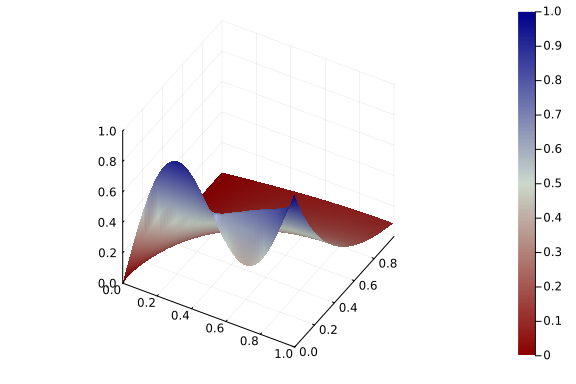
\includegraphics[width=\linewidth]{/figures/Chapter5_4_1.pdf}

\begin{lstlisting}
(*@\HLJLnd{@gif}@*) (*@\HLJLk{for}@*) (*@\HLJLn{i}@*) (*@\HLJLoB{=}@*) (*@\HLJLni{2}@*)(*@\HLJLoB{:}@*)(*@\HLJLni{50}@*)(*@\HLJLoB{:}@*)(*@\HLJLn{nt}@*)(*@\HLJLoB{+}@*)(*@\HLJLni{1}@*) 
    (*@\HLJLnf{plot}@*)(*@\HLJLp{(}@*)(*@\HLJLn{x}@*)(*@\HLJLp{,}@*) (*@\HLJLn{u}@*)(*@\HLJLp{[}@*)(*@\HLJLni{1}@*)(*@\HLJLp{,}@*)(*@\HLJLoB{:}@*)(*@\HLJLp{],}@*) (*@\HLJLn{size}@*) (*@\HLJLoB{=}@*) (*@\HLJLp{(}@*)(*@\HLJLni{500}@*)(*@\HLJLp{,}@*) (*@\HLJLni{150}@*)(*@\HLJLp{),}@*) (*@\HLJLn{label}@*) (*@\HLJLoB{=}@*) (*@\HLJLs{"{}u0"{}}@*)(*@\HLJLp{)}@*)
    (*@\HLJLnf{plot!}@*)(*@\HLJLp{(}@*)(*@\HLJLn{x}@*)(*@\HLJLp{,}@*) (*@\HLJLn{u}@*)(*@\HLJLp{[}@*)(*@\HLJLn{i}@*)(*@\HLJLp{,}@*)(*@\HLJLoB{:}@*)(*@\HLJLp{],}@*) (*@\HLJLn{label}@*) (*@\HLJLoB{=}@*) (*@\HLJLs{"{}t}@*) (*@\HLJLs{=}@*) (*@\HLJLs{"{}}@*) (*@\HLJLoB{*}@*) (*@\HLJLp{(}@*)(*@\HLJLnd{@sprintf}@*)(*@\HLJLp{(}@*)(*@\HLJLs{"{}{\%}.2f"{}}@*)(*@\HLJLp{,}@*) (*@\HLJLn{t}@*)(*@\HLJLp{[}@*)(*@\HLJLn{i}@*)(*@\HLJLp{])),}@*) (*@\HLJLn{legend}@*) (*@\HLJLoB{=}@*) (*@\HLJLsc{:outertopright}@*)(*@\HLJLp{)}@*)
(*@\HLJLk{end}@*)
\end{lstlisting}

\begin{lstlisting}
Plots.AnimatedGif((*@{"{}}@*)C:(*@{{\textbackslash}}@*)(*@{{\textbackslash}}@*)Users(*@{{\textbackslash}}@*)(*@{{\textbackslash}}@*)mfaso(*@{{\textbackslash}}@*)(*@{{\textbackslash}}@*)AppData(*@{{\textbackslash}}@*)(*@{{\textbackslash}}@*)Local(*@{{\textbackslash}}@*)(*@{{\textbackslash}}@*)Temp(*@{{\textbackslash}}@*)(*@{{\textbackslash}}@*)jl(*@{{\_}}@*)DFqKAnXEy2.gi
f(*@{"{}}@*))
\end{lstlisting}


\begin{lstlisting}
(*@\HLJLn{xx}@*) (*@\HLJLoB{=}@*) (*@\HLJLn{x}@*)(*@\HLJLoB{{\textquotesingle}}@*) (*@\HLJLoB{.*}@*) (*@\HLJLnf{ones}@*)(*@\HLJLp{(}@*)(*@\HLJLn{nt}@*)(*@\HLJLoB{+}@*)(*@\HLJLni{1}@*)(*@\HLJLp{)}@*)
(*@\HLJLn{tt}@*) (*@\HLJLoB{=}@*) (*@\HLJLnf{ones}@*)(*@\HLJLp{(}@*)(*@\HLJLn{nx}@*)(*@\HLJLoB{+}@*)(*@\HLJLni{2}@*)(*@\HLJLp{)}@*)(*@\HLJLoB{{\textquotesingle}}@*) (*@\HLJLoB{.*}@*) (*@\HLJLn{t}@*)
(*@\HLJLn{ue}@*) (*@\HLJLoB{=}@*) (*@\HLJLp{(}@*)(*@\HLJLn{x}@*)(*@\HLJLp{,}@*)(*@\HLJLn{t}@*)(*@\HLJLp{)}@*) (*@\HLJLoB{->}@*) (*@\HLJLnf{exp}@*)(*@\HLJLp{(}@*)(*@\HLJLoB{-}@*)(*@\HLJLn{\ensuremath{\pi}}@*)(*@\HLJLoB{{\textasciicircum}}@*)(*@\HLJLni{2}@*)(*@\HLJLoB{*}@*)(*@\HLJLn{t}@*)(*@\HLJLoB{/}@*)(*@\HLJLni{4}@*)(*@\HLJLp{)}@*)(*@\HLJLoB{*}@*)(*@\HLJLnf{sin}@*)(*@\HLJLp{(}@*)(*@\HLJLn{\ensuremath{\pi}}@*)(*@\HLJLoB{*}@*)(*@\HLJLn{x}@*)(*@\HLJLoB{/}@*)(*@\HLJLni{2}@*)(*@\HLJLp{)}@*) (*@\HLJLoB{+}@*) (*@\HLJLnfB{0.5}@*)(*@\HLJLoB{*}@*)(*@\HLJLnf{exp}@*)(*@\HLJLp{(}@*)(*@\HLJLoB{-}@*)(*@\HLJLni{4}@*)(*@\HLJLoB{*}@*)(*@\HLJLn{\ensuremath{\pi}}@*)(*@\HLJLoB{{\textasciicircum}}@*)(*@\HLJLni{2}@*)(*@\HLJLoB{*}@*)(*@\HLJLn{t}@*)(*@\HLJLp{)}@*)(*@\HLJLoB{*}@*)(*@\HLJLnf{sin}@*)(*@\HLJLp{(}@*)(*@\HLJLni{2}@*)(*@\HLJLn{\ensuremath{\pi}}@*)(*@\HLJLoB{*}@*)(*@\HLJLn{x}@*)(*@\HLJLp{)}@*)
(*@\HLJLn{error}@*) (*@\HLJLoB{=}@*) (*@\HLJLn{ue}@*)(*@\HLJLoB{.}@*)(*@\HLJLp{(}@*)(*@\HLJLn{xx}@*)(*@\HLJLp{,}@*)(*@\HLJLn{tt}@*)(*@\HLJLp{)}@*) (*@\HLJLoB{-}@*) (*@\HLJLn{u}@*) 
(*@\HLJLn{e1}@*) (*@\HLJLoB{=}@*) (*@\HLJLnf{maximum}@*)(*@\HLJLp{(}@*)(*@\HLJLn{error}@*)(*@\HLJLp{)}@*)
\end{lstlisting}

\begin{lstlisting}
0.00047001331601359553
\end{lstlisting}


If we double $n_x$, the the error decreases by roughly a factor of $4$.


\begin{lstlisting}
(*@\HLJLn{nx}@*) (*@\HLJLoB{*=}@*) (*@\HLJLni{2}@*)
(*@\HLJLn{u}@*)(*@\HLJLp{,}@*)(*@\HLJLn{x}@*)(*@\HLJLp{,}@*)(*@\HLJLn{t}@*) (*@\HLJLoB{=}@*) (*@\HLJLnf{Euler}@*)(*@\HLJLp{(}@*)(*@\HLJLn{f}@*)(*@\HLJLp{,}@*)(*@\HLJLn{\ensuremath{\phi}0}@*)(*@\HLJLp{,}@*)(*@\HLJLn{\ensuremath{\phi}1}@*)(*@\HLJLp{,}@*)(*@\HLJLn{nx}@*)(*@\HLJLp{,}@*)(*@\HLJLn{\ensuremath{\mu}}@*)(*@\HLJLp{,}@*)(*@\HLJLn{T}@*)(*@\HLJLp{)}@*)
(*@\HLJLnd{@show}@*) (*@\HLJLn{nt}@*) (*@\HLJLoB{=}@*) (*@\HLJLnf{length}@*)(*@\HLJLp{(}@*)(*@\HLJLn{t}@*)(*@\HLJLp{)}@*) (*@\HLJLoB{-}@*) (*@\HLJLni{1}@*)
(*@\HLJLn{xx}@*) (*@\HLJLoB{=}@*) (*@\HLJLn{x}@*)(*@\HLJLoB{{\textquotesingle}}@*) (*@\HLJLoB{.*}@*) (*@\HLJLnf{ones}@*)(*@\HLJLp{(}@*)(*@\HLJLn{nt}@*)(*@\HLJLoB{+}@*)(*@\HLJLni{1}@*)(*@\HLJLp{)}@*)
(*@\HLJLn{tt}@*) (*@\HLJLoB{=}@*) (*@\HLJLnf{ones}@*)(*@\HLJLp{(}@*)(*@\HLJLn{nx}@*)(*@\HLJLoB{+}@*)(*@\HLJLni{2}@*)(*@\HLJLp{)}@*)(*@\HLJLoB{{\textquotesingle}}@*) (*@\HLJLoB{.*}@*) (*@\HLJLn{t}@*)
(*@\HLJLn{error}@*) (*@\HLJLoB{=}@*) (*@\HLJLn{ue}@*)(*@\HLJLoB{.}@*)(*@\HLJLp{(}@*)(*@\HLJLn{xx}@*)(*@\HLJLp{,}@*)(*@\HLJLn{tt}@*)(*@\HLJLp{)}@*) (*@\HLJLoB{-}@*) (*@\HLJLn{u}@*)
(*@\HLJLn{e2}@*) (*@\HLJLoB{=}@*) (*@\HLJLnf{maximum}@*)(*@\HLJLp{(}@*)(*@\HLJLn{error}@*)(*@\HLJLp{)}@*)
(*@\HLJLn{e1}@*)(*@\HLJLoB{/}@*)(*@\HLJLn{e2}@*)
\end{lstlisting}

\begin{lstlisting}
nt = length(t) - 1 = 20402
3.929469183388294
\end{lstlisting}


This suggests the error decays as $\mathcal{O}(n_x^{-2})$, $n_x \to \infty$.


\begin{lstlisting}
(*@\HLJLn{nx}@*) (*@\HLJLoB{=}@*) (*@\HLJLni{30}@*)
(*@\HLJLn{\ensuremath{\mu}}@*) (*@\HLJLoB{=}@*) (*@\HLJLnfB{0.51}@*)
(*@\HLJLn{u}@*)(*@\HLJLp{,}@*)(*@\HLJLn{x}@*)(*@\HLJLp{,}@*)(*@\HLJLn{t}@*) (*@\HLJLoB{=}@*) (*@\HLJLnf{Euler}@*)(*@\HLJLp{(}@*)(*@\HLJLn{f}@*)(*@\HLJLp{,}@*)(*@\HLJLn{\ensuremath{\phi}0}@*)(*@\HLJLp{,}@*)(*@\HLJLn{\ensuremath{\phi}1}@*)(*@\HLJLp{,}@*)(*@\HLJLn{nx}@*)(*@\HLJLp{,}@*)(*@\HLJLn{\ensuremath{\mu}}@*)(*@\HLJLp{,}@*)(*@\HLJLn{T}@*)(*@\HLJLp{);}@*)
\end{lstlisting}


\begin{lstlisting}
(*@\HLJLnf{surface}@*)(*@\HLJLp{(}@*)(*@\HLJLn{x}@*)(*@\HLJLp{,}@*)(*@\HLJLn{t}@*)(*@\HLJLp{[}@*)(*@\HLJLni{1}@*)(*@\HLJLoB{:}@*)(*@\HLJLni{30}@*)(*@\HLJLoB{:}@*)(*@\HLJLk{end}@*)(*@\HLJLp{],}@*)(*@\HLJLn{u}@*)(*@\HLJLp{[}@*)(*@\HLJLni{1}@*)(*@\HLJLoB{:}@*)(*@\HLJLni{30}@*)(*@\HLJLoB{:}@*)(*@\HLJLk{end}@*)(*@\HLJLp{,}@*)(*@\HLJLoB{:}@*)(*@\HLJLp{],}@*)(*@\HLJLn{seriescolor}@*)(*@\HLJLoB{=:}@*)(*@\HLJLn{redsblues}@*)(*@\HLJLp{,}@*) (*@\HLJLn{camera}@*)(*@\HLJLoB{=}@*)(*@\HLJLp{(}@*)(*@\HLJLni{30}@*)(*@\HLJLp{,}@*)(*@\HLJLni{40}@*)(*@\HLJLp{))}@*)
\end{lstlisting}

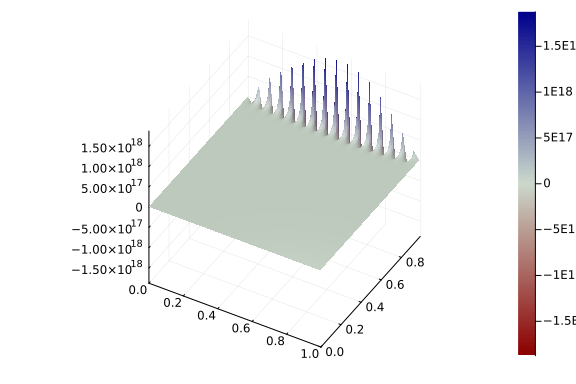
\includegraphics[width=\linewidth]{/figures/Chapter5_9_1.pdf}

\begin{lstlisting}
(*@\HLJLn{nt}@*) (*@\HLJLoB{=}@*) (*@\HLJLnf{length}@*)(*@\HLJLp{(}@*)(*@\HLJLn{t}@*)(*@\HLJLp{)}@*)(*@\HLJLoB{-}@*)(*@\HLJLni{1}@*)
(*@\HLJLnd{@gif}@*) (*@\HLJLk{for}@*) (*@\HLJLn{i}@*) (*@\HLJLoB{=}@*) (*@\HLJLni{2}@*)(*@\HLJLoB{:}@*)(*@\HLJLni{4}@*)(*@\HLJLoB{:}@*)(*@\HLJLn{nt}@*)(*@\HLJLoB{\ensuremath{\div}}@*)(*@\HLJLni{2}@*) 
    (*@\HLJLnf{plot}@*)(*@\HLJLp{(}@*)(*@\HLJLn{x}@*)(*@\HLJLp{,}@*) (*@\HLJLn{u}@*)(*@\HLJLp{[}@*)(*@\HLJLni{1}@*)(*@\HLJLp{,}@*)(*@\HLJLoB{:}@*)(*@\HLJLp{],}@*) (*@\HLJLn{size}@*) (*@\HLJLoB{=}@*) (*@\HLJLp{(}@*)(*@\HLJLni{500}@*)(*@\HLJLp{,}@*) (*@\HLJLni{150}@*)(*@\HLJLp{),}@*) (*@\HLJLn{label}@*) (*@\HLJLoB{=}@*) (*@\HLJLs{"{}u0"{}}@*)(*@\HLJLp{)}@*)
    (*@\HLJLnf{plot!}@*)(*@\HLJLp{(}@*)(*@\HLJLn{x}@*)(*@\HLJLp{,}@*) (*@\HLJLn{u}@*)(*@\HLJLp{[}@*)(*@\HLJLn{i}@*)(*@\HLJLp{,}@*)(*@\HLJLoB{:}@*)(*@\HLJLp{],}@*) (*@\HLJLn{label}@*) (*@\HLJLoB{=}@*) (*@\HLJLs{"{}t}@*) (*@\HLJLs{=}@*) (*@\HLJLs{"{}}@*) (*@\HLJLoB{*}@*) (*@\HLJLp{(}@*)(*@\HLJLnd{@sprintf}@*)(*@\HLJLp{(}@*)(*@\HLJLs{"{}{\%}.2f"{}}@*)(*@\HLJLp{,}@*) (*@\HLJLn{t}@*)(*@\HLJLp{[}@*)(*@\HLJLn{i}@*)(*@\HLJLp{])),}@*) (*@\HLJLn{legend}@*) (*@\HLJLoB{=}@*) (*@\HLJLsc{:outertopright}@*)(*@\HLJLp{)}@*)
(*@\HLJLk{end}@*)
\end{lstlisting}

\begin{lstlisting}
Plots.AnimatedGif((*@{"{}}@*)C:(*@{{\textbackslash}}@*)(*@{{\textbackslash}}@*)Users(*@{{\textbackslash}}@*)(*@{{\textbackslash}}@*)mfaso(*@{{\textbackslash}}@*)(*@{{\textbackslash}}@*)AppData(*@{{\textbackslash}}@*)(*@{{\textbackslash}}@*)Local(*@{{\textbackslash}}@*)(*@{{\textbackslash}}@*)Temp(*@{{\textbackslash}}@*)(*@{{\textbackslash}}@*)jl(*@{{\_}}@*)FD1jIvXmpz.gi
f(*@{"{}}@*))
\end{lstlisting}


\textbf{Note:} The gif animations don't appear in the PDF version of this chapter, however they can be viewed in the html version, which is available on Blackboard.

Based on these experiments, we conjecture that Euler's method converges if $\mu \leq \frac{1}{2}$.

The initial condition is "smoothed out" by the diffusion equation.  Here is another example:


\begin{lstlisting}
(*@\HLJLn{f}@*) (*@\HLJLoB{=}@*) (*@\HLJLn{x}@*) (*@\HLJLoB{->}@*) (*@\HLJLn{x}@*) (*@\HLJLoB{<=}@*) (*@\HLJLnfB{0.5}@*) (*@\HLJLoB{?}@*) (*@\HLJLni{2}@*)(*@\HLJLoB{*}@*)(*@\HLJLn{x}@*) (*@\HLJLoB{:}@*) (*@\HLJLni{2}@*)(*@\HLJLoB{-}@*)(*@\HLJLni{2}@*)(*@\HLJLoB{*}@*)(*@\HLJLn{x}@*)
(*@\HLJLn{\ensuremath{\phi}1}@*) (*@\HLJLoB{=}@*) (*@\HLJLn{t}@*) (*@\HLJLoB{->}@*) (*@\HLJLni{0}@*)
(*@\HLJLn{\ensuremath{\phi}0}@*) (*@\HLJLoB{=}@*) (*@\HLJLn{t}@*) (*@\HLJLoB{->}@*) (*@\HLJLni{0}@*)
(*@\HLJLn{nx}@*) (*@\HLJLoB{=}@*) (*@\HLJLni{19}@*)
(*@\HLJLn{\ensuremath{\mu}}@*) (*@\HLJLoB{=}@*) (*@\HLJLnfB{0.50}@*)
(*@\HLJLn{T}@*) (*@\HLJLoB{=}@*) (*@\HLJLnfB{0.25}@*)
(*@\HLJLn{u}@*)(*@\HLJLp{,}@*)(*@\HLJLn{x}@*)(*@\HLJLp{,}@*)(*@\HLJLn{t}@*) (*@\HLJLoB{=}@*) (*@\HLJLnf{Euler}@*)(*@\HLJLp{(}@*)(*@\HLJLn{f}@*)(*@\HLJLp{,}@*)(*@\HLJLn{\ensuremath{\phi}0}@*)(*@\HLJLp{,}@*)(*@\HLJLn{\ensuremath{\phi}1}@*)(*@\HLJLp{,}@*)(*@\HLJLn{nx}@*)(*@\HLJLp{,}@*)(*@\HLJLn{\ensuremath{\mu}}@*)(*@\HLJLp{,}@*)(*@\HLJLn{T}@*)(*@\HLJLp{);}@*)
\end{lstlisting}


\begin{lstlisting}
(*@\HLJLnf{surface}@*)(*@\HLJLp{(}@*)(*@\HLJLn{x}@*)(*@\HLJLp{,}@*)(*@\HLJLn{t}@*)(*@\HLJLp{[}@*)(*@\HLJLni{1}@*)(*@\HLJLoB{:}@*)(*@\HLJLni{30}@*)(*@\HLJLoB{:}@*)(*@\HLJLk{end}@*)(*@\HLJLp{],}@*)(*@\HLJLn{u}@*)(*@\HLJLp{[}@*)(*@\HLJLni{1}@*)(*@\HLJLoB{:}@*)(*@\HLJLni{30}@*)(*@\HLJLoB{:}@*)(*@\HLJLk{end}@*)(*@\HLJLp{,}@*)(*@\HLJLoB{:}@*)(*@\HLJLp{],}@*)(*@\HLJLn{seriescolor}@*)(*@\HLJLoB{=:}@*)(*@\HLJLn{redsblues}@*)(*@\HLJLp{,}@*) (*@\HLJLn{camera}@*)(*@\HLJLoB{=}@*)(*@\HLJLp{(}@*)(*@\HLJLni{30}@*)(*@\HLJLp{,}@*)(*@\HLJLni{40}@*)(*@\HLJLp{))}@*)
\end{lstlisting}

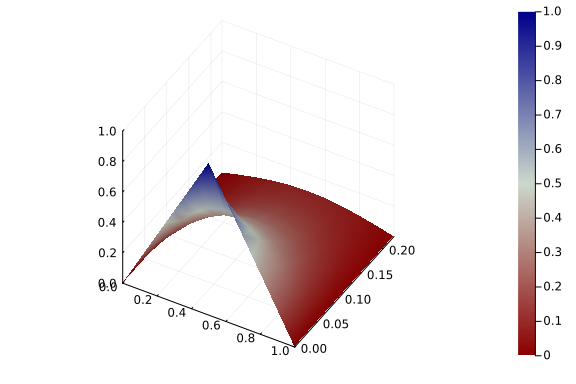
\includegraphics[width=\linewidth]{/figures/Chapter5_12_1.pdf}

\begin{lstlisting}
(*@\HLJLn{nt}@*) (*@\HLJLoB{=}@*) (*@\HLJLnf{length}@*)(*@\HLJLp{(}@*)(*@\HLJLn{t}@*)(*@\HLJLp{)}@*)(*@\HLJLoB{-}@*)(*@\HLJLni{1}@*)
(*@\HLJLnd{@gif}@*) (*@\HLJLk{for}@*) (*@\HLJLn{i}@*) (*@\HLJLoB{=}@*) (*@\HLJLni{2}@*)(*@\HLJLoB{:}@*)(*@\HLJLn{nt}@*) 
    (*@\HLJLnf{plot}@*)(*@\HLJLp{(}@*)(*@\HLJLn{x}@*)(*@\HLJLp{,}@*) (*@\HLJLn{u}@*)(*@\HLJLp{[}@*)(*@\HLJLni{1}@*)(*@\HLJLp{,}@*)(*@\HLJLoB{:}@*)(*@\HLJLp{],}@*) (*@\HLJLn{size}@*) (*@\HLJLoB{=}@*) (*@\HLJLp{(}@*)(*@\HLJLni{500}@*)(*@\HLJLp{,}@*) (*@\HLJLni{150}@*)(*@\HLJLp{),}@*) (*@\HLJLn{label}@*) (*@\HLJLoB{=}@*) (*@\HLJLs{"{}u0"{}}@*)(*@\HLJLp{)}@*)
    (*@\HLJLnf{plot!}@*)(*@\HLJLp{(}@*)(*@\HLJLn{x}@*)(*@\HLJLp{,}@*) (*@\HLJLn{u}@*)(*@\HLJLp{[}@*)(*@\HLJLn{i}@*)(*@\HLJLp{,}@*)(*@\HLJLoB{:}@*)(*@\HLJLp{],}@*) (*@\HLJLn{label}@*) (*@\HLJLoB{=}@*) (*@\HLJLs{"{}t}@*) (*@\HLJLs{=}@*) (*@\HLJLs{"{}}@*) (*@\HLJLoB{*}@*) (*@\HLJLp{(}@*)(*@\HLJLnd{@sprintf}@*)(*@\HLJLp{(}@*)(*@\HLJLs{"{}{\%}.2f"{}}@*)(*@\HLJLp{,}@*) (*@\HLJLn{t}@*)(*@\HLJLp{[}@*)(*@\HLJLn{i}@*)(*@\HLJLp{])),}@*) (*@\HLJLn{legend}@*) (*@\HLJLoB{=}@*) (*@\HLJLsc{:outertopright}@*)(*@\HLJLp{)}@*)
(*@\HLJLk{end}@*)
\end{lstlisting}

\begin{lstlisting}
Plots.AnimatedGif((*@{"{}}@*)C:(*@{{\textbackslash}}@*)(*@{{\textbackslash}}@*)Users(*@{{\textbackslash}}@*)(*@{{\textbackslash}}@*)mfaso(*@{{\textbackslash}}@*)(*@{{\textbackslash}}@*)AppData(*@{{\textbackslash}}@*)(*@{{\textbackslash}}@*)Local(*@{{\textbackslash}}@*)(*@{{\textbackslash}}@*)Temp(*@{{\textbackslash}}@*)(*@{{\textbackslash}}@*)jl(*@{{\_}}@*)jrl9HN0TW3.gi
f(*@{"{}}@*))
\end{lstlisting}


\subsubsection{Convergence of Euler's method}
\textbf{Proposition} If $\mu \leq \frac{1}{2}$, then Euler's method converges.

\textbf{Proof} Recall that

\[
\frac{\tilde{u}^{i+1}_j - \tilde{u}^i_j}{\tau} - \frac{\tilde{u}^{i}_{j+1} - 2\tilde{u}^i_j + \tilde{u}^i_{j-1}}{h^2}  =  \mathcal{O}(h^2), \qquad h \to 0,
\]
which implies

\[
\tilde{u}^{i+1}_j = \tilde{u}^i_j + \mu \left(\tilde{u}^{i}_{j+1} - 2\tilde{u}^i_j + \tilde{u}^i_{j-1}\right)  +  \mathcal{O}(h^4), \qquad h \to 0.
\]
Let $e^i_j = \tilde{u}^i_j - u^i_j$, then since

\[
u^{i+1}_j = u^i_j + \mu \left( u^{i}_{j+1} - 2u^i_j + u^i_{j-1}  \right),
\]
we have

\[
e^{i+1}_j = e^i_j + \mu \left( e^{i}_{j+1} - 2e^i_j + e^i_{j-1}  \right) + \mathcal{O}(h^4), \qquad h \to 0.
\]
This means that for sufficiently small $h > 0$, there exists a constant $c$ such that 

\[
\left\vert e^{i+1}_j -  e^i_j - \mu \left( e^{i}_{j+1} - 2e^i_j + e^i_{j-1}  \right) \right\vert  \leq ch^4.
\]
Hence, for sufficiently small $h$, we have


\begin{eqnarray*}
\vert e^{i+1}_j \vert &\leq& \left\vert e^i_j + \mu ( e^{i}_{j+1} - 2e^i_j + e^i_{j-1} ) \right\vert + ch^4\\
 & \leq & \mu \vert e^i_{j-1} \vert + \vert 1 - 2\mu \vert \vert e^i_{j} \vert  + \mu \vert e^i_{j+1} \vert + ch^4  \\
 & \leq & \left(2\mu  + \vert 1 - 2\mu \vert \right) \eta^i  + ch^4  
\end{eqnarray*}
where 

\[
\eta^{i} = \max_{j = 0, \ldots, n_x+1}\vert e^i_j \vert.
\]
The above inequality holds for $\vert e^{i+1}_j \vert$, with $j = 0, \ldots, n_x+1$ and therefore it also holds for $\vert  \eta^{i+1} \vert$. Since $0 < \mu \leq 1/2$ and $u^0_j = \tilde{u}^0_j$, which implies that $\eta^0=0$, we have that

\[
\eta^{i+1} \leq \eta^i  + ch^4 \leq \eta^{i-1} + 2ch^4 \leq \cdots \leq \eta^{0} + (i+1)ch^4 = (i+1)ch^4.
\]
Therefore

\[
\eta^{n_t} \leq c n_th^4 = \frac{c}{\mu} n_t\mu h^4 = \frac{c}{\mu} n_t\tau h^2 = \frac{c}{\mu}T h^2 
\]
We conclude that $\eta^i \to 0$ for $i = 0, \ldots, n_t$ as $h \to 0$ and therefore $e^i_j \to 0$ as $h \to 0$ for $j = 0, \ldots, n_x + 1$ and $i = 0, \ldots, n_t$ as $h \to 0$, which implies that the method converges.   $\blacksquare$

\textbf{Remark:} Notice that the maximum error of the Euler method (assuming all relevant partial derivatives exist and are bounded) is bounded by $\frac{c}{\mu}T h^2$ for sufficiently small $h$. This confirms our numerical observation above that the method converges at the rate $\mathcal{O}(h^2)$ as $h \to 0$, or equivalently, at the rate $\mathcal{O}(n_x^{-2})$ as $n_x \to \infty$ (i.e., the method is second order).

\subsubsection{Well-posedness and ill-posedness of PDE problems}
A PDE intial and / or boundary value problem is \textbf{well-posed} if there exists a unique solution that depends continuously on the initial and boundary data.  Otherwise, the PDE problem is said to be \textbf{ill-posed}.

\textbf{Example:}  Suppose $\varphi_0(t) = \varphi_1(t) = 0$ (i.e., zero Dirichlet boundary conditions), then using the method of separation of variables, it can be shown that if

\[
u(x,0) = f(x) = \sum_{m = 1}^{\infty}\alpha_m \sin \pi m x, \qquad 0 \leq x \leq 1,
\]
then the solution to the diffusion equation is

\[
u(x,t) = \sum_{m = 1}^{\infty}\alpha_m {\rm e}^{-\pi^2m^2 t} \sin \pi m x, \qquad 0 \leq x \leq 1, \qquad t \geq 0.
\]
The $2$-norm of a function $g$ on $[0, 1]$, or $L^2$ norm, is defined as

\[
\| g \|_2 = \left( \int_0^1 \left[g(x)\right]^2\,{\rm d}x   \right)^{1/2}
\]
Hence,


\begin{eqnarray*}
\|u(x,t)\|_2^2 &=& \int_0^1 \left[u(x,t)\right]^2\,{\rm d}x  = \int_0^1 \left(\sum_{m = 1}^{\infty}\alpha_m {\rm e}^{-\pi^2m^2 t} \sin \pi m x  \right)^2\,{\rm d}x \\
&=& \sum_{m=1}^{\infty}\sum_{j=1}^{\infty} \alpha_m \alpha_j{\rm e}^{-\pi^2(m^2 + j^2) t}\int_0^1 \sin\pi m x\sin \pi j x\, {\rm d}x
\end{eqnarray*}
and since

\[
\int_0^1 \sin \pi m x \sin \pi j x\, {\rm d}x = \begin{cases}
\frac{1}{2}, & m  = j, \\
0, & \text{otherwise}
\end{cases}
\]
we have

\[
\|u(x,t)\|_2^2 =  \frac{1}{2}\sum_{m=1}^{\infty} \alpha_m^2 {\rm e}^{-2\pi^2 m^2 t} \leq \frac{1}{2}\sum_{m=1}^{\infty} \alpha_m^2 = \| u(x,0) \|_2^2.
\]
Suppose that $\tilde{u}(x,t)$ is the solution to the diffusion equation with zero boundary conditions and a slightly perturbed initial condition, i.e.,

\[
\tilde{u}(x,0) = \tilde{f}(x) = \sum_{m = 1}^{\infty}\tilde{\alpha}_m \sin \pi m x, \qquad 0 \leq x \leq 1,
\]
where

\[
\| \tilde{u}(x,0) - u(x,0) \|_2^2 = \| \tilde{f}(x) - f(x) \|_2^2 = \frac{1}{2}\sum_{m=1}^{\infty} \left(  \tilde{\alpha}_m -    \alpha_m  \right)^2   \leq \epsilon^2 \ll 1
\]
then

\[
\tilde{u}(x,t) = \sum_{m = 1}^{\infty}\tilde{\alpha}_m {\rm e}^{-\pi^2m^2 t} \sin \pi m x, \qquad 0 \leq x \leq 1, \qquad t \geq 0
\]
and therefore

\[
\|\tilde{u}(x,t) - u(x,t)\|_2^2   \leq  \| \tilde{u}(x,0) -  u(x,0) \|_2^2 = \epsilon^2.
\]
This shows that if $\| \tilde{u}(x,0) -  u(x,0) \|_2$ is small, then $\|\tilde{u}(x,t) - u(x,t)\|_2$ is also small, which shows that the solution depends continuously on the initial data, i.e., the diffusion equation with zero Dirichlet boundary conditions is well-posed.

As an example of an ill-posed problem, consider the reversed-time diffusion equation:

\[
\frac{\partial u}{\partial t}=-\frac{\partial^2 u}{\partial x^2}, \qquad x \in (0, 1),\qquad t \in (0, T],
\]
subject to zero Dirichlet boundary conditions. If

\[
u(x,0) = f(x) = \sum_{m = 1}^{\infty}\alpha_m \sin \pi m x, \qquad 0 \leq x \leq 1,
\]
then

\[
u(x,t) = \sum_{m = 1}^{\infty}\alpha_m {\rm e}^{\pi^2m^2 t} \sin \pi m x, \qquad 0 \leq x \leq 1, \qquad t \geq 0.
\]
Now suppose we have initial data such that

\[
\alpha_m, \tilde{\alpha}_m = 0, \qquad m > N
\]
and

\[
\tilde{\alpha}_m -    \alpha_m  = \epsilon\sqrt{\frac{2}{N}}
\]
so that

\[
\| \tilde{u}(x,0) - u(x,0) \|_2^2 = \frac{1}{2}\sum_{m=1}^{N} \left(  \tilde{\alpha}_m -    \alpha_m  \right)^2     = \epsilon^2
\]
then for $t > 0$

\[
\|\tilde{u}(x,t) - u(x,t)\|_2^2 =  \frac{1}{2}\sum_{m=1}^{N} \left(\tilde{\alpha}_m - \alpha_m\right)^2 {\rm e}^{2\pi^2 m^2 t} = \frac{\epsilon^2}{N}\sum_{m=1}^{N} {\rm e}^{2\pi^2 m^2 t} \to \infty, \qquad N\to \infty.
\]
This shows that for an arbitrarily small perturbation of the initial data ($\|\tilde{u}(x,0) - u(x,0)\|_2 \leq \epsilon$) and for any $t > 0$, the difference between the solutions $u$ and $\tilde{u}$ at time $t$ can be made arbitrarily large by taking $N$ large enough. This shows that reversed-time diffusion equation is ill-posed because the solution does not depend continuously on the initial data.  In physics, the ill-posedness of the reversed-time diffusion equation is related to the impossibility of deducing the thermal history of an object from it present temperature distribution, which is studied in thermodynamics.

\subsubsection{Stability of numerical methods for PDEs}
A method is \textbf{stable} if, as $h \to 0$ and with $\mu$ constant,

\[
\vert u^i_j \vert < \infty, \qquad    j = 0, \ldots, n_x+1, \qquad i = 0, \ldots, n_t.
\]
The "Fundamental theorem of numerical analysis of differential equations" relates consistency, stability and convergence.

\textbf{Theorem (Lax equivalence theorem)} If a PDE problem is well posed, then a numerical method is convergent if and only if it is stable and consistent.

\paragraph{The von Neumann method for stability analysis}
The von Neumann method for the stability analysis of numerical methods for PDEs is applicable to linear PDEs and in its simplest form, it ignores boundary conditions. The method is essentially a discretised Fourier analysis.  The method proceeds as follows: given a numerical method for a PDE (e.g., a finite difference method), use the ansatz

\[
u^i_j = \lambda^i {\rm e}^{{\rm i}k x_j},
\]
where $k \in \mathbb{Z}$, $x_j = j h$, $j \in \mathbb{Z}$ and $h > 0$. 

\textbf{Note:} For the symbol $u^i_j$, $i$ is an index (a superscript), whereas $\lambda^i$ means $\lambda$ raised to the $i$-th power, where $i$ is a non-negative integer.  

Then for stability, we require

\[
\vert \lambda \vert \leq 1, \qquad  k \in \mathbb{Z}, \qquad h > 0
\]
because

\[
\vert u^i_j \vert = \vert \lambda^i {\rm e}^{{\rm i}k x_j} \vert = \vert \lambda^i \vert = \vert \lambda \vert^i.
\]
We only need to consider the one wave $u^i_j = \lambda^i {\rm e}^{{\rm i}k x_j}$ because we assume the PDE and thus also the discretised equations are linear and hence the principle of superposition holds. 

\textbf{Example} Here we illustrate the von Neumann method (or von Neumann stability analysis) for Euler's method:

\[
u^{i+1}_j = u^i_j + \mu \left( u^{i}_{j+1} - 2u^i_j + u^i_{j-1}  \right).
\]
Setting $u^i_j = \lambda^i {\rm e}^{{\rm i}k x_j}$, it follows that


\begin{eqnarray*}
\lambda &=& 1 + \mu\left({\rm e}^{{\rm i}kh} - 2 +  {\rm e}^{-{\rm i}kh}  \right)  \\
&=& 1 + \mu\left({\rm e}^{{\rm i}kh/2}  -  {\rm e}^{-{\rm i}kh/2}  \right)^2  \\
&=& 1 - 4\mu \sin^2(kh/2).
\end{eqnarray*}
For stability, we require

\[
\vert \lambda \vert \leq 1 \qquad \Leftrightarrow \qquad  -1 \leq  1 - 4\mu \sin^2(kh/2) \leq 1, \qquad h>0, \qquad k \in \mathbb{Z}.
\]
Since $0 \leq \sin^2(kh/2) \leq 1$ and $\mu > 0$, we conclude that Euler's method is stable if and only if $\mu \leq \frac{1}{2}$.

Earlier we proved from first principles that if $\mu \leq \frac{1}{2}$, then Euler's method converges. An alternative proof relies on the Lax equivalence theorem: first we show that Euler's method is consistent (which we've done already), then we show (using the von Neumann method) that the method is stable iff $\mu \leq \frac{1}{2}$ and then we can conclude that the method is convergent if $\mu \leq \frac{1}{2}$.

\paragraph{Stability analysis via matrix analysis}
We saw earlier that Euler's method can be formulated as

\[
\mathbf{u}^{i+1} = A\mathbf{u}^i + \mathbf{k}^i, \qquad i = 0, \ldots, n_t-1.
\]
where

\[
\mathbf{u}^i = \begin{bmatrix}
u^{i}_{1} \\
\vdots \\
u^{i}_{n_x}
\end{bmatrix}, \quad A = \begin{bmatrix}
1 - 2\mu & \mu & & & \\
\mu  & 1-2\mu & \mu  & & \\
      & \ddots & \ddots & \ddots & \\
      &        & \mu    & 1- 2\mu & \mu \\
      &        &        &\mu      & 1-2\mu
\end{bmatrix} \in \mathbb{R}^{n_x \times n_x}, \quad \mathbf{k}^i=
\begin{bmatrix}
\mu\varphi_0(t_i) \\
0 \\
\vdots \\
0 \\
\mu \varphi_1(t_i)
\end{bmatrix} \in \mathbb{R}^{n_x}.
\]
A large class of methods for the diffusion equation (and other linear PDEs) can be put into this form.  Before we analyse the stability of these methods using matrix methods, we recall some facts from linear algebra.

Recall the definition of the Euclidean inner product: let

\[
\mathbf{x} = \begin{bmatrix}
x_1 \\
\vdots \\
x_{n_x}
\end{bmatrix},  \mathbf{y} = \begin{bmatrix}
y_1 \\
\vdots \\
y_{n_x}
\end{bmatrix}  \in \mathbb{R}^{n_x}
\]
then

\[
\langle \mathbf{x}, \mathbf{y}\rangle = \mathbf{x}^{\top}\mathbf{y}
\]
If $\mathbf{x}, \mathbf{y} \in \mathbb{C}^{n_x}$, then

\[
\langle \mathbf{x}, \mathbf{y}\rangle = \overline{\mathbf{x}}^{\top}\mathbf{y} = \mathbf{x}^*\mathbf{y},
\]
i.e., $\mathbf{x}^*$ denotes the conjugate transpose of $\mathbf{x}$. This inner product induces the Euclidean or $\ell_2$ norm:

\[
\| \mathbf{x} \| = \left(\vert x_1\vert^2 + \cdots + \vert x_{n_x}\vert^2  \right)^{1/2}  = \left(\langle\mathbf{x},\mathbf{x}\rangle\right)^{1/2}.
\]
We shall also use a scaled Euclidean inner product and $\ell_2$ norm:

\[
\langle \mathbf{x}, \mathbf{y}\rangle_{h} := h\langle \mathbf{x}, \mathbf{y}\rangle
\]
and hence

\[
\| \mathbf{x} \|_h = \left(h\langle\mathbf{x},\mathbf{x}\rangle\right)^{1/2} = \sqrt{h}\,\| \mathbf{x}\|.
\]
where $h = \frac{1}{n_x+1}$ and $\mathbf{x}, \mathbf{y} \in \mathbb{C}^{n_x}$ or $\mathbf{x}, \mathbf{y} \in \mathbb{R}^{n_x}$.  One reason for using this inner product is the following: suppose the entries of $\mathbf{f} \in \mathbb{R}^{n_x}$ are the function values $f(x_j)$, $x_j = jh$, $j = 1, \ldots, n_x$, then from the Riemann sum definition of the integral of a function, it follows that as $h \to 0$

\[
\| \mathbf{f} \|_h = \left(h\sum_{j=1}^{n_x} [f(x_j)]^2  \right)^{1/2} \to \left( \int_0^1 [f(x)]^2 \,{\rm d}x  \right)^{1/2} = \| f\|_2.
\]
i.e., the scaled $\ell_2$ vector norm $\|\cdot \|_h$ tends to the $L^2$ function norm. There is another reason for using the scaled norm $\|\cdot \|_h$: suppose $\mathbf{x} \in \mathbb{R}^{n_x}$ is a vector such that each entry $x_j$ satisfies $x_j = \mathcal{O}(h^p)$, $h \to 0$, i.e., for sufficiently small $h$ (say $0 < h < h_0\ll 1$), there's a constant $c>0$ such that $\vert x_j \vert \leq c h^p$ for $j = 1, \ldots, n_x$, then for sufficiently small $h$,

\[
\| \mathbf{x} \|_h = \left(h\sum_{j=1}^{n_x} x_j^2  \right)^{1/2} \leq \left(hn_x c^2h^{2p}  \right)^{1/2} \leq ch^p
\]
i.e., $\| \mathbf{x} \|_h = \mathcal{O}(h^p)$, as $h \to 0$.

Let $A \in \mathbb{R}^{n_x \times n_x}$, then the matrix 2-norm or matrix Euclidean norm induced by the Euclidean or $\ell_2$ vector norm is

\[
\| A \| = \max_{\mathbf{x} \in \mathbb{R}^n, \mathbf{x}\neq \mathbf{0}} \frac{\| A\mathbf{x} \|}{\| \mathbf{x}\|} = \max_{\|\mathbf{x}\| =1} \| A\mathbf{x} \|.
\]
Since

\[
\frac{\| A\mathbf{x} \|}{\| \mathbf{x}\|} = \frac{\sqrt{h}\| A\mathbf{x} \|}{\sqrt{h}\| \mathbf{x}\|} =  \frac{\| A\mathbf{x} \|_h}{\| \mathbf{x}\|_h},
\]
if follows that 

\[
\| A \|_h = \| A \|.
\]
It follows from the definition of the matrix norm that

\[
\| A \mathbf{x}\| \leq \| A \| \| \mathbf{x} \|, \qquad \| A B\| \leq \| A\| \|B\|
\]
and the same is true in the norm $\| \cdot \|_h$.

The eigenvalues or \emph{spectrum} of a square matrix $A \in \mathbb{C}^{n_x \times n_x}$ is

\[
\sigma(A) = \left\lbrace \lambda \in \mathbb{C} : \det(A - \lambda I)= 0  \right\rbrace.
\]
The \emph{spectral radius} of a square matrix $A \in \mathbb{C}^{n_x \times n_x}$ is

\[
\rho(A) = \max\left\lbrace \vert \lambda \vert : \lambda \in \sigma(A)\right\rbrace
\]
A square matrix $A \in \mathbb{C}^{n_x \times n_x}$ is \textbf{normal} if $AA^{*} = A^{*}A$.  Recall that $A^*$ is the conjugate transpose of $A$, hence for  $A \in \mathbb{R}^{n_x \times n_x}$, $A^{*} = A^{\top}$ and thus a real matrix is normal if $AA^{\top} = A^{\top}A$.

If a matrix is normal, then

\[
\| A \|_h =\| A \| = \rho(A).
\]
A numerical method for the diffusion equation on $(x,t)\in [0, 1]\times[0, T]$ that takes the form

\[
\mathbf{u}^{i+1} = A\mathbf{u}^i + \mathbf{k}^i, \qquad i = 0, \ldots, n_t-1.
\]
where $\mathbf{u}^i \in \mathbb{R}^{n_x}$ and $A \in \mathbb{R}^{n_x \times n_x}$ is \textbf{stable} if there exists a $0 < c < \infty$ such that

\[
\lim_{h \to 0}\left( \max_{n = 0, 1, \ldots, n_t} \| A^n \|_h  \right) \leq c
\]
where, as before, $n_t\tau = T$, $h = 1/(n_x + 1)$, $\mu = \tau/h^2$ and $\mu$ is held constant.

\textbf{Theorem (stability for methods with normal matrices)} Suppose $A$ is normal, where $A \in \mathbb{R}^{n_x \times n_x}$ or $A \in \mathbb{C}^{n_x \times n_x}$,  then the method 

\[
\mathbf{u}^{i+1} = A\mathbf{u}^i + \mathbf{k}^i, \qquad i = 0, \ldots, n_t-1.
\]
is stable if there exists a $\nu \geq 0$ such that

\[
\rho(A) \leq {\rm e}^{\nu \tau}, \qquad h \to 0,
\]
where $\tau = \mu h^2$. 

\textbf{Proof}  For simplicity, let us assume that $A \in \mathbb{R}^{n_x \times n_x}$.  Using the definition of the scaled inner product $\langle \cdot, \cdot \rangle_h$, the normalcy of $A$ and the Cauchy-Schwarz inequality, it follows that for a $\mathbf{w} \in \mathbb{R}^{n_x}$, $\mathbf{w} \neq \mathbf{0}$,


\begin{eqnarray*}
\| A^n \mathbf{w} \|_h^2 &=& \langle A^n\mathbf{w}, A^n\mathbf{w}\rangle_h \\
&=& \langle \mathbf{w},  \left(A^n\right)^{\top}A^n\mathbf{w}\rangle_h \\
&=&  \langle \mathbf{w},  \left(A^{\top}A\right)^n\mathbf{w}\rangle_h \\ 
&\leq & \|  \mathbf{w}\|_h \|\left(A^{\top}A\right)^n\mathbf{w}\|_h \\
&\leq & \|  \mathbf{w}\|_h^2 \|\left(A^{\top}A\right)^n\|_h \\
&\leq & \|  \mathbf{w}\|_h^2 \|A\|_h^{2n}.
\end{eqnarray*}
Therefore, since $A$ is normal and $0 \leq  n \leq n_t$,

\[
\frac{\| A^n \mathbf{w} \|_h}{\|  \mathbf{w}\|_h} \leq \|A\|_h^{n} = \left[\rho(A)\right]^n \leq {\rm e}^{\nu n\tau}\leq  {\rm e}^{\nu n_t\tau} = {\rm e}^{\nu T}.
\]
Since 

\[
\|A^n \|_h = \max_{\mathbf{w}\in \mathbb{R}^{n_x}, \mathbf{w}\neq 0}\frac{\| A^n \mathbf{w} \|_h}{\|  \mathbf{w}\|_h},
\]
the result follows since we've shown that $\|A^n \|_h \leq c$ for $n = 0, \ldots, n_t$ with $c = {\rm e}^{\nu T}$ as $h \to 0$.  $\blacksquare$

\textbf{Example (Stability of Euler's method via matrix analysis)} For Euler's method, 

\[
 A = \begin{bmatrix}
1 - 2\mu & \mu & & & \\
\mu  & 1-2\mu & \mu  & & \\
      & \ddots & \ddots & \ddots & \\
      &        & \mu    & 1- 2\mu & \mu \\
      &        &        &\mu      & 1-2\mu
\end{bmatrix} \in \mathbb{R}^{n_x \times n_x}.
\]
Since $A$ is symmetric, it is a normal matrix.  However, $A$ is not just symmetric, it is a TST matrix (tridiagonal, symmetric and Toeplitz) and the eigenvalues of TST matrices are known explicitly: 

\textbf{Lemma (eigenvalues of TST matrices)} The eigenvalues of an $n_x \times n_x$ TST matrix with $\alpha$ on the main diagonal and $\beta$ on the first super- and sub-diagonal are

\[
\lambda_j = \alpha + 2\beta\cos\left( \frac{\pi j}{n_x+1}  \right), \qquad j = 1, \ldots, n_x.
\]
\textbf{Proof} See \emph{A First Course in the Numerical Analysis of Differential Equations} by A. Iserles, 2nd Edition, p. 264.

Returning to Euler's method, since $h = 1/(n_x+1)$ and $x_j = jh$, the eigenvalues of the matrix $A$ are

\[
\lambda_j = 1-2\mu + 2\mu\cos(\pi x_j) = 1-2\mu +2\mu(1 - 2\sin^2(\pi x_j/2)) = 1 - 4\mu\sin^2(\pi x_j/2) 
\]
for $j = 1, \ldots, n_x$.  If $0 < \mu \leq 1/2$, then $\rho(A) \leq 1$ as $h \to 0$ and hence the above theorem holds with $\nu = 0$ and we conclude that Euler's method is stable, whereas if $\mu > 1/2$, then $\rho(A) > 1$ as $h \to 0$ and there isn't a $\nu > 0$ such that the above theorem holds.


\begin{lstlisting}
(*@\HLJLn{nx}@*) (*@\HLJLoB{=}@*) (*@\HLJLni{11}@*)
(*@\HLJLn{\ensuremath{\mu}}@*) (*@\HLJLoB{=}@*) (*@\HLJLnfB{0.5}@*)
(*@\HLJLn{A}@*) (*@\HLJLoB{=}@*) (*@\HLJLnf{SymTridiagonal}@*)(*@\HLJLp{(}@*)(*@\HLJLnf{fill}@*)(*@\HLJLp{((}@*)(*@\HLJLni{1}@*) (*@\HLJLoB{-}@*) (*@\HLJLni{2}@*)(*@\HLJLn{\ensuremath{\mu}}@*)(*@\HLJLp{),}@*)(*@\HLJLn{nx}@*)(*@\HLJLp{),}@*)(*@\HLJLnf{fill}@*)(*@\HLJLp{(}@*)(*@\HLJLn{\ensuremath{\mu}}@*)(*@\HLJLp{,}@*)(*@\HLJLn{nx}@*)(*@\HLJLoB{-}@*)(*@\HLJLni{1}@*)(*@\HLJLp{))}@*)
(*@\HLJLn{h}@*) (*@\HLJLoB{=}@*) (*@\HLJLni{1}@*)(*@\HLJLoB{/}@*)(*@\HLJLp{(}@*)(*@\HLJLn{nx}@*)(*@\HLJLoB{+}@*)(*@\HLJLni{1}@*)(*@\HLJLp{)}@*)
(*@\HLJLn{x}@*) (*@\HLJLoB{=}@*) (*@\HLJLn{h}@*)(*@\HLJLoB{:}@*)(*@\HLJLn{h}@*)(*@\HLJLoB{:}@*)(*@\HLJLni{1}@*)(*@\HLJLoB{-}@*)(*@\HLJLn{h}@*)
(*@\HLJLp{[}@*)(*@\HLJLnf{eigvals}@*)(*@\HLJLp{(}@*)(*@\HLJLn{A}@*)(*@\HLJLp{)}@*) (*@\HLJLni{1}@*) (*@\HLJLoB{.-}@*) (*@\HLJLni{4}@*)(*@\HLJLn{\ensuremath{\mu}}@*)(*@\HLJLoB{*}@*)(*@\HLJLn{sin}@*)(*@\HLJLoB{.}@*)(*@\HLJLp{(}@*)(*@\HLJLn{\ensuremath{\pi}}@*)(*@\HLJLoB{*}@*)(*@\HLJLn{x}@*)(*@\HLJLp{[}@*)(*@\HLJLk{end}@*)(*@\HLJLoB{:-}@*)(*@\HLJLni{1}@*)(*@\HLJLoB{:}@*)(*@\HLJLni{1}@*)(*@\HLJLp{]}@*)(*@\HLJLoB{/}@*)(*@\HLJLni{2}@*)(*@\HLJLp{)}@*)(*@\HLJLoB{.{\textasciicircum}}@*)(*@\HLJLni{2}@*)(*@\HLJLp{]}@*)
\end{lstlisting}

\begin{lstlisting}
11(*@\ensuremath{\times}@*)2 Matrix(*@{{\{}}@*)Float64(*@{{\}}}@*):
 -0.965926     -0.965926
 -0.866025     -0.866025
 -0.707107     -0.707107
 -0.5          -0.5
 -0.258819     -0.258819
 -2.68965e-16   2.22045e-16
  0.258819      0.258819
  0.5           0.5
  0.707107      0.707107
  0.866025      0.866025
  0.965926      0.965926
\end{lstlisting}


\subsection{Implicit Euler method}
Recall that we arrived at Euler's method for the diffusion equation by combining a (first-order) forward difference approximation to the time derivative with a (second-order) central difference approximation to the second spatial derivative.  Suppose now that we approximate the time derivative with a (first-order) \emph{backward} difference approximation 

\[
u_t(x_j,t_i) \approx \frac{u^{i}_j - u^{i-1}_j}{\tau}
\]
and again use a second-order central difference approximation to $u_{xx}$, then we arrive at the method

\[
\frac{u^{i}_j - u^{i-1}_j}{\tau} - \frac{u^{i}_{j+1} - 2u^i_j + u^i_{j-1}}{h^2} = 0
\]
or

\[
u^{i}_j = u^{i+1}_j - \mu \left( u^{i+1}_{j+1} - 2u^{i+1}_j + u^{i+1}_{j-1}  \right), \qquad j = 1, \ldots, n_x,
\]
which is known is the backward Euler method, or the implicit Euler method.

In linear algebra notation, the method becomes

\[
B\mathbf{u}^{i+1} = \mathbf{u}^i + \mathbf{k}^{i+1}
\]
where

\[
\mathbf{u}^i = \begin{bmatrix}
u^{i}_{1} \\
\vdots \\
u^{i}_{n_x}
\end{bmatrix}, \quad  B = \begin{bmatrix}
1 + 2\mu & -\mu & & & \\
-\mu  & 1+2\mu & -\mu  & & \\
      & \ddots & \ddots & \ddots & \\
      &        & -\mu    & 1+ 2\mu & -\mu \\
      &        &        &-\mu      & 1+2\mu
\end{bmatrix} \in \mathbb{R}^{n_x \times n_x}, \quad \mathbf{k}^i=
\begin{bmatrix}
\mu\varphi_0(t_i) \\
0 \\
\vdots \\
0 \\
\mu \varphi_1(t_i)
\end{bmatrix} \in \mathbb{R}^{n_x}.
\]
As with the (explicit) Euler method, the local truncation error is second order

\[
\frac{\tilde{u}^{i}_j - \tilde{u}^{i-1}_j}{\tau} - \frac{\tilde{u}^{i}_{j+1} - 2\tilde{u}^i_j + \tilde{u}^i_{j-1}}{h^2} =  \mathcal{O}(h^2), \qquad h \to 0,
\]
and therefore the method is consistent.  There appears to be no reason to prefer the implicit Euler method over the explicit Euler method because it has the same order but it is computationally more expensive.   Now, let's consider the stability of the implicit Euler method. 

\subsubsection{Von Neumann stability analysis}
Setting

\[
u^i_j = \lambda^i{\rm e}^{{\rm i}k x_j}
\]
in the implicit Euler method, we deduce that


\begin{eqnarray*}
1 &=& \lambda\left[1 - \mu\left({\rm e}^{{\rm i}kh} - 2 + {\rm e}^{-{\rm i}kh} \right)\right] \\
&=& \lambda\left[1 - \mu\left({\rm e}^{{\rm i}kh/2} - {\rm e}^{-{\rm i}kh/2} \right)^2\right] \\
&=& \lambda\left[1 + 4\mu\sin^2(kh/2)\right].
\end{eqnarray*}
For stability, we require

\[
\vert \lambda \vert \leq 1 \qquad \Leftrightarrow \qquad 1 + 4\mu\sin^2(kh/2) \geq 1, \qquad h>0, \qquad k \in \mathbb{Z}.
\]
We conclude that the backward Euler method is stable for all $\mu > 0$.  We say that the backward Euler method is unconditionally stable.  Hence, compared to the explicit Euler method, we can take much larger step sizes while maintaining stability.   However, larger step sizes lead to larger errors.   The ideal method would be high order and unconditionally stable.

\subsubsection{Stability analysis via matrix analysis}
The implicit Euler method can be formulated as

\[
\mathbf{u}^{i+1} = A\mathbf{u}^i + \mathbf{b}^i
\]
where $A = B^{-1}$ and $\mathbf{b}^i = B^{-1}\mathbf{k}^{i+1}$.  

The matrix $A$ is normal because

\[
AA^{\top} = B^{-1}B^{-\top} = \left(B^{\top}B  \right)^{-1} = \left(B B^T  \right)^{-1} = B^{-\top}B^{-1} = A^{\top}A.
\]
Since $B$ is a TST matrix, its eigenvalues are

\[
\lambda_j = 1 + 2\mu - 2\mu\cos\left(\pi x_j  \right) = 1 + 2\mu -2\mu(1 - 2\sin^2(\pi x_j/2)) = 1 + 4\mu\sin^2(\pi x_j/2).
\]
Since $\lambda \in \sigma(B)$ iff $\lambda^{-1} \in \sigma(B^{-1})$, we conclude that for any $\mu > 0$ and $h > 0$ 

\[
\rho(A) = \max_{j = 1, \ldots, n_x} \frac{1}{1 + 4\mu \sin^2(\pi x_j/2)} < 1, 
\]
and therefore the implicit Euler method is stable for any $\mu > 0$.


\begin{lstlisting}
(*@\HLJLn{nx}@*) (*@\HLJLoB{=}@*) (*@\HLJLni{11}@*)
(*@\HLJLn{\ensuremath{\mu}}@*) (*@\HLJLoB{=}@*) (*@\HLJLnfB{0.5}@*)
(*@\HLJLn{B}@*) (*@\HLJLoB{=}@*) (*@\HLJLnf{SymTridiagonal}@*)(*@\HLJLp{(}@*)(*@\HLJLnf{fill}@*)(*@\HLJLp{((}@*)(*@\HLJLni{1}@*) (*@\HLJLoB{+}@*) (*@\HLJLni{2}@*)(*@\HLJLn{\ensuremath{\mu}}@*)(*@\HLJLp{),}@*)(*@\HLJLn{nx}@*)(*@\HLJLp{),}@*)(*@\HLJLnf{fill}@*)(*@\HLJLp{(}@*)(*@\HLJLoB{-}@*)(*@\HLJLn{\ensuremath{\mu}}@*)(*@\HLJLp{,}@*)(*@\HLJLn{nx}@*)(*@\HLJLoB{-}@*)(*@\HLJLni{1}@*)(*@\HLJLp{))}@*)
(*@\HLJLn{h}@*) (*@\HLJLoB{=}@*) (*@\HLJLni{1}@*)(*@\HLJLoB{/}@*)(*@\HLJLp{(}@*)(*@\HLJLn{nx}@*)(*@\HLJLoB{+}@*)(*@\HLJLni{1}@*)(*@\HLJLp{)}@*)
(*@\HLJLn{x}@*) (*@\HLJLoB{=}@*) (*@\HLJLn{h}@*)(*@\HLJLoB{:}@*)(*@\HLJLn{h}@*)(*@\HLJLoB{:}@*)(*@\HLJLni{1}@*)(*@\HLJLoB{-}@*)(*@\HLJLn{h}@*)
(*@\HLJLnf{norm}@*)(*@\HLJLp{(}@*)(*@\HLJLnf{eigvals}@*)(*@\HLJLp{(}@*)(*@\HLJLn{B}@*)(*@\HLJLp{)}@*) (*@\HLJLoB{-}@*) (*@\HLJLp{(}@*)(*@\HLJLni{1}@*) (*@\HLJLoB{.+}@*) (*@\HLJLni{4}@*)(*@\HLJLn{\ensuremath{\mu}}@*)(*@\HLJLoB{*}@*)(*@\HLJLn{sin}@*)(*@\HLJLoB{.}@*)(*@\HLJLp{(}@*)(*@\HLJLn{\ensuremath{\pi}}@*)(*@\HLJLoB{*}@*)(*@\HLJLn{x}@*)(*@\HLJLoB{/}@*)(*@\HLJLni{2}@*)(*@\HLJLp{)}@*)(*@\HLJLoB{.{\textasciicircum}}@*)(*@\HLJLni{2}@*)(*@\HLJLp{),}@*)(*@\HLJLn{Inf}@*)(*@\HLJLp{)}@*)
\end{lstlisting}

\begin{lstlisting}
1.3322676295501878e-15
\end{lstlisting}


\subsubsection{Numerical experiment}

\begin{lstlisting}
(*@\HLJLk{function}@*) (*@\HLJLnf{BackwardEuler}@*)(*@\HLJLp{(}@*)(*@\HLJLn{f}@*)(*@\HLJLp{,}@*)(*@\HLJLn{\ensuremath{\phi}0}@*)(*@\HLJLp{,}@*)(*@\HLJLn{\ensuremath{\phi}1}@*)(*@\HLJLp{,}@*)(*@\HLJLn{nx}@*)(*@\HLJLp{,}@*)(*@\HLJLn{\ensuremath{\mu}}@*)(*@\HLJLp{,}@*)(*@\HLJLn{T}@*)(*@\HLJLp{)}@*)
    
    (*@\HLJLn{x}@*) (*@\HLJLoB{=}@*) (*@\HLJLnf{range}@*)(*@\HLJLp{(}@*)(*@\HLJLni{0}@*)(*@\HLJLp{,}@*)(*@\HLJLni{1}@*)(*@\HLJLp{,}@*)(*@\HLJLn{nx}@*) (*@\HLJLoB{+}@*) (*@\HLJLni{2}@*)(*@\HLJLp{)}@*)
    (*@\HLJLn{h}@*) (*@\HLJLoB{=}@*) (*@\HLJLni{1}@*)(*@\HLJLoB{/}@*)(*@\HLJLp{(}@*)(*@\HLJLn{nx}@*)(*@\HLJLoB{+}@*)(*@\HLJLni{1}@*)(*@\HLJLp{)}@*)
    (*@\HLJLn{\ensuremath{\tau}}@*) (*@\HLJLoB{=}@*) (*@\HLJLn{\ensuremath{\mu}}@*)(*@\HLJLoB{*}@*)(*@\HLJLn{h}@*)(*@\HLJLoB{{\textasciicircum}}@*)(*@\HLJLni{2}@*)
    (*@\HLJLn{t}@*) (*@\HLJLoB{=}@*) (*@\HLJLni{0}@*)(*@\HLJLoB{:}@*)(*@\HLJLn{\ensuremath{\tau}}@*)(*@\HLJLoB{:}@*)(*@\HLJLn{T}@*)
    (*@\HLJLn{nt}@*) (*@\HLJLoB{=}@*) (*@\HLJLnf{length}@*)(*@\HLJLp{(}@*)(*@\HLJLn{t}@*)(*@\HLJLp{)}@*)(*@\HLJLoB{-}@*)(*@\HLJLni{1}@*)
    (*@\HLJLn{B}@*) (*@\HLJLoB{=}@*) (*@\HLJLnf{SymTridiagonal}@*)(*@\HLJLp{(}@*)(*@\HLJLnf{fill}@*)(*@\HLJLp{((}@*)(*@\HLJLni{1}@*) (*@\HLJLoB{+}@*) (*@\HLJLni{2}@*)(*@\HLJLn{\ensuremath{\mu}}@*)(*@\HLJLp{),}@*)(*@\HLJLn{nx}@*)(*@\HLJLp{),}@*)(*@\HLJLnf{fill}@*)(*@\HLJLp{(}@*)(*@\HLJLoB{-}@*)(*@\HLJLn{\ensuremath{\mu}}@*)(*@\HLJLp{,}@*)(*@\HLJLn{nx}@*)(*@\HLJLoB{-}@*)(*@\HLJLni{1}@*)(*@\HLJLp{))}@*)
    (*@\HLJLn{u}@*) (*@\HLJLoB{=}@*) (*@\HLJLnf{zeros}@*)(*@\HLJLp{(}@*)(*@\HLJLn{nt}@*)(*@\HLJLoB{+}@*)(*@\HLJLni{1}@*)(*@\HLJLp{,}@*)(*@\HLJLn{nx}@*)(*@\HLJLoB{+}@*)(*@\HLJLni{2}@*)(*@\HLJLp{)}@*)
    (*@\HLJLn{u}@*)(*@\HLJLp{[}@*)(*@\HLJLoB{:}@*)(*@\HLJLp{,}@*)(*@\HLJLni{1}@*)(*@\HLJLp{]}@*) (*@\HLJLoB{=}@*) (*@\HLJLn{\ensuremath{\phi}0}@*)(*@\HLJLoB{.}@*)(*@\HLJLp{(}@*)(*@\HLJLn{t}@*)(*@\HLJLp{)}@*)
    (*@\HLJLn{u}@*)(*@\HLJLp{[}@*)(*@\HLJLoB{:}@*)(*@\HLJLp{,}@*)(*@\HLJLn{nx}@*)(*@\HLJLoB{+}@*)(*@\HLJLni{2}@*)(*@\HLJLp{]}@*) (*@\HLJLoB{=}@*) (*@\HLJLn{\ensuremath{\phi}1}@*)(*@\HLJLoB{.}@*)(*@\HLJLp{(}@*)(*@\HLJLn{t}@*)(*@\HLJLp{)}@*)
    (*@\HLJLn{u}@*)(*@\HLJLp{[}@*)(*@\HLJLni{1}@*)(*@\HLJLp{,}@*)(*@\HLJLni{2}@*)(*@\HLJLoB{:}@*)(*@\HLJLn{nx}@*)(*@\HLJLoB{+}@*)(*@\HLJLni{1}@*)(*@\HLJLp{]}@*) (*@\HLJLoB{=}@*) (*@\HLJLn{f}@*)(*@\HLJLoB{.}@*)(*@\HLJLp{(}@*)(*@\HLJLn{x}@*)(*@\HLJLp{[}@*)(*@\HLJLni{2}@*)(*@\HLJLoB{:}@*)(*@\HLJLn{nx}@*)(*@\HLJLoB{+}@*)(*@\HLJLni{1}@*)(*@\HLJLp{])}@*)

    (*@\HLJLk{for}@*) (*@\HLJLn{i}@*) (*@\HLJLoB{=}@*) (*@\HLJLni{1}@*)(*@\HLJLoB{:}@*)(*@\HLJLn{nt}@*)
        (*@\HLJLn{b}@*) (*@\HLJLoB{=}@*) (*@\HLJLn{u}@*)(*@\HLJLp{[}@*)(*@\HLJLn{i}@*)(*@\HLJLp{,}@*)(*@\HLJLni{2}@*)(*@\HLJLoB{:}@*)(*@\HLJLn{nx}@*)(*@\HLJLoB{+}@*)(*@\HLJLni{1}@*)(*@\HLJLp{]}@*) 
        (*@\HLJLn{b}@*)(*@\HLJLp{[}@*)(*@\HLJLni{1}@*)(*@\HLJLp{]}@*) (*@\HLJLoB{+=}@*) (*@\HLJLn{\ensuremath{\mu}}@*)(*@\HLJLoB{*}@*)(*@\HLJLnf{\ensuremath{\phi}0}@*)(*@\HLJLp{(}@*)(*@\HLJLn{t}@*)(*@\HLJLp{[}@*)(*@\HLJLn{i}@*)(*@\HLJLoB{+}@*)(*@\HLJLni{1}@*)(*@\HLJLp{])}@*)
        (*@\HLJLn{b}@*)(*@\HLJLp{[}@*)(*@\HLJLn{nx}@*)(*@\HLJLp{]}@*) (*@\HLJLoB{+=}@*) (*@\HLJLn{\ensuremath{\mu}}@*)(*@\HLJLoB{*}@*)(*@\HLJLnf{\ensuremath{\phi}1}@*)(*@\HLJLp{(}@*)(*@\HLJLn{t}@*)(*@\HLJLp{[}@*)(*@\HLJLn{i}@*)(*@\HLJLoB{+}@*)(*@\HLJLni{1}@*)(*@\HLJLp{])}@*)
        (*@\HLJLn{u}@*)(*@\HLJLp{[}@*)(*@\HLJLn{i}@*)(*@\HLJLoB{+}@*)(*@\HLJLni{1}@*)(*@\HLJLp{,}@*)(*@\HLJLni{2}@*)(*@\HLJLoB{:}@*)(*@\HLJLn{nx}@*)(*@\HLJLoB{+}@*)(*@\HLJLni{1}@*)(*@\HLJLp{]}@*) (*@\HLJLoB{=}@*) (*@\HLJLn{B}@*)(*@\HLJLoB{{\textbackslash}}@*)(*@\HLJLn{b}@*)
    (*@\HLJLk{end}@*)
    
    (*@\HLJLn{u}@*)(*@\HLJLp{,}@*) (*@\HLJLn{x}@*)(*@\HLJLp{,}@*) (*@\HLJLn{t}@*)
(*@\HLJLk{end}@*)
\end{lstlisting}

\begin{lstlisting}
BackwardEuler (generic function with 1 method)
\end{lstlisting}


\begin{lstlisting}
(*@\HLJLn{f}@*) (*@\HLJLoB{=}@*) (*@\HLJLn{x}@*) (*@\HLJLoB{->}@*) (*@\HLJLnf{sin}@*)(*@\HLJLp{(}@*)(*@\HLJLn{\ensuremath{\pi}}@*)(*@\HLJLoB{*}@*)(*@\HLJLn{x}@*)(*@\HLJLoB{/}@*)(*@\HLJLni{2}@*)(*@\HLJLp{)}@*) (*@\HLJLoB{+}@*) (*@\HLJLnfB{0.5}@*)(*@\HLJLoB{*}@*)(*@\HLJLnf{sin}@*)(*@\HLJLp{(}@*)(*@\HLJLni{2}@*)(*@\HLJLn{\ensuremath{\pi}}@*)(*@\HLJLoB{*}@*)(*@\HLJLn{x}@*)(*@\HLJLp{)}@*)
(*@\HLJLn{\ensuremath{\phi}1}@*) (*@\HLJLoB{=}@*) (*@\HLJLn{t}@*) (*@\HLJLoB{->}@*) (*@\HLJLnf{exp}@*)(*@\HLJLp{(}@*)(*@\HLJLoB{-}@*)(*@\HLJLn{\ensuremath{\pi}}@*)(*@\HLJLoB{{\textasciicircum}}@*)(*@\HLJLni{2}@*)(*@\HLJLoB{*}@*)(*@\HLJLn{t}@*)(*@\HLJLoB{/}@*)(*@\HLJLni{4}@*)(*@\HLJLp{)}@*)
(*@\HLJLn{\ensuremath{\phi}0}@*) (*@\HLJLoB{=}@*) (*@\HLJLn{t}@*) (*@\HLJLoB{->}@*) (*@\HLJLni{0}@*)
(*@\HLJLn{nx}@*) (*@\HLJLoB{=}@*) (*@\HLJLni{50}@*)
(*@\HLJLn{\ensuremath{\mu}}@*) (*@\HLJLoB{=}@*) (*@\HLJLnfB{0.50}@*)
(*@\HLJLn{T}@*) (*@\HLJLoB{=}@*) (*@\HLJLni{1}@*)
(*@\HLJLnf{Euler}@*)(*@\HLJLp{(}@*)(*@\HLJLn{f}@*)(*@\HLJLp{,}@*)(*@\HLJLn{\ensuremath{\phi}0}@*)(*@\HLJLp{,}@*)(*@\HLJLn{\ensuremath{\phi}1}@*)(*@\HLJLp{,}@*)(*@\HLJLn{nx}@*)(*@\HLJLp{,}@*)(*@\HLJLn{\ensuremath{\mu}}@*)(*@\HLJLp{,}@*)(*@\HLJLn{T}@*)(*@\HLJLp{)}@*)
(*@\HLJLnd{@time}@*) (*@\HLJLnf{Euler}@*)(*@\HLJLp{(}@*)(*@\HLJLn{f}@*)(*@\HLJLp{,}@*)(*@\HLJLn{\ensuremath{\phi}0}@*)(*@\HLJLp{,}@*)(*@\HLJLn{\ensuremath{\phi}1}@*)(*@\HLJLp{,}@*)(*@\HLJLn{nx}@*)(*@\HLJLp{,}@*)(*@\HLJLn{\ensuremath{\mu}}@*)(*@\HLJLp{,}@*)(*@\HLJLn{T}@*)(*@\HLJLp{)}@*)
(*@\HLJLnf{BackwardEuler}@*)(*@\HLJLp{(}@*)(*@\HLJLn{f}@*)(*@\HLJLp{,}@*)(*@\HLJLn{\ensuremath{\phi}0}@*)(*@\HLJLp{,}@*)(*@\HLJLn{\ensuremath{\phi}1}@*)(*@\HLJLp{,}@*)(*@\HLJLn{nx}@*)(*@\HLJLp{,}@*)(*@\HLJLn{\ensuremath{\mu}}@*)(*@\HLJLp{,}@*)(*@\HLJLn{T}@*)(*@\HLJLp{)}@*)
(*@\HLJLn{u}@*)(*@\HLJLp{,}@*)(*@\HLJLn{x}@*)(*@\HLJLp{,}@*)(*@\HLJLn{t}@*) (*@\HLJLoB{=}@*) (*@\HLJLnd{@time}@*) (*@\HLJLnf{BackwardEuler}@*)(*@\HLJLp{(}@*)(*@\HLJLn{f}@*)(*@\HLJLp{,}@*)(*@\HLJLn{\ensuremath{\phi}0}@*)(*@\HLJLp{,}@*)(*@\HLJLn{\ensuremath{\phi}1}@*)(*@\HLJLp{,}@*)(*@\HLJLn{nx}@*)(*@\HLJLp{,}@*)(*@\HLJLn{\ensuremath{\mu}}@*)(*@\HLJLp{,}@*)(*@\HLJLn{T}@*)(*@\HLJLp{)}@*)
(*@\HLJLn{nt}@*) (*@\HLJLoB{=}@*) (*@\HLJLnf{length}@*)(*@\HLJLp{(}@*)(*@\HLJLn{t}@*)(*@\HLJLp{)}@*) (*@\HLJLoB{-}@*)(*@\HLJLni{1}@*)
\end{lstlisting}

\begin{lstlisting}
0.055047 seconds (10.42 k allocations: 7.067 MiB)
  0.099812 seconds (20.82 k allocations: 11.750 MiB)
5202
\end{lstlisting}


\begin{lstlisting}
(*@\HLJLn{xx}@*) (*@\HLJLoB{=}@*) (*@\HLJLn{x}@*)(*@\HLJLoB{{\textquotesingle}}@*) (*@\HLJLoB{.*}@*) (*@\HLJLnf{ones}@*)(*@\HLJLp{(}@*)(*@\HLJLn{nt}@*)(*@\HLJLoB{+}@*)(*@\HLJLni{1}@*)(*@\HLJLp{)}@*)
(*@\HLJLn{tt}@*) (*@\HLJLoB{=}@*) (*@\HLJLnf{ones}@*)(*@\HLJLp{(}@*)(*@\HLJLn{nx}@*)(*@\HLJLoB{+}@*)(*@\HLJLni{2}@*)(*@\HLJLp{)}@*)(*@\HLJLoB{{\textquotesingle}}@*) (*@\HLJLoB{.*}@*) (*@\HLJLn{t}@*)
(*@\HLJLn{error}@*) (*@\HLJLoB{=}@*) (*@\HLJLn{ue}@*)(*@\HLJLoB{.}@*)(*@\HLJLp{(}@*)(*@\HLJLn{xx}@*)(*@\HLJLp{,}@*)(*@\HLJLn{tt}@*)(*@\HLJLp{)}@*) (*@\HLJLoB{-}@*) (*@\HLJLn{u}@*) 
(*@\HLJLn{e1}@*) (*@\HLJLoB{=}@*) (*@\HLJLnf{maximum}@*)(*@\HLJLp{(}@*)(*@\HLJLn{error}@*)(*@\HLJLp{)}@*)
\end{lstlisting}

\begin{lstlisting}
0.00091223286366926
\end{lstlisting}


\begin{lstlisting}
(*@\HLJLn{\ensuremath{\mu}}@*) (*@\HLJLoB{=}@*) (*@\HLJLnfB{0.50}@*)(*@\HLJLoB{*}@*)(*@\HLJLn{nx}@*)
(*@\HLJLn{u}@*)(*@\HLJLp{,}@*)(*@\HLJLn{x}@*)(*@\HLJLp{,}@*)(*@\HLJLn{t}@*) (*@\HLJLoB{=}@*) (*@\HLJLnd{@time}@*) (*@\HLJLnf{BackwardEuler}@*)(*@\HLJLp{(}@*)(*@\HLJLn{f}@*)(*@\HLJLp{,}@*)(*@\HLJLn{\ensuremath{\phi}0}@*)(*@\HLJLp{,}@*)(*@\HLJLn{\ensuremath{\phi}1}@*)(*@\HLJLp{,}@*)(*@\HLJLn{nx}@*)(*@\HLJLp{,}@*)(*@\HLJLn{\ensuremath{\mu}}@*)(*@\HLJLp{,}@*)(*@\HLJLn{T}@*)(*@\HLJLp{)}@*)
(*@\HLJLn{nt}@*) (*@\HLJLoB{=}@*) (*@\HLJLnf{length}@*)(*@\HLJLp{(}@*)(*@\HLJLn{t}@*)(*@\HLJLp{)}@*) (*@\HLJLoB{-}@*)(*@\HLJLni{1}@*)
\end{lstlisting}

\begin{lstlisting}
0.020216 seconds (429 allocations: 242.906 KiB)
104
\end{lstlisting}


\begin{lstlisting}
(*@\HLJLn{xx}@*) (*@\HLJLoB{=}@*) (*@\HLJLn{x}@*)(*@\HLJLoB{{\textquotesingle}}@*) (*@\HLJLoB{.*}@*) (*@\HLJLnf{ones}@*)(*@\HLJLp{(}@*)(*@\HLJLn{nt}@*)(*@\HLJLoB{+}@*)(*@\HLJLni{1}@*)(*@\HLJLp{)}@*)
(*@\HLJLn{tt}@*) (*@\HLJLoB{=}@*) (*@\HLJLnf{ones}@*)(*@\HLJLp{(}@*)(*@\HLJLn{nx}@*)(*@\HLJLoB{+}@*)(*@\HLJLni{2}@*)(*@\HLJLp{)}@*)(*@\HLJLoB{{\textquotesingle}}@*) (*@\HLJLoB{.*}@*) (*@\HLJLn{t}@*)
(*@\HLJLn{error}@*) (*@\HLJLoB{=}@*) (*@\HLJLn{ue}@*)(*@\HLJLoB{.}@*)(*@\HLJLp{(}@*)(*@\HLJLn{xx}@*)(*@\HLJLp{,}@*)(*@\HLJLn{tt}@*)(*@\HLJLp{)}@*) (*@\HLJLoB{-}@*) (*@\HLJLn{u}@*) 
(*@\HLJLn{e1}@*) (*@\HLJLoB{=}@*) (*@\HLJLnf{maximum}@*)(*@\HLJLp{(}@*)(*@\HLJLn{error}@*)(*@\HLJLp{)}@*)
\end{lstlisting}

\begin{lstlisting}
0.029907965385205237
\end{lstlisting}


\subsection{Semi-discretisation / Method of lines}
We have seen one approach to designing numerical methods for the diffusion equation: replacing derivatives with finite difference approximations.  Another approach, as the name semi-discretisation implies, is to discretise only the spatial variable.   For example, let

\[
u(x_j,t) \approx v_j(t), \qquad j  = 0, \ldots, n_x + 1, \qquad x_j = jh, \qquad h = \frac{1}{n_x + 1},
\]
and suppose we approximate $u_{xx}$ with a second-order central difference:

\[
u_{xx}(x_j,t) \approx  \frac{1}{h^2}\left(v_{j+1} - 2v_j + v_{j-1}   \right).
\]
The temporal derivative is approximated by setting $u_t(x_j,t) \approx v_j'(t)$,  hence we approximate the solution to the diffusion equation by solving

\[
v'_j(t) = \frac{1}{h^2}\left(v_{j+1} - 2v_j + v_{j-1}   \right), \qquad j  = 1, \ldots, n_x.
\]
That is, we approximate the solution to the diffusion equation (a linear PDE) by the solution to a linear system of ODEs.   This semi-discretisation approach is also known as the \emph{method of lines} because we are approximating the solution by functions $v_j(t)$ on the lines $(x,t) = (x_j,t)$, $t \geq 0$, $j = 1, \ldots, n_x$.

Setting $\tilde{v}_j(t) = u(x_j,t)$ and assuming $\tilde{v}_j(t) = v_j(t)$, it follows that if $u_{xxxx}(x,t)$ is bounded on $(x,t) \in [0,1]\times[0,T]$, then

\[
\tilde{v}'_j(t) = u_t(x_j,t) = \frac{1}{h^2}\left(\tilde{v}_{j+1} - 2\tilde{v}_j + \tilde{v}_{j-1}   \right) = u_{xx}(x_j,t) + \mathcal{O}(h^2), \qquad h \to 0,
\]
and therefore

\[
\tilde{v}'_j(t) - \frac{1}{h^2}\left(\tilde{v}_{j+1} - 2\tilde{v}_j + \tilde{v}_{j-1}   \right) = \mathcal{O}(h^2), \qquad h \to 0,
\]
hence the semi-discrete method is second order and consistent.

\subsubsection{Von Neumann stability analysis of semi-discrete methods}
The von Neumann method for the stability analysis of semi-discrete methods is completely analogous to the method for fully discretised methods: we use the ansatz

\[
v_j(t) = \lambda(t){\rm e}^{{\rm i}kx_j}
\]
ignore boundary conditions and since $\vert v_j \vert = \vert\lambda(t) \vert$, for stability we require that

\[
\lim_{h \to 0}\left\vert \lambda(t)\right \vert \leq c < \infty, \qquad t \in [0, T], \qquad k \in \mathbb{Z}.
\]
\textbf{Example} For the semi-discrete method above,

\[
v'_j(t) = \frac{1}{h^2}\left(v_{j+1} - 2v_j + v_{j-1}   \right),
\]
if we set $v_j(t) = \lambda(t){\rm e}^{{\rm i}kx_j}$, then we obtain

\[
\lambda'(t) = \frac{1}{h^2}\left({\rm e}^{{\rm i}kh} - 2 +   ({\rm e}^{-{\rm i}kh} \right)\lambda(t) = -\frac{4\sin^2(kh/2)}{h^2}\lambda(t)
\]
and therefore

\[
\lambda(t) = {\rm e}^{-4t\sin^2(kh/2)/h^2}\lambda(0). 
\]
As $h \to 0$, 

\[
\frac{4\sin^2(kh/2)}{h^2} = k^2 + \mathcal{O}(h^2).
\]
Hence the method is stable because for $k \in \mathbb{Z}$,

\[
\lim_{h \to 0} \vert \lambda(t) \vert = {\rm e}^{-k^2t}\vert \lambda(0) \vert \leq  \vert \lambda(0) \vert < \infty, \qquad   t \in [0, T].
\]
By the Lax equivalence theorem, we conclude the method is convergent because we have showed that it is consistent and stable.

\subsubsection{Stability analysis via matrix analysis for semi-discrete methods}
All semi-discrete methods for the diffusion equation can be cast in the form

\[
\mathbf{v}'(t) = A\mathbf{v}(t) + \mathbf{h}(t), \qquad \mathbf{v}(0) = \mathbf{f}, 
\]
where $\mathbf{v}(t), \mathbf{h}(t) \in \mathbb{R}^{n_x}$ and  $A \in \mathbb{R}^{n_x \times n_x}$.  For example, the method derived above,

\[
v'_j(t) = \frac{1}{h^2}\left(v_{j+1} - 2v_j + v_{j-1}   \right), \qquad j  = 1, \ldots, n_x,
\]
can be expressed as

\[
\underbrace{\begin{bmatrix}
v'_{1} \\
\vdots \\
\vdots \\
\vdots \\
v'_{n_x}
\end{bmatrix}}_{\mathbf{v}'} = 
\underbrace{\frac{1}{h^2}\begin{bmatrix}
- 2 & 1 & & & \\
1  & -2 & 1  & & \\
      & \ddots & \ddots & \ddots & \\
      &        & 1    & -2 & 1 \\
      &        &        & 1 & -2
\end{bmatrix}}_{A}
\underbrace{\begin{bmatrix}
v_{1} \\
\vdots \\
\vdots \\
\vdots \\
v_{n_x}
\end{bmatrix}}_{\mathbf{v}}
+ 
\underbrace{\frac{1}{h^2}\begin{bmatrix}
\varphi_0(t) \\
0 \\
\vdots \\
0 \\
 \varphi_1(t)
\end{bmatrix}}_{\mathbf{h}(t)}
\]
subject to the initial condition

\[
v_j(0) = u(x_j,0) = f(x_j), \qquad j = 1, \ldots, n_x.
\]
The exact solution to the coupled ODE system $\mathbf{v}'(t) = A\mathbf{v}(t) + \mathbf{h}(t)$ is

\[
\mathbf{v}(t) = {\rm e}^{tA}\mathbf{v}(0) + \int_0^t {\rm e}^{(t - \tau)A}\mathbf{h}(\tau)\,{\rm d}\tau
\]
where the matrix exponential for a square matrix $B \in \mathbb{R}^{n_x \times n_x}$ or $B \in \mathbb{C}^{n_x \times n_x}$ is defined as

\[
    {\rm e}^{B} = \sum_{k=0}^{\infty}\frac{B^k}{k!}.
\]
Therefore we have that a semi-discrete method for the diffusion equation is \textbf{stable} if there exists a constant $0 <c < \infty$ such that

\[
\lim_{h \to 0}\left(\max_{t \in [0, T]}\| {\rm e}^{tA}\|_h \right) \leq c.
\]
\textbf{Example} Let's consider the method above, for which 

\[
A = \frac{1}{h^2}\begin{bmatrix}
- 2 & 1 & & & \\
1  & -2 & 1  & & \\
      & \ddots & \ddots & \ddots & \\
      &        & 1    & -2 & 1 \\
      &        &        & 1 & -2
\end{bmatrix} \in \mathbb{R}^{n_x \times n_x}.
\]
Since $A$ is a TST matrix, its eigenvalues are

\[
\lambda_j = \frac{1}{h^2}\left[-2 + 2\cos\left(\pi x_j  \right)  \right] = \frac{1}{h^2}\left[-2 + 2\left(1 - 2\sin^2\left(\pi x_j/2  \right)\right)  \right] = -\frac{4}{h^2}\sin^2(\pi x_j/2), \qquad j = 1, \ldots, n_x.
\]
Let's check this:


\begin{lstlisting}
(*@\HLJLn{nx}@*) (*@\HLJLoB{=}@*) (*@\HLJLni{11}@*)
(*@\HLJLn{h}@*) (*@\HLJLoB{=}@*) (*@\HLJLni{1}@*)(*@\HLJLoB{/}@*)(*@\HLJLp{(}@*)(*@\HLJLn{nx}@*)(*@\HLJLoB{+}@*)(*@\HLJLni{1}@*)(*@\HLJLp{)}@*)
(*@\HLJLn{A}@*) (*@\HLJLoB{=}@*) (*@\HLJLnf{SymTridiagonal}@*)(*@\HLJLp{(}@*)(*@\HLJLnf{fill}@*)(*@\HLJLp{(}@*)(*@\HLJLoB{-}@*)(*@\HLJLni{2}@*)(*@\HLJLp{,}@*)(*@\HLJLn{nx}@*)(*@\HLJLp{),}@*)(*@\HLJLnf{fill}@*)(*@\HLJLp{(}@*)(*@\HLJLni{1}@*)(*@\HLJLp{,}@*)(*@\HLJLn{nx}@*)(*@\HLJLoB{-}@*)(*@\HLJLni{1}@*)(*@\HLJLp{))}@*)(*@\HLJLoB{/}@*)(*@\HLJLn{h}@*)(*@\HLJLoB{{\textasciicircum}}@*)(*@\HLJLni{2}@*)
(*@\HLJLn{x}@*) (*@\HLJLoB{=}@*) (*@\HLJLn{h}@*)(*@\HLJLoB{:}@*)(*@\HLJLn{h}@*)(*@\HLJLoB{:}@*)(*@\HLJLni{1}@*)(*@\HLJLoB{-}@*)(*@\HLJLn{h}@*)
(*@\HLJLp{[}@*)(*@\HLJLnf{eigvals}@*)(*@\HLJLp{(}@*)(*@\HLJLn{A}@*)(*@\HLJLp{)}@*) (*@\HLJLoB{-}@*)(*@\HLJLni{4}@*)(*@\HLJLoB{/}@*)(*@\HLJLn{h}@*)(*@\HLJLoB{{\textasciicircum}}@*)(*@\HLJLni{2}@*)(*@\HLJLoB{*}@*)(*@\HLJLn{sin}@*)(*@\HLJLoB{.}@*)(*@\HLJLp{(}@*)(*@\HLJLn{\ensuremath{\pi}}@*)(*@\HLJLoB{*}@*)(*@\HLJLn{x}@*)(*@\HLJLp{[}@*)(*@\HLJLk{end}@*)(*@\HLJLoB{:-}@*)(*@\HLJLni{1}@*)(*@\HLJLoB{:}@*)(*@\HLJLni{1}@*)(*@\HLJLp{]}@*)(*@\HLJLoB{/}@*)(*@\HLJLni{2}@*)(*@\HLJLp{)}@*)(*@\HLJLoB{.{\textasciicircum}}@*)(*@\HLJLni{2}@*)(*@\HLJLp{]}@*)
\end{lstlisting}

\begin{lstlisting}
11(*@\ensuremath{\times}@*)2 Matrix(*@{{\{}}@*)Float64(*@{{\}}}@*):
 -566.187    -566.187
 -537.415    -537.415
 -491.647    -491.647
 -432.0      -432.0
 -362.54     -362.54
 -288.0      -288.0
 -213.46     -213.46
 -144.0      -144.0
  -84.3532    -84.3532
  -38.5847    -38.5847
   -9.81336    -9.81336
\end{lstlisting}


To make more sense of the meaning of the matrix exponential we'll need the following.

\textbf{Lemma (eigenvectors of TST matrices)}  Let $\lambda_j$, $j = 1, \ldots, n_x$ be the eigenvalues of an $n_x \times n_x$ TST matrix with $\alpha$ on the main diagonal and $\beta$ on the first super- and sub-diagonal.  The entries of the corresponding orthogonal eigenvector $\mathbf{q}_j \in \mathbb{R}^{n_x}$ are

\[
q_{j,\ell} = \sqrt{\frac{2}{n_x+1}}\sin\left(\frac{\pi j \ell}{n_x+1}   \right), \qquad \ell = 1, \ldots, n_x,
\]
for $j = 1, \ldots, n_x$.

\textbf{Proof} See \emph{A First Course in the Numerical Analysis of Differential Equations} by A. Iserles, 2nd Edition, p. 264.

Hence, we have

\[
A\mathbf{q}_j = \lambda_j\mathbf{q}_j, \qquad j = 1, \ldots, n_x.
\]
Let

\[
Q = \left[\mathbf{q}_1 |  \mathbf{q}_2 | \cdots | \mathbf{q}_{n_x}  \right] \in \mathbb{R}^{n_x \times n_x},
\]
then

\[
AQ = Q\Lambda
\]
where

\[
\Lambda = \begin{bmatrix}
\lambda_1 & & & \\
& \lambda_2 & & \\
 & & \ddots &  \\
&  & & \lambda_{n_x}
\end{bmatrix},
\]
and since the vectors $\mathbf{q}_j$ are orthogonal, the matrix $Q$ is orthogonal, i.e.,  $Q^{\top}Q = I$. Therefore, the spectral factorisation (eigendecomposition) of $A$ is

\[
A = Q\Lambda Q^{-1} =  Q\Lambda Q^{\top}.
\]

\begin{lstlisting}
(*@\HLJLn{Q}@*) (*@\HLJLoB{=}@*) (*@\HLJLp{[}@*)(*@\HLJLnf{sqrt}@*)(*@\HLJLp{(}@*)(*@\HLJLni{2}@*)(*@\HLJLoB{/}@*)(*@\HLJLp{(}@*)(*@\HLJLn{nx}@*)(*@\HLJLoB{+}@*)(*@\HLJLni{1}@*)(*@\HLJLp{))}@*)(*@\HLJLoB{*}@*)(*@\HLJLnf{sin}@*)(*@\HLJLp{(}@*)(*@\HLJLn{\ensuremath{\pi}}@*)(*@\HLJLoB{*}@*)(*@\HLJLn{j}@*)(*@\HLJLoB{*}@*)(*@\HLJLn{l}@*)(*@\HLJLoB{/}@*)(*@\HLJLp{(}@*)(*@\HLJLn{nx}@*)(*@\HLJLoB{+}@*)(*@\HLJLni{1}@*)(*@\HLJLp{))}@*) (*@\HLJLk{for}@*) (*@\HLJLn{l}@*) (*@\HLJLoB{=}@*) (*@\HLJLni{1}@*)(*@\HLJLoB{:}@*)(*@\HLJLn{nx}@*)(*@\HLJLp{,}@*) (*@\HLJLn{j}@*) (*@\HLJLoB{=}@*) (*@\HLJLni{1}@*)(*@\HLJLoB{:}@*)(*@\HLJLn{nx}@*)(*@\HLJLp{]}@*)
(*@\HLJLn{Q}@*)(*@\HLJLoB{{\textquotesingle}*}@*)(*@\HLJLn{Q}@*) (*@\HLJLoB{\ensuremath{\approx}}@*) (*@\HLJLn{I}@*)
\end{lstlisting}

\begin{lstlisting}
true
\end{lstlisting}


\begin{lstlisting}
(*@\HLJLn{\ensuremath{\Lambda}}@*) (*@\HLJLoB{=}@*) (*@\HLJLnf{diagm}@*)(*@\HLJLp{(}@*)(*@\HLJLnf{eigvals}@*)(*@\HLJLp{(}@*)(*@\HLJLn{A}@*)(*@\HLJLp{)[}@*)(*@\HLJLk{end}@*)(*@\HLJLoB{:-}@*)(*@\HLJLni{1}@*)(*@\HLJLoB{:}@*)(*@\HLJLni{1}@*)(*@\HLJLp{])}@*)
(*@\HLJLn{Q}@*)(*@\HLJLoB{*}@*)(*@\HLJLn{\ensuremath{\Lambda}}@*)(*@\HLJLoB{*}@*)(*@\HLJLn{Q}@*)(*@\HLJLoB{{\textquotesingle}}@*) (*@\HLJLoB{\ensuremath{\approx}}@*) (*@\HLJLn{A}@*)
\end{lstlisting}

\begin{lstlisting}
true
\end{lstlisting}


We have that


\begin{eqnarray*}
{\rm e}^{tA} &=& \sum_{k = 0}^{\infty} \frac{(tA)^k}{k!} \\
&=& \sum_{k = 0}^{\infty}\frac{t^k}{k!} Q \Lambda^k Q^{\top} \\
&=& \sum_{k = 0}^{\infty} Q \frac{t^k}{k!}\Lambda^k Q^{\top} \\
&=& Q \left(\sum_{k = 0}^{\infty}  \frac{t^k}{k!}\Lambda^k\right) Q^{\top} \\
&=&  Q
\begin{bmatrix}
\sum_{k = 0}^{\infty}  \frac{t^k\lambda_1^k}{k!} & & & \\
& \sum_{k = 0}^{\infty}  \frac{t^k\lambda_2^k}{k!} & & \\
 & & \ddots &  \\
&  & & \sum_{k = 0}^{\infty}  \frac{t^k\lambda_{n_x}^k}{k!}
\end{bmatrix} Q^{\top}, \\
&=&  Q
\begin{bmatrix}
 {\rm e}^{t\lambda_1}& & & \\
& {\rm e}^{t\lambda_2} & & \\
 & & \ddots &  \\
&  & & {\rm e}^{t\lambda_{n_x}}
\end{bmatrix} Q^{\top} \\
&=& Q{\rm e}^{t\Lambda}Q^{\top}
\end{eqnarray*}
Notice that

\[
\sigma({\rm e}^{tA}) = \left\lbrace {\rm e}^{t\lambda_j} : \lambda_j \in \sigma(A)   \right\rbrace
\]
The matrix ${\rm e}^{tA}$ is symmetric

\[
\left({\rm e}^{tA}\right)^{\top} = \left(Q{\rm e}^{t\Lambda}Q^{\top}\right)^{\top} = Q{\rm e}^{t\Lambda}Q^{\top} = {\rm e}^{tA}
\]
and therefore it's a normal matrix and thus

\[
\| {\rm e}^{tA} \|_h = \| {\rm e}^{tA} \| = \rho({\rm e}^{tA}) = \max \left\lbrace \left\vert {\rm e}^{t\lambda_j} \right\vert : \lambda_j \in \sigma(A)   \right\rbrace.
\]
Since $\lambda_j < 0$ for $j = 1, \ldots, n_x$, it follows that

\[
\lim_{h \to 0}\left(\max_{t \in [0, T]}\| {\rm e}^{tA}\|_h \right) \leq 1
\]
and therefore we have proved that the method is stable.

In the above example, we have proven the stability of a method by finding an upper bound on the spectral radius of $A$, which implied an upper bound on the norm of ${\rm e}^{tA}$.  This method of proving stability can be generalised to all semi-discrete methods with a normal matrix $A$ because normal matrices are \emph{unitarily diagonalisable}, meaning that if $A \in \mathbb{C}^{n_x \times n_x}$ is a normal matrix then,

\[
A = U \Lambda U^*
\]
where, $U, \Lambda \in \mathbb{C}^{n_x \times n_x}$, $\Lambda$ is a diagonal matrix containing the eigenvalues of $A$ and $U$ is unitary, i.e., $UU^* = I$.

\textbf{Theorem (stability of semidiscrete methods for the diffusion equation with normal matrices)} The semi-discrete method for the diffusion equation given by  

\[
\mathbf{v}'(t) = A\mathbf{v}(t) + \mathbf{h}(t), \qquad \mathbf{v}(0) = \mathbf{f}, 
\]
where $\mathbf{v}(t), \mathbf{h}(t) \in \mathbb{R}^{n_x}$ and  $A \in \mathbb{R}^{n_x \times n_x}$ is a normal matrix is stable if there exists an $\eta \in \mathbb{R}$ such that as $h \to 0$,

\[
\text{Re } \lambda \leq \eta \quad \text{for every} \quad \lambda \in \sigma(A).
\]
\textbf{Proof}  See \emph{A First Course in the Numerical Analysis of Differential Equations} by A. Iserles, p. 370.

\textbf{Remark} In the example above, the conditions of this theorem hold for $\eta = 0$.

In the example above, we showed that $A$ had the factorisation

\[
A = Q\Lambda Q^{\top}.
\]
This can be used to 'diagonalise' the ODE system

\[
\mathbf{v}' = A\mathbf{v} + \mathbf{h}(t),
\]
because if we set $\mathbf{w} = Q^{\top}\mathbf{v}$ and $\mathbf{b}(t) = Q^{\top}\mathbf{h}(t)$, then

\[
\mathbf{w}' = \Lambda \mathbf{w} + \mathbf{b}(t), 
\]
i.e., if we let $w_j(t)$, $b_j(t)$ be the entries of $\mathbf{w}$ and $\mathbf{b}(t)$ for $j = 1, \ldots, n_x$, then

\[
w_j' = \lambda_j w_j + b_j(t), \qquad j = 1, \ldots, n_x.
\]
Hence, the coupled system of ODEs is reduced to $n_x$ decoupled scalar ODEs which we know how to solve exactly:

\[
w_j(t) = {\rm e}^{t\lambda_j}w_j(0) + \int_0^t {\rm e}^{(t - \tau)\lambda_j}b_j(\tau)\,{\rm d}\tau.
\]
Suppose for simplicity that $b_j(t) = 0$ and we approximate the solution to 

\[
w_j' = \lambda_j w_j, \qquad j = 1, \ldots, n_x,
\]
with Euler's method, i.e., we set

\[
w_j(t_i) \approx w_j^i, \qquad t_i = i\tau, \qquad \tau = \frac{T}{n_t}, \qquad i = 0, \ldots, n_t,
\]
and approximate the derivative with a forward difference

\[
w_j'(t_i) \approx \frac{w^{i+1}_j - w^i_j}{\tau},
\]
then Euler's method for the ODE problems is

\[
w^{i+1}_j = \left(1 + \tau \lambda_j\right)w_j^i = \left(1 + \tau \lambda_j\right)^2w_j^{i-1} = \cdots = \left(1 + \tau \lambda_j\right)^{i+1}w_j^{0}.
\]
We require that the $w^{i}_j$ be bounded as $\tau \to 0$ (or, equivalently, as $n_t \to \infty$), which will occur if and only if

\[
\vert 1 + \tau \lambda_j \vert \leq 1.
\]
Recall that for $j = 1, \ldots, n_x$

\[
\lambda_j = -\frac{4}{h^2}\sin^2\left(\frac{\pi x_j}{2} \right) = -4(n_x+1)^2\sin^2\left(\frac{\pi j}{2(n_x +1)} \right) 
\]
i.e., the eigenvalues are real and strictly negative, hence the above condition is equivalent to

\[
\tau \leq -\frac{2}{\lambda_j}, \qquad j = 1, \ldots, n_x,
\]
that is, we require that

\[
\tau  \leq \min_{j = 1, \ldots, n_x}\left\lbrace  -\frac{2}{\lambda_j}  \right\rbrace = \frac{2}{\rho(A)} = \frac{1}{2(n_x+1)^2\sin^2\left(\frac{\pi n_x}{2(n_x +1)} \right)}
\]
This shows that the larger the spectral radius, the smaller the step size $\tau$ has to be to ensure that Euler's method is stable.  

This observation generalises to a large class of methods: the step size restriction is determined by the spectral radius of the matrix representing the (linearised) system of ODEs.  It is also generally true that, compared to explicit methods, implicit methods allow for larger step sizes, as we saw earlier in this chapter when we analysed the stability of the (explicit) Euler method and the implicit Euler method.  

\subsubsection{Time discretisation of semi-discrete methods}
In general, we won't know the exact solution of the semi-discretised system of equations, so we approximate the solution by discretising time.  For example, consider consider again the semi-discretised method 

\[
v'_j(t) = \frac{1}{h^2}\left(v_{j+1} - 2v_j + v_{j-1}   \right).
\]
If we approximate the derivative with a (first-order) forward difference by letting $v_j(t_i) \approx u^i_j$, $t_i = i\tau$, $\tau = t/n_t$ and 

\[
v'_j(t_i) \approx \frac{v_j(t_{i+1}) - v_j(t_i)}{\tau} \approx \frac{u^{i+1}_j - u^i_j}{\tau}, \qquad i = 0, \ldots, n_t,
\]
then we obtain the fully discretised method

\[
u^{i+1}_j = u^i_j + \mu\left(u^i_{j+1} - 2u^i_j + u^i_{j-1}   \right), \qquad \mu = \frac{\tau}{h^2},
\]
which is just the (explicit) Euler method.   Similarly, if we approximate the time derivative with a first order backward difference, then we obtain the backward, or implicit Euler method. 

Alternatively, we can solve the semidiscretised system (the system of ODEs) using a 'black box' ODE integrator / solver.


\begin{lstlisting}
(*@\HLJLn{nx}@*) (*@\HLJLoB{=}@*) (*@\HLJLni{50}@*)
(*@\HLJLn{h}@*) (*@\HLJLoB{=}@*) (*@\HLJLni{1}@*)(*@\HLJLoB{/}@*)(*@\HLJLp{(}@*)(*@\HLJLn{nx}@*)(*@\HLJLoB{+}@*)(*@\HLJLni{1}@*)(*@\HLJLp{)}@*)
(*@\HLJLn{f}@*) (*@\HLJLoB{=}@*) (*@\HLJLn{x}@*) (*@\HLJLoB{->}@*) (*@\HLJLnf{sin}@*)(*@\HLJLp{(}@*)(*@\HLJLn{\ensuremath{\pi}}@*)(*@\HLJLoB{*}@*)(*@\HLJLn{x}@*)(*@\HLJLoB{/}@*)(*@\HLJLni{2}@*)(*@\HLJLp{)}@*) (*@\HLJLoB{+}@*) (*@\HLJLnfB{0.5}@*)(*@\HLJLoB{*}@*)(*@\HLJLnf{sin}@*)(*@\HLJLp{(}@*)(*@\HLJLni{2}@*)(*@\HLJLn{\ensuremath{\pi}}@*)(*@\HLJLoB{*}@*)(*@\HLJLn{x}@*)(*@\HLJLp{)}@*)
(*@\HLJLn{\ensuremath{\phi}1}@*) (*@\HLJLoB{=}@*) (*@\HLJLn{t}@*) (*@\HLJLoB{->}@*) (*@\HLJLnf{exp}@*)(*@\HLJLp{(}@*)(*@\HLJLoB{-}@*)(*@\HLJLn{\ensuremath{\pi}}@*)(*@\HLJLoB{{\textasciicircum}}@*)(*@\HLJLni{2}@*)(*@\HLJLoB{*}@*)(*@\HLJLn{t}@*)(*@\HLJLoB{/}@*)(*@\HLJLni{4}@*)(*@\HLJLp{)}@*)
(*@\HLJLn{\ensuremath{\phi}0}@*) (*@\HLJLoB{=}@*) (*@\HLJLn{t}@*) (*@\HLJLoB{->}@*) (*@\HLJLni{0}@*)
(*@\HLJLn{T}@*) (*@\HLJLoB{=}@*) (*@\HLJLni{1}@*)
(*@\HLJLn{A}@*) (*@\HLJLoB{=}@*) (*@\HLJLnf{SymTridiagonal}@*)(*@\HLJLp{(}@*)(*@\HLJLnf{fill}@*)(*@\HLJLp{(}@*)(*@\HLJLoB{-}@*)(*@\HLJLni{2}@*)(*@\HLJLp{,}@*)(*@\HLJLn{nx}@*)(*@\HLJLp{),}@*)(*@\HLJLnf{fill}@*)(*@\HLJLp{(}@*)(*@\HLJLni{1}@*)(*@\HLJLp{,}@*)(*@\HLJLn{nx}@*)(*@\HLJLoB{-}@*)(*@\HLJLni{1}@*)(*@\HLJLp{))}@*)(*@\HLJLoB{/}@*)(*@\HLJLn{h}@*)(*@\HLJLoB{{\textasciicircum}}@*)(*@\HLJLni{2}@*)
(*@\HLJLn{F}@*) (*@\HLJLoB{=}@*) (*@\HLJLp{(}@*)(*@\HLJLn{v}@*)(*@\HLJLp{,}@*)(*@\HLJLn{p}@*)(*@\HLJLp{,}@*)(*@\HLJLn{t}@*)(*@\HLJLp{)}@*) (*@\HLJLoB{->}@*) (*@\HLJLn{A}@*)(*@\HLJLoB{*}@*)(*@\HLJLn{v}@*) (*@\HLJLoB{+}@*) (*@\HLJLp{[}@*)(*@\HLJLnf{\ensuremath{\phi}0}@*)(*@\HLJLp{(}@*)(*@\HLJLn{t}@*)(*@\HLJLp{);}@*)(*@\HLJLnf{zeros}@*)(*@\HLJLp{(}@*)(*@\HLJLn{nx}@*)(*@\HLJLoB{-}@*)(*@\HLJLni{2}@*)(*@\HLJLp{);}@*)(*@\HLJLnf{\ensuremath{\phi}1}@*)(*@\HLJLp{(}@*)(*@\HLJLn{t}@*)(*@\HLJLp{)]}@*)(*@\HLJLoB{/}@*)(*@\HLJLn{h}@*)(*@\HLJLoB{{\textasciicircum}}@*)(*@\HLJLni{2}@*)
(*@\HLJLn{x}@*) (*@\HLJLoB{=}@*) (*@\HLJLnf{range}@*)(*@\HLJLp{(}@*)(*@\HLJLni{0}@*)(*@\HLJLp{,}@*)(*@\HLJLni{1}@*)(*@\HLJLp{,}@*)(*@\HLJLn{nx}@*) (*@\HLJLoB{+}@*) (*@\HLJLni{2}@*)(*@\HLJLp{)}@*)
(*@\HLJLn{prob}@*) (*@\HLJLoB{=}@*) (*@\HLJLnf{ODEProblem}@*)(*@\HLJLp{(}@*)(*@\HLJLn{F}@*)(*@\HLJLp{,}@*) (*@\HLJLn{f}@*)(*@\HLJLoB{.}@*)(*@\HLJLp{(}@*)(*@\HLJLn{x}@*)(*@\HLJLp{[}@*)(*@\HLJLni{2}@*)(*@\HLJLoB{:}@*)(*@\HLJLk{end}@*)(*@\HLJLoB{-}@*)(*@\HLJLni{1}@*)(*@\HLJLp{]),}@*) (*@\HLJLp{(}@*)(*@\HLJLnfB{0.0}@*)(*@\HLJLp{,}@*) (*@\HLJLn{T}@*)(*@\HLJLp{));}@*)
(*@\HLJLn{soln}@*) (*@\HLJLoB{=}@*)  (*@\HLJLnf{solve}@*)(*@\HLJLp{(}@*)(*@\HLJLn{prob}@*)(*@\HLJLp{,}@*) (*@\HLJLnf{RK4}@*)(*@\HLJLp{(),}@*)(*@\HLJLn{abstol}@*)(*@\HLJLoB{=}@*)(*@\HLJLnfB{1e-4}@*)(*@\HLJLp{);}@*)
(*@\HLJLn{tv}@*) (*@\HLJLoB{=}@*) (*@\HLJLn{soln}@*)(*@\HLJLoB{.}@*)(*@\HLJLn{t}@*)
(*@\HLJLn{nt}@*) (*@\HLJLoB{=}@*) (*@\HLJLnf{length}@*)(*@\HLJLp{(}@*)(*@\HLJLn{tv}@*)(*@\HLJLp{)}@*)
\end{lstlisting}

\begin{lstlisting}
3728
\end{lstlisting}


\begin{lstlisting}
(*@\HLJLn{errs}@*) (*@\HLJLoB{=}@*) (*@\HLJLnf{zeros}@*)(*@\HLJLp{(}@*)(*@\HLJLn{nt}@*)(*@\HLJLoB{-}@*)(*@\HLJLni{1}@*)(*@\HLJLp{)}@*)
(*@\HLJLk{for}@*) (*@\HLJLn{i}@*) (*@\HLJLoB{=}@*) (*@\HLJLni{2}@*)(*@\HLJLoB{:}@*)(*@\HLJLn{nt}@*)
    (*@\HLJLn{errs}@*)(*@\HLJLp{[}@*)(*@\HLJLn{i}@*)(*@\HLJLoB{-}@*)(*@\HLJLni{1}@*)(*@\HLJLp{]}@*) (*@\HLJLoB{=}@*) (*@\HLJLnf{norm}@*)(*@\HLJLp{(}@*)(*@\HLJLn{ue}@*)(*@\HLJLoB{.}@*)(*@\HLJLp{(}@*)(*@\HLJLn{x}@*)(*@\HLJLp{[}@*)(*@\HLJLni{2}@*)(*@\HLJLoB{:}@*)(*@\HLJLn{nx}@*)(*@\HLJLoB{+}@*)(*@\HLJLni{1}@*)(*@\HLJLp{],}@*)(*@\HLJLn{tv}@*)(*@\HLJLp{[}@*)(*@\HLJLn{i}@*)(*@\HLJLp{])}@*) (*@\HLJLoB{-}@*) (*@\HLJLn{soln}@*)(*@\HLJLoB{.}@*)(*@\HLJLn{u}@*)(*@\HLJLp{[}@*)(*@\HLJLn{i}@*)(*@\HLJLp{],}@*)(*@\HLJLn{Inf}@*)(*@\HLJLp{)}@*)
(*@\HLJLk{end}@*)
(*@\HLJLnf{norm}@*)(*@\HLJLp{(}@*)(*@\HLJLn{errs}@*)(*@\HLJLp{,}@*)(*@\HLJLn{Inf}@*)(*@\HLJLp{)}@*)
\end{lstlisting}

\begin{lstlisting}
0.0002743087401239075
\end{lstlisting}


\begin{lstlisting}
(*@\HLJLcs{{\#}}@*) (*@\HLJLcs{Let{\textquotesingle}s}@*) (*@\HLJLcs{analyze}@*) (*@\HLJLcs{the}@*) (*@\HLJLcs{numerical}@*) (*@\HLJLcs{solution}@*) (*@\HLJLcs{a}@*) (*@\HLJLcs{bit...}@*)
(*@\HLJLn{dt}@*) (*@\HLJLoB{=}@*) (*@\HLJLnf{diff}@*)(*@\HLJLp{(}@*)(*@\HLJLn{soln}@*)(*@\HLJLoB{.}@*)(*@\HLJLn{t}@*)(*@\HLJLp{)}@*)
(*@\HLJLn{plt1}@*) (*@\HLJLoB{=}@*) (*@\HLJLnf{plot}@*)(*@\HLJLp{(}@*)(*@\HLJLn{soln}@*)(*@\HLJLoB{.}@*)(*@\HLJLn{t}@*)(*@\HLJLp{[}@*)(*@\HLJLni{2}@*)(*@\HLJLoB{:}@*)(*@\HLJLk{end}@*)(*@\HLJLp{],}@*) (*@\HLJLn{dt}@*)(*@\HLJLp{,}@*) (*@\HLJLn{yscale}@*) (*@\HLJLoB{=}@*) (*@\HLJLsc{:log10}@*)(*@\HLJLp{,}@*) (*@\HLJLn{size}@*) (*@\HLJLoB{=}@*) (*@\HLJLp{(}@*)(*@\HLJLni{500}@*)(*@\HLJLp{,}@*) (*@\HLJLni{300}@*)(*@\HLJLp{),}@*) (*@\HLJLn{lw}@*) (*@\HLJLoB{=}@*) (*@\HLJLni{3}@*)(*@\HLJLp{,}@*) (*@\HLJLn{label}@*) (*@\HLJLoB{=}@*) (*@\HLJLs{"{}\ensuremath{\Delta}t"{}}@*)(*@\HLJLp{,}@*) 
     (*@\HLJLn{legend}@*) (*@\HLJLoB{=}@*) (*@\HLJLsc{:outertopright}@*)(*@\HLJLp{,}@*) (*@\HLJLn{title}@*) (*@\HLJLoB{=}@*) (*@\HLJLs{"{}{\#}}@*) (*@\HLJLs{steps}@*) (*@\HLJLs{=}@*) (*@\HLJLsi{{\$}}@*)(*@\HLJLp{(}@*)(*@\HLJLnf{length}@*)(*@\HLJLp{(}@*)(*@\HLJLn{soln}@*)(*@\HLJLoB{.}@*)(*@\HLJLn{t}@*)(*@\HLJLp{))}@*)(*@\HLJLs{"{}}@*)(*@\HLJLp{)}@*)
\end{lstlisting}

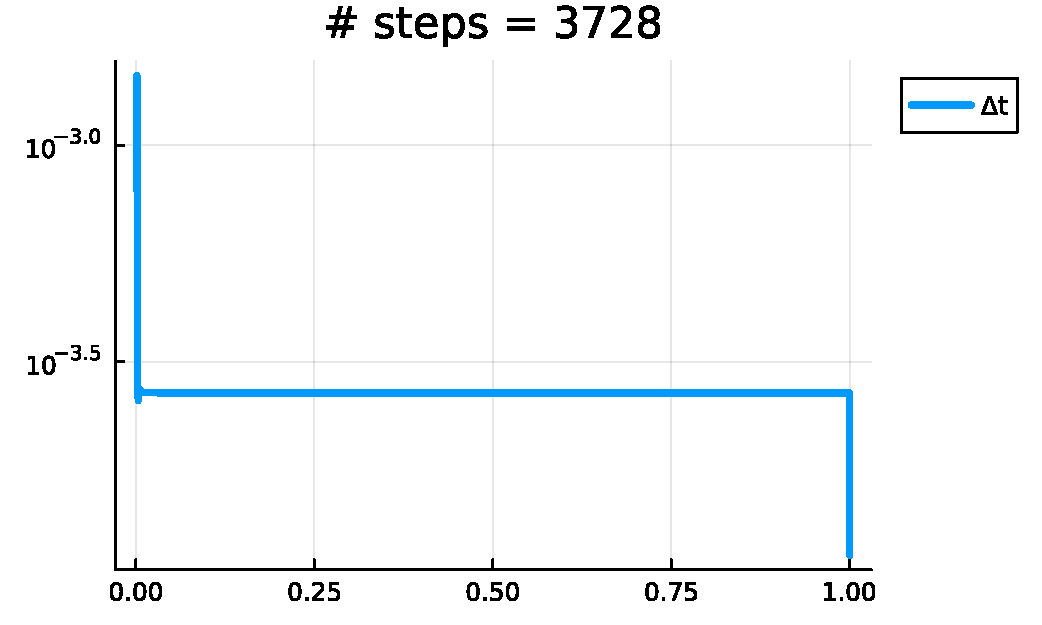
\includegraphics[width=\linewidth]{/figures/Chapter5_26_1.pdf}

\begin{lstlisting}
(*@\HLJLn{soln}@*) (*@\HLJLoB{=}@*)  (*@\HLJLnf{solve}@*)(*@\HLJLp{(}@*)(*@\HLJLn{prob}@*)(*@\HLJLp{,}@*) (*@\HLJLnf{Rodas4}@*)(*@\HLJLp{(),}@*)(*@\HLJLn{abstol}@*)(*@\HLJLoB{=}@*)(*@\HLJLnfB{1e-4}@*)(*@\HLJLp{);}@*)
(*@\HLJLn{tv}@*) (*@\HLJLoB{=}@*) (*@\HLJLn{soln}@*)(*@\HLJLoB{.}@*)(*@\HLJLn{t}@*)
(*@\HLJLn{nt}@*) (*@\HLJLoB{=}@*) (*@\HLJLnf{length}@*)(*@\HLJLp{(}@*)(*@\HLJLn{tv}@*)(*@\HLJLp{)}@*)
\end{lstlisting}

\begin{lstlisting}
22
\end{lstlisting}


\begin{lstlisting}
(*@\HLJLn{errs}@*) (*@\HLJLoB{=}@*) (*@\HLJLnf{zeros}@*)(*@\HLJLp{(}@*)(*@\HLJLn{nt}@*)(*@\HLJLoB{-}@*)(*@\HLJLni{1}@*)(*@\HLJLp{)}@*)
(*@\HLJLk{for}@*) (*@\HLJLn{i}@*) (*@\HLJLoB{=}@*) (*@\HLJLni{2}@*)(*@\HLJLoB{:}@*)(*@\HLJLn{nt}@*)
    (*@\HLJLn{errs}@*)(*@\HLJLp{[}@*)(*@\HLJLn{i}@*)(*@\HLJLoB{-}@*)(*@\HLJLni{1}@*)(*@\HLJLp{]}@*) (*@\HLJLoB{=}@*) (*@\HLJLnf{norm}@*)(*@\HLJLp{(}@*)(*@\HLJLn{ue}@*)(*@\HLJLoB{.}@*)(*@\HLJLp{(}@*)(*@\HLJLn{x}@*)(*@\HLJLp{[}@*)(*@\HLJLni{2}@*)(*@\HLJLoB{:}@*)(*@\HLJLn{nx}@*)(*@\HLJLoB{+}@*)(*@\HLJLni{1}@*)(*@\HLJLp{],}@*)(*@\HLJLn{tv}@*)(*@\HLJLp{[}@*)(*@\HLJLn{i}@*)(*@\HLJLp{])}@*) (*@\HLJLoB{-}@*) (*@\HLJLn{soln}@*)(*@\HLJLoB{.}@*)(*@\HLJLn{u}@*)(*@\HLJLp{[}@*)(*@\HLJLn{i}@*)(*@\HLJLp{],}@*)(*@\HLJLn{Inf}@*)(*@\HLJLp{)}@*)
(*@\HLJLk{end}@*)
(*@\HLJLnf{norm}@*)(*@\HLJLp{(}@*)(*@\HLJLn{errs}@*)(*@\HLJLp{,}@*)(*@\HLJLn{Inf}@*)(*@\HLJLp{)}@*)
\end{lstlisting}

\begin{lstlisting}
0.00023693854401607428
\end{lstlisting}


\begin{lstlisting}
(*@\HLJLcs{{\#}}@*) (*@\HLJLcs{Let{\textquotesingle}s}@*) (*@\HLJLcs{analyze}@*) (*@\HLJLcs{the}@*) (*@\HLJLcs{numerical}@*) (*@\HLJLcs{solution}@*) (*@\HLJLcs{a}@*) (*@\HLJLcs{bit...}@*)
(*@\HLJLn{dt}@*) (*@\HLJLoB{=}@*) (*@\HLJLnf{diff}@*)(*@\HLJLp{(}@*)(*@\HLJLn{soln}@*)(*@\HLJLoB{.}@*)(*@\HLJLn{t}@*)(*@\HLJLp{)}@*)
(*@\HLJLn{plt1}@*) (*@\HLJLoB{=}@*) (*@\HLJLnf{plot}@*)(*@\HLJLp{(}@*)(*@\HLJLn{soln}@*)(*@\HLJLoB{.}@*)(*@\HLJLn{t}@*)(*@\HLJLp{[}@*)(*@\HLJLni{2}@*)(*@\HLJLoB{:}@*)(*@\HLJLk{end}@*)(*@\HLJLp{],}@*) (*@\HLJLn{dt}@*)(*@\HLJLp{,}@*) (*@\HLJLn{yscale}@*) (*@\HLJLoB{=}@*) (*@\HLJLsc{:log10}@*)(*@\HLJLp{,}@*) (*@\HLJLn{size}@*) (*@\HLJLoB{=}@*) (*@\HLJLp{(}@*)(*@\HLJLni{500}@*)(*@\HLJLp{,}@*) (*@\HLJLni{300}@*)(*@\HLJLp{),}@*) (*@\HLJLn{lw}@*) (*@\HLJLoB{=}@*) (*@\HLJLni{3}@*)(*@\HLJLp{,}@*) (*@\HLJLn{label}@*) (*@\HLJLoB{=}@*) (*@\HLJLs{"{}\ensuremath{\Delta}t"{}}@*)(*@\HLJLp{,}@*) 
     (*@\HLJLn{legend}@*) (*@\HLJLoB{=}@*) (*@\HLJLsc{:outertopright}@*)(*@\HLJLp{,}@*) (*@\HLJLn{title}@*) (*@\HLJLoB{=}@*) (*@\HLJLs{"{}{\#}}@*) (*@\HLJLs{steps}@*) (*@\HLJLs{=}@*) (*@\HLJLsi{{\$}}@*)(*@\HLJLp{(}@*)(*@\HLJLnf{length}@*)(*@\HLJLp{(}@*)(*@\HLJLn{soln}@*)(*@\HLJLoB{.}@*)(*@\HLJLn{t}@*)(*@\HLJLp{))}@*)(*@\HLJLs{"{}}@*)(*@\HLJLp{)}@*)
\end{lstlisting}

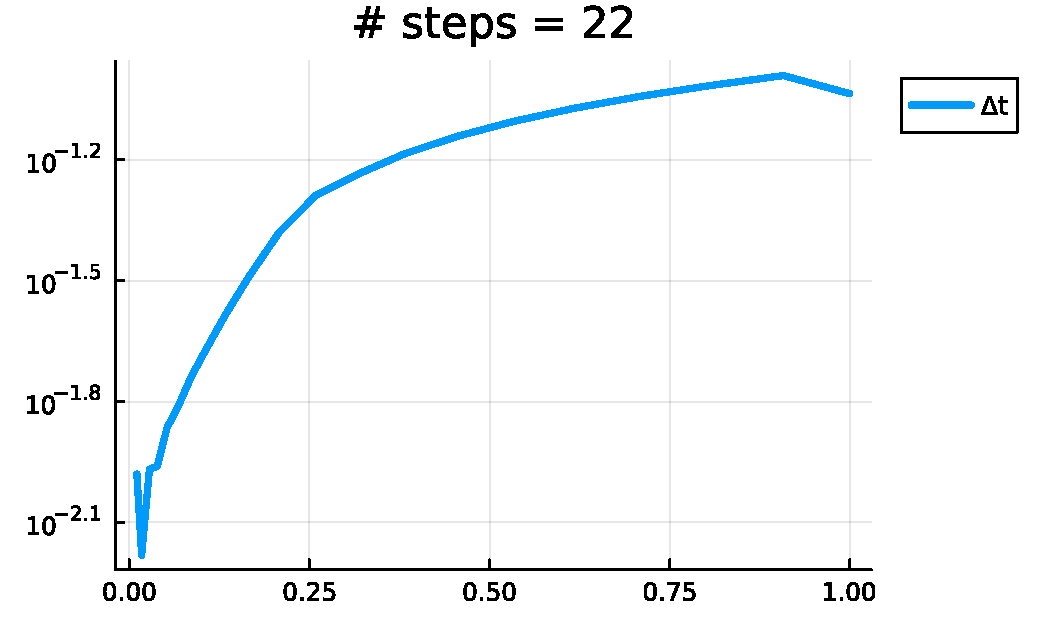
\includegraphics[width=\linewidth]{/figures/Chapter5_29_1.pdf}

\subsection{Spectral methods for the diffusion equation}
In the previous sections, we used finite differences (studied in Chapter 1) to approximate the solution to the diffusion equation. Here we use the approximation methods we studied in Chapters 2-4 (Fourier methods, Chebyshev methods, orthogonal polynomial methods) to design spectral methods for the diffusion equation.

\subsubsection{Fourier spectral method}
Let's briefly recall some facts from Chapter 2: the trigonometric interpolant

\[
f(s) \approx p_n(s) = \sum_{k=-m}^{m}\tilde{c}^n_k {\rm e}^{{\rm i}ks}, \qquad n = 2m + 1, 
\]
interpolates $f$ at the following evenly spaced points on the interval $[0, 2\pi)$:

\[
s_j = j h,\qquad j = 0, \ldots, n-1, \qquad h = \frac{2\pi}{n}
\]
and the approximate Fourier coefficients

\[
\tilde{c}^n_k   =\frac{1}{n}\sum_{j = 0}^{n-1} f(s_j)\mathrm{e}^{-\mathrm{i}ks_j} 
\]
can be computed with the FFT.

Let's return to the diffusion equation $u_t = u_{xx}$ for $(x,t) \in (0,1)\times(0,T]$ subject to the following initial and boundary data:

\[
u(x,0) = f(x), \qquad x \in [0, 1], \qquad u(0,t) = \varphi_0(t), \qquad u(1,t) = \varphi_1(t).
\]
Since $x \in [0, 1]$ and $s \in [0, 2\pi]$, the variables are related according to $s = 2\pi x$.

Let's approximate the solution to the diffusion equation for each $t \in [0, T]$ by a trigonometric interpolant in $x$: 

\[
u(x,t) \approx u_n(x,t) = \sum_{k=-m}^{m} \tilde{u}_k(t) {\rm e}^{2\pi{\rm i}kx}.
\]
We have that

\[
\frac{\partial}{\partial t}u(x,t) \approx \frac{\partial}{\partial t} u_n(x,t) = \sum_{k=-m}^{m} \tilde{u}_k'(t) {\rm e}^{2\pi{\rm i}kx}
\]
and

\[
\frac{\partial^2}{\partial x^2}u(x,t) \approx \frac{\partial^2}{\partial x^2} u_n(x,t) = -4\pi^2\sum_{k=-m}^{m} k^2\tilde{u}_k(t) {\rm e}^{2\pi{\rm i}kx}.
\]
We require that $u_n(x,t)$ satisfy the diffusion equation, which implies that

\[
\tilde{u}_k'(t)  = -4\pi^2 k^2 \tilde{u}_k(t), \qquad k = -m, \ldots, m.
\]
This is a diagonal system of ODEs, which has the solution

\[
\tilde{u}_k(t) = {\rm e}^{-4\pi^2 k^2 t}\tilde{u}_k(0), \qquad k = -m, \ldots, m.
\]
We can compute $\tilde{u}_k(0)$ with the FFT by requiring that $u_n(x,0)$ interpolates $u(x,0) = f(x)$ at equally spaced points:

\[
u(x_j,0) = f(x_j) = u_n(x_j,0) = \sum_{k=-m}^{m} \tilde{u}_k(0) {\rm e}^{2\pi{\rm i}x_j}, \qquad x_j = \frac{j}{n}, \qquad j = 0, \ldots, n-1.
\]
We also require that the boundary conditions be satisfied:

\[
u(0,t) = \varphi_0(t) = u_n(0,t) = \sum_{k=-m}^{m}\tilde{u}_k(t) = \sum_{k=-m}^{m}{\rm e}^{-4\pi^2 k^2 t}\tilde{u}_k(0)
\]
and

\[
u(1,t) = \varphi_1(t) = u_n(1,t) = \sum_{k=-m}^{m}\tilde{u}_k(t) = \sum_{k=-m}^{m}{\rm e}^{-4\pi^2 k^2 t}\tilde{u}_k(0).
\]
These conditions cannot be satsfied unless $u(0,t) = u(1,t)$, i.e., unless periodic boundary conditions are specified, in which case the approximate solution is

\[
u_n(x,t) = \sum_{k=-m}^{m}  {\rm e}^{2\pi{\rm i}kx-4\pi^2 k^2 t} \tilde{u}_k(0)
\]
and the exact solution is

\[
u(x,t) = \sum_{k=-\infty}^{\infty}  {\rm e}^{2\pi{\rm i}kx-4\pi^2 k^2 t} u_k(0)
\]
where

\[
u(x,0) = f(x) = \sum_{k=-\infty}^{\infty}u_k(0) {\rm e}^{2\pi{\rm i}kx },
\]
that is,

\[
u_k(0) = \int_{0}^{1} f(x){\rm e}^{-2\pi{\rm i}kx}\,{\rm d}x.
\]
Notice that the Fourier spectral method is a "coefficient space" method because we re-formulated the PDE problem as a system of ODEs satisfied by the (approximate) Fourier coefficients of the solution.  We'll now consider a "value space" method.  

\subsubsection{Fourier collocation method (Fourier pseudospectral method)}
Let's again recall some facts from Chapter 2: the value space representation of the $2\pi$-periodic trigonometric interpolant is

\[
p_n(s) = \sum_{k=0}^{n-1}\ell_0(s-s_k)f(s_k), 
\]
where $n$ is odd with $n = 2m + 1$, the $s_k$ are evenly spaced points on the interval $[0, 2\pi)$ and

\[
\ell_0(s) = \begin{cases}
\displaystyle{\frac{1}{n}\frac{\sin((m+1/2)s)}{\sin(s/2)}} & \text{if } s \neq 0, \pm 2\pi, \pm 4\pi, \ldots \\
1 & \text{otherwise}
\end{cases}.
\]
Since the basis functions $\ell_0(s-s_k)$ have the periodic delta interpolation property, namely

\[
\ell_0(s_j-s_k) = \begin{cases}
1 & \text{if } j = k, k \pm n, k \pm 2n, \ldots \\
0 & \text{otherwise}
\end{cases}
\]
it follows that $p_n(s_j) = f(s_j)$, $j = 0, \ldots, n-1$, where the points $s_j$ are evenly spaced on the interval $[0, 2\pi)$.

We can use this interpolant to approximate the solution to the diffusion equation on $(x,t) \in (0,1)\times (0, T]$ as follows: 

\[
u(x,t) \approx u_n(x,t) = \sum_{k=0}^{n-1}\ell_0(2\pi (x- x_k))v_k(t), \qquad x_k = \frac{k}{n},
\]
where, from the periodic delta interpolation property,

\[
u(x_j,t) \approx u_n(x_j,t) = v_j(t), \qquad j = 0, \ldots, n-1.
\]
We require that $u_n(x,t)$ satisfies the diffusion equation at the points $x_j$ (known as the collocation points). We have that

\[
\frac{\partial}{\partial t}u_n(x_j,t) = v_j'(t), \qquad j = 0, \ldots, n-1,
\]
and

\[
\frac{\partial^2}{\partial x^2}u_n(x_j,t) = 4\pi^2 \sum_{k=0}^{n-1}\ell_0''(2\pi (x_j- x_k))v_k(t).
\]
From the initial data, we have that

\[
u(x_j,0) = f(x_j) = u_n(x_j,0) = v_j(0), \qquad j = 0, \ldots, n-1,
\]
and from the boundary data,

\[
u(0,t) = \varphi_0(t) = u_n(0,t) = v_0(t)
\]
and because $u_n(x,t)$ is $1$-periodic in $x$,

\[
u(1,t) = \varphi_1(t) = u_n(1,t) = v_0(t),
\]
which can only be satisfied if

\[
u(1,t) = u(0,t)
\]
i.e., if periodic boundary conditions are imposed.

Hence a Fourier pseudospectral / Fourier collocation method for the diffusion equation with periodic boundary conditions is

\[
\mathbf{v}'(t) = D_2 \mathbf{v}(t)
\]
where

\[
\mathbf{v}(t) = \begin{bmatrix}
v_0(t) \\
\vdots \\
v_{n-1}(t)
\end{bmatrix}
\]
and the entries of the second-order differentiation matrix $D_2$ are


\begin{eqnarray*}
\left(D_2\right)_{j,k} &=& 4\pi^2\ell_0''(2\pi (x_j- x_k)) \\
&=& \begin{cases}
-\frac{\pi^2}{3}\left(n^2 - 1    \right)  & \text{if } j = k\\
\displaystyle{2\pi^2(-1)^{j-k+1}\frac{\cos [\pi (j-k)/n] }{ \sin^2 [\pi (j-k)/n] }} & \text{if } j \neq k
\end{cases}
\end{eqnarray*}
for $j,k = 0, \ldots, n-1$.

Let's check this:


\begin{lstlisting}
(*@\HLJLn{n}@*) (*@\HLJLoB{=}@*) (*@\HLJLni{29}@*)
(*@\HLJLnf{D2m}@*)(*@\HLJLp{(}@*)(*@\HLJLn{n}@*)(*@\HLJLp{)}@*) (*@\HLJLoB{=}@*) (*@\HLJLp{[}@*)(*@\HLJLn{j}@*) (*@\HLJLoB{==}@*) (*@\HLJLn{k}@*) (*@\HLJLoB{?}@*) 
    (*@\HLJLoB{-}@*)(*@\HLJLn{\ensuremath{\pi}}@*)(*@\HLJLoB{{\textasciicircum}}@*)(*@\HLJLni{2}@*)(*@\HLJLoB{/}@*)(*@\HLJLni{3}@*)(*@\HLJLoB{*}@*)(*@\HLJLp{(}@*)(*@\HLJLn{n}@*)(*@\HLJLoB{{\textasciicircum}}@*)(*@\HLJLni{2}@*) (*@\HLJLoB{-}@*) (*@\HLJLni{1}@*)(*@\HLJLp{)}@*) (*@\HLJLoB{:}@*) 
    (*@\HLJLni{2}@*)(*@\HLJLn{\ensuremath{\pi}}@*)(*@\HLJLoB{{\textasciicircum}}@*)(*@\HLJLni{2}@*)(*@\HLJLoB{*}@*)(*@\HLJLp{(}@*)(*@\HLJLoB{-}@*)(*@\HLJLni{1}@*)(*@\HLJLp{)}@*)(*@\HLJLoB{{\textasciicircum}}@*)(*@\HLJLp{(}@*)(*@\HLJLn{j}@*)(*@\HLJLoB{-}@*)(*@\HLJLn{k}@*)(*@\HLJLoB{+}@*)(*@\HLJLni{1}@*)(*@\HLJLp{)}@*)(*@\HLJLoB{*}@*)(*@\HLJLnf{cos}@*)(*@\HLJLp{(}@*)(*@\HLJLn{\ensuremath{\pi}}@*)(*@\HLJLoB{*}@*)(*@\HLJLp{(}@*)(*@\HLJLn{j}@*)(*@\HLJLoB{-}@*)(*@\HLJLn{k}@*)(*@\HLJLp{)}@*)(*@\HLJLoB{/}@*)(*@\HLJLn{n}@*)(*@\HLJLp{)}@*)(*@\HLJLoB{/}@*)(*@\HLJLp{(}@*)(*@\HLJLnf{sin}@*)(*@\HLJLp{(}@*)(*@\HLJLn{\ensuremath{\pi}}@*)(*@\HLJLoB{*}@*)(*@\HLJLp{(}@*)(*@\HLJLn{j}@*)(*@\HLJLoB{-}@*)(*@\HLJLn{k}@*)(*@\HLJLp{)}@*)(*@\HLJLoB{/}@*)(*@\HLJLn{n}@*)(*@\HLJLp{))}@*)(*@\HLJLoB{{\textasciicircum}}@*)(*@\HLJLni{2}@*) 
    (*@\HLJLk{for}@*) (*@\HLJLn{j}@*) (*@\HLJLoB{=}@*) (*@\HLJLni{0}@*)(*@\HLJLoB{:}@*)(*@\HLJLn{n}@*)(*@\HLJLoB{-}@*)(*@\HLJLni{1}@*)(*@\HLJLp{,}@*) (*@\HLJLn{k}@*) (*@\HLJLoB{=}@*) (*@\HLJLni{0}@*)(*@\HLJLoB{:}@*)(*@\HLJLn{n}@*)(*@\HLJLoB{-}@*)(*@\HLJLni{1}@*)(*@\HLJLp{]}@*)
(*@\HLJLn{f}@*) (*@\HLJLoB{=}@*) (*@\HLJLn{x}@*) (*@\HLJLoB{->}@*) (*@\HLJLnf{exp}@*)(*@\HLJLp{(}@*)(*@\HLJLnf{sin}@*)(*@\HLJLp{(}@*)(*@\HLJLni{2}@*)(*@\HLJLn{\ensuremath{\pi}}@*)(*@\HLJLoB{*}@*)(*@\HLJLn{x}@*)(*@\HLJLp{))}@*)
(*@\HLJLn{df}@*) (*@\HLJLoB{=}@*) (*@\HLJLn{x}@*) (*@\HLJLoB{->}@*) (*@\HLJLnf{f}@*)(*@\HLJLp{(}@*)(*@\HLJLn{x}@*)(*@\HLJLp{)}@*)(*@\HLJLoB{*}@*)(*@\HLJLni{2}@*)(*@\HLJLn{\ensuremath{\pi}}@*)(*@\HLJLoB{*}@*)(*@\HLJLnf{cos}@*)(*@\HLJLp{(}@*)(*@\HLJLni{2}@*)(*@\HLJLn{\ensuremath{\pi}}@*)(*@\HLJLoB{*}@*)(*@\HLJLn{x}@*)(*@\HLJLp{)}@*)
(*@\HLJLn{d2f}@*) (*@\HLJLoB{=}@*) (*@\HLJLn{x}@*) (*@\HLJLoB{->}@*) (*@\HLJLnf{f}@*)(*@\HLJLp{(}@*)(*@\HLJLn{x}@*)(*@\HLJLp{)}@*)(*@\HLJLoB{*}@*)(*@\HLJLp{(}@*)(*@\HLJLni{2}@*)(*@\HLJLn{\ensuremath{\pi}}@*)(*@\HLJLoB{*}@*)(*@\HLJLnf{cos}@*)(*@\HLJLp{(}@*)(*@\HLJLni{2}@*)(*@\HLJLn{\ensuremath{\pi}}@*)(*@\HLJLoB{*}@*)(*@\HLJLn{x}@*)(*@\HLJLp{))}@*)(*@\HLJLoB{{\textasciicircum}}@*)(*@\HLJLni{2}@*) (*@\HLJLoB{-}@*) (*@\HLJLni{4}@*)(*@\HLJLn{\ensuremath{\pi}}@*)(*@\HLJLoB{{\textasciicircum}}@*)(*@\HLJLni{2}@*)(*@\HLJLoB{*}@*)(*@\HLJLnf{f}@*)(*@\HLJLp{(}@*)(*@\HLJLn{x}@*)(*@\HLJLp{)}@*)(*@\HLJLoB{*}@*)(*@\HLJLnf{sin}@*)(*@\HLJLp{(}@*)(*@\HLJLni{2}@*)(*@\HLJLn{\ensuremath{\pi}}@*)(*@\HLJLoB{*}@*)(*@\HLJLn{x}@*)(*@\HLJLp{)}@*)
(*@\HLJLn{xx}@*) (*@\HLJLoB{=}@*) (*@\HLJLnf{range}@*)(*@\HLJLp{(}@*)(*@\HLJLni{0}@*)(*@\HLJLp{,}@*)(*@\HLJLni{1}@*)(*@\HLJLp{,}@*)(*@\HLJLn{n}@*)(*@\HLJLoB{+}@*)(*@\HLJLni{1}@*)(*@\HLJLp{)[}@*)(*@\HLJLni{1}@*)(*@\HLJLoB{:}@*)(*@\HLJLk{end}@*)(*@\HLJLoB{-}@*)(*@\HLJLni{1}@*)(*@\HLJLp{]}@*)
(*@\HLJLnf{norm}@*)(*@\HLJLp{(}@*)(*@\HLJLn{d2f}@*)(*@\HLJLoB{.}@*)(*@\HLJLp{(}@*)(*@\HLJLn{xx}@*)(*@\HLJLp{)}@*) (*@\HLJLoB{-}@*) (*@\HLJLnf{D2m}@*)(*@\HLJLp{(}@*)(*@\HLJLn{n}@*)(*@\HLJLp{)}@*)(*@\HLJLoB{*}@*)(*@\HLJLn{f}@*)(*@\HLJLoB{.}@*)(*@\HLJLp{(}@*)(*@\HLJLn{xx}@*)(*@\HLJLp{),}@*) (*@\HLJLn{Inf}@*)(*@\HLJLp{)}@*)
\end{lstlisting}

\begin{lstlisting}
4.078515303262975e-12
\end{lstlisting}


The differentiation matrix $D_2$ is a normal matrix because it is symmetric:


\begin{lstlisting}
(*@\HLJLnf{D2m}@*)(*@\HLJLp{(}@*)(*@\HLJLni{5}@*)(*@\HLJLp{)}@*)
\end{lstlisting}

\begin{lstlisting}
5(*@\ensuremath{\times}@*)5 Matrix(*@{{\{}}@*)Float64(*@{{\}}}@*):
 -78.9568    46.2221    -6.74372   -6.74372   46.2221
  46.2221   -78.9568    46.2221    -6.74372   -6.74372
  -6.74372   46.2221   -78.9568    46.2221    -6.74372
  -6.74372   -6.74372   46.2221   -78.9568    46.2221
  46.2221    -6.74372   -6.74372   46.2221   -78.9568
\end{lstlisting}


From the results we proved above, to show that the semi-discrete method $\mathbf{v}'(t) = D_2 \mathbf{v}(t)$ is stable, we need to prove that the real part of the eigenvalues of $D_2 \in \mathbb{R}^{n \times n}$ are bounded above as $n \to \infty$.  To find the eigenvalues of $D_2$, we'll use some facts we learned in Chapter 2 to find its eigendecomposition (spectral factorisation) using the FFT.

The matrix $D_2$ is also circulant and all circulant matrices can be diagonalised with the FFT matrix, as we'll see shortly, which also implies that matrix-vector multiplication with a circulant marix can be computed with the FFT.

Recall that we showed that derivates can be computed with the FFT instead of differentiation matrices:


\begin{lstlisting}
(*@\HLJLn{m}@*) (*@\HLJLoB{=}@*) (*@\HLJLp{(}@*)(*@\HLJLn{n}@*)(*@\HLJLoB{-}@*)(*@\HLJLni{1}@*)(*@\HLJLp{)}@*)(*@\HLJLoB{\ensuremath{\div}}@*)(*@\HLJLni{2}@*)
(*@\HLJLnf{norm}@*)(*@\HLJLp{(}@*)(*@\HLJLn{d2f}@*)(*@\HLJLoB{.}@*)(*@\HLJLp{(}@*)(*@\HLJLn{xx}@*)(*@\HLJLp{)}@*) (*@\HLJLoB{-}@*) (*@\HLJLnf{ifft}@*)(*@\HLJLp{(}@*)(*@\HLJLnf{ifftshift}@*)(*@\HLJLp{(}@*)(*@\HLJLoB{-}@*)(*@\HLJLni{4}@*)(*@\HLJLn{\ensuremath{\pi}}@*)(*@\HLJLoB{{\textasciicircum}}@*)(*@\HLJLni{2}@*)(*@\HLJLoB{*}@*)(*@\HLJLp{(}@*)(*@\HLJLoB{-}@*)(*@\HLJLn{m}@*)(*@\HLJLoB{:}@*)(*@\HLJLn{m}@*)(*@\HLJLp{)}@*)(*@\HLJLoB{.{\textasciicircum}}@*)(*@\HLJLni{2}@*)(*@\HLJLp{)}@*) (*@\HLJLoB{.*}@*)(*@\HLJLnf{fft}@*)(*@\HLJLp{(}@*)(*@\HLJLn{f}@*)(*@\HLJLoB{.}@*)(*@\HLJLp{(}@*)(*@\HLJLn{xx}@*)(*@\HLJLp{))),}@*) (*@\HLJLn{Inf}@*)(*@\HLJLp{)}@*)
\end{lstlisting}

\begin{lstlisting}
1.5347723092418164e-12
\end{lstlisting}


We also learned that the FFT is equivalent to a certain matrix-vector multiplication.  That is, the FFT applied to a vector $\mathbf{f}$ performs the matrix-vector multiplication $Q_n \mathbf{f}$, where $Q_n$ is an $n\times n$ unitary matrix that was defined in Chapter 2. Here is a reminder of the matrix $Q_n$:


\begin{lstlisting}
(*@\HLJLnf{Qm}@*)(*@\HLJLp{(}@*)(*@\HLJLn{n}@*)(*@\HLJLp{)}@*) (*@\HLJLoB{=}@*) (*@\HLJLp{[}@*)(*@\HLJLnf{exp}@*)(*@\HLJLp{(}@*)(*@\HLJLoB{-}@*)(*@\HLJLni{2}@*)(*@\HLJLn{\ensuremath{\pi}}@*)(*@\HLJLoB{*}@*)(*@\HLJLn{im}@*)(*@\HLJLoB{*}@*)(*@\HLJLp{(}@*)(*@\HLJLn{k}@*)(*@\HLJLoB{-}@*)(*@\HLJLni{1}@*)(*@\HLJLp{)}@*)(*@\HLJLoB{*}@*)(*@\HLJLn{j}@*)(*@\HLJLoB{/}@*)(*@\HLJLn{n}@*)(*@\HLJLp{)}@*) (*@\HLJLk{for}@*) (*@\HLJLn{k}@*) (*@\HLJLoB{=}@*) (*@\HLJLni{1}@*)(*@\HLJLoB{:}@*)(*@\HLJLn{n}@*)(*@\HLJLp{,}@*) (*@\HLJLn{j}@*)(*@\HLJLoB{=}@*)(*@\HLJLni{1}@*)(*@\HLJLoB{:}@*)(*@\HLJLn{n}@*)(*@\HLJLp{]}@*)(*@\HLJLoB{/}@*)(*@\HLJLnf{sqrt}@*)(*@\HLJLp{(}@*)(*@\HLJLn{n}@*)(*@\HLJLp{)}@*)
(*@\HLJLn{n}@*) (*@\HLJLoB{=}@*) (*@\HLJLni{5}@*)
(*@\HLJLnf{Qm}@*)(*@\HLJLp{(}@*)(*@\HLJLni{5}@*)(*@\HLJLp{)}@*)(*@\HLJLoB{{\textquotesingle}*}@*)(*@\HLJLnf{Qm}@*)(*@\HLJLp{(}@*)(*@\HLJLni{5}@*)(*@\HLJLp{)}@*) (*@\HLJLoB{\ensuremath{\approx}}@*) (*@\HLJLn{I}@*)
\end{lstlisting}

\begin{lstlisting}
true
\end{lstlisting}


We also learned that the $ifftshift$ command is equivalent to multiplication by a permutation matrix $P$, where

\[
P = \left(
\begin{array}{c c}
   & I_{m} \\
I_{m+1} & 
\end{array}
\right).
\]
From the results of Chapter 2, it follows that the command $ifft(ifftshift(-(-m:m).^2)fft(f(xx)))$ used above for approximating the second derivative on an equispaced grid is equivalent to multipilication by the matrix

\[
Q_n^*P^*\Lambda PQ_n, \qquad \Lambda = -4\pi^2\mathrm{diag}(m^2, (m-1)^2, \ldots, 0, 1^2, \ldots, m^2),
\]
and moreover

\[
D_2 = Q_n^*P^*\Lambda PQ_n.
\]
Let's check this:


\begin{lstlisting}
(*@\HLJLn{n}@*) (*@\HLJLoB{=}@*) (*@\HLJLni{11}@*)
(*@\HLJLn{m}@*) (*@\HLJLoB{=}@*) (*@\HLJLp{(}@*)(*@\HLJLn{n}@*)(*@\HLJLoB{-}@*)(*@\HLJLni{1}@*)(*@\HLJLp{)}@*)(*@\HLJLoB{\ensuremath{\div}}@*)(*@\HLJLni{2}@*)
(*@\HLJLn{P}@*) (*@\HLJLoB{=}@*) (*@\HLJLnf{sparse}@*)(*@\HLJLp{(}@*)(*@\HLJLni{1}@*)(*@\HLJLoB{:}@*)(*@\HLJLn{n}@*)(*@\HLJLp{,}@*) (*@\HLJLp{[}@*)(*@\HLJLn{m}@*)(*@\HLJLoB{+}@*)(*@\HLJLni{2}@*)(*@\HLJLoB{:}@*)(*@\HLJLn{n}@*)(*@\HLJLp{;}@*)(*@\HLJLni{1}@*)(*@\HLJLoB{:}@*)(*@\HLJLn{m}@*)(*@\HLJLoB{+}@*)(*@\HLJLni{1}@*)(*@\HLJLp{],}@*) (*@\HLJLnf{fill}@*)(*@\HLJLp{(}@*)(*@\HLJLni{1}@*)(*@\HLJLp{,}@*)(*@\HLJLn{n}@*)(*@\HLJLp{))}@*)
(*@\HLJLn{Q}@*) (*@\HLJLoB{=}@*) (*@\HLJLnf{Qm}@*)(*@\HLJLp{(}@*)(*@\HLJLn{n}@*)(*@\HLJLp{)}@*)
(*@\HLJLn{D2}@*) (*@\HLJLoB{=}@*) (*@\HLJLnf{D2m}@*)(*@\HLJLp{(}@*)(*@\HLJLn{n}@*)(*@\HLJLp{)}@*)
(*@\HLJLoB{-}@*)(*@\HLJLni{4}@*)(*@\HLJLn{\ensuremath{\pi}}@*)(*@\HLJLoB{{\textasciicircum}}@*)(*@\HLJLni{2}@*)(*@\HLJLoB{*}@*)(*@\HLJLn{Q}@*)(*@\HLJLoB{{\textquotesingle}*}@*)(*@\HLJLn{P}@*)(*@\HLJLoB{{\textquotesingle}}@*)(*@\HLJLnf{diagm}@*)(*@\HLJLp{((}@*)(*@\HLJLoB{-}@*)(*@\HLJLn{m}@*)(*@\HLJLoB{:}@*)(*@\HLJLn{m}@*)(*@\HLJLp{)}@*)(*@\HLJLoB{.{\textasciicircum}}@*)(*@\HLJLni{2}@*)(*@\HLJLp{)}@*)(*@\HLJLoB{*}@*)(*@\HLJLn{P}@*)(*@\HLJLoB{*}@*)(*@\HLJLn{Q}@*) (*@\HLJLoB{\ensuremath{\approx}}@*) (*@\HLJLn{D2}@*)
\end{lstlisting}

\begin{lstlisting}
true
\end{lstlisting}


This is the spectral factorisation of $D_2$ and it shows that its eigenvalues are $-4\pi^2k^2$ for $k = 0, \ldots, m$.  Since the eigenvalues are bounded above by $0$, we conclude that the Fourier pseudospectral / Fourier collocation semidiscrete method $\mathbf{v}' = D_2\mathbf{v}$ is stable.  If the solution to the diffusion equation is continuous and $1$-periodic, then we know from Chapter 2 that the trigonometric interpolant will converge (for a fixed time $t$) to the exact solution as $n \to \infty$, hence the method is consistent and therefore (by the Lax equivalence theorem) convergent.

If we were to use Euler's method for time stepping, then the step size restriction would be

\[
\tau \leq \frac{2}{\rho(A)} = \frac{1}{2\pi^2 m^2} = \frac{2}{\pi^2 (n-1)^2}.
\]

\begin{lstlisting}
(*@\HLJLn{n}@*) (*@\HLJLoB{=}@*) (*@\HLJLni{91}@*)
(*@\HLJLn{m}@*) (*@\HLJLoB{=}@*) (*@\HLJLp{(}@*)(*@\HLJLn{n}@*)(*@\HLJLoB{-}@*)(*@\HLJLni{1}@*)(*@\HLJLp{)}@*)(*@\HLJLoB{\ensuremath{\div}}@*)(*@\HLJLni{2}@*)
(*@\HLJLn{f}@*) (*@\HLJLoB{=}@*) (*@\HLJLn{x}@*) (*@\HLJLoB{->}@*) (*@\HLJLnf{sin}@*)(*@\HLJLp{(}@*)(*@\HLJLn{\ensuremath{\pi}}@*)(*@\HLJLoB{*}@*)(*@\HLJLn{x}@*)(*@\HLJLoB{/}@*)(*@\HLJLni{2}@*)(*@\HLJLp{)}@*) (*@\HLJLoB{+}@*) (*@\HLJLnfB{0.5}@*)(*@\HLJLoB{*}@*)(*@\HLJLnf{sin}@*)(*@\HLJLp{(}@*)(*@\HLJLni{2}@*)(*@\HLJLn{\ensuremath{\pi}}@*)(*@\HLJLoB{*}@*)(*@\HLJLn{x}@*)(*@\HLJLp{)}@*)
(*@\HLJLn{T}@*) (*@\HLJLoB{=}@*) (*@\HLJLnfB{0.01}@*)
(*@\HLJLn{F}@*) (*@\HLJLoB{=}@*) (*@\HLJLp{(}@*)(*@\HLJLn{v}@*)(*@\HLJLp{,}@*)(*@\HLJLn{p}@*)(*@\HLJLp{,}@*)(*@\HLJLn{t}@*)(*@\HLJLp{)}@*) (*@\HLJLoB{->}@*) (*@\HLJLnf{real}@*)(*@\HLJLp{(}@*)(*@\HLJLnf{ifft}@*)(*@\HLJLp{(}@*)(*@\HLJLnf{ifftshift}@*)(*@\HLJLp{(}@*)(*@\HLJLoB{-}@*)(*@\HLJLni{4}@*)(*@\HLJLn{\ensuremath{\pi}}@*)(*@\HLJLoB{{\textasciicircum}}@*)(*@\HLJLni{2}@*)(*@\HLJLoB{*}@*)(*@\HLJLp{(}@*)(*@\HLJLoB{-}@*)(*@\HLJLn{m}@*)(*@\HLJLoB{:}@*)(*@\HLJLn{m}@*)(*@\HLJLp{)}@*)(*@\HLJLoB{.{\textasciicircum}}@*)(*@\HLJLni{2}@*)(*@\HLJLp{)}@*) (*@\HLJLoB{.*}@*)(*@\HLJLnf{fft}@*)(*@\HLJLp{(}@*)(*@\HLJLn{v}@*)(*@\HLJLp{)))}@*)
(*@\HLJLn{x}@*) (*@\HLJLoB{=}@*) (*@\HLJLnf{range}@*)(*@\HLJLp{(}@*)(*@\HLJLni{0}@*)(*@\HLJLp{,}@*)(*@\HLJLni{1}@*)(*@\HLJLp{,}@*)(*@\HLJLn{n}@*)(*@\HLJLoB{+}@*)(*@\HLJLni{1}@*)(*@\HLJLp{)[}@*)(*@\HLJLni{1}@*)(*@\HLJLoB{:}@*)(*@\HLJLk{end}@*)(*@\HLJLoB{-}@*)(*@\HLJLni{1}@*)(*@\HLJLp{]}@*)
(*@\HLJLn{prob}@*) (*@\HLJLoB{=}@*) (*@\HLJLnf{ODEProblem}@*)(*@\HLJLp{(}@*)(*@\HLJLn{F}@*)(*@\HLJLp{,}@*) (*@\HLJLn{f}@*)(*@\HLJLoB{.}@*)(*@\HLJLp{(}@*)(*@\HLJLn{x}@*)(*@\HLJLp{),}@*) (*@\HLJLp{(}@*)(*@\HLJLnfB{0.0}@*)(*@\HLJLp{,}@*) (*@\HLJLn{T}@*)(*@\HLJLp{))}@*)
(*@\HLJLn{soln}@*) (*@\HLJLoB{=}@*)  (*@\HLJLnf{solve}@*)(*@\HLJLp{(}@*)(*@\HLJLn{prob}@*)(*@\HLJLp{,}@*)(*@\HLJLnf{RK4}@*)(*@\HLJLp{(),}@*)(*@\HLJLn{abstol}@*)(*@\HLJLoB{=}@*)(*@\HLJLnfB{1e-2}@*)(*@\HLJLp{);}@*)
\end{lstlisting}


In the code above, we used an explicit fourth-order Runge-Kutta method as time stepper / integrator.  Let's compare the maximum step size of the Runge-Kutta method with the step size restriction of Euler's method:


\begin{lstlisting}
(*@\HLJLp{[}@*)(*@\HLJLnf{maximum}@*)(*@\HLJLp{(}@*)(*@\HLJLnf{diff}@*)(*@\HLJLp{(}@*)(*@\HLJLn{soln}@*)(*@\HLJLoB{.}@*)(*@\HLJLn{t}@*)(*@\HLJLp{))}@*) (*@\HLJLni{2}@*)(*@\HLJLoB{/}@*)(*@\HLJLp{(}@*)(*@\HLJLn{\ensuremath{\pi}}@*)(*@\HLJLoB{{\textasciicircum}}@*)(*@\HLJLni{2}@*)(*@\HLJLoB{*}@*)(*@\HLJLp{(}@*)(*@\HLJLn{n}@*)(*@\HLJLoB{-}@*)(*@\HLJLni{1}@*)(*@\HLJLp{)}@*)(*@\HLJLoB{{\textasciicircum}}@*)(*@\HLJLni{2}@*)(*@\HLJLp{)]}@*)
\end{lstlisting}

\begin{lstlisting}
1(*@\ensuremath{\times}@*)2 Matrix(*@{{\{}}@*)Float64(*@{{\}}}@*):
 4.35304e-5  2.50176e-5
\end{lstlisting}


\begin{lstlisting}
(*@\HLJLn{t}@*) (*@\HLJLoB{=}@*) (*@\HLJLn{soln}@*)(*@\HLJLoB{.}@*)(*@\HLJLn{t}@*)
(*@\HLJLn{u}@*) (*@\HLJLoB{=}@*) (*@\HLJLn{soln}@*)(*@\HLJLoB{.}@*)(*@\HLJLn{u}@*)
(*@\HLJLn{nt}@*) (*@\HLJLoB{=}@*) (*@\HLJLnf{length}@*)(*@\HLJLp{(}@*)(*@\HLJLn{soln}@*)(*@\HLJLoB{.}@*)(*@\HLJLn{t}@*)(*@\HLJLp{)}@*)
(*@\HLJLnd{@gif}@*) (*@\HLJLk{for}@*) (*@\HLJLn{i}@*) (*@\HLJLoB{=}@*) (*@\HLJLni{1}@*)(*@\HLJLoB{:}@*)(*@\HLJLn{nt}@*) 
    (*@\HLJLnf{plot}@*)(*@\HLJLp{(}@*)(*@\HLJLn{x}@*)(*@\HLJLp{,}@*) (*@\HLJLn{u}@*)(*@\HLJLp{[}@*)(*@\HLJLni{1}@*)(*@\HLJLp{],}@*) (*@\HLJLn{size}@*) (*@\HLJLoB{=}@*) (*@\HLJLp{(}@*)(*@\HLJLni{700}@*)(*@\HLJLp{,}@*) (*@\HLJLni{150}@*)(*@\HLJLp{),}@*) (*@\HLJLn{label}@*) (*@\HLJLoB{=}@*) (*@\HLJLs{"{}u0"{}}@*)(*@\HLJLp{)}@*)
    (*@\HLJLnf{plot!}@*)(*@\HLJLp{(}@*)(*@\HLJLn{x}@*)(*@\HLJLp{,}@*) (*@\HLJLn{u}@*)(*@\HLJLp{[}@*)(*@\HLJLn{i}@*)(*@\HLJLp{],}@*) (*@\HLJLn{label}@*) (*@\HLJLoB{=}@*) (*@\HLJLs{"{}Fourier}@*) (*@\HLJLs{collocation,t}@*) (*@\HLJLs{=}@*) (*@\HLJLs{"{}}@*) (*@\HLJLoB{*}@*) (*@\HLJLp{(}@*)(*@\HLJLnd{@sprintf}@*)(*@\HLJLp{(}@*)(*@\HLJLs{"{}{\%}.4f"{}}@*)(*@\HLJLp{,}@*) (*@\HLJLn{t}@*)(*@\HLJLp{[}@*)(*@\HLJLn{i}@*)(*@\HLJLp{])),}@*) (*@\HLJLn{legend}@*) (*@\HLJLoB{=}@*) (*@\HLJLsc{:outertopright}@*)(*@\HLJLp{)}@*)
    (*@\HLJLnf{plot!}@*)(*@\HLJLp{(}@*)(*@\HLJLn{x}@*)(*@\HLJLp{,}@*) (*@\HLJLn{ue}@*)(*@\HLJLoB{.}@*)(*@\HLJLp{(}@*)(*@\HLJLn{x}@*)(*@\HLJLp{,}@*)(*@\HLJLn{t}@*)(*@\HLJLp{[}@*)(*@\HLJLn{i}@*)(*@\HLJLp{]),}@*) (*@\HLJLn{label}@*) (*@\HLJLoB{=}@*) (*@\HLJLs{"{}exact}@*) (*@\HLJLs{solution"{}}@*)(*@\HLJLp{)}@*)
(*@\HLJLk{end}@*)
\end{lstlisting}

\begin{lstlisting}
Plots.AnimatedGif((*@{"{}}@*)C:(*@{{\textbackslash}}@*)(*@{{\textbackslash}}@*)Users(*@{{\textbackslash}}@*)(*@{{\textbackslash}}@*)mfaso(*@{{\textbackslash}}@*)(*@{{\textbackslash}}@*)AppData(*@{{\textbackslash}}@*)(*@{{\textbackslash}}@*)Local(*@{{\textbackslash}}@*)(*@{{\textbackslash}}@*)Temp(*@{{\textbackslash}}@*)(*@{{\textbackslash}}@*)jl(*@{{\_}}@*)8uR5DdilQ7.gi
f(*@{"{}}@*))
\end{lstlisting}


Of course, for a problem that doesn't have periodic boundary conditions, Fourier methods won't be accurate.  We saw this in Chapter 2 when we approximated a non-periodic function with a trigonometric interpolant and observed the Gibbs phenomenon. 

\subsubsection{Chebyshev collocation method}
Recall from Chapter 3 the formula for the Lagrange interpolating polynomial at the Chebyshev points:

\[
p_{n}(s) = \sum_{k = 0}^{n}\ell_k(s)f(s_k), \qquad \ell_k(s) = \prod_{\substack{j=0\\ j \neq k}}^{n}\frac{s-s_j}{s_k-s_j}
\]
where the Chebyshev points are

\[
s_k = \cos\left(\frac{\pi k}{n} \right), \qquad k = 0, \ldots, n.
\]
Since we let $s \in [-1, 1]$ and in the diffusion equation we let $x \in [0, 1]$, the variables are related according to

\[
s = 2x - 1,
\]
and we set

\[
x_k = \frac{s_k+1}{2}, \qquad k = 0, \ldots, n.
\]
We approximate the solution to the diffusion equation using an interpolant at the Chebyshev points:

\[
u(x,t) \approx u_n(x,t) = \sum_{k=0}^n \ell_k(2x - 1)v_k(t)
\]
The Lagrange basis polynomials $\ell_k(s)$ have the delta interpolation property,

\[
\ell_k(s_j) = \delta_{j,k} = \begin{cases}
1 & \text{if } k = j \\
0 & \text{otherwise}
\end{cases}
\]
and thus for $j = 0, \ldots, n$

\[
u(x_j,t) \approx u_n(x_j,t)= \sum_{k=0}^n \ell_k(2x_j - 1)v_k(t) = \sum_{k=0}^n \ell_k(s_j)v_k(t) = v_j(t).
\]
The boundary data imply that

\[
u(0,t) = \varphi_0(t) = u_n(0,t) = v_n(t)
\]
and

\[
u(1,t) = \varphi_1(t) = u_n(1,t) = v_0(t)
\]
while the initial data imply

\[
u(x_j,0) = u_n(x_j,0) = f(x_j) = v_j(0), \qquad j = 0, \ldots, n.
\]
We approximate the solution to the diffusion equation by requiring that $u_n(x,t)$ satisfy the diffusion equation at the Chebyshev points (the collocation points). Since

\[
\frac{\partial}{\partial t}u(x_j,t) \approx \frac{\partial}{\partial t} u_n(x_j,t)  = v_j'(t)
\]
and

\[
\frac{\partial^2}{\partial x^2}u(x_j,t) \approx \frac{\partial^2}{\partial x^2} u_n(x_j,t) = 4\sum_{k=0}^n \ell_k''(2x_j - 1)v_k(t) = 4\sum_{k=0}^n \ell_k''(s_j)v_k(t)
\]
we approximate the solution to the diffusion equation as follows


\begin{eqnarray*}
\left(
\begin{array}{c}
v_1'(t) \\
v_2'(t) \\
\vdots \\
v_{n-1}'(t)
\end{array}
\right) &=& 4
\left(
\begin{array}{c c c c c}
\ell''_0(s_1) &\ell''_1(s_1) & \cdots &\ell''_{n-1}(s_1) & \ell''_{n}(s_1) \\
\ell''_0(s_2) &\ell''_1(s_2) & \cdots &\ell''_{n-1}(s_2) & \ell''_{n}(s_2)  \\
     \vdots  & \vdots & \vdots & \vdots & \vdots  \\
\ell''_0(s_{n-1}) &\ell''_1(s_{n-1}) & \cdots &\ell''_{n-1}(s_{n-1}) & \ell''_{n}(s_{n-1})
\end{array} 
\right)
\left(
\begin{array}{c}
v_0(t) \\
v_1(t) \\
\vdots \\
v_{n-1}(t) \\
v_n(t)
\end{array}
\right) \\
&=&4 \left(
\begin{array}{ c c c }
\ell''_1(s_1) & \cdots &\ell''_{n-1}(s_1)  \\
\ell''_1(s_2) & \cdots &\ell''_{n-1}(s_2)   \\
   \vdots & \vdots & \vdots   \\
\ell''_1(s_{n-1}) & \cdots &\ell''_{n-1}(s_{n-1}) 
\end{array} 
\right)
\left(
\begin{array}{c}
v_1(t) \\
\vdots \\
v_{n-1}(t)
\end{array}
\right) \\
& &
+ 4\varphi_1(t)\left(
\begin{array}{c}
\ell''_0(s_1)  \\
\ell''_0(s_2)  \\
     \vdots    \\
\ell''_0(s_{n-1}) 
\end{array} 
\right)
+ 4\varphi_0(t)\left(
\begin{array}{c}
\ell''_n(s_1)  \\
\ell''_n(s_2)  \\
     \vdots    \\
\ell''_n(s_{n-1}) 
\end{array} 
\right)\\
&:=& A \mathbf{v}(t) + \mathbf{h}(t).
\end{eqnarray*}
\paragraph{Spectral factorisation of the second-order Chebyshev differentiation matrix}
Recall from Chapter 3 that the following function builds the (first-order) Chebyshev differentiation matrix, i.e., the  $(n+1) \times (n+1)$ matrix given by

\[
D_1 = \left(
\begin{array}{c c c c}
\ell'_0(s_1) &\ell'_1(s_1) & \cdots  & \ell'_{n}(s_1) \\
\ell'_0(s_2) &\ell'_1(s_2) & \cdots  & \ell'_{n}(s_2)  \\
     \vdots  & \vdots & \vdots &  \vdots  \\
\ell'_0(s_{n-1}) &\ell'_1(s_{n-1}) & \cdots & \ell'_{n}(s_{n-1})
\end{array} 
\right)
\]

\begin{lstlisting}
(*@\HLJLk{function}@*) (*@\HLJLnf{cheb}@*)(*@\HLJLp{(}@*)(*@\HLJLn{n}@*)(*@\HLJLp{)}@*)

    (*@\HLJLn{x}@*) (*@\HLJLoB{=}@*) (*@\HLJLn{cos}@*)(*@\HLJLoB{.}@*)(*@\HLJLp{(}@*)(*@\HLJLn{\ensuremath{\pi}}@*)(*@\HLJLoB{*}@*)(*@\HLJLp{(}@*)(*@\HLJLni{0}@*)(*@\HLJLoB{:}@*)(*@\HLJLn{n}@*)(*@\HLJLp{)}@*)(*@\HLJLoB{/}@*)(*@\HLJLn{n}@*)(*@\HLJLp{)}@*)
    (*@\HLJLn{c}@*) (*@\HLJLoB{=}@*) (*@\HLJLp{[}@*)(*@\HLJLni{2}@*)(*@\HLJLp{;}@*) (*@\HLJLnf{ones}@*)(*@\HLJLp{(}@*)(*@\HLJLn{n}@*)(*@\HLJLoB{-}@*)(*@\HLJLni{1}@*)(*@\HLJLp{,}@*)(*@\HLJLni{1}@*)(*@\HLJLp{);}@*) (*@\HLJLni{2}@*)(*@\HLJLp{]}@*)(*@\HLJLoB{.*}@*)(*@\HLJLp{(}@*)(*@\HLJLoB{-}@*)(*@\HLJLni{1}@*)(*@\HLJLp{)}@*)(*@\HLJLoB{.{\textasciicircum}}@*)(*@\HLJLp{(}@*)(*@\HLJLni{0}@*)(*@\HLJLoB{:}@*)(*@\HLJLn{n}@*)(*@\HLJLp{)}@*)
    (*@\HLJLn{X}@*) (*@\HLJLoB{=}@*) (*@\HLJLnf{repeat}@*)(*@\HLJLp{(}@*)(*@\HLJLn{x}@*)(*@\HLJLp{,}@*)(*@\HLJLni{1}@*)(*@\HLJLp{,}@*)(*@\HLJLn{n}@*)(*@\HLJLoB{+}@*)(*@\HLJLni{1}@*)(*@\HLJLp{)}@*)
    (*@\HLJLn{dX}@*) (*@\HLJLoB{=}@*) (*@\HLJLn{X}@*)(*@\HLJLoB{-}@*)(*@\HLJLn{X}@*)(*@\HLJLoB{{\textquotesingle}}@*)
    (*@\HLJLn{D}@*) (*@\HLJLoB{=}@*) (*@\HLJLp{(}@*)(*@\HLJLn{c}@*)(*@\HLJLoB{*}@*)(*@\HLJLp{(}@*)(*@\HLJLni{1}@*) (*@\HLJLoB{./}@*)(*@\HLJLn{c}@*)(*@\HLJLp{)}@*)(*@\HLJLoB{{\textquotesingle}}@*)(*@\HLJLp{)}@*)(*@\HLJLoB{./}@*)(*@\HLJLp{(}@*) (*@\HLJLn{dX}@*) (*@\HLJLoB{+}@*) (*@\HLJLn{I}@*) (*@\HLJLp{)}@*) (*@\HLJLcs{{\#}}@*) (*@\HLJLcs{off-diagonal}@*) (*@\HLJLcs{entries}@*)
    (*@\HLJLn{D}@*) (*@\HLJLoB{=}@*) (*@\HLJLn{D}@*) (*@\HLJLoB{-}@*) (*@\HLJLnf{diagm}@*)(*@\HLJLp{(}@*)(*@\HLJLnf{vec}@*)(*@\HLJLp{(}@*)(*@\HLJLnf{sum}@*)(*@\HLJLp{(}@*)(*@\HLJLn{D}@*)(*@\HLJLoB{{\textquotesingle}}@*)(*@\HLJLp{;}@*)(*@\HLJLn{dims}@*)(*@\HLJLoB{=}@*)(*@\HLJLni{1}@*)(*@\HLJLp{)))}@*)(*@\HLJLcs{{\#}}@*) (*@\HLJLcs{diagonal}@*) (*@\HLJLcs{entries}@*)
    
    (*@\HLJLn{D}@*)(*@\HLJLp{,}@*) (*@\HLJLn{x}@*)

(*@\HLJLk{end}@*)
\end{lstlisting}

\begin{lstlisting}
cheb (generic function with 1 method)
\end{lstlisting}


We can obtain the second-order differentiation matrix by squaring the first order differentiation matrix.  Let's consider the matrix $A$ defined above, which consists of the second to $n$-th rows and columns of the second order differentiation matrix:


\begin{lstlisting}
(*@\HLJLn{n}@*) (*@\HLJLoB{=}@*) (*@\HLJLni{7}@*)
(*@\HLJLn{D}@*)(*@\HLJLp{,}@*)(*@\HLJLoB{{\textasciitilde}}@*) (*@\HLJLoB{=}@*) (*@\HLJLnf{cheb}@*)(*@\HLJLp{(}@*)(*@\HLJLn{n}@*)(*@\HLJLp{)}@*)
(*@\HLJLn{D2}@*) (*@\HLJLoB{=}@*) (*@\HLJLn{D}@*)(*@\HLJLoB{{\textasciicircum}}@*)(*@\HLJLni{2}@*)
(*@\HLJLn{A}@*) (*@\HLJLoB{=}@*) (*@\HLJLn{D2}@*)(*@\HLJLp{[}@*)(*@\HLJLni{2}@*)(*@\HLJLoB{:}@*)(*@\HLJLn{n}@*)(*@\HLJLp{,}@*)(*@\HLJLni{2}@*)(*@\HLJLoB{:}@*)(*@\HLJLn{n}@*)(*@\HLJLp{]}@*)
\end{lstlisting}

\begin{lstlisting}
6(*@\ensuremath{\times}@*)6 Matrix(*@{{\{}}@*)Float64(*@{{\}}}@*):
 -113.208     43.2236   -11.3993     5.84434   -4.0         3.27193
   22.2999   -28.8518    14.9835    -4.0        2.10419    -1.52969
   -4.0       11.8558   -17.9404    10.6239    -3.07106     1.79288
    1.79288   -3.07106   10.6239   -17.9404    11.8558     -4.0
   -1.52969    2.10419   -4.0       14.9835   -28.8518     22.2999
    3.27193   -4.0        5.84434  -11.3993    43.2236   -113.208
\end{lstlisting}


Unfortunately, $A$ is not a normal matrix:


\begin{lstlisting}
(*@\HLJLn{A}@*)(*@\HLJLoB{*}@*)(*@\HLJLn{A}@*)(*@\HLJLoB{{\textquotesingle}}@*) (*@\HLJLoB{\ensuremath{\approx}}@*) (*@\HLJLn{A}@*)(*@\HLJLoB{{\textquotesingle}*}@*)(*@\HLJLn{A}@*)
\end{lstlisting}

\begin{lstlisting}
false
\end{lstlisting}


However, $A$ has a spectral factorisation, i.e., there exists a nonsingular matrix $W \in \mathbb{R}^{(n-1)\times (n-1)}$ and a diagonal matrix $\Lambda \in \mathbb{R}^{(n-1)\times (n-1)}$ such that

\[
A = W\Lambda W^{-1}.
\]
Let's see an example:


\begin{lstlisting}
(*@\HLJLn{fact}@*) (*@\HLJLoB{=}@*) (*@\HLJLnf{eigen}@*)(*@\HLJLp{(}@*)(*@\HLJLn{A}@*)(*@\HLJLp{)}@*)
(*@\HLJLn{\ensuremath{\Lambda}}@*) (*@\HLJLoB{=}@*) (*@\HLJLnf{diagm}@*)(*@\HLJLp{(}@*)(*@\HLJLn{fact}@*)(*@\HLJLoB{.}@*)(*@\HLJLn{values}@*)(*@\HLJLp{)}@*)
\end{lstlisting}

\begin{lstlisting}
6(*@\ensuremath{\times}@*)6 Matrix(*@{{\{}}@*)Float64(*@{{\}}}@*):
 -130.298     0.0      0.0      0.0      0.0       0.0
    0.0    -119.139    0.0      0.0      0.0       0.0
    0.0       0.0    -35.833    0.0      0.0       0.0
    0.0       0.0      0.0    -22.3933   0.0       0.0
    0.0       0.0      0.0      0.0     -9.86945   0.0
    0.0       0.0      0.0      0.0      0.0      -2.46741
\end{lstlisting}


\begin{lstlisting}
(*@\HLJLn{W}@*) (*@\HLJLoB{=}@*) (*@\HLJLn{fact}@*)(*@\HLJLoB{.}@*)(*@\HLJLn{vectors}@*)
(*@\HLJLnd{@show}@*) (*@\HLJLn{A}@*) (*@\HLJLoB{\ensuremath{\approx}}@*) (*@\HLJLn{W}@*)(*@\HLJLoB{*}@*)(*@\HLJLn{\ensuremath{\Lambda}}@*)(*@\HLJLoB{/}@*)(*@\HLJLn{W}@*)
(*@\HLJLnd{@show}@*) (*@\HLJLn{A}@*) (*@\HLJLoB{\ensuremath{\approx}}@*)  (*@\HLJLn{W}@*)(*@\HLJLoB{*}@*)(*@\HLJLn{\ensuremath{\Lambda}}@*)(*@\HLJLoB{*}@*)(*@\HLJLnf{inv}@*)(*@\HLJLp{(}@*)(*@\HLJLn{W}@*)(*@\HLJLp{);}@*)
\end{lstlisting}

\begin{lstlisting}
A (*@\ensuremath{\approx}@*) (W * (*@\ensuremath{\Lambda}@*)) / W = true
A (*@\ensuremath{\approx}@*) W * (*@\ensuremath{\Lambda}@*) * inv(W) = true
\end{lstlisting}


To prove the stability of the method, we need to show that

\[
\lim_{n \to \infty}\| {\rm e}^{tA} \| < \infty, \qquad t \in [0, T].
\]
We have that

\[
{\rm e}^{tA} = W{\rm e}^{t\Lambda}W^{-1}
\]
and thus, since we assume the spectrum / eigenvalues of $A$ are real,

\[
\| {\rm e}^{tA} \| \leq \| W \| \| W^{-1} \| \| {\rm e}^{t\Lambda} \| = \kappa(W)\max\lbrace {\rm e}^{t\lambda} : \lambda \in \sigma(A)  \rbrace
\]
where

\[
\kappa(W) = \| W \| \| W^{-1} \|
\]
is known as the (2-norm) spectral condition number of $A$.  

If $A$ were a normal matrix, then the spectral factorisation would be

\[
A = U\Lambda U^*
\]
where $U$ is unitary and thus

\[
{\rm e}^{tA} = U{\rm e}^{t\Lambda}U^*.
\]
We have that

\[
\kappa(U) = \| U \| \| U^{-1} \| = \| U \| \| U^* \| = 1
\]
because

\[
\| U\mathbf{x} \|^2 = \langle U\mathbf{x},  U\mathbf{x} \rangle = \left( U\mathbf{x} \right)^* U\mathbf{x} = \mathbf{x}^*U^*U\mathbf{x} = \mathbf{x}^*\mathbf{x} = \| \mathbf{x} \|^2,
\]
it follows from the definition of the matrix $2$-norm that $\| U \| = 1$ and similarly it follows that $\| U^* \| = 1$.  This shows that for normal matrices, the spectral condition number is one. This is not true of non-normal matrices and therefore we need to take into account how the spectral condition number grows as the dimension of the matrix grows.

Let's return to the non-normal matrix $A$ (consisting of the second to $n$-th columns of the second order Chebyshev differentiation matrix) and investigate the eigenvalues of $A$ and the spectral condition number $\kappa(W)$ and see what happens when $n$ becomes large.

First we consider a continuous eigenvalue problem and then show that the eigenvalues of the matrix $A$ approximate those of the continuous problem.  The solutions to the following ODE eigenvalue problem

\[
u''(s) = \lambda u(s),\qquad s \in (-1, 1), \qquad u(-1) = u(1) = 0,
\]
are

\[
u(s)  = \sin\left(\frac{n\pi(s+1)}{2}\right), \qquad \lambda = -\frac{\pi^2 n^2}{4}, \qquad n = 1, 2, \ldots
\]
Suppose now that we approximate the solutions to the problem with an interpolant at the Chebyshev points, i.e., we set

\[
u(s) \approx u_{n}(s) = \sum_{k = 0}^{n}\ell_k(s)w_k, \qquad \ell_k(s) = \prod_{\substack{j=0\\ j \neq k}}^{n}\frac{s-s_j}{s_k-s_j}
\]
where the Chebyshev points are

\[
s_k = \cos\left(\frac{\pi k}{n} \right), \qquad k = 0, \ldots, n,
\]
and $w_k \approx u(s_k)$.   We set 

\[
u_n(-1) = w_n = u(-1) = 0
\]
and

\[
u_n(1) = w_0 = u(1) = 0
\]
and specify that $u_n(s)$ satisfies the ODE at the collocation points, i.e., we require

\[
u_n''(s_j) = \lambda u_n(s_j), \qquad j = 1, \ldots, n-1.
\]
Since $u_n(s_j) = w_j$, these equations are equivalent to

\[
\left(
\begin{array}{c c c c c}
\ell''_0(s_1) &\ell''_1(s_1) & \cdots &\ell''_{n-1}(s_1) & \ell''_{n}(s_1) \\
\ell''_0(s_2) &\ell''_1(s_2) & \cdots &\ell''_{n-1}(s_2) & \ell''_{n}(s_2)  \\
     \vdots  & \vdots & \vdots & \vdots & \vdots  \\
\ell''_0(s_{n-1}) &\ell''_1(s_{n-1}) & \cdots &\ell''_{n-1}(s_{n-1}) & \ell''_{n}(s_{n-1})
\end{array} 
\right)\left(
\begin{array}{c}
w_0 \\
w_1 \\
\vdots \\
w_{n-1} \\
w_n
\end{array}
\right) = \lambda
\left(
\begin{array}{c}
w_1 \\
\vdots \\
w_{n-1} 
\end{array}
\right).
\]
Since $w_0=w_n=0$, this can be reduced to

\[
\left(
\begin{array}{ c c c }
\ell''_1(s_1) & \cdots &\ell''_{n-1}(s_1)  \\
\ell''_1(s_2) & \cdots &\ell''_{n-1}(s_2)   \\
    \vdots & \vdots & \vdots  \\
\ell''_1(s_{n-1}) & \cdots &\ell''_{n-1}(s_{n-1}) 
\end{array} 
\right)\left(
\begin{array}{c}
w_1 \\
\vdots \\
w_{n-1} 
\end{array}
\right) = \lambda
\left(
\begin{array}{c}
w_1 \\
\vdots \\
w_{n-1} 
\end{array}
\right),
\]
i.e., we have the matrix eigenvalue problem $A\mathbf{w} = \lambda\mathbf{w}$, where $A$ is the matrix we encountered above when we applied the Chebyshev collocation method to the diffusion equation. We'll see that $A$ has $n-1$ distinct eigenvalues and eigenvectors, say $A\mathbf{w}_j = \lambda_j \mathbf{w}_j$, $j = 1, \ldots, n-1$ and $\lambda_j$ approximates the $j$-th eigenvalue of the ODE eigenvalue problem (namely, $-\pi^2j^2/4$) and the eigenvector $\mathbf{w}_j$ approximates the $j$-th eigenfunction of the ODE eigenvalue problem (namely, $\sin(\pi n(s +1)/2)$ at the Chebyshev points.  The eigenvectors $\mathbf{w}_j$ form the columns of the matrix $W$ in the eigendecomposition of $A$, i.e., $A = W\Lambda W^{-1}$.

Let's compare the eigenvalues of $A$ to those of the ODE eigenvalue problem:


\begin{lstlisting}
(*@\HLJLn{n}@*) (*@\HLJLoB{=}@*) (*@\HLJLni{61}@*)
(*@\HLJLn{D}@*)(*@\HLJLp{,}@*)(*@\HLJLn{s}@*) (*@\HLJLoB{=}@*) (*@\HLJLnf{cheb}@*)(*@\HLJLp{(}@*)(*@\HLJLn{n}@*)(*@\HLJLp{)}@*)
(*@\HLJLn{D2}@*) (*@\HLJLoB{=}@*) (*@\HLJLn{D}@*)(*@\HLJLoB{{\textasciicircum}}@*)(*@\HLJLni{2}@*)
(*@\HLJLn{A}@*) (*@\HLJLoB{=}@*) (*@\HLJLn{D2}@*)(*@\HLJLp{[}@*)(*@\HLJLni{2}@*)(*@\HLJLoB{:}@*)(*@\HLJLn{n}@*)(*@\HLJLp{,}@*)(*@\HLJLni{2}@*)(*@\HLJLoB{:}@*)(*@\HLJLn{n}@*)(*@\HLJLp{]}@*)
(*@\HLJLn{\ensuremath{\lambda}}@*) (*@\HLJLoB{=}@*) (*@\HLJLnf{eigvals}@*)(*@\HLJLp{(}@*)(*@\HLJLn{A}@*)(*@\HLJLp{)}@*)
(*@\HLJLnf{scatter}@*)(*@\HLJLp{(}@*)(*@\HLJLni{1}@*)(*@\HLJLoB{:}@*)(*@\HLJLn{n}@*)(*@\HLJLoB{-}@*)(*@\HLJLni{1}@*)(*@\HLJLp{,}@*)(*@\HLJLn{abs}@*)(*@\HLJLoB{.}@*)(*@\HLJLp{(}@*)(*@\HLJLn{\ensuremath{\lambda}}@*)(*@\HLJLp{[}@*)(*@\HLJLk{end}@*)(*@\HLJLoB{:-}@*)(*@\HLJLni{1}@*)(*@\HLJLoB{:}@*)(*@\HLJLni{1}@*)(*@\HLJLp{]);}@*)(*@\HLJLn{yscale}@*)(*@\HLJLoB{=:}@*)(*@\HLJLn{log10}@*)(*@\HLJLp{,}@*)(*@\HLJLn{ms}@*)(*@\HLJLoB{=}@*)(*@\HLJLni{6}@*)(*@\HLJLp{,}@*)
(*@\HLJLn{label}@*)(*@\HLJLoB{=}@*)(*@\HLJLs{"{}approximate}@*) (*@\HLJLs{eigenvalues"{}}@*)(*@\HLJLp{,}@*)(*@\HLJLn{legend}@*)(*@\HLJLoB{=:}@*)(*@\HLJLn{topleft}@*)(*@\HLJLp{)}@*)
(*@\HLJLnf{scatter!}@*)(*@\HLJLp{(}@*)(*@\HLJLni{1}@*)(*@\HLJLoB{:}@*)(*@\HLJLn{n}@*)(*@\HLJLoB{-}@*)(*@\HLJLni{1}@*)(*@\HLJLp{,}@*)(*@\HLJLn{\ensuremath{\pi}}@*)(*@\HLJLoB{{\textasciicircum}}@*)(*@\HLJLni{2}@*)(*@\HLJLoB{*}@*)(*@\HLJLp{(}@*)(*@\HLJLni{1}@*)(*@\HLJLoB{:}@*)(*@\HLJLn{n}@*)(*@\HLJLoB{-}@*)(*@\HLJLni{1}@*)(*@\HLJLp{)}@*)(*@\HLJLoB{.{\textasciicircum}}@*)(*@\HLJLni{2}@*)(*@\HLJLoB{/}@*)(*@\HLJLni{4}@*)(*@\HLJLp{,}@*)(*@\HLJLn{label}@*)(*@\HLJLoB{=}@*)(*@\HLJLs{"{}exact}@*) (*@\HLJLs{eigenvalues"{}}@*)(*@\HLJLp{)}@*)
\end{lstlisting}

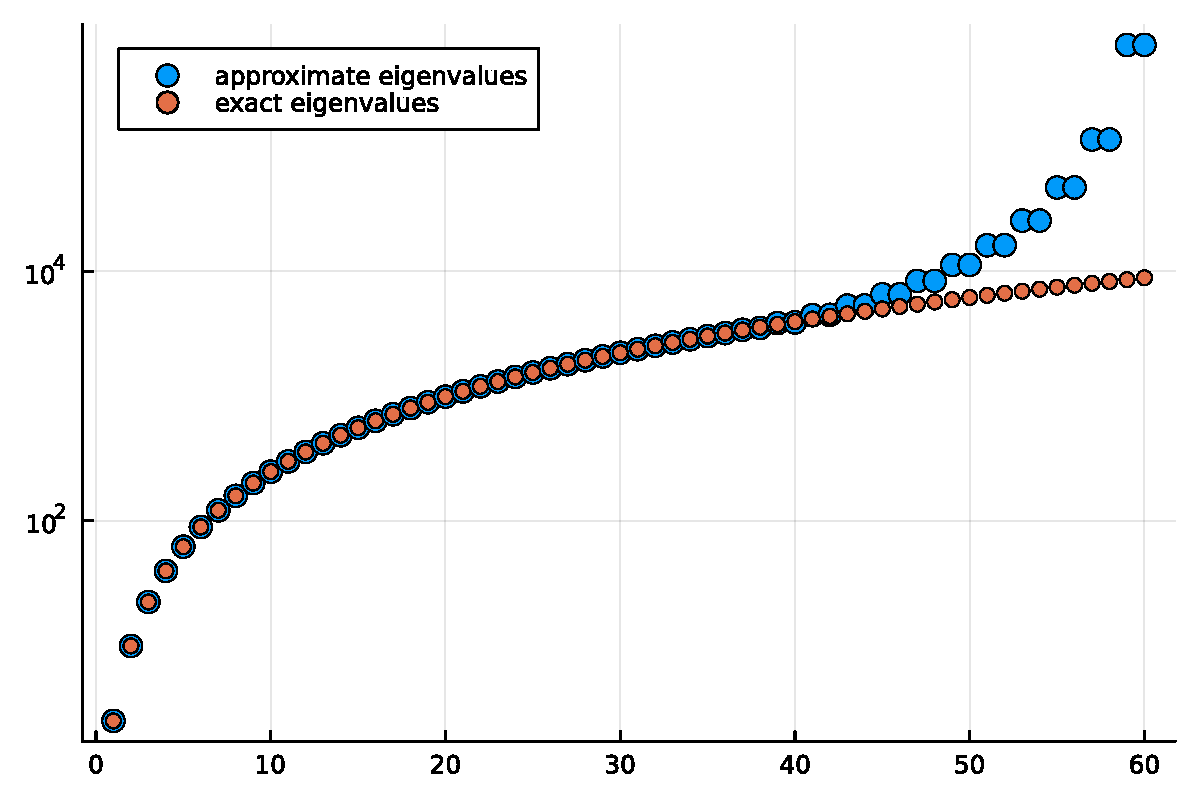
\includegraphics[width=\linewidth]{/figures/Chapter5_43_1.pdf}

Here are some of the eigenvectors of $A$:


\begin{lstlisting}
(*@\HLJLn{fact}@*) (*@\HLJLoB{=}@*) (*@\HLJLnf{eigen}@*)(*@\HLJLp{(}@*)(*@\HLJLn{A}@*)(*@\HLJLp{)}@*)
(*@\HLJLn{W}@*) (*@\HLJLoB{=}@*) (*@\HLJLn{fact}@*)(*@\HLJLoB{.}@*)(*@\HLJLn{vectors}@*)
(*@\HLJLn{p1}@*) (*@\HLJLoB{=}@*) (*@\HLJLnf{plot}@*)(*@\HLJLp{(}@*)(*@\HLJLn{s}@*)(*@\HLJLp{[}@*)(*@\HLJLni{2}@*)(*@\HLJLoB{:}@*)(*@\HLJLn{n}@*)(*@\HLJLp{],}@*)(*@\HLJLn{W}@*)(*@\HLJLp{[}@*)(*@\HLJLoB{:}@*)(*@\HLJLp{,}@*)(*@\HLJLn{n}@*)(*@\HLJLoB{-}@*)(*@\HLJLni{5}@*)(*@\HLJLp{];}@*)(*@\HLJLn{legend}@*)(*@\HLJLoB{=}@*)(*@\HLJLkc{false}@*)(*@\HLJLp{)}@*)
(*@\HLJLnf{scatter!}@*)(*@\HLJLp{(}@*)(*@\HLJLn{s}@*)(*@\HLJLp{[}@*)(*@\HLJLni{2}@*)(*@\HLJLoB{:}@*)(*@\HLJLn{n}@*)(*@\HLJLp{],}@*)(*@\HLJLn{W}@*)(*@\HLJLp{[}@*)(*@\HLJLoB{:}@*)(*@\HLJLp{,}@*)(*@\HLJLn{n}@*)(*@\HLJLoB{-}@*)(*@\HLJLni{5}@*)(*@\HLJLp{])}@*)
(*@\HLJLn{p2}@*) (*@\HLJLoB{=}@*) (*@\HLJLnf{plot}@*)(*@\HLJLp{(}@*)(*@\HLJLn{s}@*)(*@\HLJLp{[}@*)(*@\HLJLni{2}@*)(*@\HLJLoB{:}@*)(*@\HLJLn{n}@*)(*@\HLJLp{],}@*)(*@\HLJLn{W}@*)(*@\HLJLp{[}@*)(*@\HLJLoB{:}@*)(*@\HLJLp{,}@*)(*@\HLJLn{n}@*)(*@\HLJLoB{-}@*)(*@\HLJLni{10}@*)(*@\HLJLp{];}@*)(*@\HLJLn{legend}@*)(*@\HLJLoB{=}@*)(*@\HLJLkc{false}@*)(*@\HLJLp{)}@*)
(*@\HLJLnf{scatter!}@*)(*@\HLJLp{(}@*)(*@\HLJLn{s}@*)(*@\HLJLp{[}@*)(*@\HLJLni{2}@*)(*@\HLJLoB{:}@*)(*@\HLJLn{n}@*)(*@\HLJLp{],}@*)(*@\HLJLn{W}@*)(*@\HLJLp{[}@*)(*@\HLJLoB{:}@*)(*@\HLJLp{,}@*)(*@\HLJLn{n}@*)(*@\HLJLoB{-}@*)(*@\HLJLni{10}@*)(*@\HLJLp{])}@*)
(*@\HLJLn{p3}@*) (*@\HLJLoB{=}@*) (*@\HLJLnf{plot}@*)(*@\HLJLp{(}@*)(*@\HLJLn{s}@*)(*@\HLJLp{[}@*)(*@\HLJLni{2}@*)(*@\HLJLoB{:}@*)(*@\HLJLn{n}@*)(*@\HLJLp{],}@*)(*@\HLJLn{W}@*)(*@\HLJLp{[}@*)(*@\HLJLoB{:}@*)(*@\HLJLp{,}@*)(*@\HLJLni{20}@*)(*@\HLJLp{];}@*)(*@\HLJLn{legend}@*)(*@\HLJLoB{=}@*)(*@\HLJLkc{false}@*)(*@\HLJLp{)}@*)
(*@\HLJLnf{scatter!}@*)(*@\HLJLp{(}@*)(*@\HLJLn{s}@*)(*@\HLJLp{[}@*)(*@\HLJLni{2}@*)(*@\HLJLoB{:}@*)(*@\HLJLn{n}@*)(*@\HLJLp{],}@*)(*@\HLJLn{W}@*)(*@\HLJLp{[}@*)(*@\HLJLoB{:}@*)(*@\HLJLp{,}@*)(*@\HLJLni{20}@*)(*@\HLJLp{])}@*)
(*@\HLJLn{p4}@*) (*@\HLJLoB{=}@*) (*@\HLJLnf{plot}@*)(*@\HLJLp{(}@*)(*@\HLJLn{s}@*)(*@\HLJLp{[}@*)(*@\HLJLni{2}@*)(*@\HLJLoB{:}@*)(*@\HLJLn{n}@*)(*@\HLJLp{],}@*)(*@\HLJLn{W}@*)(*@\HLJLp{[}@*)(*@\HLJLoB{:}@*)(*@\HLJLp{,}@*)(*@\HLJLni{1}@*)(*@\HLJLp{];}@*)(*@\HLJLn{legend}@*)(*@\HLJLoB{=}@*)(*@\HLJLkc{false}@*)(*@\HLJLp{)}@*)
(*@\HLJLnf{scatter!}@*)(*@\HLJLp{(}@*)(*@\HLJLn{s}@*)(*@\HLJLp{[}@*)(*@\HLJLni{2}@*)(*@\HLJLoB{:}@*)(*@\HLJLn{n}@*)(*@\HLJLp{],}@*)(*@\HLJLn{W}@*)(*@\HLJLp{[}@*)(*@\HLJLoB{:}@*)(*@\HLJLp{,}@*)(*@\HLJLni{1}@*)(*@\HLJLp{])}@*)
(*@\HLJLnf{plot}@*)(*@\HLJLp{(}@*)(*@\HLJLn{p1}@*)(*@\HLJLp{,}@*)(*@\HLJLn{p2}@*)(*@\HLJLp{,}@*)(*@\HLJLn{p3}@*)(*@\HLJLp{,}@*)(*@\HLJLn{p4}@*)(*@\HLJLp{)}@*)
\end{lstlisting}

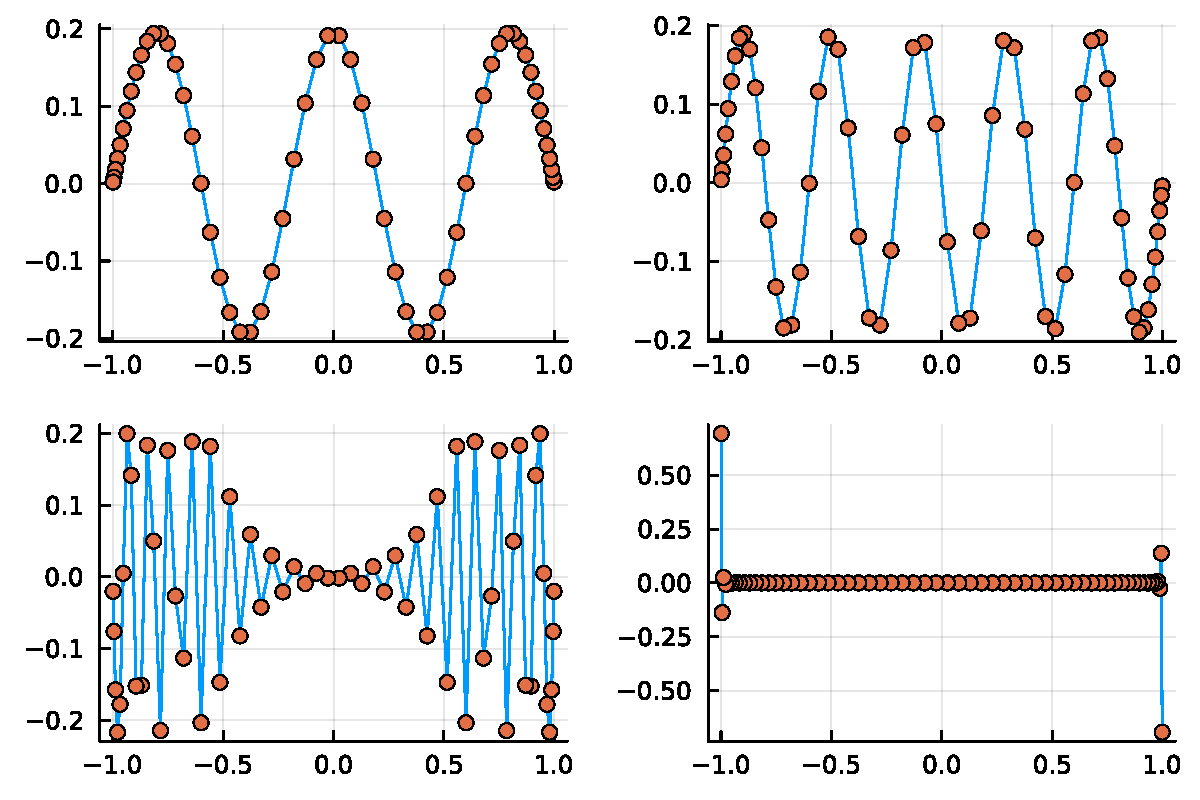
\includegraphics[width=\linewidth]{/figures/Chapter5_44_1.pdf}

Let's investigate how the spectral radius grows with $n$:


\begin{lstlisting}
(*@\HLJLn{nmax}@*) (*@\HLJLoB{=}@*) (*@\HLJLni{81}@*)(*@\HLJLp{;}@*) (*@\HLJLn{nvc}@*) (*@\HLJLoB{=}@*) (*@\HLJLni{5}@*)(*@\HLJLoB{:}@*)(*@\HLJLn{nmax}@*)
(*@\HLJLn{\ensuremath{\rho}c}@*) (*@\HLJLoB{=}@*) (*@\HLJLp{[(}@*) (*@\HLJLp{(}@*)(*@\HLJLn{D}@*)(*@\HLJLp{,}@*)(*@\HLJLoB{{\textasciitilde}}@*)(*@\HLJLp{)}@*) (*@\HLJLoB{=}@*) (*@\HLJLnf{cheb}@*)(*@\HLJLp{(}@*)(*@\HLJLn{n}@*)(*@\HLJLp{);}@*) (*@\HLJLn{D2}@*) (*@\HLJLoB{=}@*) (*@\HLJLn{D}@*)(*@\HLJLoB{{\textasciicircum}}@*)(*@\HLJLni{2}@*)(*@\HLJLp{;}@*) (*@\HLJLn{A}@*) (*@\HLJLoB{=}@*) (*@\HLJLn{D2}@*)(*@\HLJLp{[}@*)(*@\HLJLni{2}@*)(*@\HLJLoB{:}@*)(*@\HLJLn{n}@*)(*@\HLJLp{,}@*)(*@\HLJLni{2}@*)(*@\HLJLoB{:}@*)(*@\HLJLn{n}@*)(*@\HLJLp{];}@*) (*@\HLJLn{\ensuremath{\lambda}}@*) (*@\HLJLoB{=}@*) (*@\HLJLnf{eigvals}@*)(*@\HLJLp{(}@*)(*@\HLJLn{A}@*)(*@\HLJLp{);}@*)
    (*@\HLJLnf{norm}@*)(*@\HLJLp{(}@*)(*@\HLJLn{\ensuremath{\lambda}}@*)(*@\HLJLp{,}@*)(*@\HLJLn{Inf}@*)(*@\HLJLp{))}@*) (*@\HLJLk{for}@*) (*@\HLJLn{n}@*) (*@\HLJLoB{=}@*) (*@\HLJLn{nvc}@*)(*@\HLJLp{];}@*)
\end{lstlisting}


\begin{lstlisting}
(*@\HLJLnf{scatter}@*)(*@\HLJLp{(}@*)(*@\HLJLn{nvc}@*)(*@\HLJLoB{.-}@*)(*@\HLJLni{1}@*)(*@\HLJLp{,}@*)(*@\HLJLn{\ensuremath{\rho}c}@*)(*@\HLJLp{;}@*)(*@\HLJLn{yscale}@*)(*@\HLJLoB{=:}@*)(*@\HLJLn{log10}@*)(*@\HLJLp{,}@*)(*@\HLJLn{legend}@*)(*@\HLJLoB{=:}@*)(*@\HLJLn{topleft}@*)(*@\HLJLp{,}@*)(*@\HLJLn{label}@*)(*@\HLJLoB{=}@*)(*@\HLJLs{"{}spectral}@*) (*@\HLJLs{radius"{}}@*)(*@\HLJLp{)}@*)
(*@\HLJLnf{plot!}@*)(*@\HLJLp{(}@*)(*@\HLJLn{nvc}@*)(*@\HLJLoB{.-}@*)(*@\HLJLni{1}@*)(*@\HLJLp{,}@*)(*@\HLJLnfB{0.05}@*)(*@\HLJLoB{*}@*)(*@\HLJLp{(}@*)(*@\HLJLn{nvc}@*)(*@\HLJLoB{.-}@*)(*@\HLJLni{1}@*)(*@\HLJLp{)}@*)(*@\HLJLoB{.{\textasciicircum}}@*)(*@\HLJLni{4}@*)(*@\HLJLp{;}@*)(*@\HLJLn{label}@*)(*@\HLJLoB{=}@*)(*@\HLJLs{"{}0.05n\ensuremath{\^4}"{}}@*)(*@\HLJLp{)}@*)
\end{lstlisting}

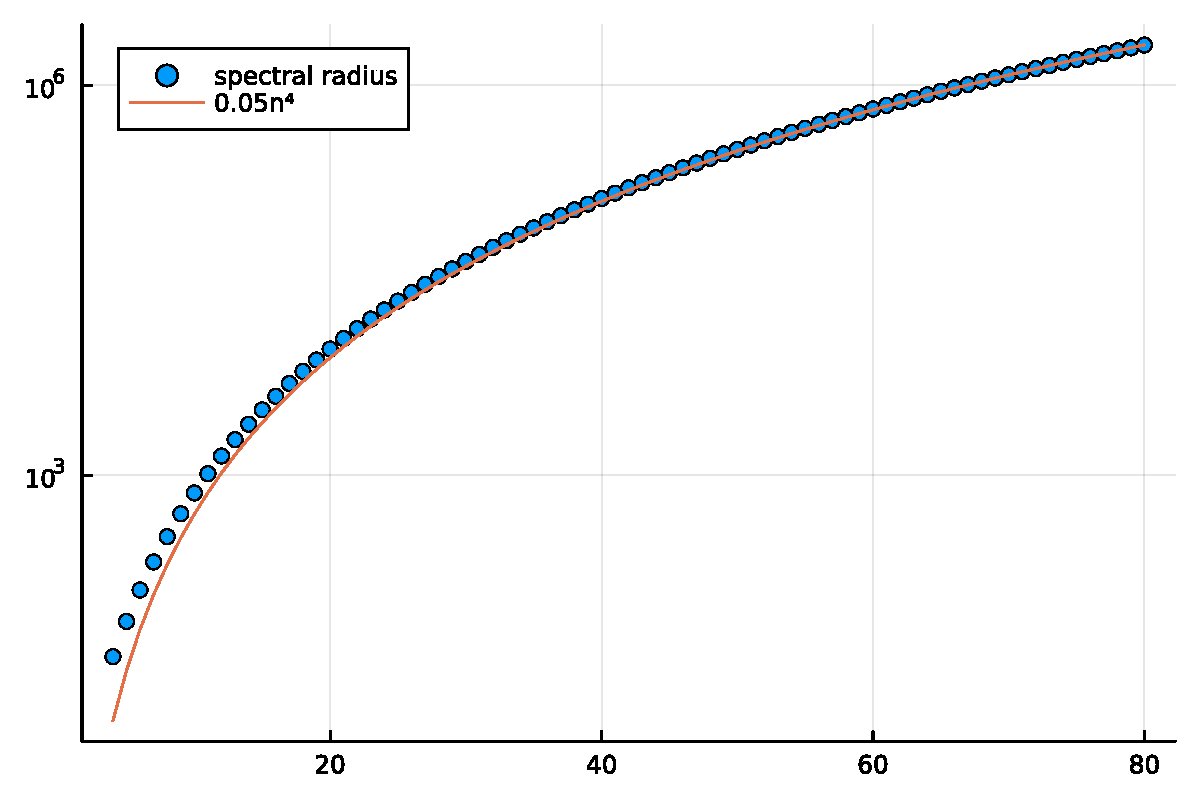
\includegraphics[width=\linewidth]{/figures/Chapter5_46_1.pdf}

Here's how the spectral condition number $\kappa(W)$ grows with $n$:


\begin{lstlisting}
(*@\HLJLn{nmax}@*) (*@\HLJLoB{=}@*) (*@\HLJLni{300}@*)
(*@\HLJLn{nv}@*) (*@\HLJLoB{=}@*) (*@\HLJLni{10}@*)(*@\HLJLoB{:}@*)(*@\HLJLni{10}@*)(*@\HLJLoB{:}@*)(*@\HLJLn{nmax}@*)
(*@\HLJLn{\ensuremath{\kappa}}@*) (*@\HLJLoB{=}@*) (*@\HLJLp{[(}@*) (*@\HLJLp{(}@*)(*@\HLJLn{D}@*)(*@\HLJLp{,}@*)(*@\HLJLoB{{\textasciitilde}}@*)(*@\HLJLp{)}@*) (*@\HLJLoB{=}@*) (*@\HLJLnf{cheb}@*)(*@\HLJLp{(}@*)(*@\HLJLn{n}@*)(*@\HLJLp{);}@*) (*@\HLJLn{D2}@*) (*@\HLJLoB{=}@*) (*@\HLJLn{D}@*)(*@\HLJLoB{{\textasciicircum}}@*)(*@\HLJLni{2}@*)(*@\HLJLp{;}@*) (*@\HLJLn{A}@*) (*@\HLJLoB{=}@*) (*@\HLJLn{D2}@*)(*@\HLJLp{[}@*)(*@\HLJLni{2}@*)(*@\HLJLoB{:}@*)(*@\HLJLn{n}@*)(*@\HLJLp{,}@*)(*@\HLJLni{2}@*)(*@\HLJLoB{:}@*)(*@\HLJLn{n}@*)(*@\HLJLp{];}@*) (*@\HLJLn{fact}@*) (*@\HLJLoB{=}@*) (*@\HLJLnf{eigen}@*)(*@\HLJLp{(}@*)(*@\HLJLn{A}@*)(*@\HLJLp{);}@*)
        (*@\HLJLnf{cond}@*)(*@\HLJLp{(}@*)(*@\HLJLn{fact}@*)(*@\HLJLoB{.}@*)(*@\HLJLn{vectors}@*)(*@\HLJLp{))}@*) (*@\HLJLk{for}@*) (*@\HLJLn{n}@*) (*@\HLJLoB{=}@*) (*@\HLJLn{nv}@*)(*@\HLJLp{];}@*)
\end{lstlisting}


\begin{lstlisting}
(*@\HLJLnf{scatter}@*)(*@\HLJLp{(}@*)(*@\HLJLn{nv}@*)(*@\HLJLp{,}@*)(*@\HLJLn{\ensuremath{\kappa}}@*)(*@\HLJLp{,}@*)(*@\HLJLn{label}@*)(*@\HLJLoB{=}@*)(*@\HLJLs{"{}spectral}@*) (*@\HLJLs{condition}@*) (*@\HLJLs{number"{}}@*)(*@\HLJLp{)}@*)
(*@\HLJLnf{plot!}@*)(*@\HLJLp{(}@*)(*@\HLJLn{nv}@*)(*@\HLJLp{,}@*)(*@\HLJLnfB{0.825}@*)(*@\HLJLoB{*}@*)(*@\HLJLn{nv}@*)(*@\HLJLoB{.{\textasciicircum}}@*)(*@\HLJLp{(}@*)(*@\HLJLni{1}@*)(*@\HLJLoB{/}@*)(*@\HLJLni{4}@*)(*@\HLJLp{);}@*)(*@\HLJLn{label}@*)(*@\HLJLoB{=}@*)(*@\HLJLs{"{}model"{}}@*)(*@\HLJLp{)}@*)
\end{lstlisting}

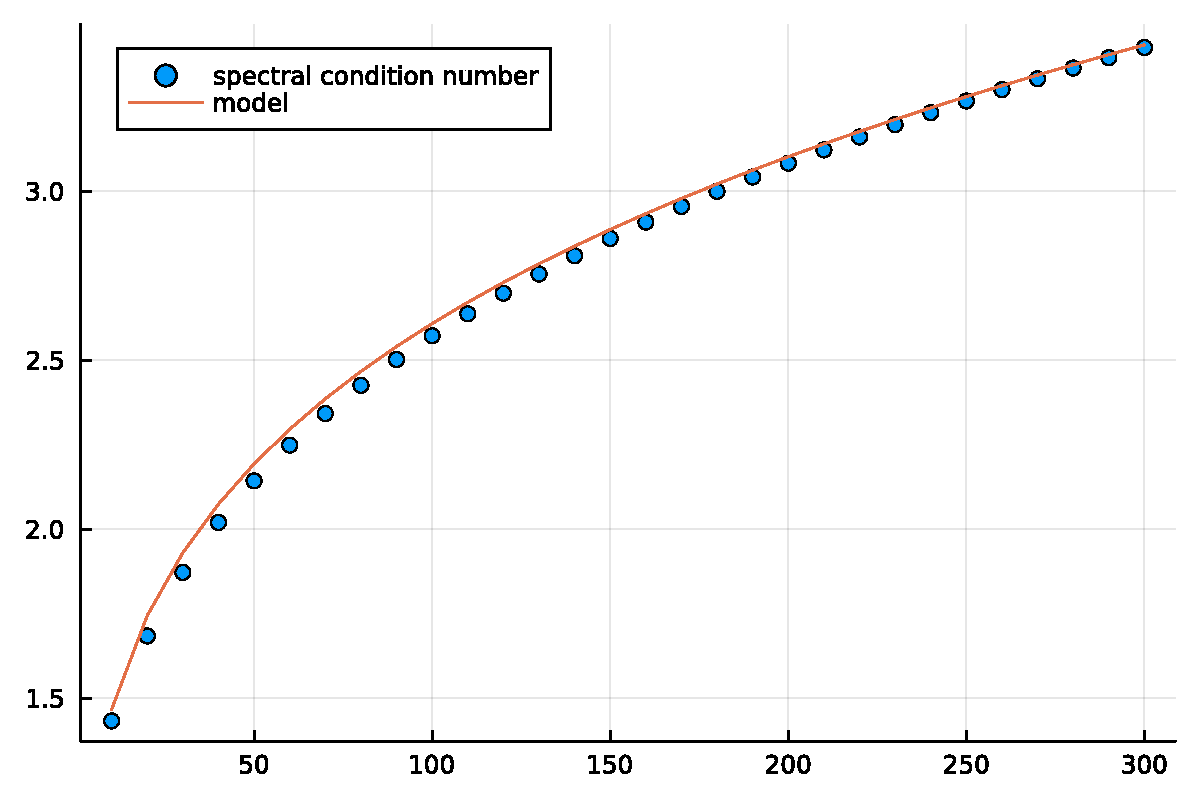
\includegraphics[width=\linewidth]{/figures/Chapter5_48_1.pdf}

Returning to the bound we derived above,

\[
\| {\rm e}^{tA} \| \leq \| W \| \| W^{-1} \| \| {\rm e}^{t\Lambda} \| = \kappa(W)\max\lbrace {\rm e}^{t\lambda} : \lambda \in \sigma(A)  \rbrace,
\]
from our numerical results we have the following estimate for an upper bound on $\| {\rm e}^{tA} \|$, namely,

\[
0.825 n^{1/4}{\rm e}^{-\pi^2 t/4}.
\]
It turns out this bound is completely too pessimistic:


\begin{lstlisting}
(*@\HLJLn{t}@*) (*@\HLJLoB{=}@*) (*@\HLJLnfB{0.1}@*)
(*@\HLJLn{nmax}@*) (*@\HLJLoB{=}@*) (*@\HLJLni{50}@*)
(*@\HLJLn{nv}@*) (*@\HLJLoB{=}@*) (*@\HLJLni{4}@*)(*@\HLJLoB{:}@*)(*@\HLJLn{nmax}@*)
(*@\HLJLn{mexpb}@*) (*@\HLJLoB{=}@*) (*@\HLJLp{[(}@*) (*@\HLJLp{(}@*)(*@\HLJLn{D}@*)(*@\HLJLp{,}@*)(*@\HLJLoB{{\textasciitilde}}@*)(*@\HLJLp{)}@*) (*@\HLJLoB{=}@*) (*@\HLJLnf{cheb}@*)(*@\HLJLp{(}@*)(*@\HLJLn{n}@*)(*@\HLJLp{);}@*) (*@\HLJLn{D2}@*) (*@\HLJLoB{=}@*) (*@\HLJLn{D}@*)(*@\HLJLoB{{\textasciicircum}}@*)(*@\HLJLni{2}@*)(*@\HLJLp{;}@*) (*@\HLJLn{A}@*) (*@\HLJLoB{=}@*) (*@\HLJLn{D2}@*)(*@\HLJLp{[}@*)(*@\HLJLni{2}@*)(*@\HLJLoB{:}@*)(*@\HLJLn{n}@*)(*@\HLJLp{,}@*)(*@\HLJLni{2}@*)(*@\HLJLoB{:}@*)(*@\HLJLn{n}@*)(*@\HLJLp{];}@*)
          (*@\HLJLnf{opnorm}@*)(*@\HLJLp{(}@*)(*@\HLJLnf{exp}@*)(*@\HLJLp{(}@*)(*@\HLJLn{t}@*)(*@\HLJLoB{*}@*)(*@\HLJLn{A}@*)(*@\HLJLp{),}@*)(*@\HLJLni{2}@*)(*@\HLJLp{))}@*)  (*@\HLJLk{for}@*) (*@\HLJLn{n}@*) (*@\HLJLoB{=}@*) (*@\HLJLn{nv}@*)(*@\HLJLp{]}@*)
(*@\HLJLnf{scatter}@*)(*@\HLJLp{(}@*)(*@\HLJLn{nv}@*)(*@\HLJLp{,}@*)(*@\HLJLn{mexpb}@*)(*@\HLJLp{;}@*)(*@\HLJLn{label}@*)(*@\HLJLoB{=}@*)(*@\HLJLs{"{}||}@*) (*@\HLJLs{exp(tA)}@*) (*@\HLJLs{||"{}}@*)(*@\HLJLp{)}@*)
(*@\HLJLnf{plot!}@*)(*@\HLJLp{(}@*)(*@\HLJLn{nv}@*)(*@\HLJLp{,}@*)(*@\HLJLnfB{0.825}@*)(*@\HLJLoB{*}@*)(*@\HLJLn{nv}@*)(*@\HLJLoB{.{\textasciicircum}}@*)(*@\HLJLp{(}@*)(*@\HLJLni{1}@*)(*@\HLJLoB{/}@*)(*@\HLJLni{4}@*)(*@\HLJLp{)}@*)(*@\HLJLoB{*}@*)(*@\HLJLnf{exp}@*)(*@\HLJLp{(}@*)(*@\HLJLoB{-}@*)(*@\HLJLn{\ensuremath{\pi}}@*)(*@\HLJLoB{{\textasciicircum}}@*)(*@\HLJLni{2}@*)(*@\HLJLoB{*}@*)(*@\HLJLn{t}@*)(*@\HLJLoB{/}@*)(*@\HLJLni{4}@*)(*@\HLJLp{);}@*)(*@\HLJLn{label}@*)(*@\HLJLoB{=}@*)(*@\HLJLs{"{}upper}@*) (*@\HLJLs{bound"{}}@*)(*@\HLJLp{)}@*)
\end{lstlisting}

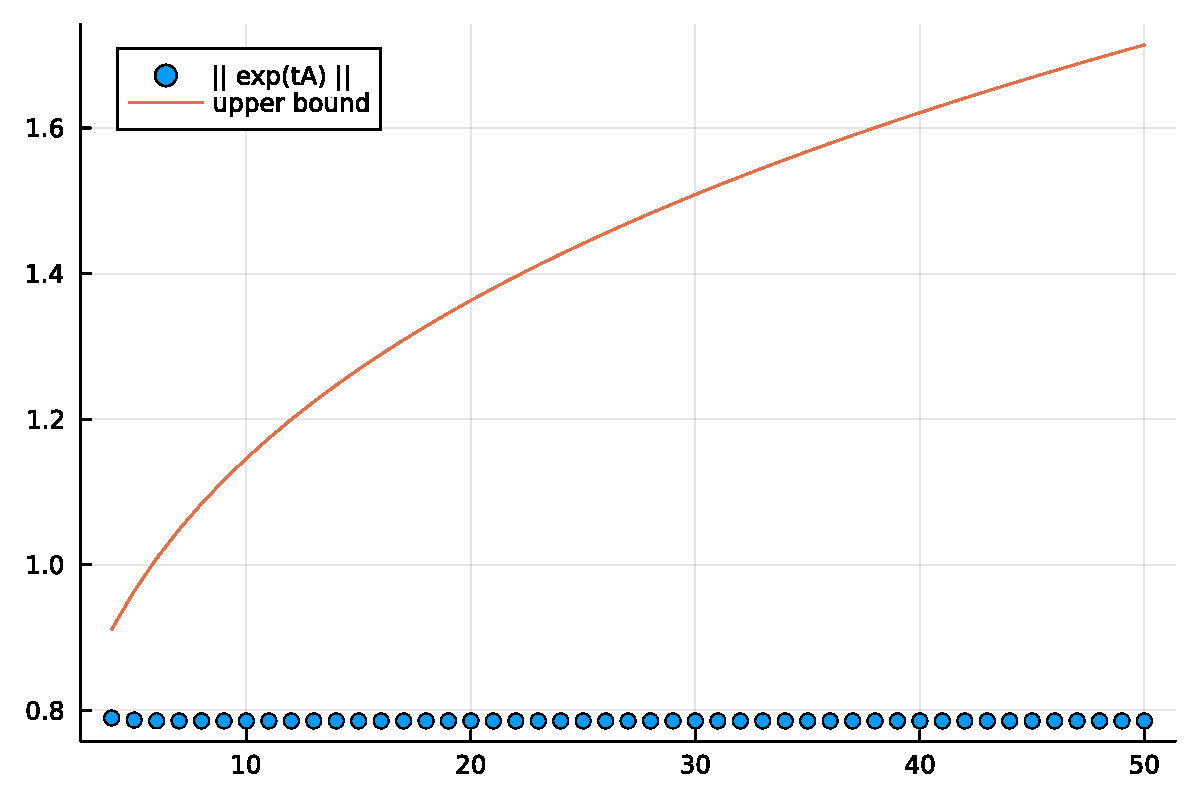
\includegraphics[width=\linewidth]{/figures/Chapter5_49_1.pdf}

Let's return to the linear ODE system we derived for the diffusion equation with the Chebyshev collocation method:

\[
\mathbf{v}'(t) = A\mathbf{v}(t) + \mathbf{h}(t), \qquad \mathbf{v}(t) \in \mathbb{R}^{n-1}, \qquad A \in \mathbb{R}^{(n-1)\times (n-1)}.
\]
Earlier in this chapter, we showed that if $A$ has an eigendecomposition, then this system can be diagonalised (i.e., the coupled system of ODEs can be expressed as $n-1$ decoupled scalar ODEs) and we derived the following step size restriction for Euler's method to be stable:

\[
\tau \leq \frac{2}{\rho(A)}.
\]
Based on our numerical results above, we estimate that

\[
\tau \leq \frac{2}{\rho(A)} \approx \frac{2}{4(0.05n^4)} = \frac{10}{n^4}.
\]
Let's test this:


\begin{lstlisting}
(*@\HLJLn{n}@*) (*@\HLJLoB{=}@*) (*@\HLJLni{24}@*)
(*@\HLJLn{f}@*) (*@\HLJLoB{=}@*) (*@\HLJLn{x}@*) (*@\HLJLoB{->}@*) (*@\HLJLnf{sin}@*)(*@\HLJLp{(}@*)(*@\HLJLn{\ensuremath{\pi}}@*)(*@\HLJLoB{*}@*)(*@\HLJLn{x}@*)(*@\HLJLoB{/}@*)(*@\HLJLni{2}@*)(*@\HLJLp{)}@*) (*@\HLJLoB{+}@*) (*@\HLJLnfB{0.5}@*)(*@\HLJLoB{*}@*)(*@\HLJLnf{sin}@*)(*@\HLJLp{(}@*)(*@\HLJLni{2}@*)(*@\HLJLn{\ensuremath{\pi}}@*)(*@\HLJLoB{*}@*)(*@\HLJLn{x}@*)(*@\HLJLp{)}@*)
(*@\HLJLn{\ensuremath{\phi}1}@*) (*@\HLJLoB{=}@*) (*@\HLJLn{t}@*) (*@\HLJLoB{->}@*) (*@\HLJLnf{exp}@*)(*@\HLJLp{(}@*)(*@\HLJLoB{-}@*)(*@\HLJLn{\ensuremath{\pi}}@*)(*@\HLJLoB{{\textasciicircum}}@*)(*@\HLJLni{2}@*)(*@\HLJLoB{*}@*)(*@\HLJLn{t}@*)(*@\HLJLoB{/}@*)(*@\HLJLni{4}@*)(*@\HLJLp{)}@*)
(*@\HLJLn{\ensuremath{\phi}0}@*) (*@\HLJLoB{=}@*) (*@\HLJLn{t}@*) (*@\HLJLoB{->}@*) (*@\HLJLni{0}@*)
(*@\HLJLn{T}@*) (*@\HLJLoB{=}@*) (*@\HLJLnfB{0.25}@*)
(*@\HLJLn{D}@*)(*@\HLJLp{,}@*)(*@\HLJLn{s}@*) (*@\HLJLoB{=}@*) (*@\HLJLnf{cheb}@*)(*@\HLJLp{(}@*)(*@\HLJLn{n}@*)(*@\HLJLp{)}@*)
(*@\HLJLn{x}@*) (*@\HLJLoB{=}@*) (*@\HLJLp{(}@*)(*@\HLJLn{s}@*) (*@\HLJLoB{.+}@*) (*@\HLJLni{1}@*)(*@\HLJLp{)}@*)(*@\HLJLoB{/}@*)(*@\HLJLni{2}@*)
(*@\HLJLn{D2}@*) (*@\HLJLoB{=}@*) (*@\HLJLn{D}@*)(*@\HLJLoB{{\textasciicircum}}@*)(*@\HLJLni{2}@*)
(*@\HLJLn{F}@*) (*@\HLJLoB{=}@*) (*@\HLJLp{(}@*)(*@\HLJLn{t}@*)(*@\HLJLp{,}@*)(*@\HLJLn{v}@*)(*@\HLJLp{)}@*) (*@\HLJLoB{->}@*) (*@\HLJLni{4}@*)(*@\HLJLn{D2}@*)(*@\HLJLp{[}@*)(*@\HLJLni{2}@*)(*@\HLJLoB{:}@*)(*@\HLJLn{n}@*)(*@\HLJLp{,}@*)(*@\HLJLni{2}@*)(*@\HLJLoB{:}@*)(*@\HLJLn{n}@*)(*@\HLJLp{]}@*)(*@\HLJLoB{*}@*)(*@\HLJLn{v}@*) (*@\HLJLoB{+}@*) (*@\HLJLni{4}@*)(*@\HLJLoB{*}@*)(*@\HLJLnf{\ensuremath{\phi}1}@*)(*@\HLJLp{(}@*)(*@\HLJLn{t}@*)(*@\HLJLp{)}@*)(*@\HLJLoB{*}@*)(*@\HLJLn{D2}@*)(*@\HLJLp{[}@*)(*@\HLJLni{2}@*)(*@\HLJLoB{:}@*)(*@\HLJLn{n}@*)(*@\HLJLp{,}@*)(*@\HLJLni{1}@*)(*@\HLJLp{]}@*) (*@\HLJLoB{+}@*) (*@\HLJLni{4}@*)(*@\HLJLoB{*}@*)(*@\HLJLnf{\ensuremath{\phi}0}@*)(*@\HLJLp{(}@*)(*@\HLJLn{t}@*)(*@\HLJLp{)}@*)(*@\HLJLoB{*}@*)(*@\HLJLn{D2}@*)(*@\HLJLp{[}@*)(*@\HLJLni{2}@*)(*@\HLJLoB{:}@*)(*@\HLJLn{n}@*)(*@\HLJLp{,}@*)(*@\HLJLn{n}@*)(*@\HLJLoB{+}@*)(*@\HLJLni{1}@*)(*@\HLJLp{]}@*)
(*@\HLJLn{\ensuremath{\tau}est}@*) (*@\HLJLoB{=}@*)  (*@\HLJLni{10}@*)(*@\HLJLoB{/}@*)(*@\HLJLn{n}@*)(*@\HLJLoB{{\textasciicircum}}@*)(*@\HLJLni{4}@*)
(*@\HLJLn{\ensuremath{\tau}}@*) (*@\HLJLoB{=}@*)  (*@\HLJLni{2}@*)(*@\HLJLoB{/}@*)(*@\HLJLp{(}@*)(*@\HLJLni{4}@*)(*@\HLJLoB{*}@*)(*@\HLJLnf{norm}@*)(*@\HLJLp{(}@*)(*@\HLJLnf{eigvals}@*)(*@\HLJLp{(}@*)(*@\HLJLn{D2}@*)(*@\HLJLp{[}@*)(*@\HLJLni{2}@*)(*@\HLJLoB{:}@*)(*@\HLJLn{n}@*)(*@\HLJLp{,}@*)(*@\HLJLni{2}@*)(*@\HLJLoB{:}@*)(*@\HLJLn{n}@*)(*@\HLJLp{]),}@*)(*@\HLJLn{Inf}@*)(*@\HLJLp{))}@*)
(*@\HLJLnd{@show}@*) (*@\HLJLp{[}@*)(*@\HLJLn{\ensuremath{\tau}}@*) (*@\HLJLn{\ensuremath{\tau}est}@*)(*@\HLJLp{]}@*)

(*@\HLJLcs{{\#}}@*) (*@\HLJLcs{Euler{\textquotesingle}s}@*) (*@\HLJLcs{method}@*)

(*@\HLJLn{t}@*) (*@\HLJLoB{=}@*) (*@\HLJLni{0}@*)(*@\HLJLoB{:}@*)(*@\HLJLn{\ensuremath{\tau}}@*)(*@\HLJLoB{:}@*)(*@\HLJLn{T}@*)
(*@\HLJLn{nt}@*) (*@\HLJLoB{=}@*) (*@\HLJLnf{length}@*)(*@\HLJLp{(}@*)(*@\HLJLn{t}@*)(*@\HLJLp{)}@*)(*@\HLJLoB{-}@*)(*@\HLJLni{1}@*)
(*@\HLJLnd{@show}@*) (*@\HLJLn{nt}@*)
(*@\HLJLn{u}@*) (*@\HLJLoB{=}@*) (*@\HLJLnf{zeros}@*)(*@\HLJLp{(}@*)(*@\HLJLn{n}@*)(*@\HLJLoB{-}@*)(*@\HLJLni{1}@*)(*@\HLJLp{,}@*)(*@\HLJLn{nt}@*)(*@\HLJLoB{+}@*)(*@\HLJLni{1}@*)(*@\HLJLp{);}@*) (*@\HLJLn{u}@*)(*@\HLJLp{[}@*)(*@\HLJLoB{:}@*)(*@\HLJLp{,}@*)(*@\HLJLni{1}@*)(*@\HLJLp{]}@*) (*@\HLJLoB{=}@*) (*@\HLJLn{f}@*)(*@\HLJLoB{.}@*)(*@\HLJLp{(}@*)(*@\HLJLn{x}@*)(*@\HLJLp{[}@*)(*@\HLJLni{2}@*)(*@\HLJLoB{:}@*)(*@\HLJLn{n}@*)(*@\HLJLp{])}@*)
(*@\HLJLnd{@time}@*) (*@\HLJLk{begin}@*)
(*@\HLJLk{for}@*) (*@\HLJLn{i}@*) (*@\HLJLoB{=}@*) (*@\HLJLni{1}@*)(*@\HLJLoB{:}@*)(*@\HLJLn{nt}@*)
    (*@\HLJLn{u}@*)(*@\HLJLp{[}@*)(*@\HLJLoB{:}@*)(*@\HLJLp{,}@*)(*@\HLJLn{i}@*)(*@\HLJLoB{+}@*)(*@\HLJLni{1}@*)(*@\HLJLp{]}@*) (*@\HLJLoB{=}@*) (*@\HLJLn{u}@*)(*@\HLJLp{[}@*)(*@\HLJLoB{:}@*)(*@\HLJLp{,}@*)(*@\HLJLn{i}@*)(*@\HLJLp{]}@*) (*@\HLJLoB{+}@*) (*@\HLJLn{\ensuremath{\tau}}@*)(*@\HLJLoB{*}@*)(*@\HLJLnf{F}@*)(*@\HLJLp{(}@*)(*@\HLJLn{t}@*)(*@\HLJLp{[}@*)(*@\HLJLn{i}@*)(*@\HLJLp{],}@*)(*@\HLJLn{u}@*)(*@\HLJLp{[}@*)(*@\HLJLoB{:}@*)(*@\HLJLp{,}@*)(*@\HLJLn{i}@*)(*@\HLJLp{])}@*)
(*@\HLJLk{end}@*)
(*@\HLJLk{end}@*)

(*@\HLJLnd{@gif}@*) (*@\HLJLk{for}@*) (*@\HLJLn{i}@*) (*@\HLJLoB{=}@*) (*@\HLJLni{1}@*)(*@\HLJLoB{:}@*)(*@\HLJLni{100}@*)(*@\HLJLoB{:}@*)(*@\HLJLn{nt}@*)(*@\HLJLoB{+}@*)(*@\HLJLni{1}@*)
    (*@\HLJLnf{plot}@*)(*@\HLJLp{(}@*)(*@\HLJLn{x}@*)(*@\HLJLp{[}@*)(*@\HLJLni{2}@*)(*@\HLJLoB{:}@*)(*@\HLJLn{n}@*)(*@\HLJLp{],}@*) (*@\HLJLn{u}@*)(*@\HLJLp{[}@*)(*@\HLJLoB{:}@*)(*@\HLJLp{,}@*)(*@\HLJLni{1}@*)(*@\HLJLp{],}@*) (*@\HLJLn{size}@*) (*@\HLJLoB{=}@*) (*@\HLJLp{(}@*)(*@\HLJLni{700}@*)(*@\HLJLp{,}@*) (*@\HLJLni{150}@*)(*@\HLJLp{),}@*) (*@\HLJLn{label}@*) (*@\HLJLoB{=}@*) (*@\HLJLs{"{}u0"{}}@*)(*@\HLJLp{)}@*)
    (*@\HLJLnf{plot!}@*)(*@\HLJLp{(}@*)(*@\HLJLn{x}@*)(*@\HLJLp{[}@*)(*@\HLJLni{2}@*)(*@\HLJLoB{:}@*)(*@\HLJLn{n}@*)(*@\HLJLp{],}@*) (*@\HLJLn{u}@*)(*@\HLJLp{[}@*)(*@\HLJLoB{:}@*)(*@\HLJLp{,}@*)(*@\HLJLn{i}@*)(*@\HLJLp{],}@*) (*@\HLJLn{lw}@*)(*@\HLJLoB{=}@*)(*@\HLJLni{2}@*)(*@\HLJLp{,}@*) (*@\HLJLn{label}@*) (*@\HLJLoB{=}@*) (*@\HLJLs{"{}Chebyshev}@*) (*@\HLJLs{collocation,t}@*) (*@\HLJLs{=}@*) (*@\HLJLs{"{}}@*) (*@\HLJLoB{*}@*) (*@\HLJLp{(}@*)(*@\HLJLnd{@sprintf}@*)(*@\HLJLp{(}@*)(*@\HLJLs{"{}{\%}.4f"{}}@*)(*@\HLJLp{,}@*) (*@\HLJLn{t}@*)(*@\HLJLp{[}@*)(*@\HLJLn{i}@*)(*@\HLJLp{])),}@*) (*@\HLJLn{legend}@*) (*@\HLJLoB{=}@*) (*@\HLJLsc{:outertopright}@*)(*@\HLJLp{)}@*)
    (*@\HLJLnf{plot!}@*)(*@\HLJLp{(}@*)(*@\HLJLn{xx}@*)(*@\HLJLp{,}@*) (*@\HLJLn{ue}@*)(*@\HLJLoB{.}@*)(*@\HLJLp{(}@*)(*@\HLJLn{xx}@*)(*@\HLJLp{,}@*)(*@\HLJLn{t}@*)(*@\HLJLp{[}@*)(*@\HLJLn{i}@*)(*@\HLJLp{]),}@*) (*@\HLJLn{label}@*) (*@\HLJLoB{=}@*) (*@\HLJLs{"{}exact}@*) (*@\HLJLs{solution"{}}@*)(*@\HLJLp{)}@*)
(*@\HLJLk{end}@*)
\end{lstlisting}

\begin{lstlisting}
[(*@\ensuremath{\tau}@*) (*@\ensuremath{\tau}@*)est] = [3.150641581125344e-5 3.0140817901234566e-5]
nt = 7934
  0.397192 seconds (482.43 k allocations: 108.321 MiB, 12.13(*@{{\%}}@*) gc time, 73.0
5(*@{{\%}}@*) compilation time)
Plots.AnimatedGif((*@{"{}}@*)C:(*@{{\textbackslash}}@*)(*@{{\textbackslash}}@*)Users(*@{{\textbackslash}}@*)(*@{{\textbackslash}}@*)mfaso(*@{{\textbackslash}}@*)(*@{{\textbackslash}}@*)AppData(*@{{\textbackslash}}@*)(*@{{\textbackslash}}@*)Local(*@{{\textbackslash}}@*)(*@{{\textbackslash}}@*)Temp(*@{{\textbackslash}}@*)(*@{{\textbackslash}}@*)jl(*@{{\_}}@*)Xt2YJwAqUz.gi
f(*@{"{}}@*))
\end{lstlisting}


\begin{lstlisting}
(*@\HLJLn{\ensuremath{\tau}}@*) (*@\HLJLoB{+=}@*) (*@\HLJLnfB{1E-7}@*)
(*@\HLJLn{t}@*) (*@\HLJLoB{=}@*) (*@\HLJLni{0}@*)(*@\HLJLoB{:}@*)(*@\HLJLn{\ensuremath{\tau}}@*)(*@\HLJLoB{:}@*)(*@\HLJLn{T}@*)(*@\HLJLp{;}@*) (*@\HLJLn{nt}@*) (*@\HLJLoB{=}@*) (*@\HLJLnf{length}@*)(*@\HLJLp{(}@*)(*@\HLJLn{t}@*)(*@\HLJLp{)}@*)(*@\HLJLoB{-}@*)(*@\HLJLni{1}@*)
(*@\HLJLnd{@show}@*) (*@\HLJLn{nt}@*)
(*@\HLJLn{u}@*) (*@\HLJLoB{=}@*) (*@\HLJLnf{zeros}@*)(*@\HLJLp{(}@*)(*@\HLJLn{n}@*)(*@\HLJLoB{-}@*)(*@\HLJLni{1}@*)(*@\HLJLp{,}@*)(*@\HLJLn{nt}@*)(*@\HLJLoB{+}@*)(*@\HLJLni{1}@*)(*@\HLJLp{);}@*) (*@\HLJLn{u}@*)(*@\HLJLp{[}@*)(*@\HLJLoB{:}@*)(*@\HLJLp{,}@*)(*@\HLJLni{1}@*)(*@\HLJLp{]}@*) (*@\HLJLoB{=}@*) (*@\HLJLn{f}@*)(*@\HLJLoB{.}@*)(*@\HLJLp{(}@*)(*@\HLJLn{x}@*)(*@\HLJLp{[}@*)(*@\HLJLni{2}@*)(*@\HLJLoB{:}@*)(*@\HLJLn{n}@*)(*@\HLJLp{])}@*)
(*@\HLJLnd{@time}@*) (*@\HLJLk{begin}@*)
(*@\HLJLk{for}@*) (*@\HLJLn{i}@*) (*@\HLJLoB{=}@*) (*@\HLJLni{1}@*)(*@\HLJLoB{:}@*)(*@\HLJLn{nt}@*)
    (*@\HLJLn{u}@*)(*@\HLJLp{[}@*)(*@\HLJLoB{:}@*)(*@\HLJLp{,}@*)(*@\HLJLn{i}@*)(*@\HLJLoB{+}@*)(*@\HLJLni{1}@*)(*@\HLJLp{]}@*) (*@\HLJLoB{=}@*) (*@\HLJLn{u}@*)(*@\HLJLp{[}@*)(*@\HLJLoB{:}@*)(*@\HLJLp{,}@*)(*@\HLJLn{i}@*)(*@\HLJLp{]}@*) (*@\HLJLoB{+}@*) (*@\HLJLn{\ensuremath{\tau}}@*)(*@\HLJLoB{*}@*)(*@\HLJLnf{F}@*)(*@\HLJLp{(}@*)(*@\HLJLn{t}@*)(*@\HLJLp{[}@*)(*@\HLJLn{i}@*)(*@\HLJLp{],}@*)(*@\HLJLn{u}@*)(*@\HLJLp{[}@*)(*@\HLJLoB{:}@*)(*@\HLJLp{,}@*)(*@\HLJLn{i}@*)(*@\HLJLp{])}@*)
(*@\HLJLk{end}@*)
(*@\HLJLk{end}@*)

(*@\HLJLnd{@gif}@*) (*@\HLJLk{for}@*) (*@\HLJLn{i}@*) (*@\HLJLoB{=}@*) (*@\HLJLni{1}@*)(*@\HLJLoB{:}@*)(*@\HLJLni{100}@*)(*@\HLJLoB{:}@*)(*@\HLJLn{nt}@*)(*@\HLJLoB{+}@*)(*@\HLJLni{1}@*)
    (*@\HLJLnf{plot}@*)(*@\HLJLp{(}@*)(*@\HLJLn{x}@*)(*@\HLJLp{[}@*)(*@\HLJLni{2}@*)(*@\HLJLoB{:}@*)(*@\HLJLn{n}@*)(*@\HLJLp{],}@*) (*@\HLJLn{u}@*)(*@\HLJLp{[}@*)(*@\HLJLoB{:}@*)(*@\HLJLp{,}@*)(*@\HLJLni{1}@*)(*@\HLJLp{],}@*) (*@\HLJLn{size}@*) (*@\HLJLoB{=}@*) (*@\HLJLp{(}@*)(*@\HLJLni{700}@*)(*@\HLJLp{,}@*) (*@\HLJLni{150}@*)(*@\HLJLp{),}@*) (*@\HLJLn{label}@*) (*@\HLJLoB{=}@*) (*@\HLJLs{"{}u0"{}}@*)(*@\HLJLp{)}@*)
    (*@\HLJLnf{plot!}@*)(*@\HLJLp{(}@*)(*@\HLJLn{x}@*)(*@\HLJLp{[}@*)(*@\HLJLni{2}@*)(*@\HLJLoB{:}@*)(*@\HLJLn{n}@*)(*@\HLJLp{],}@*) (*@\HLJLn{u}@*)(*@\HLJLp{[}@*)(*@\HLJLoB{:}@*)(*@\HLJLp{,}@*)(*@\HLJLn{i}@*)(*@\HLJLp{],}@*) (*@\HLJLn{lw}@*)(*@\HLJLoB{=}@*)(*@\HLJLni{2}@*)(*@\HLJLp{,}@*) (*@\HLJLn{label}@*) (*@\HLJLoB{=}@*) (*@\HLJLs{"{}Chebyshev}@*) (*@\HLJLs{collocation,t}@*) (*@\HLJLs{=}@*) (*@\HLJLs{"{}}@*) (*@\HLJLoB{*}@*) (*@\HLJLp{(}@*)(*@\HLJLnd{@sprintf}@*)(*@\HLJLp{(}@*)(*@\HLJLs{"{}{\%}.4f"{}}@*)(*@\HLJLp{,}@*) (*@\HLJLn{t}@*)(*@\HLJLp{[}@*)(*@\HLJLn{i}@*)(*@\HLJLp{])),}@*) (*@\HLJLn{legend}@*) (*@\HLJLoB{=}@*) (*@\HLJLsc{:outertopright}@*)(*@\HLJLp{)}@*)
    (*@\HLJLnf{plot!}@*)(*@\HLJLp{(}@*)(*@\HLJLn{xx}@*)(*@\HLJLp{,}@*) (*@\HLJLn{ue}@*)(*@\HLJLoB{.}@*)(*@\HLJLp{(}@*)(*@\HLJLn{xx}@*)(*@\HLJLp{,}@*)(*@\HLJLn{t}@*)(*@\HLJLp{[}@*)(*@\HLJLn{i}@*)(*@\HLJLp{]),}@*) (*@\HLJLn{label}@*) (*@\HLJLoB{=}@*) (*@\HLJLs{"{}exact}@*) (*@\HLJLs{solution"{}}@*)(*@\HLJLp{)}@*)
(*@\HLJLk{end}@*)
\end{lstlisting}

\begin{lstlisting}
nt = 7909
  0.161710 seconds (234.21 k allocations: 87.448 MiB, 29.44(*@{{\%}}@*) gc time)
Plots.AnimatedGif((*@{"{}}@*)C:(*@{{\textbackslash}}@*)(*@{{\textbackslash}}@*)Users(*@{{\textbackslash}}@*)(*@{{\textbackslash}}@*)mfaso(*@{{\textbackslash}}@*)(*@{{\textbackslash}}@*)AppData(*@{{\textbackslash}}@*)(*@{{\textbackslash}}@*)Local(*@{{\textbackslash}}@*)(*@{{\textbackslash}}@*)Temp(*@{{\textbackslash}}@*)(*@{{\textbackslash}}@*)jl(*@{{\_}}@*)QzcJVJA0Gv.gi
f(*@{"{}}@*))
\end{lstlisting}


Notice that the (spurious) exponentially growing solution produced by Euler's method appears to resemble the high-frequency eigenfunctions we plotted before.

Of course, there are much better time stepping methods than Euler's method:


\begin{lstlisting}
(*@\HLJLn{F}@*) (*@\HLJLoB{=}@*) (*@\HLJLp{(}@*)(*@\HLJLn{v}@*)(*@\HLJLp{,}@*)(*@\HLJLn{p}@*)(*@\HLJLp{,}@*)(*@\HLJLn{t}@*)(*@\HLJLp{)}@*) (*@\HLJLoB{->}@*) (*@\HLJLni{4}@*)(*@\HLJLn{D2}@*)(*@\HLJLp{[}@*)(*@\HLJLni{2}@*)(*@\HLJLoB{:}@*)(*@\HLJLn{n}@*)(*@\HLJLp{,}@*)(*@\HLJLni{2}@*)(*@\HLJLoB{:}@*)(*@\HLJLn{n}@*)(*@\HLJLp{]}@*)(*@\HLJLoB{*}@*)(*@\HLJLn{v}@*) (*@\HLJLoB{+}@*) (*@\HLJLni{4}@*)(*@\HLJLoB{*}@*)(*@\HLJLnf{\ensuremath{\phi}1}@*)(*@\HLJLp{(}@*)(*@\HLJLn{t}@*)(*@\HLJLp{)}@*)(*@\HLJLoB{*}@*)(*@\HLJLn{D2}@*)(*@\HLJLp{[}@*)(*@\HLJLni{2}@*)(*@\HLJLoB{:}@*)(*@\HLJLn{n}@*)(*@\HLJLp{,}@*)(*@\HLJLni{1}@*)(*@\HLJLp{]}@*) (*@\HLJLoB{+}@*) (*@\HLJLni{4}@*)(*@\HLJLoB{*}@*)(*@\HLJLnf{\ensuremath{\phi}0}@*)(*@\HLJLp{(}@*)(*@\HLJLn{t}@*)(*@\HLJLp{)}@*)(*@\HLJLoB{*}@*)(*@\HLJLn{D2}@*)(*@\HLJLp{[}@*)(*@\HLJLni{2}@*)(*@\HLJLoB{:}@*)(*@\HLJLn{n}@*)(*@\HLJLp{,}@*)(*@\HLJLn{n}@*)(*@\HLJLoB{+}@*)(*@\HLJLni{1}@*)(*@\HLJLp{]}@*)
(*@\HLJLn{prob}@*) (*@\HLJLoB{=}@*) (*@\HLJLnf{ODEProblem}@*)(*@\HLJLp{(}@*)(*@\HLJLn{F}@*)(*@\HLJLp{,}@*) (*@\HLJLn{f}@*)(*@\HLJLoB{.}@*)(*@\HLJLp{(}@*)(*@\HLJLn{x}@*)(*@\HLJLp{[}@*)(*@\HLJLni{2}@*)(*@\HLJLoB{:}@*)(*@\HLJLn{n}@*)(*@\HLJLp{]),}@*) (*@\HLJLp{(}@*)(*@\HLJLnfB{0.0}@*)(*@\HLJLp{,}@*) (*@\HLJLn{T}@*)(*@\HLJLp{))}@*)
(*@\HLJLn{soln}@*) (*@\HLJLoB{=}@*)  (*@\HLJLnf{solve}@*)(*@\HLJLp{(}@*)(*@\HLJLn{prob}@*)(*@\HLJLp{,}@*)(*@\HLJLnf{Rodas4}@*)(*@\HLJLp{(),}@*)(*@\HLJLn{abstol}@*)(*@\HLJLoB{=}@*)(*@\HLJLnfB{1e-4}@*)(*@\HLJLp{);}@*)
(*@\HLJLnf{length}@*)(*@\HLJLp{(}@*)(*@\HLJLn{soln}@*)(*@\HLJLoB{.}@*)(*@\HLJLn{t}@*)(*@\HLJLp{)}@*)
\end{lstlisting}

\begin{lstlisting}
13
\end{lstlisting}


\subsubsection{Chebyshev / ultraspherical spectral method}
Here we use the orthogonal polynomials we learnt about in Chapter 4 to approximate the solution to the diffusion equation in coefficient space.  Specifically, we assume the solution has an expansion in Chebyshev polynomials with time-dependent expansion coefficients, i.e., we assume

\[
u(x,t) = \sum_{k = 0}^{\infty}u_k(t)T_k(2x-1), \qquad x \in [0, 1], \qquad t \in [0, T].
\]
Setting

\[
T(2x-1) = \left[T_0(2x-1) | T_1(2x-1) | \cdots \right]
\]
and

\[
\mathbf{u}(t) = \left(
\begin{array}{c}
u_0(t) \\
u_1(t) \\
\vdots
\end{array}
\right)
\]
we can write

\[
u(x,t) = T(2x-1)\mathbf{u}(t).
\]
Recall from Chapter 4 that

\[
\frac{{\rm d}}{{\rm d}s} T(s) = C^{(1)}(s)\mathcal{D}_0, \qquad s \in [-1, 1],
\]
where

\[
C^{(1)}(s) = \left[C_0^{(1)}(s) | C_1^{(1)}(s) | \cdots \right]
\]
and $\mathcal{D}_0$ is a banded matrix with bandwidths $(-1, 1)$.  Also,

\[
\frac{{\rm d}^2}{{\rm d}s^2} T(s) = \frac{{\rm d}}{{\rm d}s}C^{(1)}(s)\mathcal{D}_0 = C^{(2)}(s)\mathcal{D}_1\mathcal{D}_0
\]
where $\mathcal{D}_1$ is an infinite matrix with bandwidths $(-1, 1)$ and therefore, setting $s = 2x -1$, we have

\[
\frac{\partial^2}{\partial x^2} u(x,t) = \frac{{\rm d}^2}{{\rm d}x^2} T(2x-1)\mathbf{u}(t) = 4C^{(2)}(2x-1)\mathcal{D}_1\mathcal{D}_0 \mathbf{u}(t).
\]
We therefore need to express the time derivative in the $C^{(2)}$ basis:

\[
\frac{\partial}{\partial t} u(x,t) = T(2x-1)\mathbf{u}'(t) = C^{(1)}(2x-1)\mathcal{S}_0\mathbf{u}'(t)  = C^{(2)}(2x-1)\mathcal{S}_1\mathcal{S}_0\mathbf{u}'(t),
\]
where $\mathcal{S}_0$ and $\mathcal{S}_1$ are infinite banded matrices with bandwidths $(0, 2)$ (see chapter 4).  Setting $u_t=u_{xx}$, we conclude that

\[
\mathcal{S}_1\mathcal{S}_0\mathbf{u}'(t) = 4\mathcal{D}_1\mathcal{D}_0 \mathbf{u}(t)
\]
From the initial data, we require

\[
u(x,0) = T(2x-1)\mathbf{u}(0) = \sum_{k=0}^{\infty}T_k(2x-1)u_k(0) = f(x).
\]
As we know from Chapter 3, we can approximate the Chebyshev coefficients $u_k(0)$ of $f(x)$ using the FFT or, in Julia we can use ApproxFun.jl, in Matlab we can use Chebfun and in Python, ChebyPy.


\begin{lstlisting}
(*@\HLJLn{f}@*) (*@\HLJLoB{=}@*) (*@\HLJLn{x}@*) (*@\HLJLoB{->}@*) (*@\HLJLnf{sin}@*)(*@\HLJLp{(}@*)(*@\HLJLn{\ensuremath{\pi}}@*)(*@\HLJLoB{*}@*)(*@\HLJLn{x}@*)(*@\HLJLoB{/}@*)(*@\HLJLni{2}@*)(*@\HLJLp{)}@*) (*@\HLJLoB{+}@*) (*@\HLJLnfB{0.5}@*)(*@\HLJLoB{*}@*)(*@\HLJLnf{sin}@*)(*@\HLJLp{(}@*)(*@\HLJLni{2}@*)(*@\HLJLn{\ensuremath{\pi}}@*)(*@\HLJLoB{*}@*)(*@\HLJLn{x}@*)(*@\HLJLp{)}@*)
(*@\HLJLn{fs}@*) (*@\HLJLoB{=}@*) (*@\HLJLn{s}@*) (*@\HLJLoB{->}@*) (*@\HLJLnf{f}@*)(*@\HLJLp{((}@*)(*@\HLJLn{s}@*)(*@\HLJLoB{+}@*)(*@\HLJLni{1}@*)(*@\HLJLp{)}@*)(*@\HLJLoB{/}@*)(*@\HLJLni{2}@*)(*@\HLJLp{)}@*)
(*@\HLJLn{g}@*) (*@\HLJLoB{=}@*) (*@\HLJLn{\ensuremath{\theta}}@*) (*@\HLJLoB{->}@*) (*@\HLJLnf{fs}@*)(*@\HLJLp{(}@*)(*@\HLJLnf{cos}@*)(*@\HLJLp{(}@*)(*@\HLJLn{\ensuremath{\theta}}@*)(*@\HLJLp{))}@*)
(*@\HLJLn{n}@*) (*@\HLJLoB{=}@*) (*@\HLJLni{30}@*)
(*@\HLJLn{\ensuremath{\theta}}@*) (*@\HLJLoB{=}@*) (*@\HLJLnf{range}@*)(*@\HLJLp{(}@*)(*@\HLJLni{0}@*)(*@\HLJLp{,}@*)(*@\HLJLni{2}@*)(*@\HLJLn{\ensuremath{\pi}}@*)(*@\HLJLp{;}@*)(*@\HLJLn{length}@*)(*@\HLJLoB{=}@*) (*@\HLJLni{2}@*)(*@\HLJLn{n}@*)(*@\HLJLoB{+}@*)(*@\HLJLni{2}@*)(*@\HLJLp{)[}@*)(*@\HLJLni{1}@*)(*@\HLJLoB{:}@*)(*@\HLJLk{end}@*)(*@\HLJLoB{-}@*)(*@\HLJLni{1}@*)(*@\HLJLp{]}@*) (*@\HLJLcs{{\#}}@*) (*@\HLJLcs{the}@*) (*@\HLJLcs{points}@*) (*@\HLJLcs{\ensuremath{\theta}{\_}j}@*)
(*@\HLJLn{ct}@*) (*@\HLJLoB{=}@*) (*@\HLJLnf{fft}@*)(*@\HLJLp{(}@*)(*@\HLJLn{g}@*)(*@\HLJLoB{.}@*)(*@\HLJLp{(}@*)(*@\HLJLn{\ensuremath{\theta}}@*)(*@\HLJLp{))}@*)(*@\HLJLoB{/}@*)(*@\HLJLp{(}@*)(*@\HLJLni{2}@*)(*@\HLJLn{n}@*)(*@\HLJLoB{+}@*)(*@\HLJLni{1}@*)(*@\HLJLp{)}@*) (*@\HLJLcs{{\#}}@*) (*@\HLJLcs{compute}@*) (*@\HLJLcs{approximate}@*) (*@\HLJLcs{Fourier}@*) (*@\HLJLcs{coefficients}@*) (*@\HLJLcs{of}@*) (*@\HLJLcs{g}@*)
(*@\HLJLcs{{\#}}@*) (*@\HLJLcs{approximate}@*) (*@\HLJLcs{Chebyshev}@*) (*@\HLJLcs{coefficients}@*)
(*@\HLJLn{ut}@*) (*@\HLJLoB{=}@*) (*@\HLJLp{[}@*)(*@\HLJLn{ct}@*)(*@\HLJLp{[}@*)(*@\HLJLni{1}@*)(*@\HLJLp{];}@*)(*@\HLJLni{2}@*)(*@\HLJLn{ct}@*)(*@\HLJLp{[}@*)(*@\HLJLni{2}@*)(*@\HLJLoB{:}@*)(*@\HLJLn{n}@*)(*@\HLJLoB{+}@*)(*@\HLJLni{1}@*)(*@\HLJLp{]]}@*) 
(*@\HLJLn{fc}@*) (*@\HLJLoB{=}@*) (*@\HLJLnf{Fun}@*)(*@\HLJLp{(}@*)(*@\HLJLn{f}@*)(*@\HLJLp{,}@*)(*@\HLJLnf{Chebyshev}@*)(*@\HLJLp{(}@*)(*@\HLJLnfB{0..1}@*)(*@\HLJLp{))}@*)
(*@\HLJLn{n}@*) (*@\HLJLoB{=}@*) (*@\HLJLnd{@show}@*) (*@\HLJLnf{length}@*)(*@\HLJLp{(}@*)(*@\HLJLn{fc}@*)(*@\HLJLoB{.}@*)(*@\HLJLn{coefficients}@*)(*@\HLJLp{)}@*)
(*@\HLJLnf{norm}@*)(*@\HLJLp{(}@*)(*@\HLJLn{fc}@*)(*@\HLJLoB{.}@*)(*@\HLJLn{coefficients}@*) (*@\HLJLoB{-}@*) (*@\HLJLn{ut}@*)(*@\HLJLp{[}@*)(*@\HLJLni{1}@*)(*@\HLJLoB{:}@*)(*@\HLJLn{n}@*)(*@\HLJLp{],}@*)(*@\HLJLn{Inf}@*)(*@\HLJLp{)}@*)
\end{lstlisting}

\begin{lstlisting}
length(fc.coefficients) = 22
1.5484256077849816e-16
\end{lstlisting}


Let's compute the solution to the system of ODEs

\[
\mathcal{S}_1\mathcal{S}_0\mathbf{u}'(t) = 4\mathcal{D}_1\mathcal{D}_0 \mathbf{u}(t),
\]
where we truncate the infinite system and $\mathbf{u}(0)$ is replaced with a finite vector of approximate Chebyshev coefficients of $f(x)$. 


\begin{lstlisting}
(*@\HLJLn{S10}@*) (*@\HLJLoB{=}@*) (*@\HLJLnf{Conversion}@*)(*@\HLJLp{(}@*)(*@\HLJLnf{Chebyshev}@*)(*@\HLJLp{(),}@*)(*@\HLJLnf{Ultraspherical}@*)(*@\HLJLp{(}@*)(*@\HLJLni{2}@*)(*@\HLJLp{))}@*)
(*@\HLJLn{D10}@*) (*@\HLJLoB{=}@*) (*@\HLJLnf{Derivative}@*)(*@\HLJLp{(}@*)(*@\HLJLnf{Chebyshev}@*)(*@\HLJLp{(),}@*)(*@\HLJLni{2}@*)(*@\HLJLp{)}@*)
(*@\HLJLn{L}@*) (*@\HLJLoB{=}@*) (*@\HLJLn{S10}@*)(*@\HLJLp{[}@*)(*@\HLJLni{1}@*)(*@\HLJLoB{:}@*)(*@\HLJLn{n}@*)(*@\HLJLp{,}@*)(*@\HLJLni{1}@*)(*@\HLJLoB{:}@*)(*@\HLJLn{n}@*)(*@\HLJLp{]}@*)
(*@\HLJLn{R}@*) (*@\HLJLoB{=}@*) (*@\HLJLni{4}@*)(*@\HLJLoB{*}@*)(*@\HLJLn{D10}@*)(*@\HLJLp{[}@*)(*@\HLJLni{1}@*)(*@\HLJLoB{:}@*)(*@\HLJLn{n}@*)(*@\HLJLp{,}@*)(*@\HLJLni{1}@*)(*@\HLJLoB{:}@*)(*@\HLJLn{n}@*)(*@\HLJLp{]}@*)
(*@\HLJLn{T}@*) (*@\HLJLoB{=}@*) (*@\HLJLnfB{0.1}@*)
(*@\HLJLn{F}@*) (*@\HLJLoB{=}@*) (*@\HLJLp{(}@*)(*@\HLJLn{u}@*)(*@\HLJLp{,}@*)(*@\HLJLn{p}@*)(*@\HLJLp{,}@*)(*@\HLJLn{t}@*)(*@\HLJLp{)}@*) (*@\HLJLoB{->}@*) (*@\HLJLn{L}@*)(*@\HLJLoB{{\textbackslash}}@*)(*@\HLJLp{(}@*)(*@\HLJLn{R}@*)(*@\HLJLoB{*}@*)(*@\HLJLn{u}@*)(*@\HLJLp{)}@*)
(*@\HLJLn{prob}@*) (*@\HLJLoB{=}@*) (*@\HLJLnf{ODEProblem}@*)(*@\HLJLp{(}@*)(*@\HLJLn{F}@*)(*@\HLJLp{,}@*) (*@\HLJLn{fc}@*)(*@\HLJLoB{.}@*)(*@\HLJLn{coefficients}@*)(*@\HLJLp{,}@*) (*@\HLJLp{(}@*)(*@\HLJLnfB{0.0}@*)(*@\HLJLp{,}@*) (*@\HLJLn{T}@*)(*@\HLJLp{))}@*)
(*@\HLJLn{soln}@*) (*@\HLJLoB{=}@*)  (*@\HLJLnf{solve}@*)(*@\HLJLp{(}@*)(*@\HLJLn{prob}@*)(*@\HLJLp{,}@*)(*@\HLJLnf{RK4}@*)(*@\HLJLp{(),}@*)(*@\HLJLn{reltol}@*)(*@\HLJLoB{=}@*)(*@\HLJLnfB{1E-6}@*)(*@\HLJLp{);}@*)
\end{lstlisting}


\begin{lstlisting}
(*@\HLJLn{xx}@*) (*@\HLJLoB{=}@*) (*@\HLJLnf{range}@*)(*@\HLJLp{(}@*)(*@\HLJLni{0}@*)(*@\HLJLp{,}@*)(*@\HLJLni{1}@*)(*@\HLJLp{;}@*)(*@\HLJLn{length}@*)(*@\HLJLoB{=}@*)(*@\HLJLni{301}@*)(*@\HLJLp{)}@*)
(*@\HLJLn{t}@*) (*@\HLJLoB{=}@*) (*@\HLJLn{soln}@*)(*@\HLJLoB{.}@*)(*@\HLJLn{t}@*)
(*@\HLJLn{u}@*) (*@\HLJLoB{=}@*) (*@\HLJLn{soln}@*)(*@\HLJLoB{.}@*)(*@\HLJLn{u}@*)
(*@\HLJLn{S}@*) (*@\HLJLoB{=}@*) (*@\HLJLnf{Chebyshev}@*)(*@\HLJLp{(}@*)(*@\HLJLnfB{0..1}@*)(*@\HLJLp{)}@*)
(*@\HLJLn{nt}@*) (*@\HLJLoB{=}@*) (*@\HLJLnf{length}@*)(*@\HLJLp{(}@*)(*@\HLJLn{soln}@*)(*@\HLJLoB{.}@*)(*@\HLJLn{t}@*)(*@\HLJLp{)}@*)
(*@\HLJLnd{@gif}@*) (*@\HLJLk{for}@*) (*@\HLJLn{i}@*) (*@\HLJLoB{=}@*) (*@\HLJLni{1}@*)(*@\HLJLoB{:}@*)(*@\HLJLn{nt}@*)
    (*@\HLJLnf{plot}@*)(*@\HLJLp{(}@*)(*@\HLJLn{xx}@*)(*@\HLJLp{,}@*) (*@\HLJLnf{Fun}@*)(*@\HLJLp{(}@*)(*@\HLJLn{S}@*)(*@\HLJLp{,}@*)(*@\HLJLn{u}@*)(*@\HLJLp{[}@*)(*@\HLJLni{1}@*)(*@\HLJLp{])}@*)(*@\HLJLoB{.}@*)(*@\HLJLp{(}@*)(*@\HLJLn{xx}@*)(*@\HLJLp{),}@*) (*@\HLJLn{size}@*) (*@\HLJLoB{=}@*) (*@\HLJLp{(}@*)(*@\HLJLni{700}@*)(*@\HLJLp{,}@*) (*@\HLJLni{150}@*)(*@\HLJLp{),}@*) (*@\HLJLn{label}@*) (*@\HLJLoB{=}@*) (*@\HLJLs{"{}u0"{}}@*)(*@\HLJLp{)}@*)
    (*@\HLJLnf{plot!}@*)(*@\HLJLp{(}@*)(*@\HLJLn{xx}@*)(*@\HLJLp{,}@*) (*@\HLJLnf{Fun}@*)(*@\HLJLp{(}@*)(*@\HLJLn{S}@*)(*@\HLJLp{,}@*)(*@\HLJLn{u}@*)(*@\HLJLp{[}@*)(*@\HLJLn{i}@*)(*@\HLJLp{])}@*)(*@\HLJLoB{.}@*)(*@\HLJLp{(}@*)(*@\HLJLn{xx}@*)(*@\HLJLp{),}@*) (*@\HLJLn{lw}@*)(*@\HLJLoB{=}@*)(*@\HLJLni{2}@*)(*@\HLJLp{,}@*) (*@\HLJLn{label}@*) (*@\HLJLoB{=}@*) (*@\HLJLs{"{}Chebyshev}@*) (*@\HLJLs{spectral}@*) 
    (*@\HLJLs{method,t}@*) (*@\HLJLs{=}@*) (*@\HLJLs{"{}}@*) (*@\HLJLoB{*}@*) (*@\HLJLp{(}@*)(*@\HLJLnd{@sprintf}@*)(*@\HLJLp{(}@*)(*@\HLJLs{"{}{\%}.4f"{}}@*)(*@\HLJLp{,}@*) (*@\HLJLn{t}@*)(*@\HLJLp{[}@*)(*@\HLJLn{i}@*)(*@\HLJLp{])),}@*) (*@\HLJLn{legend}@*) (*@\HLJLoB{=}@*) (*@\HLJLsc{:outertopright}@*)(*@\HLJLp{)}@*)
    (*@\HLJLnf{plot!}@*)(*@\HLJLp{(}@*)(*@\HLJLn{xx}@*)(*@\HLJLp{,}@*) (*@\HLJLn{ue}@*)(*@\HLJLoB{.}@*)(*@\HLJLp{(}@*)(*@\HLJLn{xx}@*)(*@\HLJLp{,}@*)(*@\HLJLn{t}@*)(*@\HLJLp{[}@*)(*@\HLJLn{i}@*)(*@\HLJLp{]),}@*) (*@\HLJLn{label}@*) (*@\HLJLoB{=}@*) (*@\HLJLs{"{}exact}@*) (*@\HLJLs{solution"{}}@*)(*@\HLJLp{)}@*)
(*@\HLJLk{end}@*)
\end{lstlisting}

\begin{lstlisting}
Plots.AnimatedGif((*@{"{}}@*)C:(*@{{\textbackslash}}@*)(*@{{\textbackslash}}@*)Users(*@{{\textbackslash}}@*)(*@{{\textbackslash}}@*)mfaso(*@{{\textbackslash}}@*)(*@{{\textbackslash}}@*)AppData(*@{{\textbackslash}}@*)(*@{{\textbackslash}}@*)Local(*@{{\textbackslash}}@*)(*@{{\textbackslash}}@*)Temp(*@{{\textbackslash}}@*)(*@{{\textbackslash}}@*)jl(*@{{\_}}@*)XfY9qFR400.gi
f(*@{"{}}@*))
\end{lstlisting}


The problem is that we have not imposed the boundary conditions.  From the boundary data, we require

\[
u(0,t) = \varphi_0(t) = T(-1)\mathbf{u}(t) = \left(1 \:\: -1 \:\: 1 \:\: -1 \:\: \cdots    \right)\mathbf{u}(t)
\]
and

\[
u(1,t) = \varphi_1(t) = T(1)\mathbf{u}(t) = \left(1 \:\: 1 \:\: 1 \:\: 1 \:\: \cdots    \right)\mathbf{u}(t).
\]
Suppose we approximate the solution to the ODE system with Euler's method, then

\[
\mathcal{S}_1\mathcal{S}_0\left(\frac{\mathbf{u}^{i+1} - \mathbf{u}^i}{\tau}  \right) = 4 \mathcal{D}_1\mathcal{D}_0\mathbf{u}^i
\]
where

\[
\mathbf{u}(t_i) \approx \mathbf{u}^i, \qquad t_i = i\tau, \qquad i = 0, 1, \ldots, n_t. 
\]
Then, imposing the time-dependent boundary conditions on the approximate solution, the method becomes

\[
\left(
\begin{array}{c c c c c}
1 & -1 & 1 & -1 & \cdots \\
1 & 1  & 1 &  1 & \cdots \\
 & &\mathcal{S}_1\mathcal{S}_0 & &
\end{array}
\right)
\mathbf{u}^{i+1} = 
\left(
\begin{array}{c}
\varphi_0(t_{i+1}) \\
\varphi_1(t_{i+1}) \\
\left(\mathcal{S}_1\mathcal{S}_0 +4\tau \mathcal{D}_1\mathcal{D}_0 \right)\mathbf{u}^i
\end{array}
\right).
\]
Let's experiment to see what step size we need for Euler's method to be stable and compare it to the upper bound on the step size we found for the Chebyshev collocation method (approximately $10/n^4$).


\begin{lstlisting}
(*@\HLJLn{T}@*) (*@\HLJLoB{=}@*) (*@\HLJLni{2}@*)
(*@\HLJLn{n}@*) (*@\HLJLoB{=}@*) (*@\HLJLnf{length}@*)(*@\HLJLp{(}@*)(*@\HLJLn{fc}@*)(*@\HLJLoB{.}@*)(*@\HLJLn{coefficients}@*)(*@\HLJLp{)}@*)
(*@\HLJLnd{@show}@*) (*@\HLJLn{\ensuremath{\tau}collocation}@*) (*@\HLJLoB{=}@*) (*@\HLJLni{10}@*)(*@\HLJLoB{/}@*)(*@\HLJLn{n}@*)(*@\HLJLoB{{\textasciicircum}}@*)(*@\HLJLni{4}@*)
(*@\HLJLn{\ensuremath{\tau}}@*) (*@\HLJLoB{=}@*) (*@\HLJLnd{@show}@*) (*@\HLJLnfB{0.000123}@*)
(*@\HLJLn{t}@*) (*@\HLJLoB{=}@*) (*@\HLJLni{0}@*)(*@\HLJLoB{:}@*)(*@\HLJLn{\ensuremath{\tau}}@*)(*@\HLJLoB{:}@*)(*@\HLJLn{T}@*)
(*@\HLJLn{Le}@*) (*@\HLJLoB{=}@*) (*@\HLJLp{[(}@*)(*@\HLJLoB{-}@*)(*@\HLJLni{1}@*)(*@\HLJLp{)}@*)(*@\HLJLoB{.{\textasciicircum}}@*)(*@\HLJLp{(}@*)(*@\HLJLni{0}@*)(*@\HLJLoB{:}@*)(*@\HLJLn{n}@*)(*@\HLJLoB{-}@*)(*@\HLJLni{1}@*)(*@\HLJLp{)}@*)(*@\HLJLoB{{\textquotesingle}}@*)(*@\HLJLp{;}@*)(*@\HLJLnf{ones}@*)(*@\HLJLp{(}@*)(*@\HLJLni{1}@*)(*@\HLJLp{,}@*)(*@\HLJLn{n}@*)(*@\HLJLp{);}@*)(*@\HLJLn{S10}@*)(*@\HLJLp{[}@*)(*@\HLJLni{1}@*)(*@\HLJLoB{:}@*)(*@\HLJLn{n}@*)(*@\HLJLoB{-}@*)(*@\HLJLni{2}@*)(*@\HLJLp{,}@*)(*@\HLJLni{1}@*)(*@\HLJLoB{:}@*)(*@\HLJLn{n}@*)(*@\HLJLp{]]}@*)
(*@\HLJLn{Re}@*) (*@\HLJLoB{=}@*) (*@\HLJLp{(}@*)(*@\HLJLn{S10}@*) (*@\HLJLoB{+}@*) (*@\HLJLni{4}@*)(*@\HLJLn{\ensuremath{\tau}}@*)(*@\HLJLoB{*}@*)(*@\HLJLn{D10}@*)(*@\HLJLp{)[}@*)(*@\HLJLni{1}@*)(*@\HLJLoB{:}@*)(*@\HLJLn{n}@*)(*@\HLJLoB{-}@*)(*@\HLJLni{2}@*)(*@\HLJLp{,}@*)(*@\HLJLni{1}@*)(*@\HLJLoB{:}@*)(*@\HLJLn{n}@*)(*@\HLJLp{]}@*)
(*@\HLJLn{nt}@*) (*@\HLJLoB{=}@*) (*@\HLJLnd{@show}@*) (*@\HLJLnf{length}@*)(*@\HLJLp{(}@*)(*@\HLJLn{t}@*)(*@\HLJLp{)}@*)(*@\HLJLoB{-}@*)(*@\HLJLni{1}@*)
(*@\HLJLn{u}@*) (*@\HLJLoB{=}@*) (*@\HLJLnf{zeros}@*)(*@\HLJLp{(}@*)(*@\HLJLn{n}@*)(*@\HLJLp{,}@*)(*@\HLJLn{nt}@*)(*@\HLJLoB{+}@*)(*@\HLJLni{1}@*)(*@\HLJLp{)}@*)
(*@\HLJLn{u}@*)(*@\HLJLp{[}@*)(*@\HLJLoB{:}@*)(*@\HLJLp{,}@*)(*@\HLJLni{1}@*)(*@\HLJLp{]}@*) (*@\HLJLoB{=}@*) (*@\HLJLn{fc}@*)(*@\HLJLoB{.}@*)(*@\HLJLn{coefficients}@*)

(*@\HLJLnd{@time}@*) (*@\HLJLk{begin}@*)
(*@\HLJLk{for}@*) (*@\HLJLn{i}@*) (*@\HLJLoB{=}@*) (*@\HLJLni{1}@*)(*@\HLJLoB{:}@*)(*@\HLJLn{nt}@*)
    (*@\HLJLn{u}@*)(*@\HLJLp{[}@*)(*@\HLJLoB{:}@*)(*@\HLJLp{,}@*)(*@\HLJLn{i}@*)(*@\HLJLoB{+}@*)(*@\HLJLni{1}@*)(*@\HLJLp{]}@*) (*@\HLJLoB{=}@*) (*@\HLJLn{Le}@*)(*@\HLJLoB{{\textbackslash}}@*)(*@\HLJLp{[}@*)(*@\HLJLnf{\ensuremath{\phi}0}@*)(*@\HLJLp{(}@*)(*@\HLJLn{t}@*)(*@\HLJLp{[}@*)(*@\HLJLn{i}@*)(*@\HLJLoB{+}@*)(*@\HLJLni{1}@*)(*@\HLJLp{]);}@*)(*@\HLJLnf{\ensuremath{\phi}1}@*)(*@\HLJLp{(}@*)(*@\HLJLn{t}@*)(*@\HLJLp{[}@*)(*@\HLJLn{i}@*)(*@\HLJLoB{+}@*)(*@\HLJLni{1}@*)(*@\HLJLp{]);}@*)(*@\HLJLn{Re}@*)(*@\HLJLoB{*}@*)(*@\HLJLn{u}@*)(*@\HLJLp{[}@*)(*@\HLJLoB{:}@*)(*@\HLJLp{,}@*)(*@\HLJLn{i}@*)(*@\HLJLp{]]}@*)
(*@\HLJLk{end}@*)
(*@\HLJLk{end}@*)
\end{lstlisting}

\begin{lstlisting}
(*@\ensuremath{\tau}@*)collocation = 10 / n (*@{{\textasciicircum}}@*) 4 = 4.268834096031692e-5
0.000123 = 0.000123
length(t) - 1 = 16260
  2.222603 seconds (467.97 k allocations: 88.024 MiB, 5.38(*@{{\%}}@*) gc time)
\end{lstlisting}


\begin{lstlisting}
(*@\HLJLn{xx}@*) (*@\HLJLoB{=}@*) (*@\HLJLnf{range}@*)(*@\HLJLp{(}@*)(*@\HLJLni{0}@*)(*@\HLJLp{,}@*)(*@\HLJLni{1}@*)(*@\HLJLp{;}@*)(*@\HLJLn{length}@*)(*@\HLJLoB{=}@*)(*@\HLJLni{301}@*)(*@\HLJLp{)}@*)
(*@\HLJLnd{@gif}@*) (*@\HLJLk{for}@*) (*@\HLJLn{i}@*) (*@\HLJLoB{=}@*) (*@\HLJLni{1}@*)(*@\HLJLoB{:}@*)(*@\HLJLni{100}@*)(*@\HLJLoB{:}@*)(*@\HLJLn{nt}@*)(*@\HLJLoB{+}@*)(*@\HLJLni{1}@*)
    (*@\HLJLnf{plot}@*)(*@\HLJLp{(}@*)(*@\HLJLn{xx}@*)(*@\HLJLp{,}@*) (*@\HLJLnf{Fun}@*)(*@\HLJLp{(}@*)(*@\HLJLn{S}@*)(*@\HLJLp{,}@*)(*@\HLJLn{u}@*)(*@\HLJLp{[}@*)(*@\HLJLoB{:}@*)(*@\HLJLp{,}@*)(*@\HLJLni{1}@*)(*@\HLJLp{])}@*)(*@\HLJLoB{.}@*)(*@\HLJLp{(}@*)(*@\HLJLn{xx}@*)(*@\HLJLp{),}@*) (*@\HLJLn{size}@*) (*@\HLJLoB{=}@*) (*@\HLJLp{(}@*)(*@\HLJLni{700}@*)(*@\HLJLp{,}@*) (*@\HLJLni{150}@*)(*@\HLJLp{),}@*) (*@\HLJLn{label}@*) (*@\HLJLoB{=}@*) (*@\HLJLs{"{}u0"{}}@*)(*@\HLJLp{)}@*)
    (*@\HLJLnf{plot!}@*)(*@\HLJLp{(}@*)(*@\HLJLn{xx}@*)(*@\HLJLp{,}@*) (*@\HLJLnf{Fun}@*)(*@\HLJLp{(}@*)(*@\HLJLn{S}@*)(*@\HLJLp{,}@*)(*@\HLJLn{u}@*)(*@\HLJLp{[}@*)(*@\HLJLoB{:}@*)(*@\HLJLp{,}@*)(*@\HLJLn{i}@*)(*@\HLJLp{])}@*)(*@\HLJLoB{.}@*)(*@\HLJLp{(}@*)(*@\HLJLn{xx}@*)(*@\HLJLp{),}@*) (*@\HLJLn{lw}@*)(*@\HLJLoB{=}@*)(*@\HLJLni{2}@*)(*@\HLJLp{,}@*) (*@\HLJLn{label}@*) (*@\HLJLoB{=}@*) (*@\HLJLs{"{}Chebyshev}@*) (*@\HLJLs{spectral}@*) (*@\HLJLs{method,t}@*) (*@\HLJLs{=}@*) (*@\HLJLs{"{}}@*) (*@\HLJLoB{*}@*) (*@\HLJLp{(}@*)(*@\HLJLnd{@sprintf}@*)(*@\HLJLp{(}@*)(*@\HLJLs{"{}{\%}.4f"{}}@*)(*@\HLJLp{,}@*) (*@\HLJLn{t}@*)(*@\HLJLp{[}@*)(*@\HLJLn{i}@*)(*@\HLJLp{])),}@*) (*@\HLJLn{legend}@*) (*@\HLJLoB{=}@*) (*@\HLJLsc{:outertopright}@*)(*@\HLJLp{)}@*)
    (*@\HLJLnf{plot!}@*)(*@\HLJLp{(}@*)(*@\HLJLn{xx}@*)(*@\HLJLp{,}@*) (*@\HLJLn{ue}@*)(*@\HLJLoB{.}@*)(*@\HLJLp{(}@*)(*@\HLJLn{xx}@*)(*@\HLJLp{,}@*)(*@\HLJLn{t}@*)(*@\HLJLp{[}@*)(*@\HLJLn{i}@*)(*@\HLJLp{]),}@*) (*@\HLJLn{label}@*) (*@\HLJLoB{=}@*) (*@\HLJLs{"{}exact}@*) (*@\HLJLs{solution"{}}@*)(*@\HLJLp{)}@*)
(*@\HLJLk{end}@*)
\end{lstlisting}

\begin{lstlisting}
Plots.AnimatedGif((*@{"{}}@*)C:(*@{{\textbackslash}}@*)(*@{{\textbackslash}}@*)Users(*@{{\textbackslash}}@*)(*@{{\textbackslash}}@*)mfaso(*@{{\textbackslash}}@*)(*@{{\textbackslash}}@*)AppData(*@{{\textbackslash}}@*)(*@{{\textbackslash}}@*)Local(*@{{\textbackslash}}@*)(*@{{\textbackslash}}@*)Temp(*@{{\textbackslash}}@*)(*@{{\textbackslash}}@*)jl(*@{{\_}}@*)Kbrqs6b7Jj.gi
f(*@{"{}}@*))
\end{lstlisting}


\begin{lstlisting}
(*@\HLJLn{\ensuremath{\tau}}@*) (*@\HLJLoB{=}@*) (*@\HLJLnfB{0.000122}@*) 
(*@\HLJLn{Re}@*) (*@\HLJLoB{=}@*) (*@\HLJLp{(}@*)(*@\HLJLn{S10}@*) (*@\HLJLoB{+}@*) (*@\HLJLni{4}@*)(*@\HLJLn{\ensuremath{\tau}}@*)(*@\HLJLoB{*}@*)(*@\HLJLn{D10}@*)(*@\HLJLp{)[}@*)(*@\HLJLni{1}@*)(*@\HLJLoB{:}@*)(*@\HLJLn{n}@*)(*@\HLJLoB{-}@*)(*@\HLJLni{2}@*)(*@\HLJLp{,}@*)(*@\HLJLni{1}@*)(*@\HLJLoB{:}@*)(*@\HLJLn{n}@*)(*@\HLJLp{]}@*)
(*@\HLJLn{t}@*) (*@\HLJLoB{=}@*) (*@\HLJLni{0}@*)(*@\HLJLoB{:}@*)(*@\HLJLn{\ensuremath{\tau}}@*)(*@\HLJLoB{:}@*)(*@\HLJLn{T}@*)
(*@\HLJLn{nt}@*) (*@\HLJLoB{=}@*) (*@\HLJLnd{@show}@*) (*@\HLJLnf{length}@*)(*@\HLJLp{(}@*)(*@\HLJLn{t}@*)(*@\HLJLp{)}@*)(*@\HLJLoB{-}@*)(*@\HLJLni{1}@*)
(*@\HLJLn{u}@*) (*@\HLJLoB{=}@*) (*@\HLJLnf{zeros}@*)(*@\HLJLp{(}@*)(*@\HLJLn{n}@*)(*@\HLJLp{,}@*)(*@\HLJLn{nt}@*)(*@\HLJLoB{+}@*)(*@\HLJLni{1}@*)(*@\HLJLp{)}@*)
(*@\HLJLn{u}@*)(*@\HLJLp{[}@*)(*@\HLJLoB{:}@*)(*@\HLJLp{,}@*)(*@\HLJLni{1}@*)(*@\HLJLp{]}@*) (*@\HLJLoB{=}@*) (*@\HLJLn{fc}@*)(*@\HLJLoB{.}@*)(*@\HLJLn{coefficients}@*)

(*@\HLJLk{for}@*) (*@\HLJLn{i}@*) (*@\HLJLoB{=}@*) (*@\HLJLni{1}@*)(*@\HLJLoB{:}@*)(*@\HLJLn{nt}@*)
    (*@\HLJLn{u}@*)(*@\HLJLp{[}@*)(*@\HLJLoB{:}@*)(*@\HLJLp{,}@*)(*@\HLJLn{i}@*)(*@\HLJLoB{+}@*)(*@\HLJLni{1}@*)(*@\HLJLp{]}@*) (*@\HLJLoB{=}@*) (*@\HLJLn{Le}@*)(*@\HLJLoB{{\textbackslash}}@*)(*@\HLJLp{[}@*)(*@\HLJLnf{\ensuremath{\phi}0}@*)(*@\HLJLp{(}@*)(*@\HLJLn{t}@*)(*@\HLJLp{[}@*)(*@\HLJLn{i}@*)(*@\HLJLoB{+}@*)(*@\HLJLni{1}@*)(*@\HLJLp{]);}@*)(*@\HLJLnf{\ensuremath{\phi}1}@*)(*@\HLJLp{(}@*)(*@\HLJLn{t}@*)(*@\HLJLp{[}@*)(*@\HLJLn{i}@*)(*@\HLJLoB{+}@*)(*@\HLJLni{1}@*)(*@\HLJLp{]);}@*)(*@\HLJLn{Re}@*)(*@\HLJLoB{*}@*)(*@\HLJLn{u}@*)(*@\HLJLp{[}@*)(*@\HLJLoB{:}@*)(*@\HLJLp{,}@*)(*@\HLJLn{i}@*)(*@\HLJLp{]]}@*)
(*@\HLJLk{end}@*)
\end{lstlisting}

\begin{lstlisting}
length(t) - 1 = 16393
\end{lstlisting}


\begin{lstlisting}
(*@\HLJLn{xx}@*) (*@\HLJLoB{=}@*) (*@\HLJLnf{range}@*)(*@\HLJLp{(}@*)(*@\HLJLni{0}@*)(*@\HLJLp{,}@*)(*@\HLJLni{1}@*)(*@\HLJLp{;}@*)(*@\HLJLn{length}@*)(*@\HLJLoB{=}@*)(*@\HLJLni{301}@*)(*@\HLJLp{)}@*)
(*@\HLJLnd{@gif}@*) (*@\HLJLk{for}@*) (*@\HLJLn{i}@*) (*@\HLJLoB{=}@*) (*@\HLJLni{1}@*)(*@\HLJLoB{:}@*)(*@\HLJLni{100}@*)(*@\HLJLoB{:}@*)(*@\HLJLn{nt}@*)(*@\HLJLoB{+}@*)(*@\HLJLni{1}@*)
    (*@\HLJLnf{plot}@*)(*@\HLJLp{(}@*)(*@\HLJLn{xx}@*)(*@\HLJLp{,}@*) (*@\HLJLnf{Fun}@*)(*@\HLJLp{(}@*)(*@\HLJLn{S}@*)(*@\HLJLp{,}@*)(*@\HLJLn{u}@*)(*@\HLJLp{[}@*)(*@\HLJLoB{:}@*)(*@\HLJLp{,}@*)(*@\HLJLni{1}@*)(*@\HLJLp{])}@*)(*@\HLJLoB{.}@*)(*@\HLJLp{(}@*)(*@\HLJLn{xx}@*)(*@\HLJLp{),}@*) (*@\HLJLn{size}@*) (*@\HLJLoB{=}@*) (*@\HLJLp{(}@*)(*@\HLJLni{700}@*)(*@\HLJLp{,}@*) (*@\HLJLni{150}@*)(*@\HLJLp{),}@*) (*@\HLJLn{label}@*) (*@\HLJLoB{=}@*) (*@\HLJLs{"{}u0"{}}@*)(*@\HLJLp{)}@*)
    (*@\HLJLnf{plot!}@*)(*@\HLJLp{(}@*)(*@\HLJLn{xx}@*)(*@\HLJLp{,}@*) (*@\HLJLnf{Fun}@*)(*@\HLJLp{(}@*)(*@\HLJLn{S}@*)(*@\HLJLp{,}@*)(*@\HLJLn{u}@*)(*@\HLJLp{[}@*)(*@\HLJLoB{:}@*)(*@\HLJLp{,}@*)(*@\HLJLn{i}@*)(*@\HLJLp{])}@*)(*@\HLJLoB{.}@*)(*@\HLJLp{(}@*)(*@\HLJLn{xx}@*)(*@\HLJLp{),}@*) (*@\HLJLn{lw}@*)(*@\HLJLoB{=}@*)(*@\HLJLni{2}@*)(*@\HLJLp{,}@*) (*@\HLJLn{label}@*) (*@\HLJLoB{=}@*) (*@\HLJLs{"{}Chebyshev}@*) (*@\HLJLs{spectral}@*) (*@\HLJLs{method,t}@*) (*@\HLJLs{=}@*) (*@\HLJLs{"{}}@*) (*@\HLJLoB{*}@*) (*@\HLJLp{(}@*)(*@\HLJLnd{@sprintf}@*)(*@\HLJLp{(}@*)(*@\HLJLs{"{}{\%}.4f"{}}@*)(*@\HLJLp{,}@*) (*@\HLJLn{t}@*)(*@\HLJLp{[}@*)(*@\HLJLn{i}@*)(*@\HLJLp{])),}@*) (*@\HLJLn{legend}@*) (*@\HLJLoB{=}@*) (*@\HLJLsc{:outertopright}@*)(*@\HLJLp{)}@*)
    (*@\HLJLnf{plot!}@*)(*@\HLJLp{(}@*)(*@\HLJLn{xx}@*)(*@\HLJLp{,}@*) (*@\HLJLn{ue}@*)(*@\HLJLoB{.}@*)(*@\HLJLp{(}@*)(*@\HLJLn{xx}@*)(*@\HLJLp{,}@*)(*@\HLJLn{t}@*)(*@\HLJLp{[}@*)(*@\HLJLn{i}@*)(*@\HLJLp{]),}@*) (*@\HLJLn{label}@*) (*@\HLJLoB{=}@*) (*@\HLJLs{"{}exact}@*) (*@\HLJLs{solution"{}}@*)(*@\HLJLp{)}@*)
(*@\HLJLk{end}@*)
\end{lstlisting}

\begin{lstlisting}
Plots.AnimatedGif((*@{"{}}@*)C:(*@{{\textbackslash}}@*)(*@{{\textbackslash}}@*)Users(*@{{\textbackslash}}@*)(*@{{\textbackslash}}@*)mfaso(*@{{\textbackslash}}@*)(*@{{\textbackslash}}@*)AppData(*@{{\textbackslash}}@*)(*@{{\textbackslash}}@*)Local(*@{{\textbackslash}}@*)(*@{{\textbackslash}}@*)Temp(*@{{\textbackslash}}@*)(*@{{\textbackslash}}@*)jl(*@{{\_}}@*)tX68Koio5H.gi
f(*@{"{}}@*))
\end{lstlisting}


Let's compare the matrix $2$-norms of the matrix $A$ that we constructed for the Chebyshev collocation method (i.e., the matrix consisting of the second to $n$-th columns of the second-order differentiation matrix) and the matrix $(\mathcal{S}_1\mathcal{S}_0)^{-1}\mathcal{D}_1\mathcal{D}_0$


\begin{lstlisting}
(*@\HLJLn{nmax}@*) (*@\HLJLoB{=}@*) (*@\HLJLni{81}@*)(*@\HLJLp{;}@*) (*@\HLJLn{nvc}@*) (*@\HLJLoB{=}@*) (*@\HLJLni{5}@*)(*@\HLJLoB{:}@*)(*@\HLJLn{nmax}@*)
(*@\HLJLn{collnorms}@*) (*@\HLJLoB{=}@*) (*@\HLJLp{[(}@*) (*@\HLJLp{(}@*)(*@\HLJLn{D}@*)(*@\HLJLp{,}@*)(*@\HLJLoB{{\textasciitilde}}@*)(*@\HLJLp{)}@*) (*@\HLJLoB{=}@*) (*@\HLJLnf{cheb}@*)(*@\HLJLp{(}@*)(*@\HLJLn{n}@*)(*@\HLJLp{);}@*) (*@\HLJLn{D2}@*) (*@\HLJLoB{=}@*) (*@\HLJLn{D}@*)(*@\HLJLoB{{\textasciicircum}}@*)(*@\HLJLni{2}@*)(*@\HLJLp{;}@*) (*@\HLJLn{A}@*) (*@\HLJLoB{=}@*) (*@\HLJLn{D2}@*)(*@\HLJLp{[}@*)(*@\HLJLni{2}@*)(*@\HLJLoB{:}@*)(*@\HLJLn{n}@*)(*@\HLJLp{,}@*)(*@\HLJLni{2}@*)(*@\HLJLoB{:}@*)(*@\HLJLn{n}@*)(*@\HLJLp{];}@*)
    (*@\HLJLnf{opnorm}@*)(*@\HLJLp{(}@*)(*@\HLJLn{A}@*)(*@\HLJLp{))}@*) (*@\HLJLk{for}@*) (*@\HLJLn{n}@*) (*@\HLJLoB{=}@*) (*@\HLJLn{nvc}@*)(*@\HLJLp{];}@*)
(*@\HLJLn{nv}@*) (*@\HLJLoB{=}@*) (*@\HLJLni{6}@*)(*@\HLJLoB{:}@*)(*@\HLJLni{82}@*) 
(*@\HLJLn{specnorms}@*) (*@\HLJLoB{=}@*) (*@\HLJLp{[}@*)(*@\HLJLnf{opnorm}@*)(*@\HLJLp{((}@*)(*@\HLJLn{S10}@*)(*@\HLJLp{[}@*)(*@\HLJLni{1}@*)(*@\HLJLoB{:}@*)(*@\HLJLn{n}@*)(*@\HLJLp{,}@*)(*@\HLJLni{1}@*)(*@\HLJLoB{:}@*)(*@\HLJLn{n}@*)(*@\HLJLp{]}@*)(*@\HLJLoB{{\textbackslash}}@*)(*@\HLJLn{D10}@*)(*@\HLJLp{[}@*)(*@\HLJLni{1}@*)(*@\HLJLoB{:}@*)(*@\HLJLn{n}@*)(*@\HLJLp{,}@*)(*@\HLJLni{1}@*)(*@\HLJLoB{:}@*)(*@\HLJLn{n}@*)(*@\HLJLp{])[}@*)(*@\HLJLni{1}@*)(*@\HLJLoB{:}@*)(*@\HLJLn{n}@*)(*@\HLJLoB{-}@*)(*@\HLJLni{2}@*)(*@\HLJLp{,}@*)(*@\HLJLni{3}@*)(*@\HLJLoB{:}@*)(*@\HLJLn{n}@*)(*@\HLJLp{],}@*)(*@\HLJLni{2}@*)(*@\HLJLp{)}@*) (*@\HLJLk{for}@*) (*@\HLJLn{n}@*) (*@\HLJLoB{=}@*) (*@\HLJLn{nv}@*)(*@\HLJLp{]}@*)
(*@\HLJLnf{plot}@*)(*@\HLJLp{(}@*)(*@\HLJLn{nvc}@*)(*@\HLJLoB{.-}@*)(*@\HLJLni{1}@*)(*@\HLJLp{,}@*)(*@\HLJLn{collnorms}@*)(*@\HLJLp{;}@*)(*@\HLJLn{yscale}@*)(*@\HLJLoB{=:}@*)(*@\HLJLn{log10}@*)(*@\HLJLp{,}@*)(*@\HLJLn{lw}@*)(*@\HLJLoB{=}@*)(*@\HLJLni{4}@*)(*@\HLJLp{,}@*)(*@\HLJLn{label}@*)(*@\HLJLoB{=}@*)(*@\HLJLs{"{}Chebyshev}@*) (*@\HLJLs{collocation}@*) (*@\HLJLs{matrix}@*) (*@\HLJLs{norm"{}}@*)(*@\HLJLp{,}@*)(*@\HLJLn{legend}@*)(*@\HLJLoB{=:}@*)(*@\HLJLn{bottomright}@*)(*@\HLJLp{)}@*)
(*@\HLJLnf{plot!}@*)(*@\HLJLp{(}@*)(*@\HLJLn{nv}@*)(*@\HLJLoB{.-}@*)(*@\HLJLni{2}@*)(*@\HLJLp{,}@*)(*@\HLJLn{specnorms}@*)(*@\HLJLp{,}@*)(*@\HLJLn{lw}@*)(*@\HLJLoB{=}@*)(*@\HLJLni{4}@*)(*@\HLJLp{,}@*)(*@\HLJLn{label}@*)(*@\HLJLoB{=}@*)(*@\HLJLs{"{}Chebyshev}@*) (*@\HLJLs{spectral}@*) (*@\HLJLs{method}@*) (*@\HLJLs{matrix}@*) (*@\HLJLs{norm"{}}@*)(*@\HLJLp{)}@*)
(*@\HLJLnf{plot!}@*)(*@\HLJLp{(}@*)(*@\HLJLn{nv}@*)(*@\HLJLoB{.-}@*)(*@\HLJLni{2}@*)(*@\HLJLp{,}@*)(*@\HLJLnfB{0.15}@*)(*@\HLJLp{(}@*)(*@\HLJLn{nv}@*)(*@\HLJLoB{.-}@*)(*@\HLJLni{2}@*)(*@\HLJLp{)}@*)(*@\HLJLoB{.{\textasciicircum}}@*)(*@\HLJLni{4}@*)(*@\HLJLp{,}@*)(*@\HLJLn{label}@*)(*@\HLJLoB{=}@*)(*@\HLJLs{"{}0.15n\ensuremath{\^4}"{}}@*)(*@\HLJLp{)}@*)
(*@\HLJLnf{plot!}@*)(*@\HLJLp{(}@*)(*@\HLJLn{nv}@*)(*@\HLJLoB{.-}@*)(*@\HLJLni{2}@*)(*@\HLJLp{,}@*)(*@\HLJLnfB{0.05}@*)(*@\HLJLp{(}@*)(*@\HLJLn{nv}@*)(*@\HLJLoB{.-}@*)(*@\HLJLni{2}@*)(*@\HLJLp{)}@*)(*@\HLJLoB{.{\textasciicircum}}@*)(*@\HLJLni{4}@*)(*@\HLJLp{,}@*)(*@\HLJLn{label}@*)(*@\HLJLoB{=}@*)(*@\HLJLs{"{}0.05n\ensuremath{\^4}"{}}@*)(*@\HLJLp{)}@*)
\end{lstlisting}

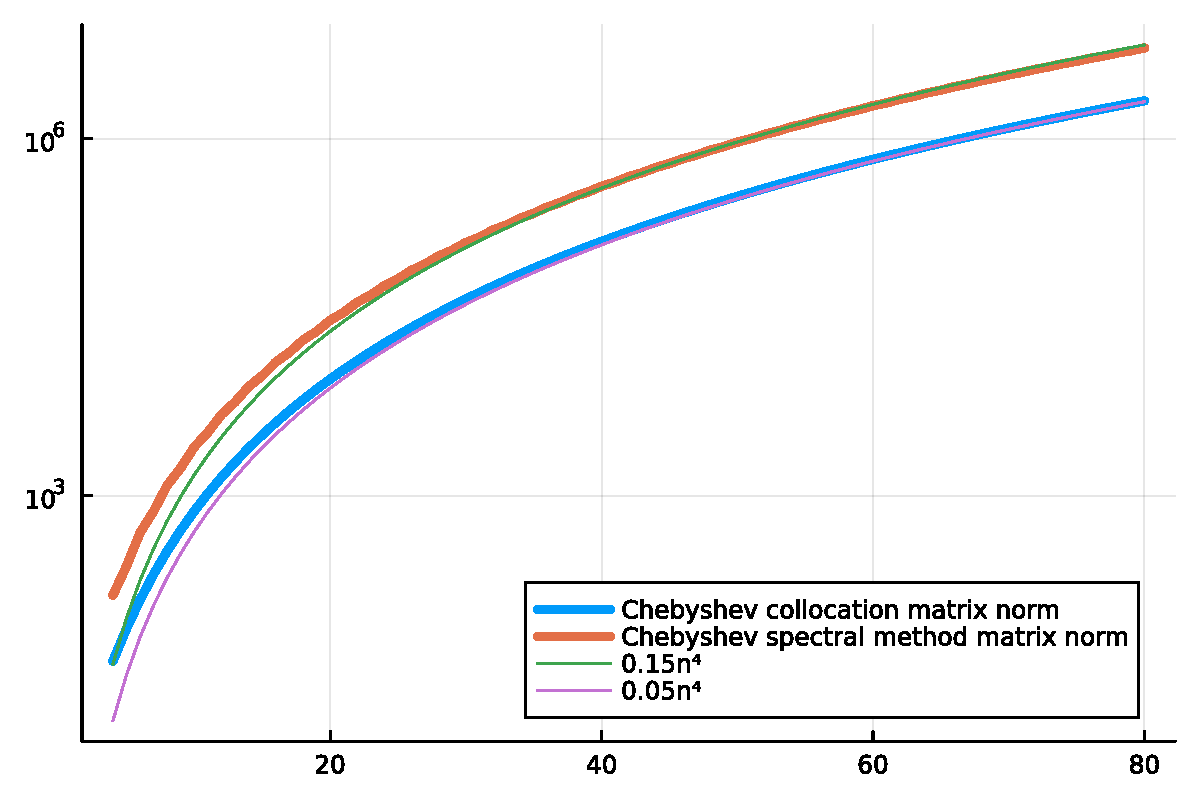
\includegraphics[width=\linewidth]{/figures/Chapter5_60_1.pdf}

\subsection{Spectral methods from Chapters 2 \& 3 revisited}
\subsubsection{Advection equation}
In Chapter 2, we considered the variable coefficient advection equation,

\[
u_t + c(x)u_x = 0, \qquad x \in [0, 2\pi), \qquad t \in [0, T],
\]
with 

\[
c(x) = \frac{1}{5} + \sin^2(x-1)
\]
and the initial data  $u(x,0) = f(x) = {\rm e}^{-100(x-1)^2}$. Since the initial data decay  rapidly to zero away from $x = 1$, we approximated the solution in the $x$ direction with a periodic trigonometric interpolant and we replaced the time derivative with a central difference approximation to obtain the following Fourier pseudospectral / Fourier collocation method:

\[
\mathbf{u}^{i+1} = \mathbf{u}^{i-1} - 2\tau c(\mathbf{x})\cdot \mathcal{F}^{-1}\left\lbrace {\rm i}(-m\!:\!m)\cdot\mathcal{F}\lbrace \mathbf{u}^{i} \rbrace\right\rbrace, \qquad i = 0, \ldots, n_t-1, \qquad \mathbf{u}^0 = \mathbf{f},
\]
where $\mathcal{F}$ and $\mathcal{F}^{-1}$ denote the application of the FFT and inverse FFT, the entries of $\mathbf{x} \in \mathbb{R}^{n_x}$ are $x_j$ and the entries of $\mathbf{u}^{i} \in \mathbb{R}^{n_x}$ are $u^{i}_j \approx u(x_j, t_i)$, with $x_j = jh$, $h = 2\pi/n_x$, $j = 0, \ldots, n_x -1$, $n_x = 2m + 1$ and $t_i = i\tau$, $i = 0, \ldots, n_t$ with $n_t\tau = T$.

To analyse the stability of this method, we recall from earlier in this chapter that the FFT can be diagonalised via unitary matrix, i.e., 

\[
\mathcal{F}^{-1}\left\lbrace {\rm i}(-m\!:\!m)\cdot\mathcal{F}\lbrace \mathbf{u}^{i} \rbrace\right\rbrace = 
Q_{n_x}^*P^*\Lambda PQ_{n_x} \mathbf{u}^{i}, \qquad \Lambda = {\rm i}\,\mathrm{diag}(-m, -(m-1), \ldots, 0, 1, \ldots, m).
\]
If we replace $c(\mathbf{x}) \in \mathbb{R}^{n_x}$ with $c_{\max} = \max\lbrace c(x) : x \in [0, 2\pi)\rbrace = 6/5$ and set $\mathbf{w}^{i} = PQ_{n_x}\mathbf{u}^{i}$, then the method decouples into $n_x$ scalar equations,

\[
w^{i+1}_j = w^{i-1}_j - 2{\rm i}\tau c_{\max} \lambda_j w^i_j, \qquad \lambda_j = j-m, \qquad j = 0, \ldots, n_x-1.
\]
Using the Von Neumann method of stability analysis, we use the ansatz $w_j^i = \rho^i {\rm e}^{{\rm i}kx_j}$ and conclude that

\[
\rho - \rho^{-1} = -2i\tau c_{max}\lambda_j
\]
Call the solutions to this equation $\rho_+$ and $\rho_-$. Note that if $\rho_+$ satisfies this equation, then so does $-\rho^{-1}_+$, which implies that $\rho_- = -\rho_+^{-1}$. For the method to be stable, it is necessary and sufficient that $\vert \rho_{\pm} \vert \leq 1$ and if $\vert \rho_{\pm} \vert = 1$, we additionally require that $\rho_{+} \neq \rho_{-}$ (this is known as the root condition, see \emph{A First Course in the Numerical Analysis of Differential Equations} by A. Iserles, p. 25).  If $\vert \rho_+ \vert < 1$, then $\vert \rho_- \vert > 1$, therefore we require $\vert \rho_+ \vert = 1$ and $\rho_+ \neq \rho_- = -\rho_+^{-1}$, i.e., $\rho_+ \neq \pm i$.

Using the quadratic formula, it follows that

\[
\rho_{\pm} = -{\rm i}\tau c_{\max} \lambda_j \pm \left(-\tau^2 c^2_{\max}\lambda_j^2 + 1   \right)^{1/2}
\]
and hence the method will be stable if and only if $\tau^2 c_{\max}^2 \lambda^2_j < 1$ or 

\[
\tau < \min_{j = 0, \ldots, n_x-1} \left\lbrace \frac{ 1}{c_{\max}\vert\lambda_j\vert}\right\rbrace = \frac{ 1}{c_{\max}m} = \frac{2}{c_{\max}(n-1)},
\]
because then

\[
\vert \rho_{\pm} \vert^2 = 1, \qquad \rho_+ \neq \rho_-.
\]
If there's a $j$ such that $\tau^2 c_{\max}^2 \lambda_j^2 \geq 1$, then these conditions are not satisfied.

Let's test the upper bound on the step size with $c(x) = 1$. First, we determine how many approximate Fourier coefficients we need to resolve the initial data to machine precision accuracy:


\begin{lstlisting}
(*@\HLJLn{n\ensuremath{\_x}}@*) (*@\HLJLoB{=}@*) (*@\HLJLni{301}@*)
(*@\HLJLn{m}@*) (*@\HLJLoB{=}@*) (*@\HLJLp{(}@*)(*@\HLJLn{n\ensuremath{\_x}}@*)(*@\HLJLoB{-}@*)(*@\HLJLni{1}@*)(*@\HLJLp{)}@*)(*@\HLJLoB{\ensuremath{\div}}@*)(*@\HLJLni{2}@*)
(*@\HLJLn{f}@*) (*@\HLJLoB{=}@*) (*@\HLJLn{x}@*) (*@\HLJLoB{->}@*) (*@\HLJLnf{exp}@*)(*@\HLJLp{(}@*)(*@\HLJLoB{-}@*)(*@\HLJLni{100}@*)(*@\HLJLoB{*}@*)(*@\HLJLp{(}@*)(*@\HLJLn{x}@*)(*@\HLJLoB{-}@*)(*@\HLJLni{1}@*)(*@\HLJLp{)}@*)(*@\HLJLoB{{\textasciicircum}}@*)(*@\HLJLni{2}@*)(*@\HLJLp{)}@*)
(*@\HLJLn{x}@*) (*@\HLJLoB{=}@*) (*@\HLJLnf{range}@*)(*@\HLJLp{(}@*)(*@\HLJLni{0}@*)(*@\HLJLp{,}@*)(*@\HLJLni{2}@*)(*@\HLJLn{\ensuremath{\pi}}@*)(*@\HLJLp{;}@*)(*@\HLJLn{length}@*)(*@\HLJLoB{=}@*)(*@\HLJLn{n\ensuremath{\_x}}@*)(*@\HLJLoB{+}@*)(*@\HLJLni{1}@*)(*@\HLJLp{)[}@*)(*@\HLJLni{1}@*)(*@\HLJLoB{:}@*)(*@\HLJLk{end}@*)(*@\HLJLoB{-}@*)(*@\HLJLni{1}@*)(*@\HLJLp{]}@*)
(*@\HLJLn{c}@*) (*@\HLJLoB{=}@*) (*@\HLJLnf{fftshift}@*)(*@\HLJLp{(}@*)(*@\HLJLnf{fft}@*)(*@\HLJLp{(}@*)(*@\HLJLn{f}@*)(*@\HLJLoB{.}@*)(*@\HLJLp{(}@*)(*@\HLJLn{x}@*)(*@\HLJLp{)))}@*)(*@\HLJLoB{/}@*)(*@\HLJLn{n\ensuremath{\_x}}@*)
(*@\HLJLnf{scatter}@*)(*@\HLJLp{(}@*)(*@\HLJLoB{-}@*)(*@\HLJLn{m}@*)(*@\HLJLoB{:}@*)(*@\HLJLn{m}@*)(*@\HLJLp{,}@*)(*@\HLJLn{abs}@*)(*@\HLJLoB{.}@*)(*@\HLJLp{(}@*)(*@\HLJLn{c}@*)(*@\HLJLp{);}@*)(*@\HLJLn{yscale}@*)(*@\HLJLoB{=:}@*)(*@\HLJLn{log10}@*)(*@\HLJLp{,}@*)(*@\HLJLn{legend}@*)(*@\HLJLoB{=}@*)(*@\HLJLkc{false}@*)(*@\HLJLp{)}@*)
\end{lstlisting}

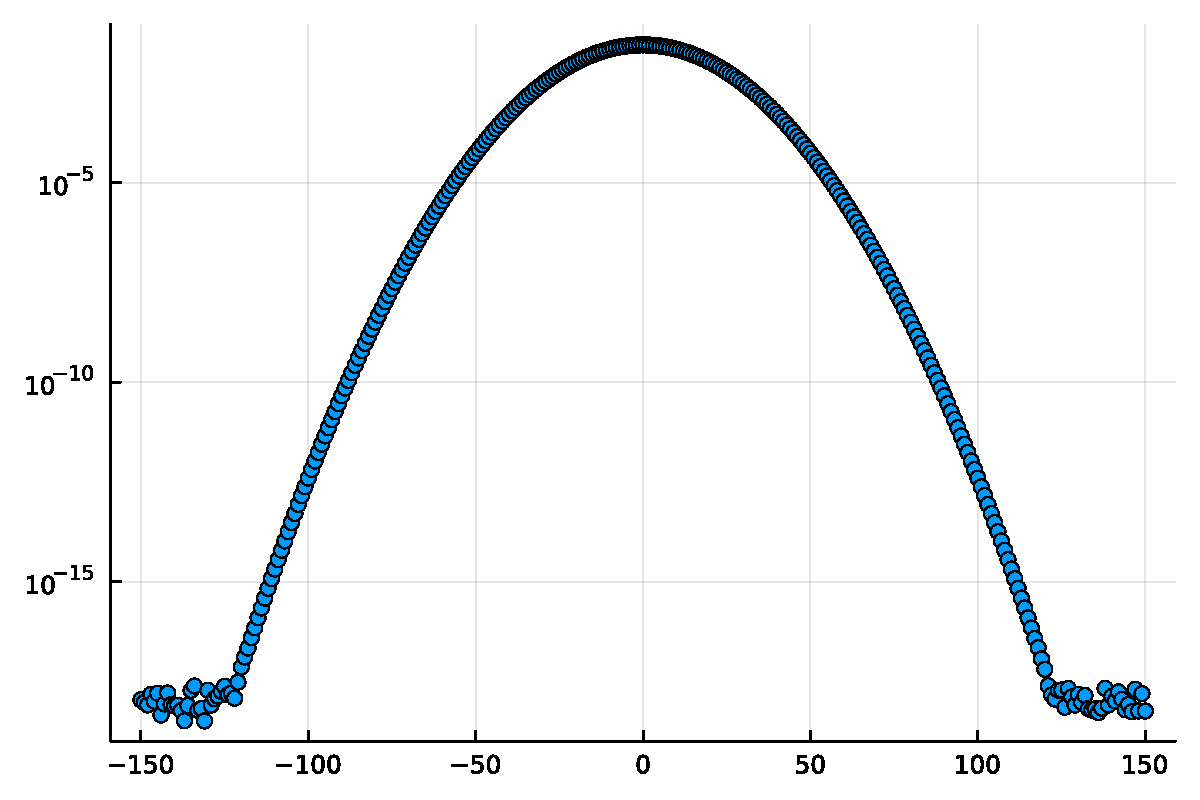
\includegraphics[width=\linewidth]{/figures/Chapter5_61_1.pdf}

\begin{lstlisting}
(*@\HLJLn{T}@*) (*@\HLJLoB{=}@*) (*@\HLJLni{2}@*)
(*@\HLJLn{cmax}@*) (*@\HLJLoB{=}@*) (*@\HLJLni{1}@*)
(*@\HLJLn{\ensuremath{\tau}}@*) (*@\HLJLoB{=}@*) (*@\HLJLnd{@show}@*) (*@\HLJLni{1}@*)(*@\HLJLoB{/}@*)(*@\HLJLp{(}@*)(*@\HLJLn{cmax}@*)(*@\HLJLoB{*}@*)(*@\HLJLn{m}@*)(*@\HLJLp{)}@*)(*@\HLJLoB{+}@*)(*@\HLJLnfB{1e-4}@*)
(*@\HLJLn{t}@*) (*@\HLJLoB{=}@*) (*@\HLJLni{0}@*)(*@\HLJLoB{:}@*)(*@\HLJLn{\ensuremath{\tau}}@*)(*@\HLJLoB{:}@*)(*@\HLJLn{T}@*)
(*@\HLJLn{n\ensuremath{\_t}}@*) (*@\HLJLoB{=}@*) (*@\HLJLnd{@show}@*) (*@\HLJLnf{length}@*)(*@\HLJLp{(}@*)(*@\HLJLn{t}@*)(*@\HLJLp{)}@*)(*@\HLJLoB{-}@*)(*@\HLJLni{1}@*)
(*@\HLJLn{u}@*) (*@\HLJLoB{=}@*) (*@\HLJLnf{zeros}@*)(*@\HLJLp{(}@*)(*@\HLJLn{n\ensuremath{\_t}}@*) (*@\HLJLoB{+}@*) (*@\HLJLni{2}@*)(*@\HLJLp{,}@*)(*@\HLJLn{n\ensuremath{\_x}}@*)(*@\HLJLp{)}@*)
(*@\HLJLn{u}@*)(*@\HLJLp{[}@*)(*@\HLJLni{2}@*)(*@\HLJLp{,}@*)(*@\HLJLoB{:}@*)(*@\HLJLp{]}@*) (*@\HLJLoB{=}@*) (*@\HLJLn{f}@*)(*@\HLJLoB{.}@*)(*@\HLJLp{(}@*)(*@\HLJLn{x}@*)(*@\HLJLp{)}@*)  (*@\HLJLcs{{\#}}@*) (*@\HLJLcs{initial}@*) (*@\HLJLcs{data}@*)
(*@\HLJLn{u}@*)(*@\HLJLp{[}@*)(*@\HLJLni{1}@*)(*@\HLJLp{,}@*)(*@\HLJLoB{:}@*)(*@\HLJLp{]}@*) (*@\HLJLoB{=}@*) (*@\HLJLn{f}@*)(*@\HLJLoB{.}@*)(*@\HLJLp{(}@*)(*@\HLJLn{x}@*) (*@\HLJLoB{.+}@*) (*@\HLJLn{\ensuremath{\tau}}@*)(*@\HLJLp{)}@*)
(*@\HLJLk{for}@*) (*@\HLJLn{n}@*) (*@\HLJLoB{=}@*) (*@\HLJLni{2}@*)(*@\HLJLoB{:}@*)(*@\HLJLn{n\ensuremath{\_t}}@*)
    (*@\HLJLn{u}@*)(*@\HLJLp{[}@*)(*@\HLJLn{n}@*)(*@\HLJLoB{+}@*)(*@\HLJLni{1}@*)(*@\HLJLp{,}@*)(*@\HLJLoB{:}@*)(*@\HLJLp{]}@*) (*@\HLJLoB{=}@*) (*@\HLJLn{real}@*)(*@\HLJLoB{.}@*)(*@\HLJLp{(}@*)(*@\HLJLn{u}@*)(*@\HLJLp{[}@*)(*@\HLJLn{n}@*)(*@\HLJLoB{-}@*)(*@\HLJLni{1}@*)(*@\HLJLp{,}@*)(*@\HLJLoB{:}@*)(*@\HLJLp{]}@*) (*@\HLJLoB{-}@*) (*@\HLJLni{2}@*)(*@\HLJLn{\ensuremath{\tau}}@*)(*@\HLJLoB{*}@*)(*@\HLJLnf{ifft}@*)(*@\HLJLp{(}@*)(*@\HLJLnf{ifftshift}@*)(*@\HLJLp{(}@*)(*@\HLJLn{im}@*)(*@\HLJLoB{*}@*)(*@\HLJLp{(}@*)(*@\HLJLoB{-}@*)(*@\HLJLn{m}@*)(*@\HLJLoB{:}@*)(*@\HLJLn{m}@*)(*@\HLJLp{))}@*)(*@\HLJLoB{.*}@*)(*@\HLJLnf{fft}@*)(*@\HLJLp{(}@*)(*@\HLJLn{u}@*)(*@\HLJLp{[}@*)(*@\HLJLn{n}@*)(*@\HLJLp{,}@*)(*@\HLJLoB{:}@*)(*@\HLJLp{])))}@*)
(*@\HLJLk{end}@*)
\end{lstlisting}

\begin{lstlisting}
1 / (cmax * m) + 0.0001 = 0.006766666666666667
length(t) - 1 = 295
\end{lstlisting}


\begin{lstlisting}
(*@\HLJLnd{@gif}@*) (*@\HLJLk{for}@*) (*@\HLJLn{i}@*) (*@\HLJLoB{=}@*) (*@\HLJLni{2}@*)(*@\HLJLoB{:}@*)(*@\HLJLni{2}@*)(*@\HLJLoB{:}@*)(*@\HLJLn{n\ensuremath{\_t}}@*)(*@\HLJLoB{+}@*)(*@\HLJLni{1}@*)
    (*@\HLJLnf{plot}@*)(*@\HLJLp{(}@*)(*@\HLJLn{x}@*)(*@\HLJLp{,}@*) (*@\HLJLn{u}@*)(*@\HLJLp{[}@*)(*@\HLJLni{2}@*)(*@\HLJLp{,}@*)(*@\HLJLoB{:}@*)(*@\HLJLp{],}@*) (*@\HLJLn{size}@*) (*@\HLJLoB{=}@*) (*@\HLJLp{(}@*)(*@\HLJLni{700}@*)(*@\HLJLp{,}@*) (*@\HLJLni{150}@*)(*@\HLJLp{),}@*) (*@\HLJLn{label}@*) (*@\HLJLoB{=}@*) (*@\HLJLs{"{}u0"{}}@*)(*@\HLJLp{)}@*)
    (*@\HLJLnf{plot!}@*)(*@\HLJLp{(}@*)(*@\HLJLn{x}@*)(*@\HLJLp{,}@*) (*@\HLJLn{f}@*)(*@\HLJLoB{.}@*)(*@\HLJLp{(}@*)(*@\HLJLn{x}@*) (*@\HLJLoB{.-}@*) (*@\HLJLnf{mod2pi}@*)(*@\HLJLp{((}@*)(*@\HLJLn{i}@*)(*@\HLJLoB{-}@*)(*@\HLJLni{1}@*)(*@\HLJLp{)}@*)(*@\HLJLoB{*}@*)(*@\HLJLn{\ensuremath{\tau}}@*)(*@\HLJLoB{*}@*)(*@\HLJLn{cmax}@*)(*@\HLJLp{)),}@*) (*@\HLJLn{lw}@*)(*@\HLJLoB{=}@*)(*@\HLJLni{2}@*)(*@\HLJLp{,}@*) (*@\HLJLn{size}@*) (*@\HLJLoB{=}@*) (*@\HLJLp{(}@*)(*@\HLJLni{700}@*)(*@\HLJLp{,}@*) (*@\HLJLni{150}@*)(*@\HLJLp{),}@*)(*@\HLJLn{label}@*)(*@\HLJLoB{=}@*)(*@\HLJLs{"{}exact}@*) (*@\HLJLs{solution"{}}@*)(*@\HLJLp{)}@*)
    (*@\HLJLnf{plot!}@*)(*@\HLJLp{(}@*)(*@\HLJLn{x}@*)(*@\HLJLp{,}@*) (*@\HLJLn{u}@*)(*@\HLJLp{[}@*)(*@\HLJLn{i}@*)(*@\HLJLp{,}@*)(*@\HLJLoB{:}@*)(*@\HLJLp{],}@*) (*@\HLJLn{label}@*) (*@\HLJLoB{=}@*) (*@\HLJLs{"{}Fourier}@*) (*@\HLJLs{pseudospectral}@*) (*@\HLJLs{method,t}@*) (*@\HLJLs{=}@*) (*@\HLJLs{"{}}@*) (*@\HLJLoB{*}@*) (*@\HLJLp{(}@*)(*@\HLJLnd{@sprintf}@*)(*@\HLJLp{(}@*)(*@\HLJLs{"{}{\%}.4f"{}}@*)(*@\HLJLp{,}@*) (*@\HLJLn{t}@*)(*@\HLJLp{[}@*)(*@\HLJLn{i}@*)(*@\HLJLp{])),}@*) (*@\HLJLn{legend}@*) (*@\HLJLoB{=}@*) (*@\HLJLsc{:outertopright}@*)(*@\HLJLp{)}@*)
(*@\HLJLk{end}@*)
\end{lstlisting}

\begin{lstlisting}
Plots.AnimatedGif((*@{"{}}@*)C:(*@{{\textbackslash}}@*)(*@{{\textbackslash}}@*)Users(*@{{\textbackslash}}@*)(*@{{\textbackslash}}@*)mfaso(*@{{\textbackslash}}@*)(*@{{\textbackslash}}@*)AppData(*@{{\textbackslash}}@*)(*@{{\textbackslash}}@*)Local(*@{{\textbackslash}}@*)(*@{{\textbackslash}}@*)Temp(*@{{\textbackslash}}@*)(*@{{\textbackslash}}@*)jl(*@{{\_}}@*)UwEqGDz2Od.gi
f(*@{"{}}@*))
\end{lstlisting}


\begin{lstlisting}
(*@\HLJLn{\ensuremath{\tau}}@*) (*@\HLJLoB{-=}@*) (*@\HLJLnfB{2E-4}@*)
(*@\HLJLn{T}@*) (*@\HLJLoB{=}@*) (*@\HLJLni{2}@*)(*@\HLJLn{\ensuremath{\pi}}@*)
(*@\HLJLn{t}@*) (*@\HLJLoB{=}@*) (*@\HLJLni{0}@*)(*@\HLJLoB{:}@*)(*@\HLJLn{\ensuremath{\tau}}@*)(*@\HLJLoB{:}@*)(*@\HLJLn{T}@*)
(*@\HLJLn{n\ensuremath{\_t}}@*) (*@\HLJLoB{=}@*) (*@\HLJLnd{@show}@*) (*@\HLJLnf{length}@*)(*@\HLJLp{(}@*)(*@\HLJLn{t}@*)(*@\HLJLp{)}@*)(*@\HLJLoB{-}@*)(*@\HLJLni{1}@*)
(*@\HLJLnd{@show}@*) (*@\HLJLn{\ensuremath{\tau}}@*)
(*@\HLJLn{u}@*) (*@\HLJLoB{=}@*) (*@\HLJLnf{zeros}@*)(*@\HLJLp{(}@*)(*@\HLJLn{n\ensuremath{\_t}}@*) (*@\HLJLoB{+}@*) (*@\HLJLni{2}@*)(*@\HLJLp{,}@*)(*@\HLJLn{n\ensuremath{\_x}}@*)(*@\HLJLp{)}@*)
(*@\HLJLn{u}@*)(*@\HLJLp{[}@*)(*@\HLJLni{2}@*)(*@\HLJLp{,}@*)(*@\HLJLoB{:}@*)(*@\HLJLp{]}@*) (*@\HLJLoB{=}@*) (*@\HLJLn{f}@*)(*@\HLJLoB{.}@*)(*@\HLJLp{(}@*)(*@\HLJLn{x}@*)(*@\HLJLp{)}@*)  (*@\HLJLcs{{\#}}@*) (*@\HLJLcs{initial}@*) (*@\HLJLcs{data}@*)
(*@\HLJLn{u}@*)(*@\HLJLp{[}@*)(*@\HLJLni{1}@*)(*@\HLJLp{,}@*)(*@\HLJLoB{:}@*)(*@\HLJLp{]}@*) (*@\HLJLoB{=}@*) (*@\HLJLn{f}@*)(*@\HLJLoB{.}@*)(*@\HLJLp{(}@*)(*@\HLJLn{x}@*) (*@\HLJLoB{.+}@*) (*@\HLJLn{\ensuremath{\tau}}@*)(*@\HLJLp{)}@*)
(*@\HLJLk{for}@*) (*@\HLJLn{n}@*) (*@\HLJLoB{=}@*) (*@\HLJLni{2}@*)(*@\HLJLoB{:}@*)(*@\HLJLn{n\ensuremath{\_t}}@*)
    (*@\HLJLn{u}@*)(*@\HLJLp{[}@*)(*@\HLJLn{n}@*)(*@\HLJLoB{+}@*)(*@\HLJLni{1}@*)(*@\HLJLp{,}@*)(*@\HLJLoB{:}@*)(*@\HLJLp{]}@*) (*@\HLJLoB{=}@*) (*@\HLJLn{real}@*)(*@\HLJLoB{.}@*)(*@\HLJLp{(}@*)(*@\HLJLn{u}@*)(*@\HLJLp{[}@*)(*@\HLJLn{n}@*)(*@\HLJLoB{-}@*)(*@\HLJLni{1}@*)(*@\HLJLp{,}@*)(*@\HLJLoB{:}@*)(*@\HLJLp{]}@*) (*@\HLJLoB{-}@*) (*@\HLJLni{2}@*)(*@\HLJLn{\ensuremath{\tau}}@*)(*@\HLJLoB{*}@*)(*@\HLJLnf{ifft}@*)(*@\HLJLp{(}@*)(*@\HLJLnf{ifftshift}@*)(*@\HLJLp{(}@*)(*@\HLJLn{im}@*)(*@\HLJLoB{*}@*)(*@\HLJLp{(}@*)(*@\HLJLoB{-}@*)(*@\HLJLn{m}@*)(*@\HLJLoB{:}@*)(*@\HLJLn{m}@*)(*@\HLJLp{))}@*)(*@\HLJLoB{.*}@*)(*@\HLJLnf{fft}@*)(*@\HLJLp{(}@*)(*@\HLJLn{u}@*)(*@\HLJLp{[}@*)(*@\HLJLn{n}@*)(*@\HLJLp{,}@*)(*@\HLJLoB{:}@*)(*@\HLJLp{])))}@*)
(*@\HLJLk{end}@*)
\end{lstlisting}

\begin{lstlisting}
length(t) - 1 = 956
(*@\ensuremath{\tau}@*) = 0.006566666666666668
\end{lstlisting}


\begin{lstlisting}
(*@\HLJLnd{@gif}@*) (*@\HLJLk{for}@*) (*@\HLJLn{i}@*) (*@\HLJLoB{=}@*) (*@\HLJLni{2}@*)(*@\HLJLoB{:}@*)(*@\HLJLni{10}@*)(*@\HLJLoB{:}@*)(*@\HLJLn{n\ensuremath{\_t}}@*)(*@\HLJLoB{+}@*)(*@\HLJLni{1}@*)
    (*@\HLJLnf{plot}@*)(*@\HLJLp{(}@*)(*@\HLJLn{x}@*)(*@\HLJLp{,}@*) (*@\HLJLn{u}@*)(*@\HLJLp{[}@*)(*@\HLJLni{2}@*)(*@\HLJLp{,}@*)(*@\HLJLoB{:}@*)(*@\HLJLp{],}@*) (*@\HLJLn{size}@*) (*@\HLJLoB{=}@*) (*@\HLJLp{(}@*)(*@\HLJLni{700}@*)(*@\HLJLp{,}@*) (*@\HLJLni{150}@*)(*@\HLJLp{),}@*) (*@\HLJLn{label}@*) (*@\HLJLoB{=}@*) (*@\HLJLs{"{}u0"{}}@*)(*@\HLJLp{)}@*)
    (*@\HLJLnf{plot!}@*)(*@\HLJLp{(}@*)(*@\HLJLn{x}@*)(*@\HLJLp{,}@*) (*@\HLJLn{f}@*)(*@\HLJLoB{.}@*)(*@\HLJLp{(}@*)(*@\HLJLn{mod2pi}@*)(*@\HLJLoB{.}@*)(*@\HLJLp{(}@*)(*@\HLJLn{x}@*) (*@\HLJLoB{.-}@*) (*@\HLJLp{(}@*)(*@\HLJLn{i}@*)(*@\HLJLoB{-}@*)(*@\HLJLni{1}@*)(*@\HLJLp{)}@*)(*@\HLJLoB{*}@*)(*@\HLJLn{\ensuremath{\tau}}@*)(*@\HLJLoB{*}@*)(*@\HLJLn{cmax}@*)(*@\HLJLp{)),}@*) (*@\HLJLn{lw}@*)(*@\HLJLoB{=}@*)(*@\HLJLni{2}@*)(*@\HLJLp{,}@*) (*@\HLJLn{size}@*) (*@\HLJLoB{=}@*) (*@\HLJLp{(}@*)(*@\HLJLni{700}@*)(*@\HLJLp{,}@*) (*@\HLJLni{150}@*)(*@\HLJLp{),}@*)(*@\HLJLn{label}@*)(*@\HLJLoB{=}@*)(*@\HLJLs{"{}exact}@*) (*@\HLJLs{solution"{}}@*)(*@\HLJLp{)}@*)
    (*@\HLJLnf{plot!}@*)(*@\HLJLp{(}@*)(*@\HLJLn{x}@*)(*@\HLJLp{,}@*) (*@\HLJLn{u}@*)(*@\HLJLp{[}@*)(*@\HLJLn{i}@*)(*@\HLJLp{,}@*)(*@\HLJLoB{:}@*)(*@\HLJLp{],}@*) (*@\HLJLn{label}@*) (*@\HLJLoB{=}@*) (*@\HLJLs{"{}Fourier}@*) (*@\HLJLs{pseudospectral}@*) (*@\HLJLs{method,t}@*) (*@\HLJLs{=}@*) (*@\HLJLs{"{}}@*) (*@\HLJLoB{*}@*) (*@\HLJLp{(}@*)(*@\HLJLnd{@sprintf}@*)(*@\HLJLp{(}@*)(*@\HLJLs{"{}{\%}.4f"{}}@*)(*@\HLJLp{,}@*) (*@\HLJLn{t}@*)(*@\HLJLp{[}@*)(*@\HLJLn{i}@*)(*@\HLJLp{])),}@*) (*@\HLJLn{legend}@*) (*@\HLJLoB{=}@*) (*@\HLJLsc{:outertopright}@*)(*@\HLJLp{)}@*)
(*@\HLJLk{end}@*)
\end{lstlisting}

\begin{lstlisting}
Plots.AnimatedGif((*@{"{}}@*)C:(*@{{\textbackslash}}@*)(*@{{\textbackslash}}@*)Users(*@{{\textbackslash}}@*)(*@{{\textbackslash}}@*)mfaso(*@{{\textbackslash}}@*)(*@{{\textbackslash}}@*)AppData(*@{{\textbackslash}}@*)(*@{{\textbackslash}}@*)Local(*@{{\textbackslash}}@*)(*@{{\textbackslash}}@*)Temp(*@{{\textbackslash}}@*)(*@{{\textbackslash}}@*)jl(*@{{\_}}@*)e4SrEhO1oJ.gi
f(*@{"{}}@*))
\end{lstlisting}


Now let's consider the case when $c(x) = 1/5 + \sin^2(x-1)$


\begin{lstlisting}
(*@\HLJLn{c}@*) (*@\HLJLoB{=}@*) (*@\HLJLn{x}@*) (*@\HLJLoB{->}@*) (*@\HLJLnfB{0.2}@*) (*@\HLJLoB{+}@*) (*@\HLJLnf{sin}@*)(*@\HLJLp{(}@*)(*@\HLJLn{x}@*) (*@\HLJLoB{-}@*) (*@\HLJLni{1}@*)(*@\HLJLp{)}@*)(*@\HLJLoB{{\textasciicircum}}@*)(*@\HLJLni{2}@*)
(*@\HLJLn{n\ensuremath{\_x}}@*) (*@\HLJLoB{=}@*) (*@\HLJLni{401}@*)
(*@\HLJLn{cmax}@*) (*@\HLJLoB{=}@*) (*@\HLJLni{6}@*)(*@\HLJLoB{/}@*)(*@\HLJLni{5}@*)
(*@\HLJLn{m}@*) (*@\HLJLoB{=}@*) (*@\HLJLp{(}@*)(*@\HLJLn{n\ensuremath{\_x}}@*)(*@\HLJLoB{-}@*)(*@\HLJLni{1}@*)(*@\HLJLp{)}@*)(*@\HLJLoB{\ensuremath{\div}}@*)(*@\HLJLni{2}@*)
(*@\HLJLn{x}@*) (*@\HLJLoB{=}@*) (*@\HLJLnf{range}@*)(*@\HLJLp{(}@*)(*@\HLJLni{0}@*)(*@\HLJLp{,}@*)(*@\HLJLni{2}@*)(*@\HLJLn{\ensuremath{\pi}}@*)(*@\HLJLp{;}@*)(*@\HLJLn{length}@*)(*@\HLJLoB{=}@*)(*@\HLJLn{n\ensuremath{\_x}}@*)(*@\HLJLoB{+}@*)(*@\HLJLni{1}@*)(*@\HLJLp{)[}@*)(*@\HLJLni{1}@*)(*@\HLJLoB{:}@*)(*@\HLJLk{end}@*)(*@\HLJLoB{-}@*)(*@\HLJLni{1}@*)(*@\HLJLp{]}@*) 
(*@\HLJLn{\ensuremath{\tau}}@*) (*@\HLJLoB{=}@*) (*@\HLJLnd{@show}@*) (*@\HLJLni{1}@*)(*@\HLJLoB{/}@*)(*@\HLJLp{(}@*)(*@\HLJLn{m}@*)(*@\HLJLoB{*}@*)(*@\HLJLn{cmax}@*)(*@\HLJLp{)}@*)
(*@\HLJLn{\ensuremath{\tau}}@*) (*@\HLJLoB{=}@*) (*@\HLJLnfB{0.0044}@*) (*@\HLJLcs{{\#}}@*) (*@\HLJLcs{no}@*) (*@\HLJLcs{blow}@*) (*@\HLJLcs{up}@*)
(*@\HLJLcs{{\#}\ensuremath{\tau}}@*) (*@\HLJLcs{=}@*) (*@\HLJLcs{0.00441}@*) (*@\HLJLcs{{\#}blow}@*) (*@\HLJLcs{up}@*)
(*@\HLJLn{T}@*) (*@\HLJLoB{=}@*) (*@\HLJLnfB{12.825}@*)
(*@\HLJLn{t}@*) (*@\HLJLoB{=}@*) (*@\HLJLni{0}@*)(*@\HLJLoB{:}@*)(*@\HLJLn{\ensuremath{\tau}}@*)(*@\HLJLoB{:}@*)(*@\HLJLn{T}@*)
(*@\HLJLn{n\ensuremath{\_t}}@*) (*@\HLJLoB{=}@*) (*@\HLJLnd{@show}@*) (*@\HLJLnf{length}@*)(*@\HLJLp{(}@*)(*@\HLJLn{t}@*)(*@\HLJLp{)}@*)(*@\HLJLoB{-}@*)(*@\HLJLni{1}@*)
(*@\HLJLn{u}@*) (*@\HLJLoB{=}@*) (*@\HLJLnf{zeros}@*)(*@\HLJLp{(}@*)(*@\HLJLn{n\ensuremath{\_t}}@*) (*@\HLJLoB{+}@*) (*@\HLJLni{2}@*)(*@\HLJLp{,}@*)(*@\HLJLn{n\ensuremath{\_x}}@*)(*@\HLJLp{)}@*)
(*@\HLJLn{u}@*)(*@\HLJLp{[}@*)(*@\HLJLni{2}@*)(*@\HLJLp{,}@*)(*@\HLJLoB{:}@*)(*@\HLJLp{]}@*) (*@\HLJLoB{=}@*) (*@\HLJLn{f}@*)(*@\HLJLoB{.}@*)(*@\HLJLp{(}@*)(*@\HLJLn{x}@*)(*@\HLJLp{)}@*) 
(*@\HLJLn{u}@*)(*@\HLJLp{[}@*)(*@\HLJLni{1}@*)(*@\HLJLp{,}@*)(*@\HLJLoB{:}@*)(*@\HLJLp{]}@*) (*@\HLJLoB{=}@*) (*@\HLJLn{f}@*)(*@\HLJLoB{.}@*)(*@\HLJLp{(}@*)(*@\HLJLn{x}@*) (*@\HLJLoB{.+}@*) (*@\HLJLnfB{0.2}@*)(*@\HLJLoB{*}@*)(*@\HLJLn{\ensuremath{\tau}}@*)(*@\HLJLp{)}@*)

(*@\HLJLk{for}@*) (*@\HLJLn{n}@*) (*@\HLJLoB{=}@*) (*@\HLJLni{2}@*)(*@\HLJLoB{:}@*)(*@\HLJLn{n\ensuremath{\_t}}@*)(*@\HLJLoB{-}@*)(*@\HLJLni{1}@*)
    (*@\HLJLn{u}@*)(*@\HLJLp{[}@*)(*@\HLJLn{n}@*)(*@\HLJLoB{+}@*)(*@\HLJLni{1}@*)(*@\HLJLp{,}@*)(*@\HLJLoB{:}@*)(*@\HLJLp{]}@*) (*@\HLJLoB{=}@*) (*@\HLJLn{real}@*)(*@\HLJLoB{.}@*)(*@\HLJLp{(}@*)(*@\HLJLn{u}@*)(*@\HLJLp{[}@*)(*@\HLJLn{n}@*)(*@\HLJLoB{-}@*)(*@\HLJLni{1}@*)(*@\HLJLp{,}@*)(*@\HLJLoB{:}@*)(*@\HLJLp{]}@*) (*@\HLJLoB{-}@*) (*@\HLJLni{2}@*)(*@\HLJLn{\ensuremath{\tau}}@*)(*@\HLJLoB{*}@*)(*@\HLJLn{c}@*)(*@\HLJLoB{.}@*)(*@\HLJLp{(}@*)(*@\HLJLn{x}@*)(*@\HLJLp{)}@*)(*@\HLJLoB{.*}@*)(*@\HLJLnf{ifft}@*)(*@\HLJLp{(}@*)(*@\HLJLnf{ifftshift}@*)(*@\HLJLp{(}@*)(*@\HLJLn{im}@*)(*@\HLJLoB{*}@*)(*@\HLJLp{(}@*)(*@\HLJLoB{-}@*)(*@\HLJLn{m}@*)(*@\HLJLoB{:}@*)(*@\HLJLn{m}@*)(*@\HLJLp{))}@*)(*@\HLJLoB{.*}@*)(*@\HLJLnf{fft}@*)(*@\HLJLp{(}@*)(*@\HLJLn{u}@*)(*@\HLJLp{[}@*)(*@\HLJLn{n}@*)(*@\HLJLp{,}@*)(*@\HLJLoB{:}@*)(*@\HLJLp{])))}@*)
(*@\HLJLk{end}@*)
\end{lstlisting}

\begin{lstlisting}
1 / (m * cmax) = 0.004166666666666667
length(t) - 1 = 2914
\end{lstlisting}


\begin{lstlisting}
(*@\HLJLnd{@gif}@*) (*@\HLJLk{for}@*) (*@\HLJLn{i}@*) (*@\HLJLoB{=}@*) (*@\HLJLni{2}@*)(*@\HLJLoB{:}@*)(*@\HLJLni{20}@*)(*@\HLJLoB{:}@*)(*@\HLJLn{n\ensuremath{\_t}}@*)(*@\HLJLoB{+}@*)(*@\HLJLni{1}@*)
    (*@\HLJLnf{plot}@*)(*@\HLJLp{(}@*)(*@\HLJLn{x}@*)(*@\HLJLp{,}@*) (*@\HLJLn{u}@*)(*@\HLJLp{[}@*)(*@\HLJLni{2}@*)(*@\HLJLp{,}@*)(*@\HLJLoB{:}@*)(*@\HLJLp{],}@*) (*@\HLJLn{size}@*) (*@\HLJLoB{=}@*) (*@\HLJLp{(}@*)(*@\HLJLni{700}@*)(*@\HLJLp{,}@*) (*@\HLJLni{150}@*)(*@\HLJLp{),}@*) (*@\HLJLn{label}@*) (*@\HLJLoB{=}@*) (*@\HLJLs{"{}u0"{}}@*)(*@\HLJLp{)}@*)
    (*@\HLJLnf{plot!}@*)(*@\HLJLp{(}@*)(*@\HLJLn{x}@*)(*@\HLJLp{,}@*) (*@\HLJLn{u}@*)(*@\HLJLp{[}@*)(*@\HLJLn{i}@*)(*@\HLJLp{,}@*)(*@\HLJLoB{:}@*)(*@\HLJLp{],}@*) (*@\HLJLn{lw}@*)(*@\HLJLoB{=}@*)(*@\HLJLni{2}@*)(*@\HLJLp{,}@*) (*@\HLJLn{label}@*) (*@\HLJLoB{=}@*) (*@\HLJLs{"{}Fourier}@*) (*@\HLJLs{collocation,t}@*) (*@\HLJLs{=}@*) (*@\HLJLs{"{}}@*) (*@\HLJLoB{*}@*) (*@\HLJLp{(}@*)(*@\HLJLnd{@sprintf}@*)(*@\HLJLp{(}@*)(*@\HLJLs{"{}{\%}.4f"{}}@*)(*@\HLJLp{,}@*) (*@\HLJLn{t}@*)(*@\HLJLp{[}@*)(*@\HLJLn{i}@*)(*@\HLJLp{])),}@*) (*@\HLJLn{legend}@*) (*@\HLJLoB{=}@*) (*@\HLJLsc{:outertopright}@*)(*@\HLJLp{)}@*)
(*@\HLJLk{end}@*)
\end{lstlisting}

\begin{lstlisting}
Plots.AnimatedGif((*@{"{}}@*)C:(*@{{\textbackslash}}@*)(*@{{\textbackslash}}@*)Users(*@{{\textbackslash}}@*)(*@{{\textbackslash}}@*)mfaso(*@{{\textbackslash}}@*)(*@{{\textbackslash}}@*)AppData(*@{{\textbackslash}}@*)(*@{{\textbackslash}}@*)Local(*@{{\textbackslash}}@*)(*@{{\textbackslash}}@*)Temp(*@{{\textbackslash}}@*)(*@{{\textbackslash}}@*)jl(*@{{\_}}@*)FsK4yAPdZX.gi
f(*@{"{}}@*))
\end{lstlisting}


\begin{lstlisting}
(*@\HLJLn{\ensuremath{\tau}}@*) (*@\HLJLoB{=}@*) (*@\HLJLnfB{0.00441}@*) (*@\HLJLcs{{\#}blow}@*) (*@\HLJLcs{up}@*)
(*@\HLJLn{t}@*) (*@\HLJLoB{=}@*) (*@\HLJLni{0}@*)(*@\HLJLoB{:}@*)(*@\HLJLn{\ensuremath{\tau}}@*)(*@\HLJLoB{:}@*)(*@\HLJLn{T}@*)
(*@\HLJLn{n\ensuremath{\_t}}@*) (*@\HLJLoB{=}@*) (*@\HLJLnd{@show}@*) (*@\HLJLnf{length}@*)(*@\HLJLp{(}@*)(*@\HLJLn{t}@*)(*@\HLJLp{)}@*)(*@\HLJLoB{-}@*)(*@\HLJLni{1}@*)
(*@\HLJLn{u}@*) (*@\HLJLoB{=}@*) (*@\HLJLnf{zeros}@*)(*@\HLJLp{(}@*)(*@\HLJLn{n\ensuremath{\_t}}@*) (*@\HLJLoB{+}@*) (*@\HLJLni{2}@*)(*@\HLJLp{,}@*)(*@\HLJLn{n\ensuremath{\_x}}@*)(*@\HLJLp{)}@*)
(*@\HLJLn{u}@*)(*@\HLJLp{[}@*)(*@\HLJLni{2}@*)(*@\HLJLp{,}@*)(*@\HLJLoB{:}@*)(*@\HLJLp{]}@*) (*@\HLJLoB{=}@*) (*@\HLJLn{f}@*)(*@\HLJLoB{.}@*)(*@\HLJLp{(}@*)(*@\HLJLn{x}@*)(*@\HLJLp{)}@*) 
(*@\HLJLn{u}@*)(*@\HLJLp{[}@*)(*@\HLJLni{1}@*)(*@\HLJLp{,}@*)(*@\HLJLoB{:}@*)(*@\HLJLp{]}@*) (*@\HLJLoB{=}@*) (*@\HLJLn{f}@*)(*@\HLJLoB{.}@*)(*@\HLJLp{(}@*)(*@\HLJLn{x}@*) (*@\HLJLoB{.+}@*) (*@\HLJLnfB{0.2}@*)(*@\HLJLoB{*}@*)(*@\HLJLn{\ensuremath{\tau}}@*)(*@\HLJLp{)}@*) 
(*@\HLJLk{for}@*) (*@\HLJLn{n}@*) (*@\HLJLoB{=}@*) (*@\HLJLni{2}@*)(*@\HLJLoB{:}@*)(*@\HLJLn{n\ensuremath{\_t}}@*)(*@\HLJLoB{-}@*)(*@\HLJLni{1}@*)
    (*@\HLJLn{u}@*)(*@\HLJLp{[}@*)(*@\HLJLn{n}@*)(*@\HLJLoB{+}@*)(*@\HLJLni{1}@*)(*@\HLJLp{,}@*)(*@\HLJLoB{:}@*)(*@\HLJLp{]}@*) (*@\HLJLoB{=}@*) (*@\HLJLn{real}@*)(*@\HLJLoB{.}@*)(*@\HLJLp{(}@*)(*@\HLJLn{u}@*)(*@\HLJLp{[}@*)(*@\HLJLn{n}@*)(*@\HLJLoB{-}@*)(*@\HLJLni{1}@*)(*@\HLJLp{,}@*)(*@\HLJLoB{:}@*)(*@\HLJLp{]}@*) (*@\HLJLoB{-}@*) (*@\HLJLni{2}@*)(*@\HLJLn{\ensuremath{\tau}}@*)(*@\HLJLoB{*}@*)(*@\HLJLn{c}@*)(*@\HLJLoB{.}@*)(*@\HLJLp{(}@*)(*@\HLJLn{x}@*)(*@\HLJLp{)}@*)(*@\HLJLoB{.*}@*)(*@\HLJLnf{ifft}@*)(*@\HLJLp{(}@*)(*@\HLJLnf{ifftshift}@*)(*@\HLJLp{(}@*)(*@\HLJLn{im}@*)(*@\HLJLoB{*}@*)(*@\HLJLp{(}@*)(*@\HLJLoB{-}@*)(*@\HLJLn{m}@*)(*@\HLJLoB{:}@*)(*@\HLJLn{m}@*)(*@\HLJLp{))}@*)(*@\HLJLoB{.*}@*)(*@\HLJLnf{fft}@*)(*@\HLJLp{(}@*)(*@\HLJLn{u}@*)(*@\HLJLp{[}@*)(*@\HLJLn{n}@*)(*@\HLJLp{,}@*)(*@\HLJLoB{:}@*)(*@\HLJLp{])))}@*)
(*@\HLJLk{end}@*)
\end{lstlisting}

\begin{lstlisting}
length(t) - 1 = 2908
\end{lstlisting}


\begin{lstlisting}
(*@\HLJLnd{@gif}@*) (*@\HLJLk{for}@*) (*@\HLJLn{i}@*) (*@\HLJLoB{=}@*) (*@\HLJLni{2}@*)(*@\HLJLoB{:}@*)(*@\HLJLni{20}@*)(*@\HLJLoB{:}@*)(*@\HLJLn{n\ensuremath{\_t}}@*)(*@\HLJLoB{+}@*)(*@\HLJLni{1}@*)
    (*@\HLJLnf{plot}@*)(*@\HLJLp{(}@*)(*@\HLJLn{x}@*)(*@\HLJLp{,}@*) (*@\HLJLn{u}@*)(*@\HLJLp{[}@*)(*@\HLJLni{2}@*)(*@\HLJLp{,}@*)(*@\HLJLoB{:}@*)(*@\HLJLp{],}@*) (*@\HLJLn{size}@*) (*@\HLJLoB{=}@*) (*@\HLJLp{(}@*)(*@\HLJLni{700}@*)(*@\HLJLp{,}@*) (*@\HLJLni{150}@*)(*@\HLJLp{),}@*) (*@\HLJLn{label}@*) (*@\HLJLoB{=}@*) (*@\HLJLs{"{}u0"{}}@*)(*@\HLJLp{)}@*)
    (*@\HLJLnf{plot!}@*)(*@\HLJLp{(}@*)(*@\HLJLn{x}@*)(*@\HLJLp{,}@*) (*@\HLJLn{u}@*)(*@\HLJLp{[}@*)(*@\HLJLn{i}@*)(*@\HLJLp{,}@*)(*@\HLJLoB{:}@*)(*@\HLJLp{],}@*) (*@\HLJLn{lw}@*)(*@\HLJLoB{=}@*)(*@\HLJLni{2}@*)(*@\HLJLp{,}@*) (*@\HLJLn{label}@*) (*@\HLJLoB{=}@*) (*@\HLJLs{"{}Fourier}@*) (*@\HLJLs{collocation,t}@*) (*@\HLJLs{=}@*) (*@\HLJLs{"{}}@*) (*@\HLJLoB{*}@*) (*@\HLJLp{(}@*)(*@\HLJLnd{@sprintf}@*)(*@\HLJLp{(}@*)(*@\HLJLs{"{}{\%}.4f"{}}@*)(*@\HLJLp{,}@*) (*@\HLJLn{t}@*)(*@\HLJLp{[}@*)(*@\HLJLn{i}@*)(*@\HLJLp{])),}@*) (*@\HLJLn{legend}@*) (*@\HLJLoB{=}@*) (*@\HLJLsc{:outertopright}@*)(*@\HLJLp{)}@*)
(*@\HLJLk{end}@*)
\end{lstlisting}

\begin{lstlisting}
Plots.AnimatedGif((*@{"{}}@*)C:(*@{{\textbackslash}}@*)(*@{{\textbackslash}}@*)Users(*@{{\textbackslash}}@*)(*@{{\textbackslash}}@*)mfaso(*@{{\textbackslash}}@*)(*@{{\textbackslash}}@*)AppData(*@{{\textbackslash}}@*)(*@{{\textbackslash}}@*)Local(*@{{\textbackslash}}@*)(*@{{\textbackslash}}@*)Temp(*@{{\textbackslash}}@*)(*@{{\textbackslash}}@*)jl(*@{{\_}}@*)sfHftCn4uf.gi
f(*@{"{}}@*))
\end{lstlisting}


\subsubsection{Wave equation}
In Chapter 3, we considered the wave equation

\[
u_{tt} = u_{xx}, \qquad t > 0, \qquad -1 < x < 1, \qquad ,
\]
subject to zero boundary conditions $u(\pm 1, t) = 0$ and the initial data

\[
u(x,0) = f(x) = {\rm e}^{-200x^2}.
\]
Rather than specifying $u_t(x,0)$, we imposed the condition

\[
u(x,-\tau) = f(x - \tau) = {\rm e}^{-200(x-\tau)^2}.
\]
We approximated the solution with a Chebyshev interpolant in $x$, i.e., 

\[
u(x,t) \approx u_{n_x}(x,t) = \sum_{k=0}^{n_x} \ell_k(x)v_k(t), \quad \ell_k(x) = \prod_{\substack{j=0\\ j \neq k}}^{n_x}\frac{x-x_j}{x_k-x_j}, \quad x_k = \cos\left(\frac{\pi k}{n_x} \right),
\]
where $u(x_j,t) \approx v_j(t)$.  Due to the zero boundary data, we set $v_0(t) = v_{n_x}(t)$. We specify that $u_{n_x}(x,t)$ satisfy the wave equation at the collocation points, i.e., 

\[
\frac{\partial^2}{\partial t^2}u_{n_x}(x_j,t) = \frac{\partial^2}{\partial x^2} u_{n_x}(x_j,t),
\]
which is equivalent to the second-order system of ODEs:


\begin{eqnarray*}
\left(
\begin{array}{c}
v_1''(t) \\
v_2''(t) \\
\vdots \\
v_{n_x-1}''(t)
\end{array}
\right) &=& 
\left(
\begin{array}{c c c c c}
\ell''_0(x_1) &\ell''_1(x_1) & \cdots &\ell''_{n_x-1}(x_1) & \ell''_{n_x}(x_1) \\
\ell''_0(x_2) &\ell''_1(x_2) & \cdots &\ell''_{n_x-1}(x_2) & \ell''_{n_x}(x_2)  \\
     \vdots  & \vdots & \vdots & \vdots & \vdots  \\
\ell''_0(x_{n_x-1}) &\ell''_1(x_{n_x-1}) & \cdots &\ell''_{n_x-1}(x_{n_x-1}) & \ell''_{n_x}(x_{n_x-1})
\end{array} 
\right)
\left(
\begin{array}{c}
v_0(t) \\
v_1(t) \\
\vdots \\
v_{n_x-1}(t) \\
v_{n_x}(t)
\end{array}
\right) \\
&=& \left(
\begin{array}{ c c c }
\ell''_1(x_1) & \cdots &\ell''_{n_x-1}(x_1)  \\
\ell''_1(x_2) & \cdots &\ell''_{n_x-1}(x_2)   \\
   \vdots & \vdots & \vdots   \\
\ell''_1(x_{n_x-1}) & \cdots &\ell''_{n_x-1}(x_{n_x-1}) 
\end{array} 
\right)
\left(
\begin{array}{c}
v_1(t) \\
\vdots \\
v_{n_x-1}(t)
\end{array}
\right)  := A\mathbf{v}(t).
\end{eqnarray*}
Note that the matrix $A$ is the same as the matrix we encountered when we solved the diffusion equation with a Chebyshev collocation method earlier in this chapter; it is the second to $n$-th columns of the second-order Chebyshev differentiation matrix.

We approximated the second time derivative with a central difference, hence we set

\[
v_j(t_i) \approx u^{i}_j, \qquad t_i = i\tau, \qquad i = 0, \ldots, n_t,
\]
and

\[
v_j''(t_i) \approx \frac{u^{i+1}_j - 2u^i_j + u^{i-1}_j}{\tau^2}.
\]
Substituting this into the second-order ODE system, we obtain the leap frog method

\[
\mathbf{u}^{i+1} = 2\mathbf{u}^{i} - \mathbf{u}^{i-1} + \tau^2 A\mathbf{u}^{i}, \qquad i = 0, \ldots, n_t-1.
\]
and from the initial data, we set

\[
\mathbf{u}^{0} = f(\mathbf{x}), \qquad \mathbf{u}^{-1} = f(\mathbf{x}-\tau).
\]
To analyse the stability of the method, we recall from earlier in this chapter that $A$ has the eigendecomposition $A = W\Lambda W^{-1}$. Setting $\mathbf{w}^i = W^{-1}\mathbf{u}^{i}$, the leap frog method becomes

\[
\mathbf{w}^{i+1} = 2\mathbf{w}^{i} - \mathbf{w}^{i-1} +  \tau^2\Lambda \mathbf{w}^{i},
\]
i.e.,

\[
w^{i+1}_j = 2w^{i}_j - w^{i-1}_j +  \tau^2\lambda_j w^{i}_j, \qquad j = 1, \ldots, n_x-1,
\]
where the $\lambda_j$ are the eigenvalues of $A$.  We learnt earlier in this chapter that the $\lambda_j$ are negative real numbers and that 

\[
\rho(A) = \max_{j = 1, \ldots, n_x-1} \lbrace \vert \lambda_j \vert  \rbrace \approx \frac{(n_x-1)^4}{20}.
\]
Using the Von Neumann method of stability analysis, we set $w^i_j = \rho^i {\rm e}^{{\rm i}kx_j}$ and find that

\[
\rho  + \rho^{-1} =  2\left(1 - \frac{\tau^2}{2} \vert \lambda_j \vert\right)
\]
Call the solutions to this equation $\rho_+$ and $\rho_-$. Note that if $\rho_+$ satisfies this equation, then so does $\rho^{-1}_+$, which implies that $\rho_- = \rho_+^{-1}$. For the method to be stable, it is necessary and sufficient that $\vert \rho_{\pm} \vert \leq 1$ and if $\vert \rho_{\pm} \vert = 1$, we additionally require that $\rho_{+} \neq \rho_{-}$.  If $\vert \rho_+ \vert < 1$, then $\vert \rho_- \vert > 1$, therefore we require $\vert \rho_+ \vert = 1$ and $\rho_+ \neq \rho_- = \rho_+^{-1}$, i.e., $\rho_+ \neq \pm 1$.

Using the quadratic formula and assuming $\tau^4\vert \lambda_j \vert^2/4 - \tau^2\vert \lambda_j \vert < 0$ or $\tau < 2/\sqrt{\vert \lambda_j \vert}$ for $j = 1, \ldots, n_x-1$, it follows that


\begin{eqnarray*}
\rho_{\pm}
&=& 1 - \frac{\tau^2}{2}\vert \lambda_j \vert  \pm i\left( \tau^2\vert \lambda_j \vert -\frac{\tau^4}{4}\vert \lambda_j \vert^2   \right)^{1/2}
\end{eqnarray*}
and hence the method is stable because $\vert \rho_{\pm} \vert^2 = 1$  and $\rho_+ \neq \rho_-$.  It also follows that if there's a $j$ such that $\tau \geq 2/\sqrt{\vert \lambda_j \vert}$, then these conditions are not satisfied and the method is unstable.

We estimate the step size restriction to be

\[
\tau < \min_{j = 1, \ldots, n_x-1}\left\lbrace \frac{2}{\sqrt{\vert \lambda_j \vert}}\right\rbrace \approx \frac{4\sqrt{5}}{(n_x-1)^2}
\]
Let's test this: First, we shall use the following function to compute the matrix-vector product $A\mathbf{u}^{i}$ via the FFT.


\begin{lstlisting}
(*@\HLJLk{function}@*) (*@\HLJLnf{chebfft}@*)(*@\HLJLp{(}@*)(*@\HLJLn{f}@*)(*@\HLJLp{)}@*)
    (*@\HLJLn{n}@*) (*@\HLJLoB{=}@*) (*@\HLJLnf{length}@*)(*@\HLJLp{(}@*)(*@\HLJLn{f}@*)(*@\HLJLp{)}@*)(*@\HLJLoB{-}@*)(*@\HLJLni{1}@*)
    (*@\HLJLn{x}@*) (*@\HLJLoB{=}@*) (*@\HLJLn{cos}@*)(*@\HLJLoB{.}@*)(*@\HLJLp{((}@*)(*@\HLJLni{0}@*)(*@\HLJLoB{:}@*)(*@\HLJLn{n}@*)(*@\HLJLp{)}@*)(*@\HLJLoB{*}@*)(*@\HLJLn{\ensuremath{\pi}}@*)(*@\HLJLoB{/}@*)(*@\HLJLn{n}@*)(*@\HLJLp{)}@*) (*@\HLJLcs{{\#}}@*) (*@\HLJLcs{Chebyshev}@*) (*@\HLJLcs{points}@*)
    (*@\HLJLn{ii}@*) (*@\HLJLoB{=}@*) (*@\HLJLni{0}@*)(*@\HLJLoB{:}@*)(*@\HLJLn{n}@*)(*@\HLJLoB{-}@*)(*@\HLJLni{1}@*)
    (*@\HLJLn{q}@*) (*@\HLJLoB{=}@*) (*@\HLJLp{[}@*)(*@\HLJLn{f}@*)(*@\HLJLp{;}@*) (*@\HLJLn{f}@*)(*@\HLJLp{[}@*)(*@\HLJLn{n}@*)(*@\HLJLoB{:-}@*)(*@\HLJLni{1}@*)(*@\HLJLoB{:}@*)(*@\HLJLni{2}@*)(*@\HLJLp{]]}@*)      (*@\HLJLcs{{\#}}@*) (*@\HLJLcs{transform}@*) (*@\HLJLcs{x}@*) (*@\HLJLcs{->}@*) (*@\HLJLcs{\ensuremath{\theta}}@*)    
    (*@\HLJLcs{{\#}}@*) (*@\HLJLcs{differentiate}@*) (*@\HLJLcs{the}@*) (*@\HLJLcs{interpolant}@*) (*@\HLJLcs{q\ensuremath{\_n}}@*) (*@\HLJLcs{in}@*) (*@\HLJLcs{coefficient}@*) (*@\HLJLcs{space}@*) (*@\HLJLcs{and}@*) (*@\HLJLcs{map}@*) (*@\HLJLcs{back}@*) (*@\HLJLcs{to}@*) (*@\HLJLcs{function}@*) (*@\HLJLcs{values}@*)
    (*@\HLJLn{cq}@*) (*@\HLJLoB{=}@*) (*@\HLJLn{real}@*)(*@\HLJLoB{.}@*)(*@\HLJLp{(}@*)(*@\HLJLnf{fft}@*)(*@\HLJLp{(}@*)(*@\HLJLn{q}@*)(*@\HLJLp{))}@*)
    (*@\HLJLn{dq}@*) (*@\HLJLoB{=}@*) (*@\HLJLn{real}@*)(*@\HLJLoB{.}@*)(*@\HLJLp{(}@*)(*@\HLJLnf{ifft}@*)(*@\HLJLp{(}@*)(*@\HLJLn{im}@*)(*@\HLJLoB{*}@*)(*@\HLJLp{[}@*)(*@\HLJLn{ii}@*)(*@\HLJLp{;}@*) (*@\HLJLni{0}@*)(*@\HLJLp{;}@*) (*@\HLJLni{1}@*)(*@\HLJLoB{-}@*)(*@\HLJLn{n}@*)(*@\HLJLoB{:-}@*)(*@\HLJLni{1}@*)(*@\HLJLp{]}@*) (*@\HLJLoB{.*}@*)(*@\HLJLn{cq}@*)(*@\HLJLp{))}@*)
    (*@\HLJLn{df}@*) (*@\HLJLoB{=}@*) (*@\HLJLnf{zeros}@*)(*@\HLJLp{(}@*)(*@\HLJLn{n}@*)(*@\HLJLoB{+}@*)(*@\HLJLni{1}@*)(*@\HLJLp{,}@*)(*@\HLJLni{1}@*)(*@\HLJLp{)}@*)
    (*@\HLJLcs{{\#}}@*) (*@\HLJLcs{Compute}@*) (*@\HLJLcs{approximations}@*) (*@\HLJLcs{to}@*) (*@\HLJLcs{f{\textquotesingle}}@*) (*@\HLJLcs{at}@*) (*@\HLJLcs{the}@*) (*@\HLJLcs{interior}@*) (*@\HLJLcs{points}@*)
    (*@\HLJLn{df}@*)(*@\HLJLp{[}@*)(*@\HLJLni{2}@*)(*@\HLJLoB{:}@*)(*@\HLJLn{n}@*)(*@\HLJLp{]}@*) (*@\HLJLoB{=}@*) (*@\HLJLoB{-}@*)(*@\HLJLn{dq}@*)(*@\HLJLp{[}@*)(*@\HLJLni{2}@*)(*@\HLJLoB{:}@*)(*@\HLJLn{n}@*)(*@\HLJLp{]}@*) (*@\HLJLoB{./}@*)(*@\HLJLn{sqrt}@*)(*@\HLJLoB{.}@*)(*@\HLJLp{(}@*)(*@\HLJLni{1}@*) (*@\HLJLoB{.-}@*) (*@\HLJLn{x}@*)(*@\HLJLp{[}@*)(*@\HLJLni{2}@*)(*@\HLJLoB{:}@*)(*@\HLJLn{n}@*)(*@\HLJLp{]}@*)(*@\HLJLoB{.{\textasciicircum}}@*)(*@\HLJLni{2}@*)(*@\HLJLp{)}@*)    (*@\HLJLcs{{\#}}@*) (*@\HLJLcs{transform}@*) (*@\HLJLcs{\ensuremath{\theta}}@*) (*@\HLJLcs{->}@*) (*@\HLJLcs{x}@*)   
    (*@\HLJLcs{{\#}}@*) (*@\HLJLcs{At}@*) (*@\HLJLcs{the}@*) (*@\HLJLcs{boundary}@*) (*@\HLJLcs{points}@*)
    (*@\HLJLn{df}@*)(*@\HLJLp{[}@*)(*@\HLJLni{1}@*)(*@\HLJLp{]}@*) (*@\HLJLoB{=}@*) (*@\HLJLnf{sum}@*)(*@\HLJLp{(}@*)(*@\HLJLn{ii}@*)(*@\HLJLoB{.{\textasciicircum}}@*)(*@\HLJLni{2}@*) (*@\HLJLoB{.*}@*)(*@\HLJLn{cq}@*)(*@\HLJLp{[}@*)(*@\HLJLni{1}@*)(*@\HLJLoB{:}@*)(*@\HLJLn{n}@*)(*@\HLJLp{])}@*)(*@\HLJLoB{/}@*)(*@\HLJLn{n}@*) (*@\HLJLoB{+}@*) (*@\HLJLnfB{.5}@*)(*@\HLJLoB{*}@*)(*@\HLJLn{n}@*)(*@\HLJLoB{*}@*)(*@\HLJLn{cq}@*)(*@\HLJLp{[}@*)(*@\HLJLn{n}@*)(*@\HLJLoB{+}@*)(*@\HLJLni{1}@*)(*@\HLJLp{]}@*)     
    (*@\HLJLn{df}@*)(*@\HLJLp{[}@*)(*@\HLJLn{n}@*)(*@\HLJLoB{+}@*)(*@\HLJLni{1}@*)(*@\HLJLp{]}@*) (*@\HLJLoB{=}@*) (*@\HLJLnf{sum}@*)(*@\HLJLp{((}@*)(*@\HLJLoB{-}@*)(*@\HLJLni{1}@*)(*@\HLJLp{)}@*) (*@\HLJLoB{.{\textasciicircum}}@*)(*@\HLJLp{(}@*)(*@\HLJLn{ii}@*) (*@\HLJLoB{.+}@*)(*@\HLJLni{1}@*)(*@\HLJLp{)}@*) (*@\HLJLoB{.*}@*) (*@\HLJLn{ii}@*)(*@\HLJLoB{.{\textasciicircum}}@*)(*@\HLJLni{2}@*) (*@\HLJLoB{.*}@*)(*@\HLJLn{cq}@*)(*@\HLJLp{[}@*)(*@\HLJLni{1}@*)(*@\HLJLoB{:}@*)(*@\HLJLn{n}@*)(*@\HLJLp{])}@*)(*@\HLJLoB{/}@*)(*@\HLJLn{n}@*) (*@\HLJLoB{+}@*)
              (*@\HLJLnfB{.5}@*)(*@\HLJLoB{*}@*)(*@\HLJLp{(}@*)(*@\HLJLoB{-}@*)(*@\HLJLni{1}@*)(*@\HLJLp{)}@*)(*@\HLJLoB{{\textasciicircum}}@*)(*@\HLJLp{(}@*)(*@\HLJLn{n}@*)(*@\HLJLoB{+}@*)(*@\HLJLni{1}@*)(*@\HLJLp{)}@*)(*@\HLJLoB{*}@*)(*@\HLJLn{n}@*)(*@\HLJLoB{*}@*)(*@\HLJLn{cq}@*)(*@\HLJLp{[}@*)(*@\HLJLn{n}@*)(*@\HLJLoB{+}@*)(*@\HLJLni{1}@*)(*@\HLJLp{]}@*)
    (*@\HLJLn{df}@*)
(*@\HLJLk{end}@*)
\end{lstlisting}

\begin{lstlisting}
chebfft (generic function with 1 method)
\end{lstlisting}


\begin{lstlisting}
(*@\HLJLn{N}@*) (*@\HLJLoB{=}@*) (*@\HLJLni{80}@*)(*@\HLJLp{;}@*) (*@\HLJLn{x}@*) (*@\HLJLoB{=}@*) (*@\HLJLn{cos}@*)(*@\HLJLoB{.}@*)(*@\HLJLp{(}@*)(*@\HLJLn{\ensuremath{\pi}}@*)(*@\HLJLoB{*}@*)(*@\HLJLp{(}@*)(*@\HLJLni{0}@*)(*@\HLJLoB{:}@*)(*@\HLJLn{N}@*)(*@\HLJLp{)}@*)(*@\HLJLoB{/}@*)(*@\HLJLn{N}@*)(*@\HLJLp{);}@*) 
(*@\HLJLnd{@show}@*) (*@\HLJLn{\ensuremath{\tau}est}@*) (*@\HLJLoB{=}@*) (*@\HLJLni{4}@*)(*@\HLJLoB{*}@*)(*@\HLJLnf{sqrt}@*)(*@\HLJLp{(}@*)(*@\HLJLni{5}@*)(*@\HLJLp{)}@*)(*@\HLJLoB{/}@*)(*@\HLJLp{(}@*)(*@\HLJLn{N}@*)(*@\HLJLoB{-}@*)(*@\HLJLni{1}@*)(*@\HLJLp{)}@*)(*@\HLJLoB{{\textasciicircum}}@*)(*@\HLJLni{2}@*)
(*@\HLJLnd{@show}@*) (*@\HLJLn{dt}@*) (*@\HLJLoB{=}@*) (*@\HLJLnfB{0.001438}@*)  
(*@\HLJLn{v}@*) (*@\HLJLoB{=}@*) (*@\HLJLn{exp}@*)(*@\HLJLoB{.}@*)(*@\HLJLp{(}@*)(*@\HLJLoB{-}@*)(*@\HLJLni{200}@*)(*@\HLJLoB{*}@*)(*@\HLJLn{x}@*)(*@\HLJLoB{.{\textasciicircum}}@*)(*@\HLJLni{2}@*)(*@\HLJLp{);}@*)(*@\HLJLn{vold}@*) (*@\HLJLoB{=}@*) (*@\HLJLn{exp}@*)(*@\HLJLoB{.}@*)(*@\HLJLp{(}@*)(*@\HLJLoB{-}@*)(*@\HLJLni{200}@*)(*@\HLJLoB{*}@*)(*@\HLJLp{(}@*)(*@\HLJLn{x}@*) (*@\HLJLoB{.-}@*) (*@\HLJLn{dt}@*)(*@\HLJLp{)}@*)(*@\HLJLoB{.{\textasciicircum}}@*)(*@\HLJLni{2}@*)(*@\HLJLp{)}@*)
(*@\HLJLn{tmax}@*) (*@\HLJLoB{=}@*) (*@\HLJLnfB{0.275}@*)(*@\HLJLp{;}@*) (*@\HLJLn{tplot}@*) (*@\HLJLoB{=}@*) (*@\HLJLni{2}@*)(*@\HLJLn{dt}@*)(*@\HLJLp{;}@*)
(*@\HLJLn{plotgap}@*) (*@\HLJLoB{=}@*) (*@\HLJLnf{Int64}@*)(*@\HLJLp{(}@*)(*@\HLJLnf{round}@*)(*@\HLJLp{(}@*)(*@\HLJLn{tplot}@*)(*@\HLJLoB{/}@*)(*@\HLJLn{dt}@*)(*@\HLJLp{));}@*) (*@\HLJLn{dt}@*) (*@\HLJLoB{=}@*) (*@\HLJLn{tplot}@*)(*@\HLJLoB{/}@*)(*@\HLJLn{plotgap}@*)(*@\HLJLp{;}@*)
(*@\HLJLn{nplots}@*) (*@\HLJLoB{=}@*) (*@\HLJLnd{@show}@*) (*@\HLJLnf{Int64}@*)(*@\HLJLp{(}@*)(*@\HLJLnf{round}@*)(*@\HLJLp{(}@*)(*@\HLJLn{tmax}@*)(*@\HLJLoB{/}@*)(*@\HLJLn{tplot}@*)(*@\HLJLp{))}@*)
(*@\HLJLn{plotdata}@*) (*@\HLJLoB{=}@*) (*@\HLJLp{[}@*)(*@\HLJLnf{transpose}@*)(*@\HLJLp{(}@*)(*@\HLJLn{v}@*)(*@\HLJLp{);}@*) (*@\HLJLnf{zeros}@*)(*@\HLJLp{(}@*)(*@\HLJLn{nplots}@*)(*@\HLJLp{,}@*)(*@\HLJLn{N}@*)(*@\HLJLoB{+}@*)(*@\HLJLni{1}@*)(*@\HLJLp{)];}@*) (*@\HLJLn{tdata}@*) (*@\HLJLoB{=}@*) (*@\HLJLp{[}@*)(*@\HLJLnfB{0.0}@*)(*@\HLJLp{];}@*)
(*@\HLJLnd{@time}@*) (*@\HLJLk{begin}@*)
(*@\HLJLk{for}@*) (*@\HLJLn{i}@*) (*@\HLJLoB{=}@*) (*@\HLJLni{1}@*)(*@\HLJLoB{:}@*)(*@\HLJLn{nplots}@*)
    (*@\HLJLk{for}@*) (*@\HLJLn{n}@*) (*@\HLJLoB{=}@*) (*@\HLJLni{1}@*)(*@\HLJLoB{:}@*)(*@\HLJLn{plotgap}@*)
        (*@\HLJLkd{global}@*) (*@\HLJLn{v}@*)
        (*@\HLJLkd{global}@*) (*@\HLJLn{vold}@*)
        (*@\HLJLn{w}@*) (*@\HLJLoB{=}@*) (*@\HLJLnf{chebfft}@*)(*@\HLJLp{(}@*)(*@\HLJLnf{chebfft}@*)(*@\HLJLp{(}@*)(*@\HLJLn{v}@*)(*@\HLJLp{));}@*) (*@\HLJLn{w}@*)(*@\HLJLp{[}@*)(*@\HLJLni{1}@*)(*@\HLJLp{]}@*)(*@\HLJLoB{=}@*)(*@\HLJLni{0}@*)(*@\HLJLp{;}@*) (*@\HLJLn{w}@*)(*@\HLJLp{[}@*)(*@\HLJLn{N}@*)(*@\HLJLoB{+}@*)(*@\HLJLni{1}@*)(*@\HLJLp{]}@*) (*@\HLJLoB{=}@*) (*@\HLJLni{0}@*)(*@\HLJLp{;}@*)
        (*@\HLJLn{vnew}@*) (*@\HLJLoB{=}@*) (*@\HLJLni{2}@*)(*@\HLJLoB{*}@*)(*@\HLJLn{v}@*) (*@\HLJLoB{-}@*) (*@\HLJLn{vold}@*) (*@\HLJLoB{+}@*) (*@\HLJLn{dt}@*)(*@\HLJLoB{{\textasciicircum}}@*)(*@\HLJLni{2}@*)(*@\HLJLoB{*}@*)(*@\HLJLn{w}@*)(*@\HLJLp{;}@*) (*@\HLJLn{vold}@*) (*@\HLJLoB{=}@*) (*@\HLJLn{v}@*)(*@\HLJLp{;}@*) (*@\HLJLn{v}@*) (*@\HLJLoB{=}@*) (*@\HLJLn{vnew}@*)(*@\HLJLp{;}@*)
    (*@\HLJLk{end}@*)
        (*@\HLJLkd{global}@*) (*@\HLJLn{tdata}@*)
    (*@\HLJLn{plotdata}@*)(*@\HLJLp{[}@*)(*@\HLJLn{i}@*)(*@\HLJLoB{+}@*)(*@\HLJLni{1}@*)(*@\HLJLp{,}@*)(*@\HLJLoB{:}@*)(*@\HLJLp{]}@*) (*@\HLJLoB{=}@*) (*@\HLJLn{v}@*)(*@\HLJLp{;}@*) (*@\HLJLn{tdata}@*) (*@\HLJLoB{=}@*) (*@\HLJLp{[}@*)(*@\HLJLn{tdata}@*)(*@\HLJLp{;}@*)(*@\HLJLn{dt}@*)(*@\HLJLoB{*}@*)(*@\HLJLn{i}@*)(*@\HLJLoB{*}@*)(*@\HLJLn{plotgap}@*)(*@\HLJLp{]}@*)
(*@\HLJLk{end}@*)
(*@\HLJLk{end}@*)
\end{lstlisting}

\begin{lstlisting}
(*@\ensuremath{\tau}@*)est = (4 * sqrt(5)) / (N - 1) (*@{{\textasciicircum}}@*) 2 = 0.0014331472376220413
dt = 0.001438 = 0.001438
Int64(round(tmax / tplot)) = 96
  0.814023 seconds (1.77 M allocations: 98.905 MiB, 5.57(*@{{\%}}@*) gc time, 90.44(*@{{\%}}@*) c
ompilation time)
\end{lstlisting}


\begin{lstlisting}
(*@\HLJLnd{@gif}@*) (*@\HLJLk{for}@*) (*@\HLJLn{i}@*) (*@\HLJLoB{=}@*) (*@\HLJLni{1}@*)(*@\HLJLoB{:}@*)(*@\HLJLnf{length}@*)(*@\HLJLp{(}@*)(*@\HLJLn{tdata}@*)(*@\HLJLp{)}@*)
    (*@\HLJLnf{plot}@*)(*@\HLJLp{(}@*)(*@\HLJLn{x}@*)(*@\HLJLp{,}@*) (*@\HLJLn{plotdata}@*)(*@\HLJLp{[}@*)(*@\HLJLni{1}@*)(*@\HLJLp{,}@*)(*@\HLJLoB{:}@*)(*@\HLJLp{],}@*) (*@\HLJLn{size}@*) (*@\HLJLoB{=}@*) (*@\HLJLp{(}@*)(*@\HLJLni{700}@*)(*@\HLJLp{,}@*) (*@\HLJLni{150}@*)(*@\HLJLp{),}@*) (*@\HLJLn{label}@*) (*@\HLJLoB{=}@*) (*@\HLJLs{"{}u0"{}}@*)(*@\HLJLp{)}@*)
    (*@\HLJLnf{plot!}@*)(*@\HLJLp{(}@*)(*@\HLJLn{x}@*)(*@\HLJLp{,}@*) (*@\HLJLn{plotdata}@*)(*@\HLJLp{[}@*)(*@\HLJLn{i}@*)(*@\HLJLp{,}@*)(*@\HLJLoB{:}@*)(*@\HLJLp{],}@*) (*@\HLJLn{lw}@*)(*@\HLJLoB{=}@*)(*@\HLJLni{2}@*)(*@\HLJLp{,}@*) (*@\HLJLn{label}@*) (*@\HLJLoB{=}@*) (*@\HLJLs{"{}Chebyshev}@*) (*@\HLJLs{collocation,t}@*) (*@\HLJLs{=}@*) (*@\HLJLs{"{}}@*) (*@\HLJLoB{*}@*) (*@\HLJLp{(}@*)(*@\HLJLnd{@sprintf}@*)(*@\HLJLp{(}@*)(*@\HLJLs{"{}{\%}.4f"{}}@*)(*@\HLJLp{,}@*) (*@\HLJLn{tdata}@*)(*@\HLJLp{[}@*)(*@\HLJLn{i}@*)(*@\HLJLp{])),}@*) (*@\HLJLn{legend}@*) (*@\HLJLoB{=}@*) (*@\HLJLsc{:outertopright}@*)(*@\HLJLp{)}@*)
(*@\HLJLk{end}@*)
\end{lstlisting}

\begin{lstlisting}
Plots.AnimatedGif((*@{"{}}@*)C:(*@{{\textbackslash}}@*)(*@{{\textbackslash}}@*)Users(*@{{\textbackslash}}@*)(*@{{\textbackslash}}@*)mfaso(*@{{\textbackslash}}@*)(*@{{\textbackslash}}@*)AppData(*@{{\textbackslash}}@*)(*@{{\textbackslash}}@*)Local(*@{{\textbackslash}}@*)(*@{{\textbackslash}}@*)Temp(*@{{\textbackslash}}@*)(*@{{\textbackslash}}@*)jl(*@{{\_}}@*)2eS4rNaify.gi
f(*@{"{}}@*))
\end{lstlisting}


\begin{lstlisting}
(*@\HLJLn{N}@*) (*@\HLJLoB{=}@*) (*@\HLJLni{80}@*)(*@\HLJLp{;}@*) (*@\HLJLn{x}@*) (*@\HLJLoB{=}@*) (*@\HLJLn{cos}@*)(*@\HLJLoB{.}@*)(*@\HLJLp{(}@*)(*@\HLJLn{\ensuremath{\pi}}@*)(*@\HLJLoB{*}@*)(*@\HLJLp{(}@*)(*@\HLJLni{0}@*)(*@\HLJLoB{:}@*)(*@\HLJLn{N}@*)(*@\HLJLp{)}@*)(*@\HLJLoB{/}@*)(*@\HLJLn{N}@*)(*@\HLJLp{);}@*) 
(*@\HLJLn{dt}@*) (*@\HLJLoB{=}@*) (*@\HLJLnfB{0.0014}@*)
(*@\HLJLn{v}@*) (*@\HLJLoB{=}@*) (*@\HLJLn{exp}@*)(*@\HLJLoB{.}@*)(*@\HLJLp{(}@*)(*@\HLJLoB{-}@*)(*@\HLJLni{200}@*)(*@\HLJLoB{*}@*)(*@\HLJLn{x}@*)(*@\HLJLoB{.{\textasciicircum}}@*)(*@\HLJLni{2}@*)(*@\HLJLp{);}@*)(*@\HLJLn{vold}@*) (*@\HLJLoB{=}@*) (*@\HLJLn{exp}@*)(*@\HLJLoB{.}@*)(*@\HLJLp{(}@*)(*@\HLJLoB{-}@*)(*@\HLJLni{200}@*)(*@\HLJLoB{*}@*)(*@\HLJLp{(}@*)(*@\HLJLn{x}@*) (*@\HLJLoB{.-}@*) (*@\HLJLn{dt}@*)(*@\HLJLp{)}@*)(*@\HLJLoB{.{\textasciicircum}}@*)(*@\HLJLni{2}@*)(*@\HLJLp{)}@*)
(*@\HLJLn{tmax}@*) (*@\HLJLoB{=}@*) (*@\HLJLni{4}@*)(*@\HLJLp{;}@*) (*@\HLJLn{tplot}@*) (*@\HLJLoB{=}@*) (*@\HLJLnfB{0.02}@*)(*@\HLJLp{;}@*)
(*@\HLJLn{plotgap}@*) (*@\HLJLoB{=}@*) (*@\HLJLnf{Int64}@*)(*@\HLJLp{(}@*)(*@\HLJLnf{round}@*)(*@\HLJLp{(}@*)(*@\HLJLn{tplot}@*)(*@\HLJLoB{/}@*)(*@\HLJLn{dt}@*)(*@\HLJLp{));}@*) (*@\HLJLn{dt}@*) (*@\HLJLoB{=}@*) (*@\HLJLn{tplot}@*)(*@\HLJLoB{/}@*)(*@\HLJLn{plotgap}@*)(*@\HLJLp{;}@*)
(*@\HLJLn{nplots}@*) (*@\HLJLoB{=}@*) (*@\HLJLnd{@show}@*) (*@\HLJLnf{Int64}@*)(*@\HLJLp{(}@*)(*@\HLJLnf{round}@*)(*@\HLJLp{(}@*)(*@\HLJLn{tmax}@*)(*@\HLJLoB{/}@*)(*@\HLJLn{tplot}@*)(*@\HLJLp{))}@*)
(*@\HLJLn{plotdata}@*) (*@\HLJLoB{=}@*) (*@\HLJLp{[}@*)(*@\HLJLnf{transpose}@*)(*@\HLJLp{(}@*)(*@\HLJLn{v}@*)(*@\HLJLp{);}@*) (*@\HLJLnf{zeros}@*)(*@\HLJLp{(}@*)(*@\HLJLn{nplots}@*)(*@\HLJLp{,}@*)(*@\HLJLn{N}@*)(*@\HLJLoB{+}@*)(*@\HLJLni{1}@*)(*@\HLJLp{)];}@*) (*@\HLJLn{tdata}@*) (*@\HLJLoB{=}@*) (*@\HLJLp{[}@*)(*@\HLJLnfB{0.0}@*)(*@\HLJLp{];}@*)
(*@\HLJLnd{@time}@*) (*@\HLJLk{begin}@*)
(*@\HLJLk{for}@*) (*@\HLJLn{i}@*) (*@\HLJLoB{=}@*) (*@\HLJLni{1}@*)(*@\HLJLoB{:}@*)(*@\HLJLn{nplots}@*)
    (*@\HLJLk{for}@*) (*@\HLJLn{n}@*) (*@\HLJLoB{=}@*) (*@\HLJLni{1}@*)(*@\HLJLoB{:}@*)(*@\HLJLn{plotgap}@*)
        (*@\HLJLkd{global}@*) (*@\HLJLn{v}@*)
        (*@\HLJLkd{global}@*) (*@\HLJLn{vold}@*)
        (*@\HLJLn{w}@*) (*@\HLJLoB{=}@*) (*@\HLJLnf{chebfft}@*)(*@\HLJLp{(}@*)(*@\HLJLnf{chebfft}@*)(*@\HLJLp{(}@*)(*@\HLJLn{v}@*)(*@\HLJLp{));}@*) (*@\HLJLn{w}@*)(*@\HLJLp{[}@*)(*@\HLJLni{1}@*)(*@\HLJLp{]}@*)(*@\HLJLoB{=}@*)(*@\HLJLni{0}@*)(*@\HLJLp{;}@*) (*@\HLJLn{w}@*)(*@\HLJLp{[}@*)(*@\HLJLn{N}@*)(*@\HLJLoB{+}@*)(*@\HLJLni{1}@*)(*@\HLJLp{]}@*) (*@\HLJLoB{=}@*) (*@\HLJLni{0}@*)(*@\HLJLp{;}@*)
        (*@\HLJLn{vnew}@*) (*@\HLJLoB{=}@*) (*@\HLJLni{2}@*)(*@\HLJLoB{*}@*)(*@\HLJLn{v}@*) (*@\HLJLoB{-}@*) (*@\HLJLn{vold}@*) (*@\HLJLoB{+}@*) (*@\HLJLn{dt}@*)(*@\HLJLoB{{\textasciicircum}}@*)(*@\HLJLni{2}@*)(*@\HLJLoB{*}@*)(*@\HLJLn{w}@*)(*@\HLJLp{;}@*) (*@\HLJLn{vold}@*) (*@\HLJLoB{=}@*) (*@\HLJLn{v}@*)(*@\HLJLp{;}@*) (*@\HLJLn{v}@*) (*@\HLJLoB{=}@*) (*@\HLJLn{vnew}@*)(*@\HLJLp{;}@*)
    (*@\HLJLk{end}@*)
        (*@\HLJLkd{global}@*) (*@\HLJLn{tdata}@*)
    (*@\HLJLn{plotdata}@*)(*@\HLJLp{[}@*)(*@\HLJLn{i}@*)(*@\HLJLoB{+}@*)(*@\HLJLni{1}@*)(*@\HLJLp{,}@*)(*@\HLJLoB{:}@*)(*@\HLJLp{]}@*) (*@\HLJLoB{=}@*) (*@\HLJLn{v}@*)(*@\HLJLp{;}@*) (*@\HLJLn{tdata}@*) (*@\HLJLoB{=}@*) (*@\HLJLp{[}@*)(*@\HLJLn{tdata}@*)(*@\HLJLp{;}@*)(*@\HLJLn{dt}@*)(*@\HLJLoB{*}@*)(*@\HLJLn{i}@*)(*@\HLJLoB{*}@*)(*@\HLJLn{plotgap}@*)(*@\HLJLp{]}@*)
(*@\HLJLk{end}@*)
(*@\HLJLk{end}@*)
\end{lstlisting}

\begin{lstlisting}
Int64(round(tmax / tplot)) = 200
  0.891766 seconds (639.41 k allocations: 180.018 MiB, 5.82(*@{{\%}}@*) gc time)
\end{lstlisting}


\begin{lstlisting}
(*@\HLJLnd{@gif}@*) (*@\HLJLk{for}@*) (*@\HLJLn{i}@*) (*@\HLJLoB{=}@*) (*@\HLJLni{1}@*)(*@\HLJLoB{:}@*)(*@\HLJLnf{length}@*)(*@\HLJLp{(}@*)(*@\HLJLn{tdata}@*)(*@\HLJLp{)}@*)
    (*@\HLJLnf{plot}@*)(*@\HLJLp{(}@*)(*@\HLJLn{x}@*)(*@\HLJLp{,}@*) (*@\HLJLn{plotdata}@*)(*@\HLJLp{[}@*)(*@\HLJLni{1}@*)(*@\HLJLp{,}@*)(*@\HLJLoB{:}@*)(*@\HLJLp{],}@*) (*@\HLJLn{size}@*) (*@\HLJLoB{=}@*) (*@\HLJLp{(}@*)(*@\HLJLni{700}@*)(*@\HLJLp{,}@*) (*@\HLJLni{150}@*)(*@\HLJLp{),}@*) (*@\HLJLn{label}@*) (*@\HLJLoB{=}@*) (*@\HLJLs{"{}u0"{}}@*)(*@\HLJLp{)}@*)
    (*@\HLJLnf{plot!}@*)(*@\HLJLp{(}@*)(*@\HLJLn{x}@*)(*@\HLJLp{,}@*) (*@\HLJLn{plotdata}@*)(*@\HLJLp{[}@*)(*@\HLJLn{i}@*)(*@\HLJLp{,}@*)(*@\HLJLoB{:}@*)(*@\HLJLp{],}@*) (*@\HLJLn{lw}@*)(*@\HLJLoB{=}@*)(*@\HLJLni{2}@*)(*@\HLJLp{,}@*) (*@\HLJLn{label}@*) (*@\HLJLoB{=}@*) (*@\HLJLs{"{}Chebyshev}@*) (*@\HLJLs{collocation,t}@*) (*@\HLJLs{=}@*) (*@\HLJLs{"{}}@*) (*@\HLJLoB{*}@*) (*@\HLJLp{(}@*)(*@\HLJLnd{@sprintf}@*)(*@\HLJLp{(}@*)(*@\HLJLs{"{}{\%}.4f"{}}@*)(*@\HLJLp{,}@*) (*@\HLJLn{tdata}@*)(*@\HLJLp{[}@*)(*@\HLJLn{i}@*)(*@\HLJLp{])),}@*) (*@\HLJLn{legend}@*) (*@\HLJLoB{=}@*) (*@\HLJLsc{:outertopright}@*)(*@\HLJLp{)}@*)
(*@\HLJLk{end}@*)
\end{lstlisting}

\begin{lstlisting}
Plots.AnimatedGif((*@{"{}}@*)C:(*@{{\textbackslash}}@*)(*@{{\textbackslash}}@*)Users(*@{{\textbackslash}}@*)(*@{{\textbackslash}}@*)mfaso(*@{{\textbackslash}}@*)(*@{{\textbackslash}}@*)AppData(*@{{\textbackslash}}@*)(*@{{\textbackslash}}@*)Local(*@{{\textbackslash}}@*)(*@{{\textbackslash}}@*)Temp(*@{{\textbackslash}}@*)(*@{{\textbackslash}}@*)jl(*@{{\_}}@*)OuWYLqwu9a.gi
f(*@{"{}}@*))
\end{lstlisting}


\subsection{Conclusion}
\subsubsection{PDEs in more than one spatial dimension}
In this module we've only looked at PDEs involving one spatial variable and one time variable.  One of the simplest PDEs involving more than one spatial variable is the Poisson equation, which in two spatial dimensions is

\[
\nabla^2 u(x,y) = \left(\frac{\partial^2}{\partial x^2} + \frac{\partial^2}{\partial y^2}\right)u(x,y) = f(x,y)
\]
where $f(x,y)$ is given.  If $f(x,y) = 0$, this is known as the Laplace equation.  This is an example of an elliptic PDE.  In this module, we've seen examples of parabolic PDEs (e.g., the diffusion equation) and hyperbolic PDEs (e.g., the advection equation and the wave equation).

To learn about approximating solutions to PDEs in more than one spatial variable with finite difference methods, see \href{https://github.com/cortner/math405_2022/blob/main/notes/L12b-FDiff2D.ipynb}{Ortner, Lecture 12} and A. Iserles, \emph{A First Course in the Numerical Analysis of Differential Equations}, Chapter 8.  

For examples of applying spectral collocation methods to PDEs in more than one spatial dimension, see L.N. Trefethen, \emph{Spectral Methods in Matlab}.

Examples of applying coefficient space spectral methods in more than one dimension can be found in \href{https://github.com/cortner/math405_2022/blob/main/notes/L16-SpectralMethods-BVPs.ipynb}{Ortner, Lecture 16}, in Iserles, Chapter 10 and in \href{https://spiral.imperial.ac.uk/bitstream/10044/1/85269/6/OPs.pdf}{this paper} by Olver, Slevinsky and Townsend.

ODEs and PDEs in one spatial dimension also become equations in two dimensions when the one spatial variable is allowed to be complex-valued.

\subsubsection{Nonlinear PDEs}
In these lecture notes, we've only considered linear PDEs.  It is fairly straightforward to apply the finite difference and spectral methods that we've studied to nonlinear PDEs in one spatial dimension, e.g., equations such as

\[
u_t = u_{xx} + u^2,
\]
which is known as a reaction-diffusion equation / nonlinear heat equation / semilinear parabolic equation and

\[
u_t + uu_x + u_{xxx} = 0,
\]
which a nonlinear wave / hyperbolic equation known as the Kortweg-de Vries equation.  For more on this topic and examples, see the book by L.N. Trefethen, A. Iserles and \href{https://github.com/cortner/math405_2022/blob/main/notes/L16-SpectralMethods-BVPs.ipynb}{Ortner, Lecture 16}.

\subsubsection{Structure preservation}
We have learnt that a method for a PDE should only be used if it converges.  Other properties we were interested in were the order of a method and its stability (specifically, the step size restrictions that are required and how larger step sizes could be used).  If we know that the solution to a PDE has certain properties, e.g., its $2$-norm or 'energy'  is preserved over time, i.e.,

\[
\frac{{\rm d}}{{\rm d}t} \| u(x,t) \|^2 = \frac{{\rm d}}{{\rm d}t} \int \vert u(x,t)\vert^2 \,{\rm d}x = 0, 
\]
then we would also want the $2$-norm of the approximate solution to be preserved as a function of time.  Some convergent methods will preserve the $2$-norm of the approximate solution better than others.  For more on properties of methods other than convergence, order and stability, see \href{https://github.com/cortner/math405_2022/blob/main/notes/L11-IVPs-Hamiltonian.ipynb}{Ortner, Lecture 11}, the book by Iserles, Chapter 5 and L.N. Trefethen, Finite Difference and Spectral Methods for Ordinary and Partial Differential Equations, \href{https://people.maths.ox.ac.uk/trefethen/pdetext.html}{Chapter 5}. 

\subsubsection{The finite element method}
In these notes we've studied finite difference methods, spectral collocation (pseudospectral) methods and spectral (coefficient space) methods. An important method for PDEs that's used in many real-world applications is the finite element method.  For an introduction to this topic, see \href{http://users.math.uoc.gr/~tsogka/Courses/AEMDE-fall2015/Biblio/Georgoulis_notes_new.pdf}{M. Georgoulis's notes}, Chapter 7 and Iserles, Chapter 9.   

\subsubsection{Software}
For spectral methods, \href{https://juliaapproximation.github.io/ApproxFun.jl/latest/}{ApproxFun.jl} and associated packages are useful; in Matlab, it's \href{https://www.chebfun.org/}{Chebfun} and in Python, it's \href{https://github.com/chebpy/chebpy}{Chebpy} and \href{https://dedalus-project.org/}{Dedalus}.  For finite element methods, see \href{https://www.firedrakeproject.org/}{Firedrake} and the \href{https://uk.mathworks.com/products/pde.html}{partial differential equation toolbox} of Matlab. 



\end{document}
